\documentclass[twoside]{book}

% Packages required by doxygen
\usepackage{calc}
\usepackage{doxygen}
\usepackage{graphicx}
\usepackage[utf8]{inputenc}
\usepackage{makeidx}
\usepackage{multicol}
\usepackage{multirow}
\usepackage{textcomp}
\usepackage[table]{xcolor}

% Font selection
\usepackage[T1]{fontenc}
\usepackage{mathptmx}
\usepackage[scaled=.90]{helvet}
\usepackage{courier}
\usepackage{amssymb}
\usepackage{sectsty}
\renewcommand{\familydefault}{\sfdefault}
\allsectionsfont{%
  \fontseries{bc}\selectfont%
  \color{darkgray}%
}
\renewcommand{\DoxyLabelFont}{%
  \fontseries{bc}\selectfont%
  \color{darkgray}%
}

% Page & text layout
\usepackage{geometry}
\geometry{%
  a4paper,%
  top=2.5cm,%
  bottom=2.5cm,%
  left=2.5cm,%
  right=2.5cm%
}
\tolerance=750
\hfuzz=15pt
\hbadness=750
\setlength{\emergencystretch}{15pt}
\setlength{\parindent}{0cm}
\setlength{\parskip}{0.2cm}
\makeatletter
\renewcommand{\paragraph}{%
  \@startsection{paragraph}{4}{0ex}{-1.0ex}{1.0ex}{%
    \normalfont\normalsize\bfseries\SS@parafont%
  }%
}
\renewcommand{\subparagraph}{%
  \@startsection{subparagraph}{5}{0ex}{-1.0ex}{1.0ex}{%
    \normalfont\normalsize\bfseries\SS@subparafont%
  }%
}
\makeatother

% Headers & footers
\usepackage{fancyhdr}
\pagestyle{fancyplain}
\fancyhead[LE]{\fancyplain{}{\bfseries\thepage}}
\fancyhead[CE]{\fancyplain{}{}}
\fancyhead[RE]{\fancyplain{}{\bfseries\leftmark}}
\fancyhead[LO]{\fancyplain{}{\bfseries\rightmark}}
\fancyhead[CO]{\fancyplain{}{}}
\fancyhead[RO]{\fancyplain{}{\bfseries\thepage}}
\fancyfoot[LE]{\fancyplain{}{}}
\fancyfoot[CE]{\fancyplain{}{}}
\fancyfoot[RE]{\fancyplain{}{\bfseries\scriptsize Generated on Wed Aug 17 2016 10\-:46\-:05 for xtdcpp \mbox{[}servers\mbox{]} by Doxygen }}
\fancyfoot[LO]{\fancyplain{}{\bfseries\scriptsize Generated on Wed Aug 17 2016 10\-:46\-:05 for xtdcpp \mbox{[}servers\mbox{]} by Doxygen }}
\fancyfoot[CO]{\fancyplain{}{}}
\fancyfoot[RO]{\fancyplain{}{}}
\renewcommand{\footrulewidth}{0.4pt}
\renewcommand{\chaptermark}[1]{%
  \markboth{#1}{}%
}
\renewcommand{\sectionmark}[1]{%
  \markright{\thesection\ #1}%
}

% Indices & bibliography
\usepackage{natbib}
\usepackage[titles]{tocloft}
\setcounter{tocdepth}{3}
\setcounter{secnumdepth}{5}
\makeindex

% Hyperlinks (required, but should be loaded last)
\usepackage{ifpdf}
\ifpdf
  \usepackage[pdftex,pagebackref=true]{hyperref}
\else
  \usepackage[ps2pdf,pagebackref=true]{hyperref}
\fi
\hypersetup{%
  colorlinks=true,%
  linkcolor=blue,%
  citecolor=blue,%
  unicode%
}

% Custom commands
\newcommand{\clearemptydoublepage}{%
  \newpage{\pagestyle{empty}\cleardoublepage}%
}


%===== C O N T E N T S =====

\begin{document}

% Titlepage & ToC
\hypersetup{pageanchor=false}
\pagenumbering{roman}
\begin{titlepage}
\vspace*{7cm}
\begin{center}%
{\Large xtdcpp \mbox{[}servers\mbox{]} }\\
\vspace*{1cm}
{\large Generated by Doxygen 1.8.6}\\
\vspace*{0.5cm}
{\small Wed Aug 17 2016 10:46:05}\\
\end{center}
\end{titlepage}
\clearemptydoublepage
\tableofcontents
\clearemptydoublepage
\pagenumbering{arabic}
\hypersetup{pageanchor=true}

%--- Begin generated contents ---
\chapter{Namespace Index}
\section{Namespace List}
Here is a list of all namespaces with brief descriptions\+:\begin{DoxyCompactList}
\item\contentsline{section}{\hyperlink{namespacextd}{xtd} }{\pageref{namespacextd}}{}
\item\contentsline{section}{\hyperlink{namespacextd_1_1servers}{xtd\+::servers} }{\pageref{namespacextd_1_1servers}}{}
\item\contentsline{section}{\hyperlink{namespacextd_1_1servers_1_1app}{xtd\+::servers\+::app} }{\pageref{namespacextd_1_1servers_1_1app}}{}
\item\contentsline{section}{\hyperlink{namespacextd_1_1servers_1_1param}{xtd\+::servers\+::param} }{\pageref{namespacextd_1_1servers_1_1param}}{}
\end{DoxyCompactList}

\chapter{Hierarchical Index}
\section{Class Hierarchy}
This inheritance list is sorted roughly, but not completely, alphabetically\-:\begin{DoxyCompactList}
\item basic\-\_\-streambuf\begin{DoxyCompactList}
\item \contentsline{section}{xtd\-:\-:network\-:\-:utils\-:\-:vectorbuf$<$ Char\-T, Traits\-T $>$}{\pageref{classxtd_1_1network_1_1utils_1_1vectorbuf}}{}
\end{DoxyCompactList}
\item \contentsline{section}{xtd\-:\-:network\-:\-:utils\-:\-:Cache\-Entry}{\pageref{structxtd_1_1network_1_1utils_1_1CacheEntry}}{}
\item \contentsline{section}{xtd\-:\-:network\-:\-:bip\-:\-:Client\-Pool$<$ T\-Request, T\-Response, T\-Domain $>$}{\pageref{classxtd_1_1network_1_1bip_1_1ClientPool}}{}
\item \contentsline{section}{xtd\-:\-:network\-:\-:utils\-:\-:Config}{\pageref{classxtd_1_1network_1_1utils_1_1Config}}{}
\item \contentsline{section}{xtd\-:\-:network\-:\-:http\-:\-:cpptempl\-:\-:Data}{\pageref{classxtd_1_1network_1_1http_1_1cpptempl_1_1Data}}{}
\begin{DoxyCompactList}
\item \contentsline{section}{xtd\-:\-:network\-:\-:http\-:\-:cpptempl\-:\-:Data\-List}{\pageref{classxtd_1_1network_1_1http_1_1cpptempl_1_1DataList}}{}
\item \contentsline{section}{xtd\-:\-:network\-:\-:http\-:\-:cpptempl\-:\-:Data\-Map}{\pageref{classxtd_1_1network_1_1http_1_1cpptempl_1_1DataMap}}{}
\item \contentsline{section}{xtd\-:\-:network\-:\-:http\-:\-:cpptempl\-:\-:Data\-Value}{\pageref{classxtd_1_1network_1_1http_1_1cpptempl_1_1DataValue}}{}
\end{DoxyCompactList}
\item \contentsline{section}{xtd\-:\-:network\-:\-:utils\-:\-:deque\-\_\-id$<$ T $>$}{\pageref{classxtd_1_1network_1_1utils_1_1deque__id}}{}
\item \contentsline{section}{xtd\-:\-:network\-:\-:utils\-:\-:deque\-\_\-id$<$ uint32\-\_\-t $>$}{\pageref{classxtd_1_1network_1_1utils_1_1deque__id}}{}
\item enable\-\_\-shared\-\_\-from\-\_\-this\begin{DoxyCompactList}
\item \contentsline{section}{xtd\-:\-:network\-:\-:base\-:\-:Connection$<$ Domain $>$}{\pageref{classxtd_1_1network_1_1base_1_1Connection}}{}
\begin{DoxyCompactList}
\item \contentsline{section}{xtd\-:\-:network\-:\-:bip\-:\-:Connection$<$ Domain $>$}{\pageref{classxtd_1_1network_1_1bip_1_1Connection}}{}
\item \contentsline{section}{xtd\-:\-:network\-:\-:http\-:\-:Connection$<$ Domain $>$}{\pageref{classxtd_1_1network_1_1http_1_1Connection}}{}
\end{DoxyCompactList}
\end{DoxyCompactList}
\item exception\begin{DoxyCompactList}
\item \contentsline{section}{xtd\-:\-:network\-:\-:http\-:\-:cpptempl\-:\-:Template\-Exception}{\pageref{classxtd_1_1network_1_1http_1_1cpptempl_1_1TemplateException}}{}
\end{DoxyCompactList}
\item function\begin{DoxyCompactList}
\item \contentsline{section}{xtd\-:\-:network\-:\-:http\-:\-:Server$<$ T\-Domain $>$\-:\-:Handler\-:\-:filter}{\pageref{structxtd_1_1network_1_1http_1_1Server_1_1Handler_1_1filter}}{}
\item \contentsline{section}{xtd\-:\-:network\-:\-:http\-:\-:Server$<$ T\-Domain $>$\-:\-:Handler\-:\-:handler}{\pageref{structxtd_1_1network_1_1http_1_1Server_1_1Handler_1_1handler}}{}
\end{DoxyCompactList}
\item \contentsline{section}{xtd\-:\-:network\-:\-:http\-:\-:Generator}{\pageref{classxtd_1_1network_1_1http_1_1Generator}}{}
\begin{DoxyCompactList}
\item \contentsline{section}{xtd\-:\-:network\-:\-:http\-:\-:Json}{\pageref{classxtd_1_1network_1_1http_1_1Json}}{}
\item \contentsline{section}{xtd\-:\-:network\-:\-:http\-:\-:Template}{\pageref{classxtd_1_1network_1_1http_1_1Template}}{}
\begin{DoxyCompactList}
\item \contentsline{section}{xtd\-:\-:network\-:\-:http\-:\-:Html\-Template}{\pageref{classxtd_1_1network_1_1http_1_1HtmlTemplate}}{}
\item \contentsline{section}{xtd\-:\-:network\-:\-:http\-:\-:Xml\-Template}{\pageref{classxtd_1_1network_1_1http_1_1XmlTemplate}}{}
\end{DoxyCompactList}
\end{DoxyCompactList}
\item \contentsline{section}{xtd\-:\-:network\-:\-:http\-:\-:Server$<$ T\-Domain $>$\-:\-:Handler}{\pageref{classxtd_1_1network_1_1http_1_1Server_1_1Handler}}{}
\item \contentsline{section}{xtd\-:\-:network\-:\-:http\-:\-:hex\-\_\-to\-\_\-string}{\pageref{structxtd_1_1network_1_1http_1_1hex__to__string}}{}
\item noncopyable\begin{DoxyCompactList}
\item \contentsline{section}{xtd\-:\-:network\-:\-:base\-:\-:Client$<$ T\-Domain $>$}{\pageref{classxtd_1_1network_1_1base_1_1Client}}{}
\begin{DoxyCompactList}
\item \contentsline{section}{xtd\-:\-:network\-:\-:bip\-:\-:Client$<$ T\-Request, T\-Response, T\-Domain $>$}{\pageref{classxtd_1_1network_1_1bip_1_1Client}}{}
\begin{DoxyCompactList}
\item \contentsline{section}{xtd\-:\-:network\-:\-:bip\-:\-:Client\-Pool$<$ T\-Request, T\-Response, T\-Domain $>$\-:\-:Persistent\-Client}{\pageref{classxtd_1_1network_1_1bip_1_1ClientPool_1_1PersistentClient}}{}
\end{DoxyCompactList}
\end{DoxyCompactList}
\item \contentsline{section}{xtd\-:\-:network\-:\-:base\-:\-:Client$<$ Domain $>$}{\pageref{classxtd_1_1network_1_1base_1_1Client}}{}
\item \contentsline{section}{xtd\-:\-:network\-:\-:base\-:\-:Connection$<$ Domain $>$}{\pageref{classxtd_1_1network_1_1base_1_1Connection}}{}
\item \contentsline{section}{xtd\-:\-:network\-:\-:base\-:\-:Server$<$ Domain $>$}{\pageref{classxtd_1_1network_1_1base_1_1Server}}{}
\begin{DoxyCompactList}
\item \contentsline{section}{xtd\-:\-:network\-:\-:bip\-:\-:Server$<$ T\-Req, T\-Res, Domain $>$}{\pageref{classxtd_1_1network_1_1bip_1_1Server}}{}
\item \contentsline{section}{xtd\-:\-:network\-:\-:http\-:\-:Server$<$ T\-Domain $>$}{\pageref{classxtd_1_1network_1_1http_1_1Server}}{}
\end{DoxyCompactList}
\item \contentsline{section}{xtd\-:\-:network\-:\-:base\-:\-:Thread\-Manager}{\pageref{classxtd_1_1network_1_1base_1_1ThreadManager}}{}
\item \contentsline{section}{xtd\-:\-:network\-:\-:utils\-:\-:Cache\-Dns}{\pageref{classxtd_1_1network_1_1utils_1_1CacheDns}}{}
\item \contentsline{section}{xtd\-:\-:network\-:\-:utils\-:\-:scoped\-\_\-method}{\pageref{classxtd_1_1network_1_1utils_1_1scoped__method}}{}
\end{DoxyCompactList}
\item \contentsline{section}{xtd\-:\-:network\-:\-:http\-:\-:Request}{\pageref{classxtd_1_1network_1_1http_1_1Request}}{}
\item \contentsline{section}{xtd\-:\-:network\-:\-:utils\-:\-:Resolver$<$ D $>$}{\pageref{classxtd_1_1network_1_1utils_1_1Resolver}}{}
\item \contentsline{section}{xtd\-:\-:network\-:\-:utils\-:\-:Resolver$<$ af\-\_\-inet $>$}{\pageref{classxtd_1_1network_1_1utils_1_1Resolver_3_01af__inet_01_4}}{}
\item \contentsline{section}{xtd\-:\-:network\-:\-:utils\-:\-:Resolver$<$ af\-\_\-unix $>$}{\pageref{classxtd_1_1network_1_1utils_1_1Resolver_3_01af__unix_01_4}}{}
\item \contentsline{section}{xtd\-:\-:network\-:\-:http\-:\-:Response}{\pageref{classxtd_1_1network_1_1http_1_1Response}}{}
\item \contentsline{section}{xtd\-:\-:network\-:\-:http\-:\-:cpptempl\-:\-:Token}{\pageref{classxtd_1_1network_1_1http_1_1cpptempl_1_1Token}}{}
\begin{DoxyCompactList}
\item \contentsline{section}{xtd\-:\-:network\-:\-:http\-:\-:cpptempl\-:\-:Token\-End}{\pageref{classxtd_1_1network_1_1http_1_1cpptempl_1_1TokenEnd}}{}
\item \contentsline{section}{xtd\-:\-:network\-:\-:http\-:\-:cpptempl\-:\-:Token\-For}{\pageref{classxtd_1_1network_1_1http_1_1cpptempl_1_1TokenFor}}{}
\item \contentsline{section}{xtd\-:\-:network\-:\-:http\-:\-:cpptempl\-:\-:Token\-If}{\pageref{classxtd_1_1network_1_1http_1_1cpptempl_1_1TokenIf}}{}
\item \contentsline{section}{xtd\-:\-:network\-:\-:http\-:\-:cpptempl\-:\-:Token\-Text}{\pageref{classxtd_1_1network_1_1http_1_1cpptempl_1_1TokenText}}{}
\item \contentsline{section}{xtd\-:\-:network\-:\-:http\-:\-:cpptempl\-:\-:Token\-Var}{\pageref{classxtd_1_1network_1_1http_1_1cpptempl_1_1TokenVar}}{}
\end{DoxyCompactList}
\end{DoxyCompactList}

\chapter{Class Index}
\section{Class List}
Here are the classes, structs, unions and interfaces with brief descriptions\+:\begin{DoxyCompactList}
\item\contentsline{section}{\hyperlink{classxtd_1_1servers_1_1app_1_1Action}{xtd\+::servers\+::app\+::\+Action} }{\pageref{classxtd_1_1servers_1_1app_1_1Action}}{}
\item\contentsline{section}{\hyperlink{structxtd_1_1servers_1_1app_1_1Address}{xtd\+::servers\+::app\+::\+Address$<$ T $>$} }{\pageref{structxtd_1_1servers_1_1app_1_1Address}}{}
\item\contentsline{section}{\hyperlink{classxtd_1_1servers_1_1param_1_1Base}{xtd\+::servers\+::param\+::\+Base} \\*Param base class }{\pageref{classxtd_1_1servers_1_1param_1_1Base}}{}
\item\contentsline{section}{\hyperlink{classxtd_1_1servers_1_1param_1_1Handler}{xtd\+::servers\+::param\+::\+Handler} \\*Param handler class }{\pageref{classxtd_1_1servers_1_1param_1_1Handler}}{}
\item\contentsline{section}{\hyperlink{classxtd_1_1servers_1_1app_1_1HtmlOArchive}{xtd\+::servers\+::app\+::\+Html\+O\+Archive} }{\pageref{classxtd_1_1servers_1_1app_1_1HtmlOArchive}}{}
\item\contentsline{section}{\hyperlink{classxtd_1_1servers_1_1app_1_1HttpServer}{xtd\+::servers\+::app\+::\+Http\+Server} }{\pageref{classxtd_1_1servers_1_1app_1_1HttpServer}}{}
\item\contentsline{section}{\hyperlink{classxtd_1_1servers_1_1param_1_1JsonVisitor}{xtd\+::servers\+::param\+::\+Json\+Visitor} \\*Json specific visitor }{\pageref{classxtd_1_1servers_1_1param_1_1JsonVisitor}}{}
\item\contentsline{section}{\hyperlink{classxtd_1_1servers_1_1param_1_1POD}{xtd\+::servers\+::param\+::\+P\+O\+D$<$ T $>$} \\*Templated param class }{\pageref{classxtd_1_1servers_1_1param_1_1POD}}{}
\item\contentsline{section}{\hyperlink{classxtd_1_1servers_1_1app_1_1Server}{xtd\+::servers\+::app\+::\+Server$<$ T\+Req, T\+Res, Domain $>$} }{\pageref{classxtd_1_1servers_1_1app_1_1Server}}{}
\item\contentsline{section}{\hyperlink{classxtd_1_1servers_1_1param_1_1Visitor}{xtd\+::servers\+::param\+::\+Visitor} \\*\hyperlink{classxtd_1_1servers_1_1param_1_1Visitor}{Visitor} base class }{\pageref{classxtd_1_1servers_1_1param_1_1Visitor}}{}
\end{DoxyCompactList}

\chapter{File Index}
\section{File List}
Here is a list of all files with brief descriptions\+:\begin{DoxyCompactList}
\item\contentsline{section}{/home/psyco/dev/xtdcpp/counters/src/\hyperlink{AvgTimedValue_8cc}{Avg\+Timed\+Value.\+cc} }{\pageref{AvgTimedValue_8cc}}{}
\item\contentsline{section}{/home/psyco/dev/xtdcpp/counters/src/\hyperlink{AvgTimedValue_8hh}{Avg\+Timed\+Value.\+hh} }{\pageref{AvgTimedValue_8hh}}{}
\item\contentsline{section}{/home/psyco/dev/xtdcpp/counters/src/\hyperlink{AvgValue_8cc}{Avg\+Value.\+cc} }{\pageref{AvgValue_8cc}}{}
\item\contentsline{section}{/home/psyco/dev/xtdcpp/counters/src/\hyperlink{AvgValue_8hh}{Avg\+Value.\+hh} }{\pageref{AvgValue_8hh}}{}
\item\contentsline{section}{/home/psyco/dev/xtdcpp/counters/src/\hyperlink{Base_8cc}{Base.\+cc} }{\pageref{Base_8cc}}{}
\item\contentsline{section}{/home/psyco/dev/xtdcpp/counters/src/\hyperlink{Base_8hh}{Base.\+hh} }{\pageref{Base_8hh}}{}
\item\contentsline{section}{/home/psyco/dev/xtdcpp/counters/src/\hyperlink{Cache_8cc}{Cache.\+cc} }{\pageref{Cache_8cc}}{}
\item\contentsline{section}{/home/psyco/dev/xtdcpp/counters/src/\hyperlink{Cache_8hh}{Cache.\+hh} }{\pageref{Cache_8hh}}{}
\item\contentsline{section}{/home/psyco/dev/xtdcpp/counters/src/\hyperlink{Composed_8cc}{Composed.\+cc} }{\pageref{Composed_8cc}}{}
\item\contentsline{section}{/home/psyco/dev/xtdcpp/counters/src/\hyperlink{Composed_8hh}{Composed.\+hh} }{\pageref{Composed_8hh}}{}
\item\contentsline{section}{/home/psyco/dev/xtdcpp/counters/src/\hyperlink{CounterManager_8cc}{Counter\+Manager.\+cc} }{\pageref{CounterManager_8cc}}{}
\item\contentsline{section}{/home/psyco/dev/xtdcpp/counters/src/\hyperlink{CounterManager_8hh}{Counter\+Manager.\+hh} }{\pageref{CounterManager_8hh}}{}
\item\contentsline{section}{/home/psyco/dev/xtdcpp/counters/src/\hyperlink{counters_8hh}{counters.\+hh} }{\pageref{counters_8hh}}{}
\item\contentsline{section}{/home/psyco/dev/xtdcpp/counters/src/\hyperlink{counters__fwd_8hh}{counters\+\_\+fwd.\+hh} }{\pageref{counters__fwd_8hh}}{}
\item\contentsline{section}{/home/psyco/dev/xtdcpp/counters/src/\hyperlink{ExtValue_8cc}{Ext\+Value.\+cc} }{\pageref{ExtValue_8cc}}{}
\item\contentsline{section}{/home/psyco/dev/xtdcpp/counters/src/\hyperlink{ExtValue_8hh}{Ext\+Value.\+hh} }{\pageref{ExtValue_8hh}}{}
\item\contentsline{section}{/home/psyco/dev/xtdcpp/counters/src/\hyperlink{FileVisitor_8hh}{File\+Visitor.\+hh} }{\pageref{FileVisitor_8hh}}{}
\item\contentsline{section}{/home/psyco/dev/xtdcpp/counters/src/\hyperlink{Freq_8cc}{Freq.\+cc} }{\pageref{Freq_8cc}}{}
\item\contentsline{section}{/home/psyco/dev/xtdcpp/counters/src/\hyperlink{Freq_8hh}{Freq.\+hh} }{\pageref{Freq_8hh}}{}
\item\contentsline{section}{/home/psyco/dev/xtdcpp/counters/src/\hyperlink{InstantFreq_8cc}{Instant\+Freq.\+cc} }{\pageref{InstantFreq_8cc}}{}
\item\contentsline{section}{/home/psyco/dev/xtdcpp/counters/src/\hyperlink{InstantFreq_8hh}{Instant\+Freq.\+hh} }{\pageref{InstantFreq_8hh}}{}
\item\contentsline{section}{/home/psyco/dev/xtdcpp/counters/src/\hyperlink{JsonVisitor_8hh}{Json\+Visitor.\+hh} }{\pageref{JsonVisitor_8hh}}{}
\item\contentsline{section}{/home/psyco/dev/xtdcpp/counters/src/\hyperlink{Perf_8cc}{Perf.\+cc} }{\pageref{Perf_8cc}}{}
\item\contentsline{section}{/home/psyco/dev/xtdcpp/counters/src/\hyperlink{Perf_8hh}{Perf.\+hh} }{\pageref{Perf_8hh}}{}
\item\contentsline{section}{/home/psyco/dev/xtdcpp/counters/src/\hyperlink{SumExt_8cc}{Sum\+Ext.\+cc} }{\pageref{SumExt_8cc}}{}
\item\contentsline{section}{/home/psyco/dev/xtdcpp/counters/src/\hyperlink{SumExt_8hh}{Sum\+Ext.\+hh} }{\pageref{SumExt_8hh}}{}
\item\contentsline{section}{/home/psyco/dev/xtdcpp/counters/src/\hyperlink{Value_8cc}{Value.\+cc} }{\pageref{Value_8cc}}{}
\item\contentsline{section}{/home/psyco/dev/xtdcpp/counters/src/\hyperlink{Value_8hh}{Value.\+hh} }{\pageref{Value_8hh}}{}
\item\contentsline{section}{/home/psyco/dev/xtdcpp/counters/src/\hyperlink{Visitor_8hh}{Visitor.\+hh} }{\pageref{Visitor_8hh}}{}
\end{DoxyCompactList}

\chapter{Namespace Documentation}
\hypertarget{namespacextd}{\section{xtd Namespace Reference}
\label{namespacextd}\index{xtd@{xtd}}
}
\subsection*{Namespaces}
\begin{DoxyCompactItemize}
\item 
\hyperlink{namespacextd_1_1text}{text}
\end{DoxyCompactItemize}
\subsection*{Classes}
\begin{DoxyCompactItemize}
\item 
class \hyperlink{classxtd_1_1Application}{Application}
\begin{DoxyCompactList}\small\item\em Parses arguments from \hyperlink{doc_2example_2Application_8hh_a6b77b2233054447db17959182b5fb02b}{main(int,char$\ast$$\ast$)} function. \end{DoxyCompactList}\item 
class \hyperlink{classxtd_1_1ConfParser}{Conf\-Parser}
\item 
class \hyperlink{classxtd_1_1error}{error}
\item 
class \hyperlink{classxtd_1_1logger}{logger}
\end{DoxyCompactItemize}
\subsection*{Enumerations}
\begin{DoxyCompactItemize}
\item 
enum \hyperlink{namespacextd_a68ed4fe8e9c11116b68efe5b102aec50}{status} \-: uint32\-\_\-t \{ \hyperlink{namespacextd_a68ed4fe8e9c11116b68efe5b102aec50a444bcb3a3fcf8389296c49467f27e1d6}{status\-::ok} = 0, 
\hyperlink{namespacextd_a68ed4fe8e9c11116b68efe5b102aec50acb5e100e5a9a3e7f6d1fd97512215282}{status\-::error} = 1, 
\hyperlink{namespacextd_a68ed4fe8e9c11116b68efe5b102aec50a90272dda245ae1fb3cf197e91a8689dc}{status\-::timeout} = 2, 
\hyperlink{namespacextd_a68ed4fe8e9c11116b68efe5b102aec50ac2adf6ecc220f2711801d6e466340183}{status\-::notfound} = 3
 \}
\end{DoxyCompactItemize}
\subsection*{Functions}
\begin{DoxyCompactItemize}
\item 
{\footnotesize template$<$typename T $>$ }\\std\-::underlying\-\_\-type$<$ T $>$\-::type \hyperlink{namespacextd_a518b0ddcbf87f6c21175d2760f4fbe21}{valueof} (T p\-\_\-item)
\end{DoxyCompactItemize}


\subsection{Enumeration Type Documentation}
\hypertarget{namespacextd_a68ed4fe8e9c11116b68efe5b102aec50}{\index{xtd@{xtd}!status@{status}}
\index{status@{status}!xtd@{xtd}}
\subsubsection[{status}]{\setlength{\rightskip}{0pt plus 5cm}enum {\bf xtd\-::status} \-: uint32\-\_\-t\hspace{0.3cm}{\ttfamily [strong]}}}\label{namespacextd_a68ed4fe8e9c11116b68efe5b102aec50}
\begin{Desc}
\item[Enumerator]\par
\begin{description}
\index{ok@{ok}!xtd@{xtd}}\index{xtd@{xtd}!ok@{ok}}\item[{\em 
\hypertarget{namespacextd_a68ed4fe8e9c11116b68efe5b102aec50a444bcb3a3fcf8389296c49467f27e1d6}{ok}\label{namespacextd_a68ed4fe8e9c11116b68efe5b102aec50a444bcb3a3fcf8389296c49467f27e1d6}
}]\index{error@{error}!xtd@{xtd}}\index{xtd@{xtd}!error@{error}}\item[{\em 
\hypertarget{namespacextd_a68ed4fe8e9c11116b68efe5b102aec50acb5e100e5a9a3e7f6d1fd97512215282}{error}\label{namespacextd_a68ed4fe8e9c11116b68efe5b102aec50acb5e100e5a9a3e7f6d1fd97512215282}
}]\index{timeout@{timeout}!xtd@{xtd}}\index{xtd@{xtd}!timeout@{timeout}}\item[{\em 
\hypertarget{namespacextd_a68ed4fe8e9c11116b68efe5b102aec50a90272dda245ae1fb3cf197e91a8689dc}{timeout}\label{namespacextd_a68ed4fe8e9c11116b68efe5b102aec50a90272dda245ae1fb3cf197e91a8689dc}
}]\index{notfound@{notfound}!xtd@{xtd}}\index{xtd@{xtd}!notfound@{notfound}}\item[{\em 
\hypertarget{namespacextd_a68ed4fe8e9c11116b68efe5b102aec50ac2adf6ecc220f2711801d6e466340183}{notfound}\label{namespacextd_a68ed4fe8e9c11116b68efe5b102aec50ac2adf6ecc220f2711801d6e466340183}
}]\end{description}
\end{Desc}


Definition at line 37 of file types.\-hh.


\begin{DoxyCode}
37 : uint32\_t \{ \hyperlink{namespacextd_a68ed4fe8e9c11116b68efe5b102aec50a444bcb3a3fcf8389296c49467f27e1d6}{ok} = 0, \hyperlink{namespacextd_a68ed4fe8e9c11116b68efe5b102aec50acb5e100e5a9a3e7f6d1fd97512215282}{error} = 1, \hyperlink{namespacextd_a68ed4fe8e9c11116b68efe5b102aec50a90272dda245ae1fb3cf197e91a8689dc}{timeout} = 2, \hyperlink{namespacextd_a68ed4fe8e9c11116b68efe5b102aec50ac2adf6ecc220f2711801d6e466340183}{notfound} = 3 \};
\end{DoxyCode}


\subsection{Function Documentation}
\hypertarget{namespacextd_a518b0ddcbf87f6c21175d2760f4fbe21}{\index{xtd@{xtd}!valueof@{valueof}}
\index{valueof@{valueof}!xtd@{xtd}}
\subsubsection[{valueof}]{\setlength{\rightskip}{0pt plus 5cm}template$<$typename T $>$ std\-::underlying\-\_\-type$<$T$>$\-::type xtd\-::valueof (
\begin{DoxyParamCaption}
\item[{T}]{p\-\_\-item}
\end{DoxyParamCaption}
)}}\label{namespacextd_a518b0ddcbf87f6c21175d2760f4fbe21}


Definition at line 32 of file types.\-hh.


\begin{DoxyCode}
33 \{
34   \textcolor{keywordflow}{return} \textcolor{keyword}{static\_cast<}typename std::underlying\_type<T>::type\textcolor{keyword}{>}(p\_item);
35 \}
\end{DoxyCode}

\hypertarget{namespacextd_1_1servers}{\section{xtd\-:\-:servers Namespace Reference}
\label{namespacextd_1_1servers}\index{xtd\-::servers@{xtd\-::servers}}
}
\subsection*{Namespaces}
\begin{DoxyCompactItemize}
\item 
\hyperlink{namespacextd_1_1servers_1_1app}{app}
\item 
\hyperlink{namespacextd_1_1servers_1_1param}{param}
\end{DoxyCompactItemize}

\hypertarget{namespacextd_1_1servers_1_1app}{}\section{xtd\+:\+:servers\+:\+:app Namespace Reference}
\label{namespacextd_1_1servers_1_1app}\index{xtd\+::servers\+::app@{xtd\+::servers\+::app}}
\subsection*{Classes}
\begin{DoxyCompactItemize}
\item 
class \hyperlink{classxtd_1_1servers_1_1app_1_1Action}{Action}
\item 
struct \hyperlink{structxtd_1_1servers_1_1app_1_1Address}{Address}
\item 
class \hyperlink{classxtd_1_1servers_1_1app_1_1HtmlOArchive}{Html\+O\+Archive}
\item 
class \hyperlink{classxtd_1_1servers_1_1app_1_1HttpServer}{Http\+Server}
\item 
class \hyperlink{classxtd_1_1servers_1_1app_1_1Server}{Server}
\end{DoxyCompactItemize}
\subsection*{Functions}
\begin{DoxyCompactItemize}
\item 
{\footnotesize template$<$typename T $>$ }\\std\+::ostream \& \hyperlink{namespacextd_1_1servers_1_1app_afbe4f1864152231ae4e2be0b57509ab1}{to\+\_\+javascript} (std\+::ostream \&p\+\_\+stream)
\end{DoxyCompactItemize}


\subsection{Function Documentation}
\index{xtd\+::servers\+::app@{xtd\+::servers\+::app}!to\+\_\+javascript@{to\+\_\+javascript}}
\index{to\+\_\+javascript@{to\+\_\+javascript}!xtd\+::servers\+::app@{xtd\+::servers\+::app}}
\subsubsection[{\texorpdfstring{to\+\_\+javascript(std\+::ostream \&p\+\_\+stream)}{to_javascript(std::ostream &p_stream)}}]{\setlength{\rightskip}{0pt plus 5cm}template$<$typename T $>$ std\+::ostream\& xtd\+::servers\+::app\+::to\+\_\+javascript (
\begin{DoxyParamCaption}
\item[{std\+::ostream \&}]{p\+\_\+stream}
\end{DoxyParamCaption}
)}\hypertarget{namespacextd_1_1servers_1_1app_afbe4f1864152231ae4e2be0b57509ab1}{}\label{namespacextd_1_1servers_1_1app_afbe4f1864152231ae4e2be0b57509ab1}

\hypertarget{namespacextd_1_1servers_1_1param}{}\section{xtd\+:\+:servers\+:\+:param Namespace Reference}
\label{namespacextd_1_1servers_1_1param}\index{xtd\+::servers\+::param@{xtd\+::servers\+::param}}
\subsection*{Classes}
\begin{DoxyCompactItemize}
\item 
class \hyperlink{classxtd_1_1servers_1_1param_1_1Base}{Base}
\begin{DoxyCompactList}\small\item\em Param base class. \end{DoxyCompactList}\item 
class \hyperlink{classxtd_1_1servers_1_1param_1_1Handler}{Handler}
\begin{DoxyCompactList}\small\item\em Param handler class. \end{DoxyCompactList}\item 
class \hyperlink{classxtd_1_1servers_1_1param_1_1JsonVisitor}{Json\+Visitor}
\begin{DoxyCompactList}\small\item\em Json specific visitor. \end{DoxyCompactList}\item 
class \hyperlink{classxtd_1_1servers_1_1param_1_1POD}{P\+OD}
\begin{DoxyCompactList}\small\item\em Templated param class. \end{DoxyCompactList}\item 
class \hyperlink{classxtd_1_1servers_1_1param_1_1Visitor}{Visitor}
\begin{DoxyCompactList}\small\item\em \hyperlink{classxtd_1_1servers_1_1param_1_1Visitor}{Visitor} base class. \end{DoxyCompactList}\end{DoxyCompactItemize}

\chapter{Class Documentation}
\hypertarget{classxtd_1_1servers_1_1app_1_1Action}{\section{xtd\-:\-:servers\-:\-:app\-:\-:Action Class Reference}
\label{classxtd_1_1servers_1_1app_1_1Action}\index{xtd\-::servers\-::app\-::\-Action@{xtd\-::servers\-::app\-::\-Action}}
}


{\ttfamily \#include $<$Http\-Server.\-hh$>$}

\subsection*{Public Member Functions}
\begin{DoxyCompactItemize}
\item 
\hyperlink{classxtd_1_1servers_1_1app_1_1Action_aea5ec95c3aa4f39ac164507a0684b6c2}{Action} (string p\-\_\-name, string p\-\_\-description)
\item 
\hyperlink{classxtd_1_1servers_1_1app_1_1Action_a0859f1ac8244776126115daf388985af}{$\sim$\-Action} (void)
\end{DoxyCompactItemize}
\subsection*{Public Attributes}
\begin{DoxyCompactItemize}
\item 
string \hyperlink{classxtd_1_1servers_1_1app_1_1Action_a397748b5fd8412efcf779978ed4f4eef}{m\-\_\-name}
\item 
string \hyperlink{classxtd_1_1servers_1_1app_1_1Action_a78d15b580f1f537cc273f05500a823e8}{m\-\_\-description}
\item 
string \hyperlink{classxtd_1_1servers_1_1app_1_1Action_a8ac7e4975e2fde1bb9237454bd99faec}{m\-\_\-log}
\item 
boost\-::posix\-\_\-time\-::ptime \hyperlink{classxtd_1_1servers_1_1app_1_1Action_a3baf29675a2f46cf5946816cf6c9b7b6}{m\-\_\-timestamp}
\end{DoxyCompactItemize}


\subsection{Detailed Description}


Definition at line 27 of file Http\-Server.\-hh.



\subsection{Constructor \& Destructor Documentation}
\hypertarget{classxtd_1_1servers_1_1app_1_1Action_aea5ec95c3aa4f39ac164507a0684b6c2}{\index{xtd\-::servers\-::app\-::\-Action@{xtd\-::servers\-::app\-::\-Action}!Action@{Action}}
\index{Action@{Action}!xtd::servers::app::Action@{xtd\-::servers\-::app\-::\-Action}}
\subsubsection[{Action}]{\setlength{\rightskip}{0pt plus 5cm}xtd\-::servers\-::app\-::\-Action\-::\-Action (
\begin{DoxyParamCaption}
\item[{string}]{p\-\_\-name, }
\item[{string}]{p\-\_\-description}
\end{DoxyParamCaption}
)\hspace{0.3cm}{\ttfamily [inline]}}}\label{classxtd_1_1servers_1_1app_1_1Action_aea5ec95c3aa4f39ac164507a0684b6c2}


Definition at line 30 of file Http\-Server.\-hh.


\begin{DoxyCode}
30                                             :
31   \hyperlink{classxtd_1_1servers_1_1app_1_1Action_a397748b5fd8412efcf779978ed4f4eef}{m\_name}(p\_name),
32   \hyperlink{classxtd_1_1servers_1_1app_1_1Action_a78d15b580f1f537cc273f05500a823e8}{m\_description}(p\_description),
33   \hyperlink{classxtd_1_1servers_1_1app_1_1Action_a8ac7e4975e2fde1bb9237454bd99faec}{m\_log}(\textcolor{stringliteral}{"no log"}),
34   \hyperlink{classxtd_1_1servers_1_1app_1_1Action_a3baf29675a2f46cf5946816cf6c9b7b6}{m\_timestamp}(boost::posix\_time::microsec\_clock::local\_time())
35 \{\}
\end{DoxyCode}
\hypertarget{classxtd_1_1servers_1_1app_1_1Action_a0859f1ac8244776126115daf388985af}{\index{xtd\-::servers\-::app\-::\-Action@{xtd\-::servers\-::app\-::\-Action}!$\sim$\-Action@{$\sim$\-Action}}
\index{$\sim$\-Action@{$\sim$\-Action}!xtd::servers::app::Action@{xtd\-::servers\-::app\-::\-Action}}
\subsubsection[{$\sim$\-Action}]{\setlength{\rightskip}{0pt plus 5cm}xtd\-::servers\-::app\-::\-Action\-::$\sim$\-Action (
\begin{DoxyParamCaption}
\item[{void}]{}
\end{DoxyParamCaption}
)\hspace{0.3cm}{\ttfamily [inline]}}}\label{classxtd_1_1servers_1_1app_1_1Action_a0859f1ac8244776126115daf388985af}


Definition at line 37 of file Http\-Server.\-hh.


\begin{DoxyCode}
37 \{\}
\end{DoxyCode}


\subsection{Member Data Documentation}
\hypertarget{classxtd_1_1servers_1_1app_1_1Action_a78d15b580f1f537cc273f05500a823e8}{\index{xtd\-::servers\-::app\-::\-Action@{xtd\-::servers\-::app\-::\-Action}!m\-\_\-description@{m\-\_\-description}}
\index{m\-\_\-description@{m\-\_\-description}!xtd::servers::app::Action@{xtd\-::servers\-::app\-::\-Action}}
\subsubsection[{m\-\_\-description}]{\setlength{\rightskip}{0pt plus 5cm}string xtd\-::servers\-::app\-::\-Action\-::m\-\_\-description}}\label{classxtd_1_1servers_1_1app_1_1Action_a78d15b580f1f537cc273f05500a823e8}


Definition at line 41 of file Http\-Server.\-hh.

\hypertarget{classxtd_1_1servers_1_1app_1_1Action_a8ac7e4975e2fde1bb9237454bd99faec}{\index{xtd\-::servers\-::app\-::\-Action@{xtd\-::servers\-::app\-::\-Action}!m\-\_\-log@{m\-\_\-log}}
\index{m\-\_\-log@{m\-\_\-log}!xtd::servers::app::Action@{xtd\-::servers\-::app\-::\-Action}}
\subsubsection[{m\-\_\-log}]{\setlength{\rightskip}{0pt plus 5cm}string xtd\-::servers\-::app\-::\-Action\-::m\-\_\-log}}\label{classxtd_1_1servers_1_1app_1_1Action_a8ac7e4975e2fde1bb9237454bd99faec}


Definition at line 42 of file Http\-Server.\-hh.

\hypertarget{classxtd_1_1servers_1_1app_1_1Action_a397748b5fd8412efcf779978ed4f4eef}{\index{xtd\-::servers\-::app\-::\-Action@{xtd\-::servers\-::app\-::\-Action}!m\-\_\-name@{m\-\_\-name}}
\index{m\-\_\-name@{m\-\_\-name}!xtd::servers::app::Action@{xtd\-::servers\-::app\-::\-Action}}
\subsubsection[{m\-\_\-name}]{\setlength{\rightskip}{0pt plus 5cm}string xtd\-::servers\-::app\-::\-Action\-::m\-\_\-name}}\label{classxtd_1_1servers_1_1app_1_1Action_a397748b5fd8412efcf779978ed4f4eef}


Definition at line 40 of file Http\-Server.\-hh.

\hypertarget{classxtd_1_1servers_1_1app_1_1Action_a3baf29675a2f46cf5946816cf6c9b7b6}{\index{xtd\-::servers\-::app\-::\-Action@{xtd\-::servers\-::app\-::\-Action}!m\-\_\-timestamp@{m\-\_\-timestamp}}
\index{m\-\_\-timestamp@{m\-\_\-timestamp}!xtd::servers::app::Action@{xtd\-::servers\-::app\-::\-Action}}
\subsubsection[{m\-\_\-timestamp}]{\setlength{\rightskip}{0pt plus 5cm}boost\-::posix\-\_\-time\-::ptime xtd\-::servers\-::app\-::\-Action\-::m\-\_\-timestamp}}\label{classxtd_1_1servers_1_1app_1_1Action_a3baf29675a2f46cf5946816cf6c9b7b6}


Definition at line 43 of file Http\-Server.\-hh.



The documentation for this class was generated from the following file\-:\begin{DoxyCompactItemize}
\item 
/home/travis/build/psycofdj/xtdcpp/servers/src/app/\hyperlink{HttpServer_8hh}{Http\-Server.\-hh}\end{DoxyCompactItemize}

\hypertarget{structxtd_1_1servers_1_1app_1_1Address}{\section{xtd\-:\-:servers\-:\-:app\-:\-:Address$<$ T $>$ Struct Template Reference}
\label{structxtd_1_1servers_1_1app_1_1Address}\index{xtd\-::servers\-::app\-::\-Address$<$ T $>$@{xtd\-::servers\-::app\-::\-Address$<$ T $>$}}
}


{\ttfamily \#include $<$Server.\-hh$>$}

\subsection*{Static Public Attributes}
\begin{DoxyCompactItemize}
\item 
static const char \hyperlink{structxtd_1_1servers_1_1app_1_1Address_a1768226cda5b8487c875fae8dc279ccf}{mcs\-\_\-value} \mbox{[}$\,$\mbox{]}
\end{DoxyCompactItemize}


\subsection{Detailed Description}
\subsubsection*{template$<$typename T$>$struct xtd\-::servers\-::app\-::\-Address$<$ T $>$}



Definition at line 17 of file Server.\-hh.



\subsection{Member Data Documentation}
\hypertarget{structxtd_1_1servers_1_1app_1_1Address_a1768226cda5b8487c875fae8dc279ccf}{\index{xtd\-::servers\-::app\-::\-Address@{xtd\-::servers\-::app\-::\-Address}!mcs\-\_\-value@{mcs\-\_\-value}}
\index{mcs\-\_\-value@{mcs\-\_\-value}!xtd::servers::app::Address@{xtd\-::servers\-::app\-::\-Address}}
\subsubsection[{mcs\-\_\-value}]{\setlength{\rightskip}{0pt plus 5cm}template$<$typename T $>$ const char {\bf xtd\-::servers\-::app\-::\-Address}$<$ T $>$\-::mcs\-\_\-value\mbox{[}$\,$\mbox{]}\hspace{0.3cm}{\ttfamily [static]}}}\label{structxtd_1_1servers_1_1app_1_1Address_a1768226cda5b8487c875fae8dc279ccf}


Definition at line 19 of file Server.\-hh.



The documentation for this struct was generated from the following file\-:\begin{DoxyCompactItemize}
\item 
/home/travis/build/psycofdj/xtdcpp/servers/src/app/\hyperlink{Server_8hh}{Server.\-hh}\end{DoxyCompactItemize}

\hypertarget{classxtd_1_1servers_1_1param_1_1Base}{}\section{xtd\+:\+:servers\+:\+:param\+:\+:Base Class Reference}
\label{classxtd_1_1servers_1_1param_1_1Base}\index{xtd\+::servers\+::param\+::\+Base@{xtd\+::servers\+::param\+::\+Base}}


Param base class.  




{\ttfamily \#include $<$Base.\+hh$>$}



Inheritance diagram for xtd\+:\+:servers\+:\+:param\+:\+:Base\+:
\nopagebreak
\begin{figure}[H]
\begin{center}
\leavevmode
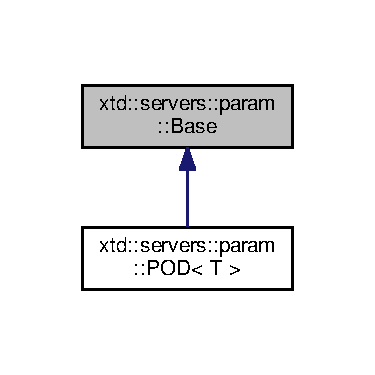
\includegraphics[width=181pt]{classxtd_1_1servers_1_1param_1_1Base__inherit__graph}
\end{center}
\end{figure}
\subsection*{Public Types}
\begin{DoxyCompactItemize}
\item 
typedef boost\+::shared\+\_\+ptr$<$ \hyperlink{classxtd_1_1servers_1_1param_1_1Base}{Base} $>$ \hyperlink{classxtd_1_1servers_1_1param_1_1Base_aaf4d92eca642f61cb81524096926c6a1}{t\+\_\+sptr}
\end{DoxyCompactItemize}
\subsection*{Public Member Functions}
\begin{DoxyCompactItemize}
\item 
{\footnotesize template$<$typename T $>$ }\\\hyperlink{classxtd_1_1servers_1_1param_1_1Base_ae7148147e419f2a3e5b27929e8b99b54}{Base} (const T \&p\+\_\+value)
\item 
{\footnotesize template$<$typename T $>$ }\\\hyperlink{classxtd_1_1servers_1_1param_1_1Base_aeadfa5af86a0dd70c6068a994f7ff567}{Base} (const T \&p\+\_\+value, const string \&p\+\_\+name)
\item 
virtual bool \hyperlink{classxtd_1_1servers_1_1param_1_1Base_a74a64bb56c20b892c9be9b786a2d94d1}{from\+Str} (const string \&p\+\_\+src)=0
\item 
virtual bool \hyperlink{classxtd_1_1servers_1_1param_1_1Base_a74d9a61d65e6e66492b2205489d9b2cf}{verify} (const string \&p\+\_\+src)=0
\item 
virtual bool \hyperlink{classxtd_1_1servers_1_1param_1_1Base_ab80c9c70cacf5a8cebb98486fba83116}{to\+Str} (string \&p\+\_\+dst) const =0
\item 
virtual void \hyperlink{classxtd_1_1servers_1_1param_1_1Base_a37a0c2247274dce2395517186ec70d7a}{accept} (\hyperlink{classxtd_1_1servers_1_1param_1_1Visitor}{Visitor} \&p\+\_\+visitor) const =0
\item 
string \hyperlink{classxtd_1_1servers_1_1param_1_1Base_a1e688aa518e874229d45a348c7596c82}{get\+Name} (void) const 
\begin{DoxyCompactList}\small\item\em Get parameter name. \end{DoxyCompactList}\item 
void \hyperlink{classxtd_1_1servers_1_1param_1_1Base_af0a668bb0360d7c2a8821527888d16d2}{set\+Name} (const string \&p\+\_\+name)
\begin{DoxyCompactList}\small\item\em Set parameter name. \end{DoxyCompactList}\item 
bool \hyperlink{classxtd_1_1servers_1_1param_1_1Base_a3d83345a6e83bbe96cb7e13c81061c7d}{get\+Sync} (void) const 
\begin{DoxyCompactList}\small\item\em Get sync property. \end{DoxyCompactList}\item 
void \hyperlink{classxtd_1_1servers_1_1param_1_1Base_a912fb989f6ecb224596add4d0b388102}{set\+Sync} (const bool \&p\+\_\+sync)
\begin{DoxyCompactList}\small\item\em Set sync property. \end{DoxyCompactList}\item 
void \hyperlink{classxtd_1_1servers_1_1param_1_1Base_a824470386f5a0f25824b6be50d15a38a}{set\+Action\+Path} (const string \&p\+\_\+action\+Path)
\begin{DoxyCompactList}\small\item\em Specify filesystem path to synchronize the parameter. \end{DoxyCompactList}\item 
string \hyperlink{classxtd_1_1servers_1_1param_1_1Base_a69c3c92644e04f22b9dba10095b0ed3b}{get\+Action\+Path} (void) const 
\begin{DoxyCompactList}\small\item\em Get the filesystem path. \end{DoxyCompactList}\item 
void \hyperlink{classxtd_1_1servers_1_1param_1_1Base_a74c2c5e1bac271ebbb80b93c1b976b47}{sync} (void)
\begin{DoxyCompactList}\small\item\em Process synchronization action. \end{DoxyCompactList}\item 
uint32\+\_\+t \hyperlink{classxtd_1_1servers_1_1param_1_1Base_a532c7d291a15c2d611af8ab9898239f2}{date} (void) const 
\begin{DoxyCompactList}\small\item\em Get last parameter change date. \end{DoxyCompactList}\item 
\hyperlink{classxtd_1_1servers_1_1param_1_1Base}{Base} \& \hyperlink{classxtd_1_1servers_1_1param_1_1Base_aeafea08d04f6c7af78014a4991f38b57}{constraint} (t\+\_\+constraint p\+\_\+constraint)
\begin{DoxyCompactList}\small\item\em Add a specific constraint the parameter must conform to. \end{DoxyCompactList}\item 
\hyperlink{classxtd_1_1servers_1_1param_1_1Base}{Base} \& \hyperlink{classxtd_1_1servers_1_1param_1_1Base_a819665d57d109485c4ba16352efc75e3}{listen} (t\+\_\+listener p\+\_\+listener)
\begin{DoxyCompactList}\small\item\em Specify the setter to modify the parameter. \end{DoxyCompactList}\item 
{\footnotesize template$<$typename T $>$ }\\\hyperlink{classxtd_1_1servers_1_1param_1_1Base}{Base} \& \hyperlink{classxtd_1_1servers_1_1param_1_1Base_afa9ec13039176f5e8da4c1ac6dfd4063}{constraint} (boost\+::function$<$ bool(const T \&)$>$ p\+\_\+constraint)
\begin{DoxyCompactList}\small\item\em Add a specific constraint the parameter must conform to. \end{DoxyCompactList}\item 
{\footnotesize template$<$typename T $>$ }\\\hyperlink{classxtd_1_1servers_1_1param_1_1Base}{Base} \& \hyperlink{classxtd_1_1servers_1_1param_1_1Base_af34d052ef13b435479838c0372f1edb2}{listen} (boost\+::function$<$ void(const T \&, const T \&)$>$ p\+\_\+constraint)
\begin{DoxyCompactList}\small\item\em Specify the setter to modify the parameter. \end{DoxyCompactList}\item 
{\footnotesize template$<$typename T $>$ }\\bool \hyperlink{classxtd_1_1servers_1_1param_1_1Base_a6161111b66cf64a5b953bd978b498fe8}{is\+Accepted} (const T \&p\+\_\+src)
\begin{DoxyCompactList}\small\item\em Tells if value is accepted by parameter. \end{DoxyCompactList}\item 
{\footnotesize template$<$typename T $>$ }\\bool \hyperlink{classxtd_1_1servers_1_1param_1_1Base_abff2c36296d9d309baafe94e7fd65834}{set} (const T \&p\+\_\+src)
\begin{DoxyCompactList}\small\item\em Function to set the parameter. \end{DoxyCompactList}\item 
void \hyperlink{classxtd_1_1servers_1_1param_1_1Base_a47d5b5e494732932d25fa992e0a06190}{set\+Log} (const string p\+\_\+log)
\begin{DoxyCompactList}\small\item\em Function to set log associated to parameter. \end{DoxyCompactList}\item 
{\footnotesize template$<$typename T $>$ }\\bool \hyperlink{classxtd_1_1servers_1_1param_1_1Base_a48c6b4f36d84c640cc68b347090a6ec5}{get} (T \&p\+\_\+dst) const 
\begin{DoxyCompactList}\small\item\em Function to get the parameter. \end{DoxyCompactList}\item 
string \hyperlink{classxtd_1_1servers_1_1param_1_1Base_a48e7dac1fe3c43d62057e7a92e4bece9}{log} () const 
\begin{DoxyCompactList}\small\item\em Function to get log associated to parameter. \end{DoxyCompactList}\end{DoxyCompactItemize}
\subsection*{Static Public Member Functions}
\begin{DoxyCompactItemize}
\item 
{\footnotesize template$<$typename T $>$ }\\static T \hyperlink{classxtd_1_1servers_1_1param_1_1Base_a6769f7c5e389cfd805e71634e774c329}{cast} (const boost\+::any \&p\+\_\+val)
\begin{DoxyCompactList}\small\item\em Generic cast. \end{DoxyCompactList}\end{DoxyCompactItemize}


\subsection{Detailed Description}
Param base class. 

provide generic methods to handle generic parameters 

Definition at line 27 of file Base.\+hh.



\subsection{Member Typedef Documentation}
\index{xtd\+::servers\+::param\+::\+Base@{xtd\+::servers\+::param\+::\+Base}!t\+\_\+sptr@{t\+\_\+sptr}}
\index{t\+\_\+sptr@{t\+\_\+sptr}!xtd\+::servers\+::param\+::\+Base@{xtd\+::servers\+::param\+::\+Base}}
\subsubsection[{\texorpdfstring{t\+\_\+sptr}{t_sptr}}]{\setlength{\rightskip}{0pt plus 5cm}typedef boost\+::shared\+\_\+ptr$<${\bf Base}$>$ {\bf xtd\+::servers\+::param\+::\+Base\+::t\+\_\+sptr}}\hypertarget{classxtd_1_1servers_1_1param_1_1Base_aaf4d92eca642f61cb81524096926c6a1}{}\label{classxtd_1_1servers_1_1param_1_1Base_aaf4d92eca642f61cb81524096926c6a1}


Definition at line 42 of file Base.\+hh.



\subsection{Constructor \& Destructor Documentation}
\index{xtd\+::servers\+::param\+::\+Base@{xtd\+::servers\+::param\+::\+Base}!Base@{Base}}
\index{Base@{Base}!xtd\+::servers\+::param\+::\+Base@{xtd\+::servers\+::param\+::\+Base}}
\subsubsection[{\texorpdfstring{Base(const T \&p\+\_\+value)}{Base(const T &p_value)}}]{\setlength{\rightskip}{0pt plus 5cm}template$<$typename T $>$ xtd\+::servers\+::param\+::\+Base\+::\+Base (
\begin{DoxyParamCaption}
\item[{const T \&}]{p\+\_\+value}
\end{DoxyParamCaption}
)}\hypertarget{classxtd_1_1servers_1_1param_1_1Base_ae7148147e419f2a3e5b27929e8b99b54}{}\label{classxtd_1_1servers_1_1param_1_1Base_ae7148147e419f2a3e5b27929e8b99b54}


Definition at line 291 of file Base.\+hh.


\begin{DoxyCode}
291                            :
292   m\_value(p\_value),
293   m\_defaultValue(p\_value),
294   m\_constraints(),
295   m\_listeners(),
296   m\_name(),
297   m\_sync(\textcolor{keyword}{true}),
298   m\_actionPath(\textcolor{stringliteral}{""}),
299   m\_timestamp(boost::posix\_time::microsec\_clock::local\_time()),
300   m\_log(\textcolor{stringliteral}{"no log"})
301 \{
302 \}
\end{DoxyCode}
\index{xtd\+::servers\+::param\+::\+Base@{xtd\+::servers\+::param\+::\+Base}!Base@{Base}}
\index{Base@{Base}!xtd\+::servers\+::param\+::\+Base@{xtd\+::servers\+::param\+::\+Base}}
\subsubsection[{\texorpdfstring{Base(const T \&p\+\_\+value, const string \&p\+\_\+name)}{Base(const T &p_value, const string &p_name)}}]{\setlength{\rightskip}{0pt plus 5cm}template$<$typename T $>$ xtd\+::servers\+::param\+::\+Base\+::\+Base (
\begin{DoxyParamCaption}
\item[{const T \&}]{p\+\_\+value, }
\item[{const string \&}]{p\+\_\+name}
\end{DoxyParamCaption}
)}\hypertarget{classxtd_1_1servers_1_1param_1_1Base_aeadfa5af86a0dd70c6068a994f7ff567}{}\label{classxtd_1_1servers_1_1param_1_1Base_aeadfa5af86a0dd70c6068a994f7ff567}


Definition at line 306 of file Base.\+hh.


\begin{DoxyCode}
306                                                  :
307   m\_value(p\_value),
308   m\_defaultValue(p\_value),
309   m\_constraints(),
310   m\_listeners(),
311   m\_name(p\_name),
312   m\_sync(\textcolor{keyword}{true}),
313   m\_actionPath(\textcolor{stringliteral}{""}),
314   m\_timestamp(boost::posix\_time::microsec\_clock::local\_time()),
315   m\_log(\textcolor{stringliteral}{"no log"})
316 \{
317 \}
\end{DoxyCode}


\subsection{Member Function Documentation}
\index{xtd\+::servers\+::param\+::\+Base@{xtd\+::servers\+::param\+::\+Base}!accept@{accept}}
\index{accept@{accept}!xtd\+::servers\+::param\+::\+Base@{xtd\+::servers\+::param\+::\+Base}}
\subsubsection[{\texorpdfstring{accept(\+Visitor \&p\+\_\+visitor) const =0}{accept(Visitor &p_visitor) const =0}}]{\setlength{\rightskip}{0pt plus 5cm}virtual void xtd\+::servers\+::param\+::\+Base\+::accept (
\begin{DoxyParamCaption}
\item[{{\bf Visitor} \&}]{p\+\_\+visitor}
\end{DoxyParamCaption}
) const\hspace{0.3cm}{\ttfamily [pure virtual]}}\hypertarget{classxtd_1_1servers_1_1param_1_1Base_a37a0c2247274dce2395517186ec70d7a}{}\label{classxtd_1_1servers_1_1param_1_1Base_a37a0c2247274dce2395517186ec70d7a}


Implemented in \hyperlink{classxtd_1_1servers_1_1param_1_1POD_a828a1fa2391bc087f396b87a1d7c793a}{xtd\+::servers\+::param\+::\+P\+O\+D$<$ T $>$}.

\index{xtd\+::servers\+::param\+::\+Base@{xtd\+::servers\+::param\+::\+Base}!cast@{cast}}
\index{cast@{cast}!xtd\+::servers\+::param\+::\+Base@{xtd\+::servers\+::param\+::\+Base}}
\subsubsection[{\texorpdfstring{cast(const boost\+::any \&p\+\_\+val)}{cast(const boost::any &p_val)}}]{\setlength{\rightskip}{0pt plus 5cm}template$<$typename T $>$ T xtd\+::servers\+::param\+::\+Base\+::cast (
\begin{DoxyParamCaption}
\item[{const boost\+::any \&}]{p\+\_\+val}
\end{DoxyParamCaption}
)\hspace{0.3cm}{\ttfamily [static]}}\hypertarget{classxtd_1_1servers_1_1param_1_1Base_a6769f7c5e389cfd805e71634e774c329}{}\label{classxtd_1_1servers_1_1param_1_1Base_a6769f7c5e389cfd805e71634e774c329}


Generic cast. 

N/A


\begin{DoxyParams}{Parameters}
{\em p\+\_\+val} & generic instance reference \\
\hline
\end{DoxyParams}

\begin{DoxyTemplParams}{Template Parameters}
{\em T} & generic type \\
\hline
\end{DoxyTemplParams}
\begin{DoxyReturn}{Returns}
specific type 
\end{DoxyReturn}


Definition at line 284 of file Base.\+hh.


\begin{DoxyCode}
285 \{
286   \textcolor{keywordflow}{return} boost::any\_cast<T>(p\_val);
287 \}
\end{DoxyCode}
\index{xtd\+::servers\+::param\+::\+Base@{xtd\+::servers\+::param\+::\+Base}!constraint@{constraint}}
\index{constraint@{constraint}!xtd\+::servers\+::param\+::\+Base@{xtd\+::servers\+::param\+::\+Base}}
\subsubsection[{\texorpdfstring{constraint(t\+\_\+constraint p\+\_\+constraint)}{constraint(t_constraint p_constraint)}}]{\setlength{\rightskip}{0pt plus 5cm}{\bf Base}\& xtd\+::servers\+::param\+::\+Base\+::constraint (
\begin{DoxyParamCaption}
\item[{t\+\_\+constraint}]{p\+\_\+constraint}
\end{DoxyParamCaption}
)}\hypertarget{classxtd_1_1servers_1_1param_1_1Base_aeafea08d04f6c7af78014a4991f38b57}{}\label{classxtd_1_1servers_1_1param_1_1Base_aeafea08d04f6c7af78014a4991f38b57}


Add a specific constraint the parameter must conform to. 

Each time a modification is requested, the constraint will be checked Many constraints can be added, they will be checked in declaration order Opposite constraints must be avoided


\begin{DoxyParams}{Parameters}
{\em p\+\_\+constraint} & the constraint \\
\hline
\end{DoxyParams}
\begin{DoxyReturn}{Returns}
a self reference 
\end{DoxyReturn}
\index{xtd\+::servers\+::param\+::\+Base@{xtd\+::servers\+::param\+::\+Base}!constraint@{constraint}}
\index{constraint@{constraint}!xtd\+::servers\+::param\+::\+Base@{xtd\+::servers\+::param\+::\+Base}}
\subsubsection[{\texorpdfstring{constraint(boost\+::function$<$ bool(const T \&)$>$ p\+\_\+constraint)}{constraint(boost::function< bool(const T &)> p_constraint)}}]{\setlength{\rightskip}{0pt plus 5cm}template$<$typename T $>$ {\bf Base} \& xtd\+::servers\+::param\+::\+Base\+::constraint (
\begin{DoxyParamCaption}
\item[{boost\+::function$<$ bool(const T \&)$>$}]{p\+\_\+constraint}
\end{DoxyParamCaption}
)}\hypertarget{classxtd_1_1servers_1_1param_1_1Base_afa9ec13039176f5e8da4c1ac6dfd4063}{}\label{classxtd_1_1servers_1_1param_1_1Base_afa9ec13039176f5e8da4c1ac6dfd4063}


Add a specific constraint the parameter must conform to. 

Each time a modification is requested, the constraint will be checked Many constraints can be added, they will be checked in declaration order Opposite constraints must be avoided


\begin{DoxyParams}{Parameters}
{\em p\+\_\+constraint} & the constraint \\
\hline
\end{DoxyParams}
\begin{DoxyReturn}{Returns}
a self reference 
\end{DoxyReturn}


Definition at line 322 of file Base.\+hh.


\begin{DoxyCode}
323 \{
324   m\_constraints.push\_back(boost::bind(p\_constraint, boost::bind(cast<T>, \_1)));
325   \textcolor{keywordflow}{return} *\textcolor{keyword}{this};
326 \}
\end{DoxyCode}
\index{xtd\+::servers\+::param\+::\+Base@{xtd\+::servers\+::param\+::\+Base}!date@{date}}
\index{date@{date}!xtd\+::servers\+::param\+::\+Base@{xtd\+::servers\+::param\+::\+Base}}
\subsubsection[{\texorpdfstring{date(void) const }{date(void) const }}]{\setlength{\rightskip}{0pt plus 5cm}uint32\+\_\+t xtd\+::servers\+::param\+::\+Base\+::date (
\begin{DoxyParamCaption}
\item[{void}]{}
\end{DoxyParamCaption}
) const}\hypertarget{classxtd_1_1servers_1_1param_1_1Base_a532c7d291a15c2d611af8ab9898239f2}{}\label{classxtd_1_1servers_1_1param_1_1Base_a532c7d291a15c2d611af8ab9898239f2}


Get last parameter change date. 

N/A

\begin{DoxyReturn}{Returns}
the last parameter change 
\end{DoxyReturn}
\index{xtd\+::servers\+::param\+::\+Base@{xtd\+::servers\+::param\+::\+Base}!from\+Str@{from\+Str}}
\index{from\+Str@{from\+Str}!xtd\+::servers\+::param\+::\+Base@{xtd\+::servers\+::param\+::\+Base}}
\subsubsection[{\texorpdfstring{from\+Str(const string \&p\+\_\+src)=0}{fromStr(const string &p_src)=0}}]{\setlength{\rightskip}{0pt plus 5cm}virtual bool xtd\+::servers\+::param\+::\+Base\+::from\+Str (
\begin{DoxyParamCaption}
\item[{const string \&}]{p\+\_\+src}
\end{DoxyParamCaption}
)\hspace{0.3cm}{\ttfamily [pure virtual]}}\hypertarget{classxtd_1_1servers_1_1param_1_1Base_a74a64bb56c20b892c9be9b786a2d94d1}{}\label{classxtd_1_1servers_1_1param_1_1Base_a74a64bb56c20b892c9be9b786a2d94d1}


Implemented in \hyperlink{classxtd_1_1servers_1_1param_1_1POD_ac6754089526df6eb0eef539be830c668}{xtd\+::servers\+::param\+::\+P\+O\+D$<$ T $>$}.

\index{xtd\+::servers\+::param\+::\+Base@{xtd\+::servers\+::param\+::\+Base}!get@{get}}
\index{get@{get}!xtd\+::servers\+::param\+::\+Base@{xtd\+::servers\+::param\+::\+Base}}
\subsubsection[{\texorpdfstring{get(\+T \&p\+\_\+dst) const }{get(T &p_dst) const }}]{\setlength{\rightskip}{0pt plus 5cm}template$<$typename T $>$ bool xtd\+::servers\+::param\+::\+Base\+::get (
\begin{DoxyParamCaption}
\item[{T \&}]{p\+\_\+dst}
\end{DoxyParamCaption}
) const}\hypertarget{classxtd_1_1servers_1_1param_1_1Base_a48c6b4f36d84c640cc68b347090a6ec5}{}\label{classxtd_1_1servers_1_1param_1_1Base_a48c6b4f36d84c640cc68b347090a6ec5}


Function to get the parameter. 

N/A


\begin{DoxyParams}{Parameters}
{\em p\+\_\+dst} & the current value \\
\hline
\end{DoxyParams}
\begin{DoxyReturn}{Returns}
true if getting succeeds 
\end{DoxyReturn}


Definition at line 332 of file Base.\+hh.


\begin{DoxyCode}
333 \{
334   \textcolor{keywordflow}{try} \{
335     p\_dst = boost::any\_cast<T>(m\_value);
336     \textcolor{keywordflow}{return} \textcolor{keyword}{true};
337   \}
338   \textcolor{keywordflow}{catch} (boost::bad\_any\_cast l\_error) \{
339     logger::crit(\textcolor{stringliteral}{"servers.param.base"}, \textcolor{stringliteral}{"unable to cast param '%s' as destination type (%s)"}, m\_name, 
      l\_error.what(), HERE);
340     \textcolor{keywordflow}{return} \textcolor{keyword}{false};
341   \}
342 \}
\end{DoxyCode}
\index{xtd\+::servers\+::param\+::\+Base@{xtd\+::servers\+::param\+::\+Base}!get\+Action\+Path@{get\+Action\+Path}}
\index{get\+Action\+Path@{get\+Action\+Path}!xtd\+::servers\+::param\+::\+Base@{xtd\+::servers\+::param\+::\+Base}}
\subsubsection[{\texorpdfstring{get\+Action\+Path(void) const }{getActionPath(void) const }}]{\setlength{\rightskip}{0pt plus 5cm}string xtd\+::servers\+::param\+::\+Base\+::get\+Action\+Path (
\begin{DoxyParamCaption}
\item[{void}]{}
\end{DoxyParamCaption}
) const}\hypertarget{classxtd_1_1servers_1_1param_1_1Base_a69c3c92644e04f22b9dba10095b0ed3b}{}\label{classxtd_1_1servers_1_1param_1_1Base_a69c3c92644e04f22b9dba10095b0ed3b}


Get the filesystem path. 

N/A \begin{DoxyReturn}{Returns}
the filesystem path 
\end{DoxyReturn}
\index{xtd\+::servers\+::param\+::\+Base@{xtd\+::servers\+::param\+::\+Base}!get\+Name@{get\+Name}}
\index{get\+Name@{get\+Name}!xtd\+::servers\+::param\+::\+Base@{xtd\+::servers\+::param\+::\+Base}}
\subsubsection[{\texorpdfstring{get\+Name(void) const }{getName(void) const }}]{\setlength{\rightskip}{0pt plus 5cm}string xtd\+::servers\+::param\+::\+Base\+::get\+Name (
\begin{DoxyParamCaption}
\item[{void}]{}
\end{DoxyParamCaption}
) const}\hypertarget{classxtd_1_1servers_1_1param_1_1Base_a1e688aa518e874229d45a348c7596c82}{}\label{classxtd_1_1servers_1_1param_1_1Base_a1e688aa518e874229d45a348c7596c82}


Get parameter name. 

N/A \begin{DoxyReturn}{Returns}
associated name 
\end{DoxyReturn}
\index{xtd\+::servers\+::param\+::\+Base@{xtd\+::servers\+::param\+::\+Base}!get\+Sync@{get\+Sync}}
\index{get\+Sync@{get\+Sync}!xtd\+::servers\+::param\+::\+Base@{xtd\+::servers\+::param\+::\+Base}}
\subsubsection[{\texorpdfstring{get\+Sync(void) const }{getSync(void) const }}]{\setlength{\rightskip}{0pt plus 5cm}bool xtd\+::servers\+::param\+::\+Base\+::get\+Sync (
\begin{DoxyParamCaption}
\item[{void}]{}
\end{DoxyParamCaption}
) const}\hypertarget{classxtd_1_1servers_1_1param_1_1Base_a3d83345a6e83bbe96cb7e13c81061c7d}{}\label{classxtd_1_1servers_1_1param_1_1Base_a3d83345a6e83bbe96cb7e13c81061c7d}


Get sync property. 

\mbox{[}long description\mbox{]} \begin{DoxyReturn}{Returns}
true if the parameter needs to be synchronized on the filesystem else false 
\end{DoxyReturn}
\index{xtd\+::servers\+::param\+::\+Base@{xtd\+::servers\+::param\+::\+Base}!is\+Accepted@{is\+Accepted}}
\index{is\+Accepted@{is\+Accepted}!xtd\+::servers\+::param\+::\+Base@{xtd\+::servers\+::param\+::\+Base}}
\subsubsection[{\texorpdfstring{is\+Accepted(const T \&p\+\_\+src)}{isAccepted(const T &p_src)}}]{\setlength{\rightskip}{0pt plus 5cm}template$<$typename T $>$ bool xtd\+::servers\+::param\+::\+Base\+::is\+Accepted (
\begin{DoxyParamCaption}
\item[{const T \&}]{p\+\_\+src}
\end{DoxyParamCaption}
)}\hypertarget{classxtd_1_1servers_1_1param_1_1Base_a6161111b66cf64a5b953bd978b498fe8}{}\label{classxtd_1_1servers_1_1param_1_1Base_a6161111b66cf64a5b953bd978b498fe8}


Tells if value is accepted by parameter. 

N/A


\begin{DoxyParams}{Parameters}
{\em p\+\_\+src} & the new value \\
\hline
\end{DoxyParams}
\begin{DoxyReturn}{Returns}
true if value is accepted 
\end{DoxyReturn}


Definition at line 347 of file Base.\+hh.


\begin{DoxyCode}
348 \{
349   \textcolor{comment}{// Verify type}
350   \textcolor{keywordflow}{if} (\textcolor{keyword}{typeid}(T) != m\_defaultValue.type())
351     \textcolor{keywordflow}{return} \textcolor{keyword}{false};
352 
353   \textcolor{comment}{// Verify constraints}
354   BOOST\_FOREACH(\textcolor{keyword}{const} t\_constraint& c\_cond, m\_constraints)
355   \{
356     \textcolor{keywordflow}{if} (\textcolor{keyword}{false} == c\_cond(p\_src))
357       \textcolor{keywordflow}{return} \textcolor{keyword}{false};
358   \}
359 
360   \textcolor{keywordflow}{return} \textcolor{keyword}{true};
361 \}
\end{DoxyCode}


Here is the caller graph for this function\+:
\nopagebreak
\begin{figure}[H]
\begin{center}
\leavevmode
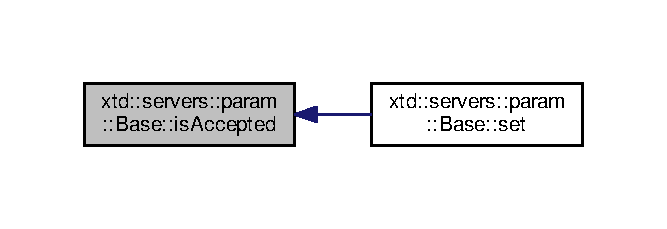
\includegraphics[width=318pt]{classxtd_1_1servers_1_1param_1_1Base_a6161111b66cf64a5b953bd978b498fe8_icgraph}
\end{center}
\end{figure}


\index{xtd\+::servers\+::param\+::\+Base@{xtd\+::servers\+::param\+::\+Base}!listen@{listen}}
\index{listen@{listen}!xtd\+::servers\+::param\+::\+Base@{xtd\+::servers\+::param\+::\+Base}}
\subsubsection[{\texorpdfstring{listen(t\+\_\+listener p\+\_\+listener)}{listen(t_listener p_listener)}}]{\setlength{\rightskip}{0pt plus 5cm}{\bf Base}\& xtd\+::servers\+::param\+::\+Base\+::listen (
\begin{DoxyParamCaption}
\item[{t\+\_\+listener}]{p\+\_\+listener}
\end{DoxyParamCaption}
)}\hypertarget{classxtd_1_1servers_1_1param_1_1Base_a819665d57d109485c4ba16352efc75e3}{}\label{classxtd_1_1servers_1_1param_1_1Base_a819665d57d109485c4ba16352efc75e3}


Specify the setter to modify the parameter. 

This function will be called each time a call to set is done


\begin{DoxyParams}{Parameters}
{\em p\+\_\+listener} & a modification function \\
\hline
\end{DoxyParams}
\begin{DoxyReturn}{Returns}
a self reference 
\end{DoxyReturn}
\index{xtd\+::servers\+::param\+::\+Base@{xtd\+::servers\+::param\+::\+Base}!listen@{listen}}
\index{listen@{listen}!xtd\+::servers\+::param\+::\+Base@{xtd\+::servers\+::param\+::\+Base}}
\subsubsection[{\texorpdfstring{listen(boost\+::function$<$ void(const T \&, const T \&)$>$ p\+\_\+constraint)}{listen(boost::function< void(const T &, const T &)> p_constraint)}}]{\setlength{\rightskip}{0pt plus 5cm}template$<$typename T $>$ {\bf Base} \& xtd\+::servers\+::param\+::\+Base\+::listen (
\begin{DoxyParamCaption}
\item[{boost\+::function$<$ void(const T \&, const T \&)$>$}]{p\+\_\+constraint}
\end{DoxyParamCaption}
)}\hypertarget{classxtd_1_1servers_1_1param_1_1Base_af34d052ef13b435479838c0372f1edb2}{}\label{classxtd_1_1servers_1_1param_1_1Base_af34d052ef13b435479838c0372f1edb2}


Specify the setter to modify the parameter. 

This function will be called each time a call to set is done 
\begin{DoxyParams}{Parameters}
{\em p\+\_\+constraint} & a modification function \\
\hline
\end{DoxyParams}
\begin{DoxyReturn}{Returns}
a self reference 
\end{DoxyReturn}


Definition at line 396 of file Base.\+hh.


\begin{DoxyCode}
397 \{
398   m\_listeners.push\_back(boost::bind(p\_constraint,
399                                     boost::bind(cast<T>, \_1),
400                                     boost::bind(cast<T>, \_2)));
401   \textcolor{keywordflow}{return} *\textcolor{keyword}{this};
402 \}
\end{DoxyCode}
\index{xtd\+::servers\+::param\+::\+Base@{xtd\+::servers\+::param\+::\+Base}!log@{log}}
\index{log@{log}!xtd\+::servers\+::param\+::\+Base@{xtd\+::servers\+::param\+::\+Base}}
\subsubsection[{\texorpdfstring{log() const }{log() const }}]{\setlength{\rightskip}{0pt plus 5cm}string xtd\+::servers\+::param\+::\+Base\+::log (
\begin{DoxyParamCaption}
{}
\end{DoxyParamCaption}
) const}\hypertarget{classxtd_1_1servers_1_1param_1_1Base_a48e7dac1fe3c43d62057e7a92e4bece9}{}\label{classxtd_1_1servers_1_1param_1_1Base_a48e7dac1fe3c43d62057e7a92e4bece9}


Function to get log associated to parameter. 

N/A

\begin{DoxyReturn}{Returns}
log associated with parameter 
\end{DoxyReturn}
\index{xtd\+::servers\+::param\+::\+Base@{xtd\+::servers\+::param\+::\+Base}!set@{set}}
\index{set@{set}!xtd\+::servers\+::param\+::\+Base@{xtd\+::servers\+::param\+::\+Base}}
\subsubsection[{\texorpdfstring{set(const T \&p\+\_\+src)}{set(const T &p_src)}}]{\setlength{\rightskip}{0pt plus 5cm}template$<$typename T $>$ bool xtd\+::servers\+::param\+::\+Base\+::set (
\begin{DoxyParamCaption}
\item[{const T \&}]{p\+\_\+src}
\end{DoxyParamCaption}
)}\hypertarget{classxtd_1_1servers_1_1param_1_1Base_abff2c36296d9d309baafe94e7fd65834}{}\label{classxtd_1_1servers_1_1param_1_1Base_abff2c36296d9d309baafe94e7fd65834}


Function to set the parameter. 

N/A


\begin{DoxyParams}{Parameters}
{\em p\+\_\+src} & the new value \\
\hline
\end{DoxyParams}
\begin{DoxyReturn}{Returns}
true if setting succeeds 
\end{DoxyReturn}


Definition at line 365 of file Base.\+hh.


\begin{DoxyCode}
366 \{
367   T l\_value;
368 
369   \textcolor{keywordflow}{if} (\textcolor{keyword}{false} == \hyperlink{classxtd_1_1servers_1_1param_1_1Base_a6161111b66cf64a5b953bd978b498fe8}{isAccepted}(p\_src))
370     \textcolor{keywordflow}{return} \textcolor{keyword}{false};
371 
372   \textcolor{comment}{// Update timestamp last parameter access}
373   m\_timestamp = boost::posix\_time::microsec\_clock::local\_time();
374 
375   \textcolor{comment}{// If new value is different, update value and trace parameter change}
376   \textcolor{keywordflow}{if} (\textcolor{keyword}{true} == \textcolor{keyword}{get}(l\_value) && (l\_value != p\_src))
377   \{
378     \textcolor{keywordtype}{string} l\_oldStr, l\_newStr;
379     boost::any  l\_old = m\_value;
380 
381     \hyperlink{classxtd_1_1servers_1_1param_1_1Base_ab80c9c70cacf5a8cebb98486fba83116}{toStr}(l\_oldStr);
382     m\_value = p\_src;
383     \hyperlink{classxtd_1_1servers_1_1param_1_1Base_ab80c9c70cacf5a8cebb98486fba83116}{toStr}(l\_newStr);
384 
385     logger::crit(\textcolor{stringliteral}{"servers.param.base"}, \textcolor{stringliteral}{"parameter '%s' has been changed from '%s' to '%s'"}, m\_name, 
      l\_oldStr, l\_newStr, HERE);
386 
387     \textcolor{keywordflow}{for} (\textcolor{keyword}{auto}& c\_callback : m\_listeners)
388       c\_callback(l\_old, m\_value);
389   \}
390 
391   \textcolor{keywordflow}{return} \textcolor{keyword}{true};
392 \}
\end{DoxyCode}


Here is the call graph for this function\+:
\nopagebreak
\begin{figure}[H]
\begin{center}
\leavevmode
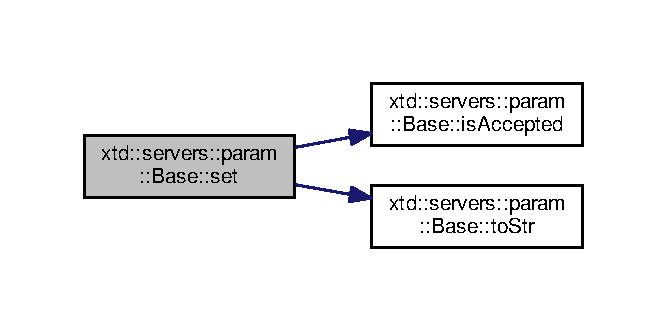
\includegraphics[width=318pt]{classxtd_1_1servers_1_1param_1_1Base_abff2c36296d9d309baafe94e7fd65834_cgraph}
\end{center}
\end{figure}


\index{xtd\+::servers\+::param\+::\+Base@{xtd\+::servers\+::param\+::\+Base}!set\+Action\+Path@{set\+Action\+Path}}
\index{set\+Action\+Path@{set\+Action\+Path}!xtd\+::servers\+::param\+::\+Base@{xtd\+::servers\+::param\+::\+Base}}
\subsubsection[{\texorpdfstring{set\+Action\+Path(const string \&p\+\_\+action\+Path)}{setActionPath(const string &p_actionPath)}}]{\setlength{\rightskip}{0pt plus 5cm}void xtd\+::servers\+::param\+::\+Base\+::set\+Action\+Path (
\begin{DoxyParamCaption}
\item[{const string \&}]{p\+\_\+action\+Path}
\end{DoxyParamCaption}
)}\hypertarget{classxtd_1_1servers_1_1param_1_1Base_a824470386f5a0f25824b6be50d15a38a}{}\label{classxtd_1_1servers_1_1param_1_1Base_a824470386f5a0f25824b6be50d15a38a}


Specify filesystem path to synchronize the parameter. 

N/A


\begin{DoxyParams}{Parameters}
{\em p\+\_\+action\+Path} & filesystem path \\
\hline
\end{DoxyParams}
\index{xtd\+::servers\+::param\+::\+Base@{xtd\+::servers\+::param\+::\+Base}!set\+Log@{set\+Log}}
\index{set\+Log@{set\+Log}!xtd\+::servers\+::param\+::\+Base@{xtd\+::servers\+::param\+::\+Base}}
\subsubsection[{\texorpdfstring{set\+Log(const string p\+\_\+log)}{setLog(const string p_log)}}]{\setlength{\rightskip}{0pt plus 5cm}void xtd\+::servers\+::param\+::\+Base\+::set\+Log (
\begin{DoxyParamCaption}
\item[{const string}]{p\+\_\+log}
\end{DoxyParamCaption}
)}\hypertarget{classxtd_1_1servers_1_1param_1_1Base_a47d5b5e494732932d25fa992e0a06190}{}\label{classxtd_1_1servers_1_1param_1_1Base_a47d5b5e494732932d25fa992e0a06190}


Function to set log associated to parameter. 

N/A


\begin{DoxyParams}{Parameters}
{\em p\+\_\+log} & \\
\hline
\end{DoxyParams}
\index{xtd\+::servers\+::param\+::\+Base@{xtd\+::servers\+::param\+::\+Base}!set\+Name@{set\+Name}}
\index{set\+Name@{set\+Name}!xtd\+::servers\+::param\+::\+Base@{xtd\+::servers\+::param\+::\+Base}}
\subsubsection[{\texorpdfstring{set\+Name(const string \&p\+\_\+name)}{setName(const string &p_name)}}]{\setlength{\rightskip}{0pt plus 5cm}void xtd\+::servers\+::param\+::\+Base\+::set\+Name (
\begin{DoxyParamCaption}
\item[{const string \&}]{p\+\_\+name}
\end{DoxyParamCaption}
)}\hypertarget{classxtd_1_1servers_1_1param_1_1Base_af0a668bb0360d7c2a8821527888d16d2}{}\label{classxtd_1_1servers_1_1param_1_1Base_af0a668bb0360d7c2a8821527888d16d2}


Set parameter name. 

N/A


\begin{DoxyParams}{Parameters}
{\em p\+\_\+name} & requested name \\
\hline
\end{DoxyParams}
\index{xtd\+::servers\+::param\+::\+Base@{xtd\+::servers\+::param\+::\+Base}!set\+Sync@{set\+Sync}}
\index{set\+Sync@{set\+Sync}!xtd\+::servers\+::param\+::\+Base@{xtd\+::servers\+::param\+::\+Base}}
\subsubsection[{\texorpdfstring{set\+Sync(const bool \&p\+\_\+sync)}{setSync(const bool &p_sync)}}]{\setlength{\rightskip}{0pt plus 5cm}void xtd\+::servers\+::param\+::\+Base\+::set\+Sync (
\begin{DoxyParamCaption}
\item[{const bool \&}]{p\+\_\+sync}
\end{DoxyParamCaption}
)}\hypertarget{classxtd_1_1servers_1_1param_1_1Base_a912fb989f6ecb224596add4d0b388102}{}\label{classxtd_1_1servers_1_1param_1_1Base_a912fb989f6ecb224596add4d0b388102}


Set sync property. 

N/A


\begin{DoxyParams}{Parameters}
{\em p\+\_\+sync} & requested sync property \\
\hline
\end{DoxyParams}
\index{xtd\+::servers\+::param\+::\+Base@{xtd\+::servers\+::param\+::\+Base}!sync@{sync}}
\index{sync@{sync}!xtd\+::servers\+::param\+::\+Base@{xtd\+::servers\+::param\+::\+Base}}
\subsubsection[{\texorpdfstring{sync(void)}{sync(void)}}]{\setlength{\rightskip}{0pt plus 5cm}void xtd\+::servers\+::param\+::\+Base\+::sync (
\begin{DoxyParamCaption}
\item[{void}]{}
\end{DoxyParamCaption}
)}\hypertarget{classxtd_1_1servers_1_1param_1_1Base_a74c2c5e1bac271ebbb80b93c1b976b47}{}\label{classxtd_1_1servers_1_1param_1_1Base_a74c2c5e1bac271ebbb80b93c1b976b47}


Process synchronization action. 

N/A \index{xtd\+::servers\+::param\+::\+Base@{xtd\+::servers\+::param\+::\+Base}!to\+Str@{to\+Str}}
\index{to\+Str@{to\+Str}!xtd\+::servers\+::param\+::\+Base@{xtd\+::servers\+::param\+::\+Base}}
\subsubsection[{\texorpdfstring{to\+Str(string \&p\+\_\+dst) const =0}{toStr(string &p_dst) const =0}}]{\setlength{\rightskip}{0pt plus 5cm}virtual bool xtd\+::servers\+::param\+::\+Base\+::to\+Str (
\begin{DoxyParamCaption}
\item[{string \&}]{p\+\_\+dst}
\end{DoxyParamCaption}
) const\hspace{0.3cm}{\ttfamily [pure virtual]}}\hypertarget{classxtd_1_1servers_1_1param_1_1Base_ab80c9c70cacf5a8cebb98486fba83116}{}\label{classxtd_1_1servers_1_1param_1_1Base_ab80c9c70cacf5a8cebb98486fba83116}


Implemented in \hyperlink{classxtd_1_1servers_1_1param_1_1POD_a6b40b7e5cd208c4ab848edb753c612f7}{xtd\+::servers\+::param\+::\+P\+O\+D$<$ T $>$}.



Here is the caller graph for this function\+:
\nopagebreak
\begin{figure}[H]
\begin{center}
\leavevmode
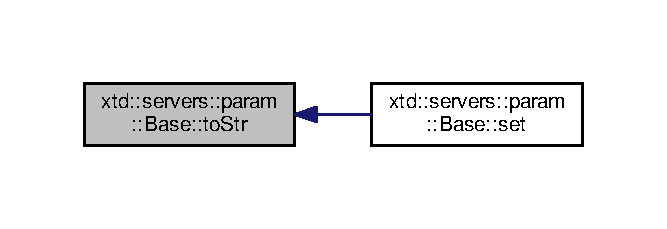
\includegraphics[width=318pt]{classxtd_1_1servers_1_1param_1_1Base_ab80c9c70cacf5a8cebb98486fba83116_icgraph}
\end{center}
\end{figure}


\index{xtd\+::servers\+::param\+::\+Base@{xtd\+::servers\+::param\+::\+Base}!verify@{verify}}
\index{verify@{verify}!xtd\+::servers\+::param\+::\+Base@{xtd\+::servers\+::param\+::\+Base}}
\subsubsection[{\texorpdfstring{verify(const string \&p\+\_\+src)=0}{verify(const string &p_src)=0}}]{\setlength{\rightskip}{0pt plus 5cm}virtual bool xtd\+::servers\+::param\+::\+Base\+::verify (
\begin{DoxyParamCaption}
\item[{const string \&}]{p\+\_\+src}
\end{DoxyParamCaption}
)\hspace{0.3cm}{\ttfamily [pure virtual]}}\hypertarget{classxtd_1_1servers_1_1param_1_1Base_a74d9a61d65e6e66492b2205489d9b2cf}{}\label{classxtd_1_1servers_1_1param_1_1Base_a74d9a61d65e6e66492b2205489d9b2cf}


Implemented in \hyperlink{classxtd_1_1servers_1_1param_1_1POD_aded664a97a02450a9270dd04af042d0c}{xtd\+::servers\+::param\+::\+P\+O\+D$<$ T $>$}.



The documentation for this class was generated from the following file\+:\begin{DoxyCompactItemize}
\item 
/home/psyco/dev/xtdcpp/servers/src/param/\hyperlink{Base_8hh}{Base.\+hh}\end{DoxyCompactItemize}

\hypertarget{classxtd_1_1servers_1_1param_1_1Handler}{}\section{xtd\+:\+:servers\+:\+:param\+:\+:Handler Class Reference}
\label{classxtd_1_1servers_1_1param_1_1Handler}\index{xtd\+::servers\+::param\+::\+Handler@{xtd\+::servers\+::param\+::\+Handler}}


Param handler class.  




{\ttfamily \#include $<$Handler.\+hh$>$}

\subsection*{Public Member Functions}
\begin{DoxyCompactItemize}
\item 
\hyperlink{classxtd_1_1servers_1_1param_1_1Handler_a93996915b562641b4673381c9abfae7b}{Handler} (const string \&p\+\_\+action\+Path)
\begin{DoxyCompactList}\small\item\em Constructor. \end{DoxyCompactList}\item 
{\footnotesize template$<$typename T $>$ }\\t\+\_\+param\+\_\+sptr \hyperlink{classxtd_1_1servers_1_1param_1_1Handler_a53a10d8d422013e62363e0d28d4e9017}{add} (const string \&p\+\_\+name, const T \&p\+\_\+val, bool p\+\_\+sync\+Disk=true)
\begin{DoxyCompactList}\small\item\em Add a new parameter to the \hyperlink{classxtd_1_1servers_1_1param_1_1Handler}{Handler}. \end{DoxyCompactList}\item 
{\footnotesize template$<$typename T $>$ }\\t\+\_\+param\+\_\+sptr \hyperlink{classxtd_1_1servers_1_1param_1_1Handler_a3bc858ae5bb7b6ce1f4d0a5eb327d17f}{bind} (const string \&p\+\_\+name, T \&p\+\_\+val, bool p\+\_\+sync\+Disk=true)
\item 
t\+\_\+param\+\_\+sptr \hyperlink{classxtd_1_1servers_1_1param_1_1Handler_a72a575bef0683ae6197c9f34cdf31d8f}{add} (const string \&p\+\_\+name, t\+\_\+param\+\_\+sptr p\+\_\+param, bool p\+\_\+sync\+Disk=true)
\begin{DoxyCompactList}\small\item\em Add a new parameter to the \hyperlink{classxtd_1_1servers_1_1param_1_1Handler}{Handler}. \end{DoxyCompactList}\item 
bool \hyperlink{classxtd_1_1servers_1_1param_1_1Handler_a0fcbef276a961d96584354588fc3bfcf}{exists} (const string \&p\+\_\+name)
\begin{DoxyCompactList}\small\item\em Existency checking. \end{DoxyCompactList}\item 
void \hyperlink{classxtd_1_1servers_1_1param_1_1Handler_a9533d788448e6bfdaf1c0f439a9f7b05}{initialize} (void)
\begin{DoxyCompactList}\small\item\em Initialization. \end{DoxyCompactList}\item 
void \hyperlink{classxtd_1_1servers_1_1param_1_1Handler_aba6e8d983f28617b3168b60cf6464926}{accept} (\hyperlink{classxtd_1_1servers_1_1param_1_1Visitor}{Visitor} \&p\+\_\+visitor) const 
\begin{DoxyCompactList}\small\item\em Add parameters to the Json visitor. \end{DoxyCompactList}\item 
bool \hyperlink{classxtd_1_1servers_1_1param_1_1Handler_aa2b60f898a67bd55c4289686591a2f3b}{verify} (const string \&p\+\_\+name, const string \&p\+\_\+src)
\begin{DoxyCompactList}\small\item\em Function to verify if given string value can be setted on parameter. \end{DoxyCompactList}\item 
bool \hyperlink{classxtd_1_1servers_1_1param_1_1Handler_ab3a53b8db70cf25c3e1de6425d876c37}{from\+Str} (const string \&p\+\_\+name, const string \&p\+\_\+src, const string \&p\+\_\+log)
\begin{DoxyCompactList}\small\item\em Retreive parameter value from a string. \end{DoxyCompactList}\item 
t\+\_\+params\+::iterator \hyperlink{classxtd_1_1servers_1_1param_1_1Handler_a66465c7a1ee0978f7558d55bfd8bd583}{find} (const string \&p\+\_\+name)
\begin{DoxyCompactList}\small\item\em return an iterator on a find call on map \end{DoxyCompactList}\item 
{\footnotesize template$<$typename T $>$ }\\bool \hyperlink{classxtd_1_1servers_1_1param_1_1Handler_a0f767078fd33fec21e1677d0a0195d8e}{get} (const string \&p\+\_\+name, T \&p\+\_\+dst)
\begin{DoxyCompactList}\small\item\em Get the current value of a parameter. \end{DoxyCompactList}\item 
{\footnotesize template$<$typename T $>$ }\\bool \hyperlink{classxtd_1_1servers_1_1param_1_1Handler_af8dbec0f2d639d39fb11605609462dee}{set} (const string \&p\+\_\+name, const T \&p\+\_\+src)
\begin{DoxyCompactList}\small\item\em Set a parameter value. \end{DoxyCompactList}\item 
{\footnotesize template$<$typename T $>$ }\\bool \hyperlink{classxtd_1_1servers_1_1param_1_1Handler_a3e71b80a00c962a862c1d3cc4d623c05}{listen} (const string \&p\+\_\+name, T p\+\_\+handler)
\begin{DoxyCompactList}\small\item\em Specify the setter to modify the parameter. \end{DoxyCompactList}\item 
{\footnotesize template$<$typename T $>$ }\\bool \hyperlink{classxtd_1_1servers_1_1param_1_1Handler_a20d689629d4748c14e4a516580a7c55a}{constraint} (const string \&p\+\_\+name, T p\+\_\+handler)
\begin{DoxyCompactList}\small\item\em Add a specific constraint to match while trying to modify a parameter. \end{DoxyCompactList}\end{DoxyCompactItemize}


\subsection{Detailed Description}
Param handler class. 

Store declared parameter in an internal map throw add method Provide get and set methods to modify already declared parameters 

Definition at line 25 of file Handler.\+hh.



\subsection{Constructor \& Destructor Documentation}
\index{xtd\+::servers\+::param\+::\+Handler@{xtd\+::servers\+::param\+::\+Handler}!Handler@{Handler}}
\index{Handler@{Handler}!xtd\+::servers\+::param\+::\+Handler@{xtd\+::servers\+::param\+::\+Handler}}
\subsubsection[{\texorpdfstring{Handler(const string \&p\+\_\+action\+Path)}{Handler(const string &p_actionPath)}}]{\setlength{\rightskip}{0pt plus 5cm}xtd\+::servers\+::param\+::\+Handler\+::\+Handler (
\begin{DoxyParamCaption}
\item[{const string \&}]{p\+\_\+action\+Path}
\end{DoxyParamCaption}
)}\hypertarget{classxtd_1_1servers_1_1param_1_1Handler_a93996915b562641b4673381c9abfae7b}{}\label{classxtd_1_1servers_1_1param_1_1Handler_a93996915b562641b4673381c9abfae7b}


Constructor. 

N/A


\begin{DoxyParams}{Parameters}
{\em p\+\_\+action\+Path} & the action path where to store persistent parameters (i.\+e. files containing values) \\
\hline
\end{DoxyParams}


Definition at line 26 of file Handler.\+cc.


\begin{DoxyCode}
26                                            :
27   m\_actionPath(p\_actionPath),
28   m\_params()
29 \{
30   \textcolor{keywordflow}{if} (\textcolor{keyword}{false} == is\_directory(m\_actionPath))
31   \{
32     logger::info(\textcolor{stringliteral}{"servers.param.handler"}, \textcolor{stringliteral}{"action directory '%s' does not exist, trying to create it"}, 
      m\_actionPath, HERE);
33     \textcolor{keywordflow}{if} (\textcolor{keyword}{false} == create\_directories(m\_actionPath))
34     \{
35       \textcolor{keywordflow}{if} (\textcolor{keyword}{false} == is\_directory(m\_actionPath))
36         error::do\_throw(\textcolor{stringliteral}{"servers.param.handler"}, \textcolor{stringliteral}{"failed to create action directory '%s', exit now!"}, 
      m\_actionPath, HERE);
37     \}
38     \textcolor{keywordflow}{else}
39     \{
40       logger::info(\textcolor{stringliteral}{"servers.param.handler"}, \textcolor{stringliteral}{"action directory '%s' created"}, m\_actionPath, HERE);
41     \}
42   \}
43 \}
\end{DoxyCode}


\subsection{Member Function Documentation}
\index{xtd\+::servers\+::param\+::\+Handler@{xtd\+::servers\+::param\+::\+Handler}!accept@{accept}}
\index{accept@{accept}!xtd\+::servers\+::param\+::\+Handler@{xtd\+::servers\+::param\+::\+Handler}}
\subsubsection[{\texorpdfstring{accept(\+Visitor \&p\+\_\+visitor) const }{accept(Visitor &p_visitor) const }}]{\setlength{\rightskip}{0pt plus 5cm}void xtd\+::servers\+::param\+::\+Handler\+::accept (
\begin{DoxyParamCaption}
\item[{{\bf Visitor} \&}]{p\+\_\+visitor}
\end{DoxyParamCaption}
) const}\hypertarget{classxtd_1_1servers_1_1param_1_1Handler_aba6e8d983f28617b3168b60cf6464926}{}\label{classxtd_1_1servers_1_1param_1_1Handler_aba6e8d983f28617b3168b60cf6464926}


Add parameters to the Json visitor. 

call accept on each parameter


\begin{DoxyParams}{Parameters}
{\em p\+\_\+visitor} & the right visitor \\
\hline
\end{DoxyParams}


Definition at line 119 of file Handler.\+cc.


\begin{DoxyCode}
120 \{
121   BOOST\_FOREACH(\textcolor{keyword}{const} t\_params::value\_type& c\_param, m\_params)
122     c\_param.second->\hyperlink{classxtd_1_1servers_1_1param_1_1Handler_aba6e8d983f28617b3168b60cf6464926}{accept}(p\_visitor);
123 \}
\end{DoxyCode}
\index{xtd\+::servers\+::param\+::\+Handler@{xtd\+::servers\+::param\+::\+Handler}!add@{add}}
\index{add@{add}!xtd\+::servers\+::param\+::\+Handler@{xtd\+::servers\+::param\+::\+Handler}}
\subsubsection[{\texorpdfstring{add(const string \&p\+\_\+name, const T \&p\+\_\+val, bool p\+\_\+sync\+Disk=true)}{add(const string &p_name, const T &p_val, bool p_syncDisk=true)}}]{\setlength{\rightskip}{0pt plus 5cm}template$<$typename T $>$ Handler\+::t\+\_\+param\+\_\+sptr xtd\+::servers\+::param\+::\+Handler\+::add (
\begin{DoxyParamCaption}
\item[{const string \&}]{p\+\_\+name, }
\item[{const T \&}]{p\+\_\+val, }
\item[{bool}]{p\+\_\+sync\+Disk = {\ttfamily true}}
\end{DoxyParamCaption}
)}\hypertarget{classxtd_1_1servers_1_1param_1_1Handler_a53a10d8d422013e62363e0d28d4e9017}{}\label{classxtd_1_1servers_1_1param_1_1Handler_a53a10d8d422013e62363e0d28d4e9017}


Add a new parameter to the \hyperlink{classxtd_1_1servers_1_1param_1_1Handler}{Handler}. 

N/A


\begin{DoxyParams}{Parameters}
{\em p\+\_\+name} & the key name for the parameter \\
\hline
{\em p\+\_\+val} & the the variable to register \\
\hline
{\em p\+\_\+sync\+Disk} & the persistence parameter \\
\hline
\end{DoxyParams}
\begin{DoxyReturn}{Returns}
a shared ptr to the base param object 
\end{DoxyReturn}


Definition at line 184 of file Handler.\+hh.


\begin{DoxyCode}
185 \{
186   t\_param\_sptr l\_param(\textcolor{keyword}{new} POD<T>(p\_val, p\_name));
187   \textcolor{keywordflow}{return} \hyperlink{classxtd_1_1servers_1_1param_1_1Handler_a53a10d8d422013e62363e0d28d4e9017}{add}(p\_name, l\_param, p\_syncDisk);
188 \}
\end{DoxyCode}


Here is the caller graph for this function\+:
\nopagebreak
\begin{figure}[H]
\begin{center}
\leavevmode
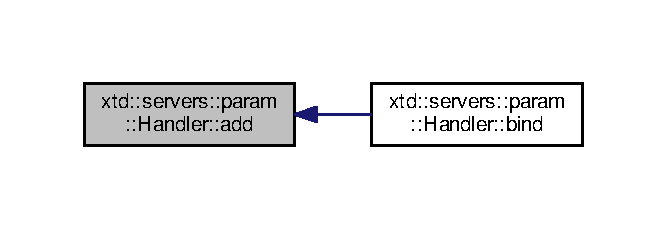
\includegraphics[width=318pt]{classxtd_1_1servers_1_1param_1_1Handler_a53a10d8d422013e62363e0d28d4e9017_icgraph}
\end{center}
\end{figure}


\index{xtd\+::servers\+::param\+::\+Handler@{xtd\+::servers\+::param\+::\+Handler}!add@{add}}
\index{add@{add}!xtd\+::servers\+::param\+::\+Handler@{xtd\+::servers\+::param\+::\+Handler}}
\subsubsection[{\texorpdfstring{add(const string \&p\+\_\+name, t\+\_\+param\+\_\+sptr p\+\_\+param, bool p\+\_\+sync\+Disk=true)}{add(const string &p_name, t_param_sptr p_param, bool p_syncDisk=true)}}]{\setlength{\rightskip}{0pt plus 5cm}Handler\+::t\+\_\+param\+\_\+sptr xtd\+::servers\+::param\+::\+Handler\+::add (
\begin{DoxyParamCaption}
\item[{const string \&}]{p\+\_\+name, }
\item[{t\+\_\+param\+\_\+sptr}]{p\+\_\+param, }
\item[{bool}]{p\+\_\+sync\+Disk = {\ttfamily true}}
\end{DoxyParamCaption}
)}\hypertarget{classxtd_1_1servers_1_1param_1_1Handler_a72a575bef0683ae6197c9f34cdf31d8f}{}\label{classxtd_1_1servers_1_1param_1_1Handler_a72a575bef0683ae6197c9f34cdf31d8f}


Add a new parameter to the \hyperlink{classxtd_1_1servers_1_1param_1_1Handler}{Handler}. 

N/A


\begin{DoxyParams}{Parameters}
{\em p\+\_\+name} & the key name for the parameter \\
\hline
{\em p\+\_\+param} & a shared ptr to an already existing parameter to register \\
\hline
{\em p\+\_\+sync\+Disk} & the persistence parameter \\
\hline
\end{DoxyParams}
\begin{DoxyReturn}{Returns}
a shared ptr to the base param object 
\end{DoxyReturn}


Definition at line 126 of file Handler.\+cc.


\begin{DoxyCode}
127 \{
128   \textcolor{keywordtype}{string} l\_lowerName = p\_name;
129   boost::algorithm::to\_lower(l\_lowerName);
130 
131   p\_param->setName(p\_name);
132   p\_param->setSync(p\_syncDisk);
133   p\_param->setActionPath(m\_actionPath);
134   m\_params.insert(make\_pair(l\_lowerName, p\_param));
135 
136   \textcolor{keywordflow}{if} (p\_syncDisk)
137     p\_param->listen(boost::bind(&Handler::sync, \textcolor{keyword}{this}, p\_name));
138 
139   \textcolor{keywordflow}{return} p\_param;
140 \}
\end{DoxyCode}
\index{xtd\+::servers\+::param\+::\+Handler@{xtd\+::servers\+::param\+::\+Handler}!bind@{bind}}
\index{bind@{bind}!xtd\+::servers\+::param\+::\+Handler@{xtd\+::servers\+::param\+::\+Handler}}
\subsubsection[{\texorpdfstring{bind(const string \&p\+\_\+name, T \&p\+\_\+val, bool p\+\_\+sync\+Disk=true)}{bind(const string &p_name, T &p_val, bool p_syncDisk=true)}}]{\setlength{\rightskip}{0pt plus 5cm}template$<$typename T $>$ Handler\+::t\+\_\+param\+\_\+sptr xtd\+::servers\+::param\+::\+Handler\+::bind (
\begin{DoxyParamCaption}
\item[{const string \&}]{p\+\_\+name, }
\item[{T \&}]{p\+\_\+val, }
\item[{bool}]{p\+\_\+sync\+Disk = {\ttfamily true}}
\end{DoxyParamCaption}
)}\hypertarget{classxtd_1_1servers_1_1param_1_1Handler_a3bc858ae5bb7b6ce1f4d0a5eb327d17f}{}\label{classxtd_1_1servers_1_1param_1_1Handler_a3bc858ae5bb7b6ce1f4d0a5eb327d17f}


Definition at line 194 of file Handler.\+hh.


\begin{DoxyCode}
195 \{
196   Handler::t\_param\_sptr l\_param;
197 
198   l\_param = \hyperlink{classxtd_1_1servers_1_1param_1_1Handler_a53a10d8d422013e62363e0d28d4e9017}{add}(p\_name, p\_val, p\_syncDisk);
199   l\_param->listen<T>(boost::bind(&Handler::setter<T>::apply, boost::ref(p\_val), \_2));
200 
201   \textcolor{keywordflow}{return} l\_param;
202 \}
\end{DoxyCode}


Here is the call graph for this function\+:
\nopagebreak
\begin{figure}[H]
\begin{center}
\leavevmode
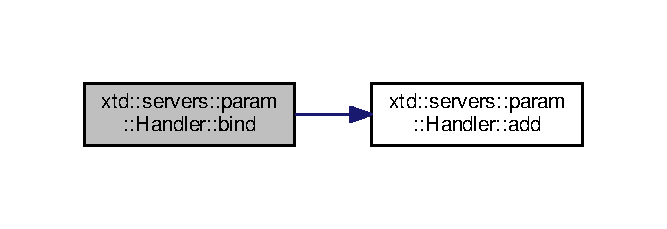
\includegraphics[width=318pt]{classxtd_1_1servers_1_1param_1_1Handler_a3bc858ae5bb7b6ce1f4d0a5eb327d17f_cgraph}
\end{center}
\end{figure}


\index{xtd\+::servers\+::param\+::\+Handler@{xtd\+::servers\+::param\+::\+Handler}!constraint@{constraint}}
\index{constraint@{constraint}!xtd\+::servers\+::param\+::\+Handler@{xtd\+::servers\+::param\+::\+Handler}}
\subsubsection[{\texorpdfstring{constraint(const string \&p\+\_\+name, T p\+\_\+handler)}{constraint(const string &p_name, T p_handler)}}]{\setlength{\rightskip}{0pt plus 5cm}template$<$typename T $>$ bool xtd\+::servers\+::param\+::\+Handler\+::constraint (
\begin{DoxyParamCaption}
\item[{const string \&}]{p\+\_\+name, }
\item[{T}]{p\+\_\+handler}
\end{DoxyParamCaption}
)}\hypertarget{classxtd_1_1servers_1_1param_1_1Handler_a20d689629d4748c14e4a516580a7c55a}{}\label{classxtd_1_1servers_1_1param_1_1Handler_a20d689629d4748c14e4a516580a7c55a}


Add a specific constraint to match while trying to modify a parameter. 

Each time a modification is requested, the constraint will be checked Many constraints can be added, they will be checked in declaration order Opposite constraints must be avoided


\begin{DoxyParams}{Parameters}
{\em p\+\_\+name} & the parameter name \\
\hline
{\em p\+\_\+handler} & the specific constraint \\
\hline
\end{DoxyParams}
\begin{DoxyReturn}{Returns}
true if add succeeds 
\end{DoxyReturn}


Definition at line 245 of file Handler.\+hh.


\begin{DoxyCode}
246 \{
247   t\_params::iterator c\_param = \hyperlink{classxtd_1_1servers_1_1param_1_1Handler_a66465c7a1ee0978f7558d55bfd8bd583}{find}(p\_name);
248 
249   \textcolor{keywordflow}{if} (c\_param == m\_params.end())
250     \textcolor{keywordflow}{return} \textcolor{keyword}{false};
251 
252   c\_param->second->constraint(p\_handler);
253   \textcolor{keywordflow}{return} \textcolor{keyword}{true};
254 \}
\end{DoxyCode}


Here is the call graph for this function\+:
\nopagebreak
\begin{figure}[H]
\begin{center}
\leavevmode
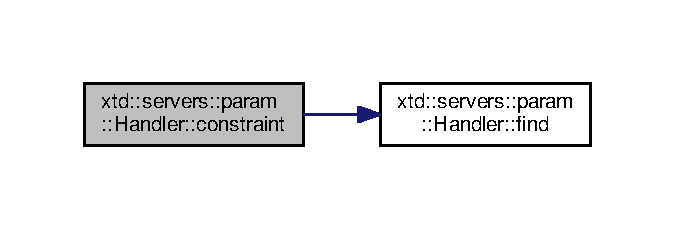
\includegraphics[width=322pt]{classxtd_1_1servers_1_1param_1_1Handler_a20d689629d4748c14e4a516580a7c55a_cgraph}
\end{center}
\end{figure}


\index{xtd\+::servers\+::param\+::\+Handler@{xtd\+::servers\+::param\+::\+Handler}!exists@{exists}}
\index{exists@{exists}!xtd\+::servers\+::param\+::\+Handler@{xtd\+::servers\+::param\+::\+Handler}}
\subsubsection[{\texorpdfstring{exists(const string \&p\+\_\+name)}{exists(const string &p_name)}}]{\setlength{\rightskip}{0pt plus 5cm}bool xtd\+::servers\+::param\+::\+Handler\+::exists (
\begin{DoxyParamCaption}
\item[{const string \&}]{p\+\_\+name}
\end{DoxyParamCaption}
)}\hypertarget{classxtd_1_1servers_1_1param_1_1Handler_a0fcbef276a961d96584354588fc3bfcf}{}\label{classxtd_1_1servers_1_1param_1_1Handler_a0fcbef276a961d96584354588fc3bfcf}


Existency checking. 

N/A


\begin{DoxyParams}{Parameters}
{\em p\+\_\+name} & the parameter to check \\
\hline
\end{DoxyParams}
\begin{DoxyReturn}{Returns}
true if already declared 
\end{DoxyReturn}


Definition at line 89 of file Handler.\+cc.


\begin{DoxyCode}
90 \{
91   \textcolor{keywordflow}{return} (\hyperlink{classxtd_1_1servers_1_1param_1_1Handler_a66465c7a1ee0978f7558d55bfd8bd583}{find}(p\_name) != m\_params.end());
92 \}
\end{DoxyCode}


Here is the call graph for this function\+:
\nopagebreak
\begin{figure}[H]
\begin{center}
\leavevmode
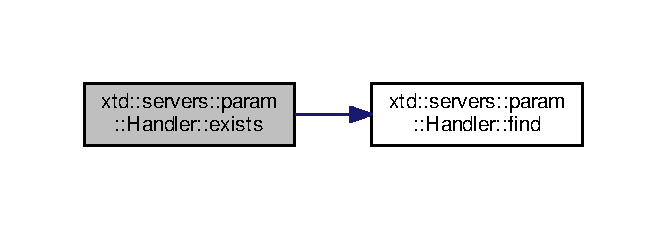
\includegraphics[width=318pt]{classxtd_1_1servers_1_1param_1_1Handler_a0fcbef276a961d96584354588fc3bfcf_cgraph}
\end{center}
\end{figure}


\index{xtd\+::servers\+::param\+::\+Handler@{xtd\+::servers\+::param\+::\+Handler}!find@{find}}
\index{find@{find}!xtd\+::servers\+::param\+::\+Handler@{xtd\+::servers\+::param\+::\+Handler}}
\subsubsection[{\texorpdfstring{find(const string \&p\+\_\+name)}{find(const string &p_name)}}]{\setlength{\rightskip}{0pt plus 5cm}Handler\+::t\+\_\+params\+::iterator xtd\+::servers\+::param\+::\+Handler\+::find (
\begin{DoxyParamCaption}
\item[{const string \&}]{p\+\_\+name}
\end{DoxyParamCaption}
)}\hypertarget{classxtd_1_1servers_1_1param_1_1Handler_a66465c7a1ee0978f7558d55bfd8bd583}{}\label{classxtd_1_1servers_1_1param_1_1Handler_a66465c7a1ee0978f7558d55bfd8bd583}


return an iterator on a find call on map 

make a find with lowercase on given name


\begin{DoxyParams}{Parameters}
{\em p\+\_\+name} & the parameter name to find in map\\
\hline
\end{DoxyParams}
\begin{DoxyReturn}{Returns}
iterator result of map search 
\end{DoxyReturn}


Definition at line 143 of file Handler.\+cc.


\begin{DoxyCode}
144 \{
145   \textcolor{keywordtype}{string} l\_lowerName = p\_name;
146   boost::algorithm::to\_lower(l\_lowerName);
147   \textcolor{keywordflow}{return} m\_params.find(l\_lowerName);
148 \}
\end{DoxyCode}


Here is the caller graph for this function\+:
\nopagebreak
\begin{figure}[H]
\begin{center}
\leavevmode
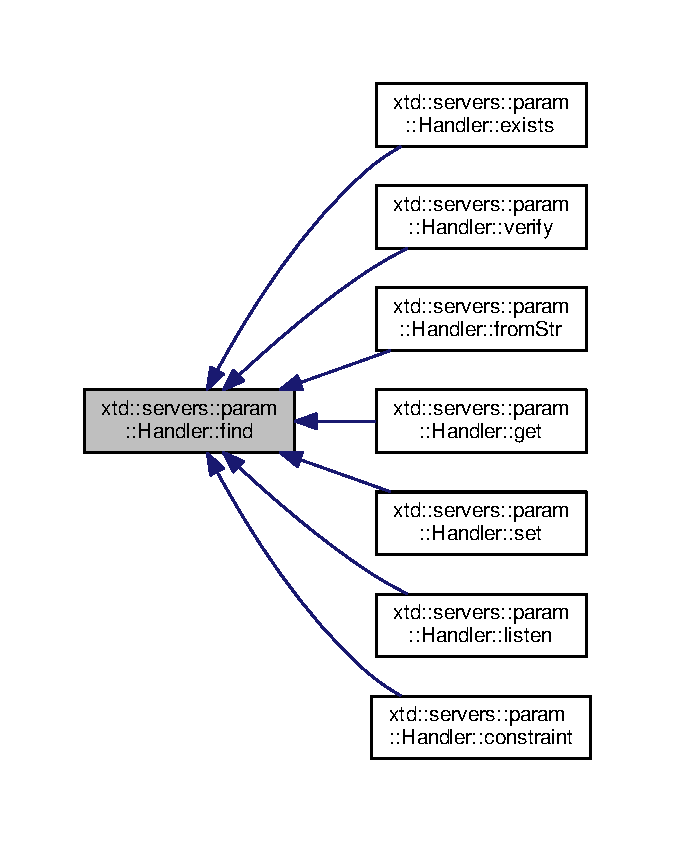
\includegraphics[width=322pt]{classxtd_1_1servers_1_1param_1_1Handler_a66465c7a1ee0978f7558d55bfd8bd583_icgraph}
\end{center}
\end{figure}


\index{xtd\+::servers\+::param\+::\+Handler@{xtd\+::servers\+::param\+::\+Handler}!from\+Str@{from\+Str}}
\index{from\+Str@{from\+Str}!xtd\+::servers\+::param\+::\+Handler@{xtd\+::servers\+::param\+::\+Handler}}
\subsubsection[{\texorpdfstring{from\+Str(const string \&p\+\_\+name, const string \&p\+\_\+src, const string \&p\+\_\+log)}{fromStr(const string &p_name, const string &p_src, const string &p_log)}}]{\setlength{\rightskip}{0pt plus 5cm}bool xtd\+::servers\+::param\+::\+Handler\+::from\+Str (
\begin{DoxyParamCaption}
\item[{const string \&}]{p\+\_\+name, }
\item[{const string \&}]{p\+\_\+src, }
\item[{const string \&}]{p\+\_\+log}
\end{DoxyParamCaption}
)}\hypertarget{classxtd_1_1servers_1_1param_1_1Handler_ab3a53b8db70cf25c3e1de6425d876c37}{}\label{classxtd_1_1servers_1_1param_1_1Handler_ab3a53b8db70cf25c3e1de6425d876c37}


Retreive parameter value from a string. 


\begin{DoxyParams}{Parameters}
{\em p\+\_\+name} & the parameter name \\
\hline
{\em p\+\_\+src} & the string value \\
\hline
{\em p\+\_\+log} & logging message \\
\hline
\end{DoxyParams}
\begin{DoxyReturn}{Returns}
true if it succeeds
\end{DoxyReturn}
N/A 

Definition at line 104 of file Handler.\+cc.


\begin{DoxyCode}
105 \{
106   \textcolor{keywordtype}{bool} l\_ret = \textcolor{keyword}{false};
107   t\_params::iterator c\_param = \hyperlink{classxtd_1_1servers_1_1param_1_1Handler_a66465c7a1ee0978f7558d55bfd8bd583}{find}(p\_name);
108   \textcolor{keywordflow}{if} (c\_param != m\_params.end())
109   \{
110     \textcolor{keywordflow}{if}((l\_ret = c\_param->second->fromStr(p\_src)))
111     \{
112       c\_param->second->setLog(p\_log);
113     \}
114   \}
115   \textcolor{keywordflow}{return} l\_ret;
116 \}
\end{DoxyCode}


Here is the call graph for this function\+:
\nopagebreak
\begin{figure}[H]
\begin{center}
\leavevmode
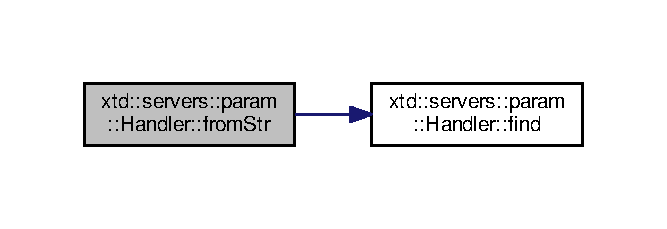
\includegraphics[width=318pt]{classxtd_1_1servers_1_1param_1_1Handler_ab3a53b8db70cf25c3e1de6425d876c37_cgraph}
\end{center}
\end{figure}


\index{xtd\+::servers\+::param\+::\+Handler@{xtd\+::servers\+::param\+::\+Handler}!get@{get}}
\index{get@{get}!xtd\+::servers\+::param\+::\+Handler@{xtd\+::servers\+::param\+::\+Handler}}
\subsubsection[{\texorpdfstring{get(const string \&p\+\_\+name, T \&p\+\_\+dst)}{get(const string &p_name, T &p_dst)}}]{\setlength{\rightskip}{0pt plus 5cm}template$<$typename T $>$ bool xtd\+::servers\+::param\+::\+Handler\+::get (
\begin{DoxyParamCaption}
\item[{const string \&}]{p\+\_\+name, }
\item[{T \&}]{p\+\_\+dst}
\end{DoxyParamCaption}
)}\hypertarget{classxtd_1_1servers_1_1param_1_1Handler_a0f767078fd33fec21e1677d0a0195d8e}{}\label{classxtd_1_1servers_1_1param_1_1Handler_a0f767078fd33fec21e1677d0a0195d8e}


Get the current value of a parameter. 

N/A


\begin{DoxyParams}{Parameters}
{\em p\+\_\+name} & the parameter name \\
\hline
{\em p\+\_\+dst} & the variable to store the content of the current value \\
\hline
\end{DoxyParams}
\begin{DoxyReturn}{Returns}
true if it succeeds 
\end{DoxyReturn}


Definition at line 207 of file Handler.\+hh.


\begin{DoxyCode}
208 \{
209   t\_params::iterator c\_param = \hyperlink{classxtd_1_1servers_1_1param_1_1Handler_a66465c7a1ee0978f7558d55bfd8bd583}{find}(p\_name);
210 
211   \textcolor{keywordflow}{if} (c\_param == m\_params.end())
212     \textcolor{keywordflow}{return} \textcolor{keyword}{false};
213   \textcolor{keywordflow}{return} c\_param->second->get(p\_dst);
214 \}
\end{DoxyCode}


Here is the call graph for this function\+:
\nopagebreak
\begin{figure}[H]
\begin{center}
\leavevmode
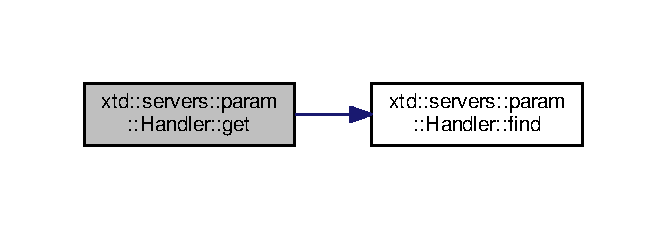
\includegraphics[width=318pt]{classxtd_1_1servers_1_1param_1_1Handler_a0f767078fd33fec21e1677d0a0195d8e_cgraph}
\end{center}
\end{figure}


\index{xtd\+::servers\+::param\+::\+Handler@{xtd\+::servers\+::param\+::\+Handler}!initialize@{initialize}}
\index{initialize@{initialize}!xtd\+::servers\+::param\+::\+Handler@{xtd\+::servers\+::param\+::\+Handler}}
\subsubsection[{\texorpdfstring{initialize(void)}{initialize(void)}}]{\setlength{\rightskip}{0pt plus 5cm}void xtd\+::servers\+::param\+::\+Handler\+::initialize (
\begin{DoxyParamCaption}
\item[{void}]{}
\end{DoxyParamCaption}
)}\hypertarget{classxtd_1_1servers_1_1param_1_1Handler_a9533d788448e6bfdaf1c0f439a9f7b05}{}\label{classxtd_1_1servers_1_1param_1_1Handler_a9533d788448e6bfdaf1c0f439a9f7b05}


Initialization. 

N/A 

Definition at line 47 of file Handler.\+cc.


\begin{DoxyCode}
48 \{
49   \textcolor{keywordflow}{for} (\textcolor{keyword}{auto}& c\_param : m\_params)
50   \{
51     \textcolor{comment}{// Only if parameter is synchronized}
52     \textcolor{keywordflow}{if}(c\_param.second->getSync())
53     \{
54       bfs::path l\_path(m\_actionPath + \textcolor{stringliteral}{"/"} + c\_param.second->getName());
55 
56       \textcolor{keywordflow}{if} (\textcolor{keyword}{false} == is\_regular\_file(l\_path))
57       \{
58         logger::info(\textcolor{stringliteral}{"servers.param.handler"}, \textcolor{stringliteral}{"can't find persistent file to initalize parameter '%s', path
       = %s"}, c\_param.first, l\_path, HERE);
59         c\_param.second->sync();
60       \}
61       \textcolor{keywordflow}{else}
62       \{
63         \textcolor{comment}{// Persistent file found, read value and initialize parameter}
64         ifstream l\_file(l\_path.c\_str());
65         \textcolor{keywordtype}{string}   l\_content;
66 
67         l\_content.assign(std::istreambuf\_iterator<char>(l\_file), std::istreambuf\_iterator<char>());
68         l\_file.close();
69         \textcolor{keywordflow}{if} (\textcolor{keyword}{false} == c\_param.second->fromStr(l\_content))
70           logger::crit(\textcolor{stringliteral}{"servers.param.handler"}, \textcolor{stringliteral}{"unable to initialize param '%s' from value '%s'"}, c\_param.
      first, l\_content, HERE);
71       \}
72     \}
73   \}
74 \}
\end{DoxyCode}


Here is the call graph for this function\+:
\nopagebreak
\begin{figure}[H]
\begin{center}
\leavevmode
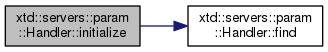
\includegraphics[width=318pt]{classxtd_1_1servers_1_1param_1_1Handler_a9533d788448e6bfdaf1c0f439a9f7b05_cgraph}
\end{center}
\end{figure}


\index{xtd\+::servers\+::param\+::\+Handler@{xtd\+::servers\+::param\+::\+Handler}!listen@{listen}}
\index{listen@{listen}!xtd\+::servers\+::param\+::\+Handler@{xtd\+::servers\+::param\+::\+Handler}}
\subsubsection[{\texorpdfstring{listen(const string \&p\+\_\+name, T p\+\_\+handler)}{listen(const string &p_name, T p_handler)}}]{\setlength{\rightskip}{0pt plus 5cm}template$<$typename T $>$ bool xtd\+::servers\+::param\+::\+Handler\+::listen (
\begin{DoxyParamCaption}
\item[{const string \&}]{p\+\_\+name, }
\item[{T}]{p\+\_\+handler}
\end{DoxyParamCaption}
)}\hypertarget{classxtd_1_1servers_1_1param_1_1Handler_a3e71b80a00c962a862c1d3cc4d623c05}{}\label{classxtd_1_1servers_1_1param_1_1Handler_a3e71b80a00c962a862c1d3cc4d623c05}


Specify the setter to modify the parameter. 

N/A


\begin{DoxyParams}{Parameters}
{\em p\+\_\+name} & the parameter name \\
\hline
{\em p\+\_\+handler} & the modification handler \\
\hline
\end{DoxyParams}
\begin{DoxyReturn}{Returns}
true if it succeeds (i.\+e. parameter exists) 
\end{DoxyReturn}


Definition at line 231 of file Handler.\+hh.


\begin{DoxyCode}
232 \{
233   t\_params::iterator c\_param = \hyperlink{classxtd_1_1servers_1_1param_1_1Handler_a66465c7a1ee0978f7558d55bfd8bd583}{find}(p\_name);
234 
235   \textcolor{keywordflow}{if} (c\_param == m\_params.end())
236     \textcolor{keywordflow}{return} \textcolor{keyword}{false};
237 
238   c\_param->second->listen(p\_handler);
239   \textcolor{keywordflow}{return} \textcolor{keyword}{true};
240 \}
\end{DoxyCode}


Here is the call graph for this function\+:
\nopagebreak
\begin{figure}[H]
\begin{center}
\leavevmode
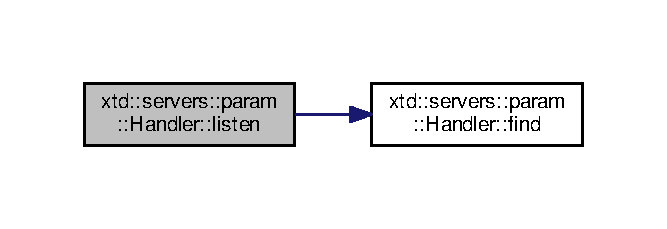
\includegraphics[width=318pt]{classxtd_1_1servers_1_1param_1_1Handler_a3e71b80a00c962a862c1d3cc4d623c05_cgraph}
\end{center}
\end{figure}


\index{xtd\+::servers\+::param\+::\+Handler@{xtd\+::servers\+::param\+::\+Handler}!set@{set}}
\index{set@{set}!xtd\+::servers\+::param\+::\+Handler@{xtd\+::servers\+::param\+::\+Handler}}
\subsubsection[{\texorpdfstring{set(const string \&p\+\_\+name, const T \&p\+\_\+src)}{set(const string &p_name, const T &p_src)}}]{\setlength{\rightskip}{0pt plus 5cm}template$<$typename T $>$ bool xtd\+::servers\+::param\+::\+Handler\+::set (
\begin{DoxyParamCaption}
\item[{const string \&}]{p\+\_\+name, }
\item[{const T \&}]{p\+\_\+src}
\end{DoxyParamCaption}
)}\hypertarget{classxtd_1_1servers_1_1param_1_1Handler_af8dbec0f2d639d39fb11605609462dee}{}\label{classxtd_1_1servers_1_1param_1_1Handler_af8dbec0f2d639d39fb11605609462dee}


Set a parameter value. 

N/A


\begin{DoxyParams}{Parameters}
{\em p\+\_\+name} & the parameter name \\
\hline
{\em p\+\_\+src} & the new value \\
\hline
\end{DoxyParams}
\begin{DoxyReturn}{Returns}
true if it succeeds 
\end{DoxyReturn}


Definition at line 219 of file Handler.\+hh.


\begin{DoxyCode}
220 \{
221   t\_params::iterator c\_param = \hyperlink{classxtd_1_1servers_1_1param_1_1Handler_a66465c7a1ee0978f7558d55bfd8bd583}{find}(p\_name);
222 
223   \textcolor{keywordflow}{if} (c\_param == m\_params.end())
224     \textcolor{keywordflow}{return} \textcolor{keyword}{false};
225   \textcolor{keywordflow}{return} c\_param->second->set(p\_src);
226 \}
\end{DoxyCode}


Here is the call graph for this function\+:
\nopagebreak
\begin{figure}[H]
\begin{center}
\leavevmode
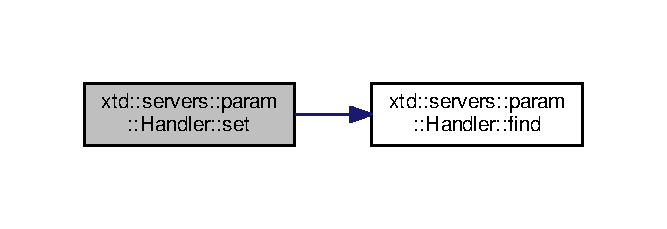
\includegraphics[width=318pt]{classxtd_1_1servers_1_1param_1_1Handler_af8dbec0f2d639d39fb11605609462dee_cgraph}
\end{center}
\end{figure}


\index{xtd\+::servers\+::param\+::\+Handler@{xtd\+::servers\+::param\+::\+Handler}!verify@{verify}}
\index{verify@{verify}!xtd\+::servers\+::param\+::\+Handler@{xtd\+::servers\+::param\+::\+Handler}}
\subsubsection[{\texorpdfstring{verify(const string \&p\+\_\+name, const string \&p\+\_\+src)}{verify(const string &p_name, const string &p_src)}}]{\setlength{\rightskip}{0pt plus 5cm}bool xtd\+::servers\+::param\+::\+Handler\+::verify (
\begin{DoxyParamCaption}
\item[{const string \&}]{p\+\_\+name, }
\item[{const string \&}]{p\+\_\+src}
\end{DoxyParamCaption}
)}\hypertarget{classxtd_1_1servers_1_1param_1_1Handler_aa2b60f898a67bd55c4289686591a2f3b}{}\label{classxtd_1_1servers_1_1param_1_1Handler_aa2b60f898a67bd55c4289686591a2f3b}


Function to verify if given string value can be setted on parameter. 


\begin{DoxyParams}{Parameters}
{\em p\+\_\+name} & parameter value \\
\hline
{\em p\+\_\+src} & the new value \\
\hline
\end{DoxyParams}
\begin{DoxyReturn}{Returns}
true if value can be setted
\end{DoxyReturn}
N/A 

Definition at line 95 of file Handler.\+cc.


\begin{DoxyCode}
96 \{
97   t\_params::iterator c\_param = \hyperlink{classxtd_1_1servers_1_1param_1_1Handler_a66465c7a1ee0978f7558d55bfd8bd583}{find}(p\_name);
98   \textcolor{keywordflow}{if} (c\_param == m\_params.end())
99     \textcolor{keywordflow}{return} \textcolor{keyword}{false};
100   \textcolor{keywordflow}{return} c\_param->second->verify(p\_src);
101 \}
\end{DoxyCode}


Here is the call graph for this function\+:
\nopagebreak
\begin{figure}[H]
\begin{center}
\leavevmode
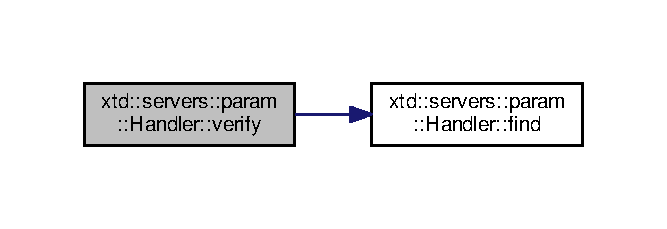
\includegraphics[width=318pt]{classxtd_1_1servers_1_1param_1_1Handler_aa2b60f898a67bd55c4289686591a2f3b_cgraph}
\end{center}
\end{figure}




The documentation for this class was generated from the following files\+:\begin{DoxyCompactItemize}
\item 
/home/psyco/dev/xtdcpp/servers/src/param/\hyperlink{Handler_8hh}{Handler.\+hh}\item 
/home/psyco/dev/xtdcpp/servers/src/param/\hyperlink{Handler_8cc}{Handler.\+cc}\end{DoxyCompactItemize}

\hypertarget{classxtd_1_1servers_1_1app_1_1HtmlOArchive}{}\section{xtd\+:\+:servers\+:\+:app\+:\+:Html\+O\+Archive Class Reference}
\label{classxtd_1_1servers_1_1app_1_1HtmlOArchive}\index{xtd\+::servers\+::app\+::\+Html\+O\+Archive@{xtd\+::servers\+::app\+::\+Html\+O\+Archive}}


{\ttfamily \#include $<$Html\+O\+Archive.\+hh$>$}



Inheritance diagram for xtd\+:\+:servers\+:\+:app\+:\+:Html\+O\+Archive\+:
\nopagebreak
\begin{figure}[H]
\begin{center}
\leavevmode
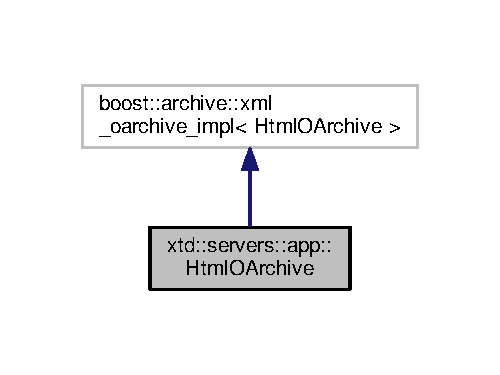
\includegraphics[width=241pt]{classxtd_1_1servers_1_1app_1_1HtmlOArchive__inherit__graph}
\end{center}
\end{figure}


Collaboration diagram for xtd\+:\+:servers\+:\+:app\+:\+:Html\+O\+Archive\+:
\nopagebreak
\begin{figure}[H]
\begin{center}
\leavevmode
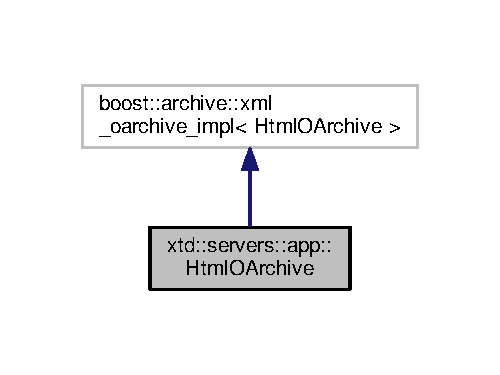
\includegraphics[width=241pt]{classxtd_1_1servers_1_1app_1_1HtmlOArchive__coll__graph}
\end{center}
\end{figure}
\subsection*{Public Types}
\begin{DoxyCompactItemize}
\item 
typedef std\+::stack$<$ context $>$ \hyperlink{classxtd_1_1servers_1_1app_1_1HtmlOArchive_aedb461454d0c255709664fcccc379cf5}{t\+\_\+info}
\item 
typedef std\+::stack$<$ Object $\ast$ $>$ \hyperlink{classxtd_1_1servers_1_1app_1_1HtmlOArchive_a0409a4336819121b7ec0d402ffca9cdf}{t\+\_\+objects}
\end{DoxyCompactItemize}
\subsection*{Public Member Functions}
\begin{DoxyCompactItemize}
\item 
{\footnotesize template$<$class T $>$ }\\\hyperlink{classxtd_1_1servers_1_1app_1_1HtmlOArchive}{Html\+O\+Archive} \& \hyperlink{classxtd_1_1servers_1_1app_1_1HtmlOArchive_ae016000cf5b06b408aa4bfd37c6b354c}{operator$\ast$} (T \&p\+\_\+value)
\item 
{\footnotesize template$<$class T $>$ }\\\hyperlink{classxtd_1_1servers_1_1app_1_1HtmlOArchive}{Html\+O\+Archive} \& \hyperlink{classxtd_1_1servers_1_1app_1_1HtmlOArchive_a5d77d1300bbdbd5e52fec866860bc817}{operator/} (T \&p\+\_\+value)
\item 
void \hyperlink{classxtd_1_1servers_1_1app_1_1HtmlOArchive_a2e5b0b22cf26a77dd62c328a9e51c06f}{save\+\_\+binary} (void $\ast$address, size\+\_\+t count)
\item 
void \hyperlink{classxtd_1_1servers_1_1app_1_1HtmlOArchive_a8675544faff21c5a5acd0af123b48d6d}{save\+\_\+start} (const char $\ast$p\+\_\+name)
\item 
void \hyperlink{classxtd_1_1servers_1_1app_1_1HtmlOArchive_ac5013b8fe0cab7d5c9d7ce3aa4549285}{save\+\_\+end} (const char $\ast$p\+\_\+name)
\item 
{\footnotesize template$<$class T $>$ }\\void \hyperlink{classxtd_1_1servers_1_1app_1_1HtmlOArchive_ace3d9830281bb02de4b775b1ec9891a4}{save\+\_\+override} (T \&t, B\+O\+O\+S\+T\+\_\+\+P\+F\+TO int)
\item 
{\footnotesize template$<$class T $>$ }\\void \hyperlink{classxtd_1_1servers_1_1app_1_1HtmlOArchive_a05042a771dbeccf101cfa84f170f9f85}{save\+\_\+override} (const boost\+::serialization\+::nvp$<$ T $>$ \&t, int)
\item 
{\footnotesize template$<$class T $>$ }\\void \hyperlink{classxtd_1_1servers_1_1app_1_1HtmlOArchive_abde3d494192429180da751c92e31dc63}{save\+\_\+override} (const boost\+::serialization\+::nvp$<$ vector$<$ T $>$ $>$ \&t, int)
\item 
{\footnotesize template$<$class T $>$ }\\void \hyperlink{classxtd_1_1servers_1_1app_1_1HtmlOArchive_ae389e1d1af8f9e39956617521cfefa5e}{save\+\_\+override} (const boost\+::serialization\+::nvp$<$ std\+::deque$<$ T $>$ $>$ \&t, int)
\item 
{\footnotesize template$<$class T $>$ }\\void \hyperlink{classxtd_1_1servers_1_1app_1_1HtmlOArchive_a629a5c1bd96df5f295be173e4f62883e}{save\+\_\+override} (const boost\+::serialization\+::nvp$<$ std\+::list$<$ T $>$ $>$ \&t, int)
\item 
void \hyperlink{classxtd_1_1servers_1_1app_1_1HtmlOArchive_a25bc0aa46ecbc81d01e50e318d85136f}{save} (const char $\ast$)
\item 
void \hyperlink{classxtd_1_1servers_1_1app_1_1HtmlOArchive_ab4a02b5763b656039665add3da76d56f}{save} (const string \&)
\item 
void \hyperlink{classxtd_1_1servers_1_1app_1_1HtmlOArchive_ac34aa74161df424b2a19e41b0c405c25}{save} (const unsigned char \&)
\item 
void \hyperlink{classxtd_1_1servers_1_1app_1_1HtmlOArchive_ac86a79783a5ca046d5eda24a9e6fc558}{save} (const unsigned short \&)
\item 
void \hyperlink{classxtd_1_1servers_1_1app_1_1HtmlOArchive_a5d426b7d61941d71ca43730cdb055055}{save} (const unsigned int \&)
\item 
void \hyperlink{classxtd_1_1servers_1_1app_1_1HtmlOArchive_a4082468458d3b4966bb75d4b92f0d476}{save} (const unsigned long \&)
\item 
void \hyperlink{classxtd_1_1servers_1_1app_1_1HtmlOArchive_a146b049587fa8d292fb9f90f3e23f59b}{save} (const unsigned long long \&)
\item 
void \hyperlink{classxtd_1_1servers_1_1app_1_1HtmlOArchive_a70c1e6b78feb34413275e208fd043964}{save} (const char \&)
\item 
void \hyperlink{classxtd_1_1servers_1_1app_1_1HtmlOArchive_a7dd264fc7222a8689764f4d8ab5c033b}{save} (const short \&)
\item 
void \hyperlink{classxtd_1_1servers_1_1app_1_1HtmlOArchive_af94e2907eba4d436906dc61f57459cd3}{save} (const int \&)
\item 
void \hyperlink{classxtd_1_1servers_1_1app_1_1HtmlOArchive_a2e99b889f990c3fa26b24b6ca1684265}{save} (const long \&)
\item 
void \hyperlink{classxtd_1_1servers_1_1app_1_1HtmlOArchive_addee578d18549c53b00e4c676a568c25}{save} (const long long \&)
\item 
void \hyperlink{classxtd_1_1servers_1_1app_1_1HtmlOArchive_a468a544e41a404c35321f89b1d4cb59c}{save} (const bool \&)
\item 
void \hyperlink{classxtd_1_1servers_1_1app_1_1HtmlOArchive_a5e14af7ab3311cf61fafe8b2742e22be}{save} (const double \&)
\item 
void \hyperlink{classxtd_1_1servers_1_1app_1_1HtmlOArchive_ab9f8811eb20eb372e6cabfa328d2ccf6}{save} (const float \&)
\item 
void \hyperlink{classxtd_1_1servers_1_1app_1_1HtmlOArchive_a9029ddca116a4a843ec6668d1bc3fc90}{save} (const boost\+::serialization\+::collection\+\_\+size\+\_\+type \&)
\item 
void \hyperlink{classxtd_1_1servers_1_1app_1_1HtmlOArchive_afae32c6090882adc5a310a9ba9297c12}{save} (const boost\+::serialization\+::item\+\_\+version\+\_\+type \&)
\item 
void \hyperlink{classxtd_1_1servers_1_1app_1_1HtmlOArchive_a0cd8f9056f209afd354f74073436b70e}{save\+\_\+override} (const boost\+::archive\+::object\+\_\+id\+\_\+type \&t, int)
\item 
void \hyperlink{classxtd_1_1servers_1_1app_1_1HtmlOArchive_add8049c6091432811543e5288706c3c9}{save\+\_\+override} (const boost\+::archive\+::object\+\_\+reference\+\_\+type \&, int)
\item 
void \hyperlink{classxtd_1_1servers_1_1app_1_1HtmlOArchive_a1afeaad47abf3aff1f91b5faa94f869b}{save\+\_\+override} (const boost\+::archive\+::version\+\_\+type \&t, int)
\item 
void \hyperlink{classxtd_1_1servers_1_1app_1_1HtmlOArchive_adbb73e26344036aa3c370bd1a133bf70}{save\+\_\+override} (const boost\+::archive\+::class\+\_\+id\+\_\+type \&t, int)
\item 
void \hyperlink{classxtd_1_1servers_1_1app_1_1HtmlOArchive_aa2bce7ac03f460426a47e25463212908}{save\+\_\+override} (const boost\+::archive\+::class\+\_\+id\+\_\+reference\+\_\+type \&, int)
\item 
void \hyperlink{classxtd_1_1servers_1_1app_1_1HtmlOArchive_a10cb86717b8b49afd68e5b6120662ce9}{save\+\_\+override} (const boost\+::archive\+::class\+\_\+id\+\_\+optional\+\_\+type \&t, int)
\item 
void \hyperlink{classxtd_1_1servers_1_1app_1_1HtmlOArchive_a3238b152ed11274e09c1b0c5995b62c6}{save\+\_\+override} (const boost\+::archive\+::class\+\_\+name\+\_\+type \&, int)
\item 
void \hyperlink{classxtd_1_1servers_1_1app_1_1HtmlOArchive_a62245e0fd68d61841e8e8f34922e5588}{save\+\_\+override} (const boost\+::archive\+::tracking\+\_\+type \&t, int)
\item 
\hyperlink{classxtd_1_1servers_1_1app_1_1HtmlOArchive_a7bf5587951c58ae1652bb73143e41fbc}{Html\+O\+Archive} (std\+::ostream \&p\+\_\+stream)
\end{DoxyCompactItemize}
\subsection*{Public Attributes}
\begin{DoxyCompactItemize}
\item 
\hyperlink{classxtd_1_1servers_1_1app_1_1HtmlOArchive_aedb461454d0c255709664fcccc379cf5}{t\+\_\+info} \hyperlink{classxtd_1_1servers_1_1app_1_1HtmlOArchive_a03bd854507f8457a3b5b575203108ff7}{m\+\_\+info}
\item 
\hyperlink{classxtd_1_1servers_1_1app_1_1HtmlOArchive_a0409a4336819121b7ec0d402ffca9cdf}{t\+\_\+objects} \hyperlink{classxtd_1_1servers_1_1app_1_1HtmlOArchive_a69e333ff9b2b0743e14976cfa4afd6d2}{m\+\_\+objects}
\end{DoxyCompactItemize}
\subsection*{Friends}
\begin{DoxyCompactItemize}
\item 
class \hyperlink{classxtd_1_1servers_1_1app_1_1HtmlOArchive_a725f48824bde766dcd0e8049b4df3df0}{boost\+::archive\+::detail\+::interface\+\_\+oarchive$<$ Html\+O\+Archive $>$}
\item 
class \hyperlink{classxtd_1_1servers_1_1app_1_1HtmlOArchive_a350c2afaed5c679f01f1b4e36a6ad91f}{boost\+::archive\+::basic\+\_\+xml\+\_\+oarchive$<$ Html\+O\+Archive $>$}
\item 
class \hyperlink{classxtd_1_1servers_1_1app_1_1HtmlOArchive_aaca003bb8a4fc59424e4025130da4edd}{boost\+::archive\+::save\+\_\+access}
\end{DoxyCompactItemize}


\subsection{Detailed Description}


Definition at line 19 of file Html\+O\+Archive.\+hh.



\subsection{Member Typedef Documentation}
\index{xtd\+::servers\+::app\+::\+Html\+O\+Archive@{xtd\+::servers\+::app\+::\+Html\+O\+Archive}!t\+\_\+info@{t\+\_\+info}}
\index{t\+\_\+info@{t\+\_\+info}!xtd\+::servers\+::app\+::\+Html\+O\+Archive@{xtd\+::servers\+::app\+::\+Html\+O\+Archive}}
\subsubsection[{\texorpdfstring{t\+\_\+info}{t_info}}]{\setlength{\rightskip}{0pt plus 5cm}typedef std\+::stack$<$context$>$ {\bf xtd\+::servers\+::app\+::\+Html\+O\+Archive\+::t\+\_\+info}}\hypertarget{classxtd_1_1servers_1_1app_1_1HtmlOArchive_aedb461454d0c255709664fcccc379cf5}{}\label{classxtd_1_1servers_1_1app_1_1HtmlOArchive_aedb461454d0c255709664fcccc379cf5}


Definition at line 179 of file Html\+O\+Archive.\+hh.

\index{xtd\+::servers\+::app\+::\+Html\+O\+Archive@{xtd\+::servers\+::app\+::\+Html\+O\+Archive}!t\+\_\+objects@{t\+\_\+objects}}
\index{t\+\_\+objects@{t\+\_\+objects}!xtd\+::servers\+::app\+::\+Html\+O\+Archive@{xtd\+::servers\+::app\+::\+Html\+O\+Archive}}
\subsubsection[{\texorpdfstring{t\+\_\+objects}{t_objects}}]{\setlength{\rightskip}{0pt plus 5cm}typedef std\+::stack$<$Object$\ast$$>$ {\bf xtd\+::servers\+::app\+::\+Html\+O\+Archive\+::t\+\_\+objects}}\hypertarget{classxtd_1_1servers_1_1app_1_1HtmlOArchive_a0409a4336819121b7ec0d402ffca9cdf}{}\label{classxtd_1_1servers_1_1app_1_1HtmlOArchive_a0409a4336819121b7ec0d402ffca9cdf}


Definition at line 180 of file Html\+O\+Archive.\+hh.



\subsection{Constructor \& Destructor Documentation}
\index{xtd\+::servers\+::app\+::\+Html\+O\+Archive@{xtd\+::servers\+::app\+::\+Html\+O\+Archive}!Html\+O\+Archive@{Html\+O\+Archive}}
\index{Html\+O\+Archive@{Html\+O\+Archive}!xtd\+::servers\+::app\+::\+Html\+O\+Archive@{xtd\+::servers\+::app\+::\+Html\+O\+Archive}}
\subsubsection[{\texorpdfstring{Html\+O\+Archive(std\+::ostream \&p\+\_\+stream)}{HtmlOArchive(std::ostream &p_stream)}}]{\setlength{\rightskip}{0pt plus 5cm}xtd\+::servers\+::app\+::\+Html\+O\+Archive\+::\+Html\+O\+Archive (
\begin{DoxyParamCaption}
\item[{std\+::ostream \&}]{p\+\_\+stream}
\end{DoxyParamCaption}
)}\hypertarget{classxtd_1_1servers_1_1app_1_1HtmlOArchive_a7bf5587951c58ae1652bb73143e41fbc}{}\label{classxtd_1_1servers_1_1app_1_1HtmlOArchive_a7bf5587951c58ae1652bb73143e41fbc}


Definition at line 216 of file Html\+O\+Archive.\+cc.


\begin{DoxyCode}
216                                             :
217   boost::archive::xml\_oarchive\_impl<HtmlOArchive>(p\_stream, boost::archive::no\_header),
218   m\_pass(\textcolor{keyword}{false}),
219   m\_depth(0),
220   m\_os(p\_stream),
221   m\_isVector(\textcolor{keyword}{false})
222 \{
223 \}
\end{DoxyCode}


Here is the caller graph for this function\+:
\nopagebreak
\begin{figure}[H]
\begin{center}
\leavevmode
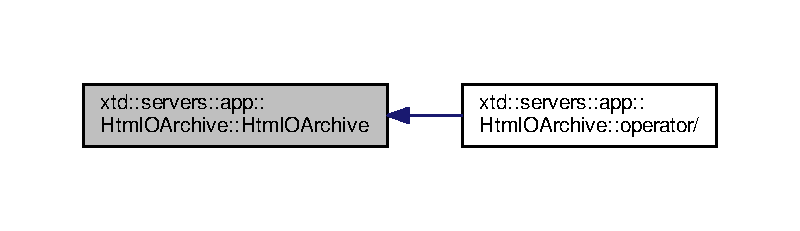
\includegraphics[width=350pt]{classxtd_1_1servers_1_1app_1_1HtmlOArchive_a7bf5587951c58ae1652bb73143e41fbc_icgraph}
\end{center}
\end{figure}




\subsection{Member Function Documentation}
\index{xtd\+::servers\+::app\+::\+Html\+O\+Archive@{xtd\+::servers\+::app\+::\+Html\+O\+Archive}!operator$\ast$@{operator$\ast$}}
\index{operator$\ast$@{operator$\ast$}!xtd\+::servers\+::app\+::\+Html\+O\+Archive@{xtd\+::servers\+::app\+::\+Html\+O\+Archive}}
\subsubsection[{\texorpdfstring{operator$\ast$(\+T \&p\+\_\+value)}{operator*(T &p_value)}}]{\setlength{\rightskip}{0pt plus 5cm}template$<$class T $>$ {\bf Html\+O\+Archive}\& xtd\+::servers\+::app\+::\+Html\+O\+Archive\+::operator$\ast$ (
\begin{DoxyParamCaption}
\item[{T \&}]{p\+\_\+value}
\end{DoxyParamCaption}
)\hspace{0.3cm}{\ttfamily [inline]}}\hypertarget{classxtd_1_1servers_1_1app_1_1HtmlOArchive_ae016000cf5b06b408aa4bfd37c6b354c}{}\label{classxtd_1_1servers_1_1app_1_1HtmlOArchive_ae016000cf5b06b408aa4bfd37c6b354c}


Definition at line 122 of file Html\+O\+Archive.\+hh.


\begin{DoxyCode}
123   \{
124     \textcolor{keywordflow}{return} base::operator&(p\_value);
125   \}
\end{DoxyCode}
\index{xtd\+::servers\+::app\+::\+Html\+O\+Archive@{xtd\+::servers\+::app\+::\+Html\+O\+Archive}!operator/@{operator/}}
\index{operator/@{operator/}!xtd\+::servers\+::app\+::\+Html\+O\+Archive@{xtd\+::servers\+::app\+::\+Html\+O\+Archive}}
\subsubsection[{\texorpdfstring{operator/(\+T \&p\+\_\+value)}{operator/(T &p_value)}}]{\setlength{\rightskip}{0pt plus 5cm}template$<$class T $>$ {\bf Html\+O\+Archive}\& xtd\+::servers\+::app\+::\+Html\+O\+Archive\+::operator/ (
\begin{DoxyParamCaption}
\item[{T \&}]{p\+\_\+value}
\end{DoxyParamCaption}
)\hspace{0.3cm}{\ttfamily [inline]}}\hypertarget{classxtd_1_1servers_1_1app_1_1HtmlOArchive_a5d77d1300bbdbd5e52fec866860bc817}{}\label{classxtd_1_1servers_1_1app_1_1HtmlOArchive_a5d77d1300bbdbd5e52fec866860bc817}


Definition at line 128 of file Html\+O\+Archive.\+hh.


\begin{DoxyCode}
129   \{
130     \textcolor{keywordflow}{return} *\textcolor{keyword}{this} * p\_value;
131   \}
\end{DoxyCode}


Here is the call graph for this function\+:
\nopagebreak
\begin{figure}[H]
\begin{center}
\leavevmode
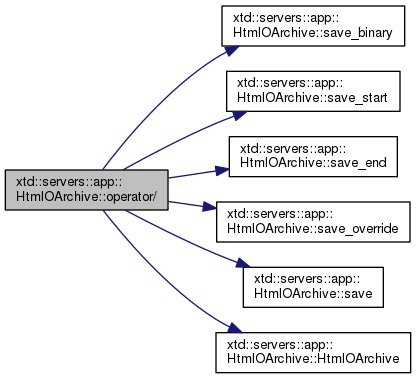
\includegraphics[width=350pt]{classxtd_1_1servers_1_1app_1_1HtmlOArchive_a5d77d1300bbdbd5e52fec866860bc817_cgraph}
\end{center}
\end{figure}


\index{xtd\+::servers\+::app\+::\+Html\+O\+Archive@{xtd\+::servers\+::app\+::\+Html\+O\+Archive}!save@{save}}
\index{save@{save}!xtd\+::servers\+::app\+::\+Html\+O\+Archive@{xtd\+::servers\+::app\+::\+Html\+O\+Archive}}
\subsubsection[{\texorpdfstring{save(const char $\ast$)}{save(const char *)}}]{\setlength{\rightskip}{0pt plus 5cm}void xtd\+::servers\+::app\+::\+Html\+O\+Archive\+::save (
\begin{DoxyParamCaption}
\item[{const char $\ast$}]{t}
\end{DoxyParamCaption}
)}\hypertarget{classxtd_1_1servers_1_1app_1_1HtmlOArchive_a25bc0aa46ecbc81d01e50e318d85136f}{}\label{classxtd_1_1servers_1_1app_1_1HtmlOArchive_a25bc0aa46ecbc81d01e50e318d85136f}


Definition at line 311 of file Html\+O\+Archive.\+cc.


\begin{DoxyCode}
312 \{
313   \hyperlink{classxtd_1_1servers_1_1app_1_1HtmlOArchive_a03bd854507f8457a3b5b575203108ff7}{m\_info}.top().m\_type = \textcolor{stringliteral}{"string"};
314   \textcolor{keywordflow}{if} (0 != t)
315     \hyperlink{classxtd_1_1servers_1_1app_1_1HtmlOArchive_a03bd854507f8457a3b5b575203108ff7}{m\_info}.top().m\_value = string(t);
316 \}
\end{DoxyCode}


Here is the caller graph for this function\+:
\nopagebreak
\begin{figure}[H]
\begin{center}
\leavevmode
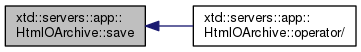
\includegraphics[width=343pt]{classxtd_1_1servers_1_1app_1_1HtmlOArchive_a25bc0aa46ecbc81d01e50e318d85136f_icgraph}
\end{center}
\end{figure}


\index{xtd\+::servers\+::app\+::\+Html\+O\+Archive@{xtd\+::servers\+::app\+::\+Html\+O\+Archive}!save@{save}}
\index{save@{save}!xtd\+::servers\+::app\+::\+Html\+O\+Archive@{xtd\+::servers\+::app\+::\+Html\+O\+Archive}}
\subsubsection[{\texorpdfstring{save(const string \&)}{save(const string &)}}]{\setlength{\rightskip}{0pt plus 5cm}void xtd\+::servers\+::app\+::\+Html\+O\+Archive\+::save (
\begin{DoxyParamCaption}
\item[{const string \&}]{t}
\end{DoxyParamCaption}
)}\hypertarget{classxtd_1_1servers_1_1app_1_1HtmlOArchive_ab4a02b5763b656039665add3da76d56f}{}\label{classxtd_1_1servers_1_1app_1_1HtmlOArchive_ab4a02b5763b656039665add3da76d56f}


Definition at line 319 of file Html\+O\+Archive.\+cc.


\begin{DoxyCode}
320 \{
321   \hyperlink{classxtd_1_1servers_1_1app_1_1HtmlOArchive_a03bd854507f8457a3b5b575203108ff7}{m\_info}.top().m\_type = \textcolor{stringliteral}{"string"};
322   \hyperlink{classxtd_1_1servers_1_1app_1_1HtmlOArchive_a03bd854507f8457a3b5b575203108ff7}{m\_info}.top().m\_value = lexical\_cast<\textcolor{keywordtype}{string}>(t);
323 \}
\end{DoxyCode}
\index{xtd\+::servers\+::app\+::\+Html\+O\+Archive@{xtd\+::servers\+::app\+::\+Html\+O\+Archive}!save@{save}}
\index{save@{save}!xtd\+::servers\+::app\+::\+Html\+O\+Archive@{xtd\+::servers\+::app\+::\+Html\+O\+Archive}}
\subsubsection[{\texorpdfstring{save(const unsigned char \&)}{save(const unsigned char &)}}]{\setlength{\rightskip}{0pt plus 5cm}void xtd\+::servers\+::app\+::\+Html\+O\+Archive\+::save (
\begin{DoxyParamCaption}
\item[{const unsigned char \&}]{t}
\end{DoxyParamCaption}
)}\hypertarget{classxtd_1_1servers_1_1app_1_1HtmlOArchive_ac34aa74161df424b2a19e41b0c405c25}{}\label{classxtd_1_1servers_1_1app_1_1HtmlOArchive_ac34aa74161df424b2a19e41b0c405c25}


Definition at line 326 of file Html\+O\+Archive.\+cc.


\begin{DoxyCode}
327 \{
328   \hyperlink{classxtd_1_1servers_1_1app_1_1HtmlOArchive_a03bd854507f8457a3b5b575203108ff7}{m\_info}.top().m\_type = \textcolor{stringliteral}{"uchar"};
329   \hyperlink{classxtd_1_1servers_1_1app_1_1HtmlOArchive_a03bd854507f8457a3b5b575203108ff7}{m\_info}.top().m\_value = lexical\_cast<\textcolor{keywordtype}{string}>(\textcolor{keyword}{static\_cast<}\textcolor{keywordtype}{unsigned} \textcolor{keywordtype}{int}\textcolor{keyword}{>}(t));
330 \}
\end{DoxyCode}
\index{xtd\+::servers\+::app\+::\+Html\+O\+Archive@{xtd\+::servers\+::app\+::\+Html\+O\+Archive}!save@{save}}
\index{save@{save}!xtd\+::servers\+::app\+::\+Html\+O\+Archive@{xtd\+::servers\+::app\+::\+Html\+O\+Archive}}
\subsubsection[{\texorpdfstring{save(const unsigned short \&)}{save(const unsigned short &)}}]{\setlength{\rightskip}{0pt plus 5cm}void xtd\+::servers\+::app\+::\+Html\+O\+Archive\+::save (
\begin{DoxyParamCaption}
\item[{const unsigned short \&}]{t}
\end{DoxyParamCaption}
)}\hypertarget{classxtd_1_1servers_1_1app_1_1HtmlOArchive_ac86a79783a5ca046d5eda24a9e6fc558}{}\label{classxtd_1_1servers_1_1app_1_1HtmlOArchive_ac86a79783a5ca046d5eda24a9e6fc558}


Definition at line 333 of file Html\+O\+Archive.\+cc.


\begin{DoxyCode}
334 \{
335   \hyperlink{classxtd_1_1servers_1_1app_1_1HtmlOArchive_a03bd854507f8457a3b5b575203108ff7}{m\_info}.top().m\_type = \textcolor{stringliteral}{"ushort"};
336   \hyperlink{classxtd_1_1servers_1_1app_1_1HtmlOArchive_a03bd854507f8457a3b5b575203108ff7}{m\_info}.top().m\_value = lexical\_cast<\textcolor{keywordtype}{string}>(t);
337 \}
\end{DoxyCode}
\index{xtd\+::servers\+::app\+::\+Html\+O\+Archive@{xtd\+::servers\+::app\+::\+Html\+O\+Archive}!save@{save}}
\index{save@{save}!xtd\+::servers\+::app\+::\+Html\+O\+Archive@{xtd\+::servers\+::app\+::\+Html\+O\+Archive}}
\subsubsection[{\texorpdfstring{save(const unsigned int \&)}{save(const unsigned int &)}}]{\setlength{\rightskip}{0pt plus 5cm}void xtd\+::servers\+::app\+::\+Html\+O\+Archive\+::save (
\begin{DoxyParamCaption}
\item[{const unsigned int \&}]{t}
\end{DoxyParamCaption}
)}\hypertarget{classxtd_1_1servers_1_1app_1_1HtmlOArchive_a5d426b7d61941d71ca43730cdb055055}{}\label{classxtd_1_1servers_1_1app_1_1HtmlOArchive_a5d426b7d61941d71ca43730cdb055055}


Definition at line 340 of file Html\+O\+Archive.\+cc.


\begin{DoxyCode}
341 \{
342   \hyperlink{classxtd_1_1servers_1_1app_1_1HtmlOArchive_a03bd854507f8457a3b5b575203108ff7}{m\_info}.top().m\_type = \textcolor{stringliteral}{"uint"};
343   \hyperlink{classxtd_1_1servers_1_1app_1_1HtmlOArchive_a03bd854507f8457a3b5b575203108ff7}{m\_info}.top().m\_value = lexical\_cast<\textcolor{keywordtype}{string}>(t);
344 \}
\end{DoxyCode}
\index{xtd\+::servers\+::app\+::\+Html\+O\+Archive@{xtd\+::servers\+::app\+::\+Html\+O\+Archive}!save@{save}}
\index{save@{save}!xtd\+::servers\+::app\+::\+Html\+O\+Archive@{xtd\+::servers\+::app\+::\+Html\+O\+Archive}}
\subsubsection[{\texorpdfstring{save(const unsigned long \&)}{save(const unsigned long &)}}]{\setlength{\rightskip}{0pt plus 5cm}void xtd\+::servers\+::app\+::\+Html\+O\+Archive\+::save (
\begin{DoxyParamCaption}
\item[{const unsigned long \&}]{t}
\end{DoxyParamCaption}
)}\hypertarget{classxtd_1_1servers_1_1app_1_1HtmlOArchive_a4082468458d3b4966bb75d4b92f0d476}{}\label{classxtd_1_1servers_1_1app_1_1HtmlOArchive_a4082468458d3b4966bb75d4b92f0d476}


Definition at line 347 of file Html\+O\+Archive.\+cc.


\begin{DoxyCode}
348 \{
349   \hyperlink{classxtd_1_1servers_1_1app_1_1HtmlOArchive_a03bd854507f8457a3b5b575203108ff7}{m\_info}.top().m\_type = \textcolor{stringliteral}{"ulong"};
350   \hyperlink{classxtd_1_1servers_1_1app_1_1HtmlOArchive_a03bd854507f8457a3b5b575203108ff7}{m\_info}.top().m\_value = lexical\_cast<\textcolor{keywordtype}{string}>(t);
351 \}
\end{DoxyCode}
\index{xtd\+::servers\+::app\+::\+Html\+O\+Archive@{xtd\+::servers\+::app\+::\+Html\+O\+Archive}!save@{save}}
\index{save@{save}!xtd\+::servers\+::app\+::\+Html\+O\+Archive@{xtd\+::servers\+::app\+::\+Html\+O\+Archive}}
\subsubsection[{\texorpdfstring{save(const unsigned long long \&)}{save(const unsigned long long &)}}]{\setlength{\rightskip}{0pt plus 5cm}void xtd\+::servers\+::app\+::\+Html\+O\+Archive\+::save (
\begin{DoxyParamCaption}
\item[{const unsigned long long \&}]{t}
\end{DoxyParamCaption}
)}\hypertarget{classxtd_1_1servers_1_1app_1_1HtmlOArchive_a146b049587fa8d292fb9f90f3e23f59b}{}\label{classxtd_1_1servers_1_1app_1_1HtmlOArchive_a146b049587fa8d292fb9f90f3e23f59b}


Definition at line 354 of file Html\+O\+Archive.\+cc.


\begin{DoxyCode}
355 \{
356   \hyperlink{classxtd_1_1servers_1_1app_1_1HtmlOArchive_a03bd854507f8457a3b5b575203108ff7}{m\_info}.top().m\_type = \textcolor{stringliteral}{"ulong"};
357   \hyperlink{classxtd_1_1servers_1_1app_1_1HtmlOArchive_a03bd854507f8457a3b5b575203108ff7}{m\_info}.top().m\_value = lexical\_cast<\textcolor{keywordtype}{string}>(t);
358 \}
\end{DoxyCode}
\index{xtd\+::servers\+::app\+::\+Html\+O\+Archive@{xtd\+::servers\+::app\+::\+Html\+O\+Archive}!save@{save}}
\index{save@{save}!xtd\+::servers\+::app\+::\+Html\+O\+Archive@{xtd\+::servers\+::app\+::\+Html\+O\+Archive}}
\subsubsection[{\texorpdfstring{save(const char \&)}{save(const char &)}}]{\setlength{\rightskip}{0pt plus 5cm}void xtd\+::servers\+::app\+::\+Html\+O\+Archive\+::save (
\begin{DoxyParamCaption}
\item[{const char \&}]{t}
\end{DoxyParamCaption}
)}\hypertarget{classxtd_1_1servers_1_1app_1_1HtmlOArchive_a70c1e6b78feb34413275e208fd043964}{}\label{classxtd_1_1servers_1_1app_1_1HtmlOArchive_a70c1e6b78feb34413275e208fd043964}


Definition at line 361 of file Html\+O\+Archive.\+cc.


\begin{DoxyCode}
362 \{
363   \hyperlink{classxtd_1_1servers_1_1app_1_1HtmlOArchive_a03bd854507f8457a3b5b575203108ff7}{m\_info}.top().m\_type = \textcolor{stringliteral}{"schar"};
364   \hyperlink{classxtd_1_1servers_1_1app_1_1HtmlOArchive_a03bd854507f8457a3b5b575203108ff7}{m\_info}.top().m\_value = lexical\_cast<\textcolor{keywordtype}{string}>(\textcolor{keyword}{static\_cast<}\textcolor{keywordtype}{int}\textcolor{keyword}{>}(t));
365 \}
\end{DoxyCode}
\index{xtd\+::servers\+::app\+::\+Html\+O\+Archive@{xtd\+::servers\+::app\+::\+Html\+O\+Archive}!save@{save}}
\index{save@{save}!xtd\+::servers\+::app\+::\+Html\+O\+Archive@{xtd\+::servers\+::app\+::\+Html\+O\+Archive}}
\subsubsection[{\texorpdfstring{save(const short \&)}{save(const short &)}}]{\setlength{\rightskip}{0pt plus 5cm}void xtd\+::servers\+::app\+::\+Html\+O\+Archive\+::save (
\begin{DoxyParamCaption}
\item[{const short \&}]{t}
\end{DoxyParamCaption}
)}\hypertarget{classxtd_1_1servers_1_1app_1_1HtmlOArchive_a7dd264fc7222a8689764f4d8ab5c033b}{}\label{classxtd_1_1servers_1_1app_1_1HtmlOArchive_a7dd264fc7222a8689764f4d8ab5c033b}


Definition at line 368 of file Html\+O\+Archive.\+cc.


\begin{DoxyCode}
369 \{
370   \hyperlink{classxtd_1_1servers_1_1app_1_1HtmlOArchive_a03bd854507f8457a3b5b575203108ff7}{m\_info}.top().m\_type = \textcolor{stringliteral}{"sshort"};
371   \hyperlink{classxtd_1_1servers_1_1app_1_1HtmlOArchive_a03bd854507f8457a3b5b575203108ff7}{m\_info}.top().m\_value = lexical\_cast<\textcolor{keywordtype}{string}>(t);
372 \}
\end{DoxyCode}
\index{xtd\+::servers\+::app\+::\+Html\+O\+Archive@{xtd\+::servers\+::app\+::\+Html\+O\+Archive}!save@{save}}
\index{save@{save}!xtd\+::servers\+::app\+::\+Html\+O\+Archive@{xtd\+::servers\+::app\+::\+Html\+O\+Archive}}
\subsubsection[{\texorpdfstring{save(const int \&)}{save(const int &)}}]{\setlength{\rightskip}{0pt plus 5cm}void xtd\+::servers\+::app\+::\+Html\+O\+Archive\+::save (
\begin{DoxyParamCaption}
\item[{const int \&}]{t}
\end{DoxyParamCaption}
)}\hypertarget{classxtd_1_1servers_1_1app_1_1HtmlOArchive_af94e2907eba4d436906dc61f57459cd3}{}\label{classxtd_1_1servers_1_1app_1_1HtmlOArchive_af94e2907eba4d436906dc61f57459cd3}


Definition at line 375 of file Html\+O\+Archive.\+cc.


\begin{DoxyCode}
376 \{
377   \hyperlink{classxtd_1_1servers_1_1app_1_1HtmlOArchive_a03bd854507f8457a3b5b575203108ff7}{m\_info}.top().m\_type = \textcolor{stringliteral}{"sint"};
378   \hyperlink{classxtd_1_1servers_1_1app_1_1HtmlOArchive_a03bd854507f8457a3b5b575203108ff7}{m\_info}.top().m\_value = lexical\_cast<\textcolor{keywordtype}{string}>(t);
379 \}
\end{DoxyCode}
\index{xtd\+::servers\+::app\+::\+Html\+O\+Archive@{xtd\+::servers\+::app\+::\+Html\+O\+Archive}!save@{save}}
\index{save@{save}!xtd\+::servers\+::app\+::\+Html\+O\+Archive@{xtd\+::servers\+::app\+::\+Html\+O\+Archive}}
\subsubsection[{\texorpdfstring{save(const long \&)}{save(const long &)}}]{\setlength{\rightskip}{0pt plus 5cm}void xtd\+::servers\+::app\+::\+Html\+O\+Archive\+::save (
\begin{DoxyParamCaption}
\item[{const long \&}]{t}
\end{DoxyParamCaption}
)}\hypertarget{classxtd_1_1servers_1_1app_1_1HtmlOArchive_a2e99b889f990c3fa26b24b6ca1684265}{}\label{classxtd_1_1servers_1_1app_1_1HtmlOArchive_a2e99b889f990c3fa26b24b6ca1684265}


Definition at line 382 of file Html\+O\+Archive.\+cc.


\begin{DoxyCode}
383 \{
384   \hyperlink{classxtd_1_1servers_1_1app_1_1HtmlOArchive_a03bd854507f8457a3b5b575203108ff7}{m\_info}.top().m\_type = \textcolor{stringliteral}{"slong"};
385   \hyperlink{classxtd_1_1servers_1_1app_1_1HtmlOArchive_a03bd854507f8457a3b5b575203108ff7}{m\_info}.top().m\_value = lexical\_cast<\textcolor{keywordtype}{string}>(t);
386 \}
\end{DoxyCode}
\index{xtd\+::servers\+::app\+::\+Html\+O\+Archive@{xtd\+::servers\+::app\+::\+Html\+O\+Archive}!save@{save}}
\index{save@{save}!xtd\+::servers\+::app\+::\+Html\+O\+Archive@{xtd\+::servers\+::app\+::\+Html\+O\+Archive}}
\subsubsection[{\texorpdfstring{save(const long long \&)}{save(const long long &)}}]{\setlength{\rightskip}{0pt plus 5cm}void xtd\+::servers\+::app\+::\+Html\+O\+Archive\+::save (
\begin{DoxyParamCaption}
\item[{const long long \&}]{t}
\end{DoxyParamCaption}
)}\hypertarget{classxtd_1_1servers_1_1app_1_1HtmlOArchive_addee578d18549c53b00e4c676a568c25}{}\label{classxtd_1_1servers_1_1app_1_1HtmlOArchive_addee578d18549c53b00e4c676a568c25}


Definition at line 389 of file Html\+O\+Archive.\+cc.


\begin{DoxyCode}
390 \{
391   \hyperlink{classxtd_1_1servers_1_1app_1_1HtmlOArchive_a03bd854507f8457a3b5b575203108ff7}{m\_info}.top().m\_type = \textcolor{stringliteral}{"slong"};
392   \hyperlink{classxtd_1_1servers_1_1app_1_1HtmlOArchive_a03bd854507f8457a3b5b575203108ff7}{m\_info}.top().m\_value = lexical\_cast<\textcolor{keywordtype}{string}>(t);
393 \}
\end{DoxyCode}
\index{xtd\+::servers\+::app\+::\+Html\+O\+Archive@{xtd\+::servers\+::app\+::\+Html\+O\+Archive}!save@{save}}
\index{save@{save}!xtd\+::servers\+::app\+::\+Html\+O\+Archive@{xtd\+::servers\+::app\+::\+Html\+O\+Archive}}
\subsubsection[{\texorpdfstring{save(const bool \&)}{save(const bool &)}}]{\setlength{\rightskip}{0pt plus 5cm}void xtd\+::servers\+::app\+::\+Html\+O\+Archive\+::save (
\begin{DoxyParamCaption}
\item[{const bool \&}]{t}
\end{DoxyParamCaption}
)}\hypertarget{classxtd_1_1servers_1_1app_1_1HtmlOArchive_a468a544e41a404c35321f89b1d4cb59c}{}\label{classxtd_1_1servers_1_1app_1_1HtmlOArchive_a468a544e41a404c35321f89b1d4cb59c}


Definition at line 396 of file Html\+O\+Archive.\+cc.


\begin{DoxyCode}
397 \{
398   \hyperlink{classxtd_1_1servers_1_1app_1_1HtmlOArchive_a03bd854507f8457a3b5b575203108ff7}{m\_info}.top().m\_type = \textcolor{stringliteral}{"bool"};
399   \textcolor{keywordflow}{if} (t)
400     \hyperlink{classxtd_1_1servers_1_1app_1_1HtmlOArchive_a03bd854507f8457a3b5b575203108ff7}{m\_info}.top().m\_value = \textcolor{stringliteral}{"1"};
401   \textcolor{keywordflow}{else}
402     \hyperlink{classxtd_1_1servers_1_1app_1_1HtmlOArchive_a03bd854507f8457a3b5b575203108ff7}{m\_info}.top().m\_value = \textcolor{stringliteral}{"0"};
403 \}
\end{DoxyCode}
\index{xtd\+::servers\+::app\+::\+Html\+O\+Archive@{xtd\+::servers\+::app\+::\+Html\+O\+Archive}!save@{save}}
\index{save@{save}!xtd\+::servers\+::app\+::\+Html\+O\+Archive@{xtd\+::servers\+::app\+::\+Html\+O\+Archive}}
\subsubsection[{\texorpdfstring{save(const double \&)}{save(const double &)}}]{\setlength{\rightskip}{0pt plus 5cm}void xtd\+::servers\+::app\+::\+Html\+O\+Archive\+::save (
\begin{DoxyParamCaption}
\item[{const double \&}]{t}
\end{DoxyParamCaption}
)}\hypertarget{classxtd_1_1servers_1_1app_1_1HtmlOArchive_a5e14af7ab3311cf61fafe8b2742e22be}{}\label{classxtd_1_1servers_1_1app_1_1HtmlOArchive_a5e14af7ab3311cf61fafe8b2742e22be}


Definition at line 406 of file Html\+O\+Archive.\+cc.


\begin{DoxyCode}
407 \{
408   \hyperlink{classxtd_1_1servers_1_1app_1_1HtmlOArchive_a03bd854507f8457a3b5b575203108ff7}{m\_info}.top().m\_type = \textcolor{stringliteral}{"double"};
409   \hyperlink{classxtd_1_1servers_1_1app_1_1HtmlOArchive_a03bd854507f8457a3b5b575203108ff7}{m\_info}.top().m\_value = lexical\_cast<\textcolor{keywordtype}{string}>(t);
410 \}
\end{DoxyCode}
\index{xtd\+::servers\+::app\+::\+Html\+O\+Archive@{xtd\+::servers\+::app\+::\+Html\+O\+Archive}!save@{save}}
\index{save@{save}!xtd\+::servers\+::app\+::\+Html\+O\+Archive@{xtd\+::servers\+::app\+::\+Html\+O\+Archive}}
\subsubsection[{\texorpdfstring{save(const float \&)}{save(const float &)}}]{\setlength{\rightskip}{0pt plus 5cm}void xtd\+::servers\+::app\+::\+Html\+O\+Archive\+::save (
\begin{DoxyParamCaption}
\item[{const float \&}]{t}
\end{DoxyParamCaption}
)}\hypertarget{classxtd_1_1servers_1_1app_1_1HtmlOArchive_ab9f8811eb20eb372e6cabfa328d2ccf6}{}\label{classxtd_1_1servers_1_1app_1_1HtmlOArchive_ab9f8811eb20eb372e6cabfa328d2ccf6}


Definition at line 413 of file Html\+O\+Archive.\+cc.


\begin{DoxyCode}
414 \{
415   \hyperlink{classxtd_1_1servers_1_1app_1_1HtmlOArchive_a03bd854507f8457a3b5b575203108ff7}{m\_info}.top().m\_type = \textcolor{stringliteral}{"float"};
416   \hyperlink{classxtd_1_1servers_1_1app_1_1HtmlOArchive_a03bd854507f8457a3b5b575203108ff7}{m\_info}.top().m\_value = lexical\_cast<\textcolor{keywordtype}{string}>(t);
417 \}
\end{DoxyCode}
\index{xtd\+::servers\+::app\+::\+Html\+O\+Archive@{xtd\+::servers\+::app\+::\+Html\+O\+Archive}!save@{save}}
\index{save@{save}!xtd\+::servers\+::app\+::\+Html\+O\+Archive@{xtd\+::servers\+::app\+::\+Html\+O\+Archive}}
\subsubsection[{\texorpdfstring{save(const boost\+::serialization\+::collection\+\_\+size\+\_\+type \&)}{save(const boost::serialization::collection_size_type &)}}]{\setlength{\rightskip}{0pt plus 5cm}void xtd\+::servers\+::app\+::\+Html\+O\+Archive\+::save (
\begin{DoxyParamCaption}
\item[{const boost\+::serialization\+::collection\+\_\+size\+\_\+type \&}]{}
\end{DoxyParamCaption}
)}\hypertarget{classxtd_1_1servers_1_1app_1_1HtmlOArchive_a9029ddca116a4a843ec6668d1bc3fc90}{}\label{classxtd_1_1servers_1_1app_1_1HtmlOArchive_a9029ddca116a4a843ec6668d1bc3fc90}


Definition at line 420 of file Html\+O\+Archive.\+cc.


\begin{DoxyCode}
421 \{
422   \textcolor{comment}{//base::save(t);}
423 \}
\end{DoxyCode}
\index{xtd\+::servers\+::app\+::\+Html\+O\+Archive@{xtd\+::servers\+::app\+::\+Html\+O\+Archive}!save@{save}}
\index{save@{save}!xtd\+::servers\+::app\+::\+Html\+O\+Archive@{xtd\+::servers\+::app\+::\+Html\+O\+Archive}}
\subsubsection[{\texorpdfstring{save(const boost\+::serialization\+::item\+\_\+version\+\_\+type \&)}{save(const boost::serialization::item_version_type &)}}]{\setlength{\rightskip}{0pt plus 5cm}void xtd\+::servers\+::app\+::\+Html\+O\+Archive\+::save (
\begin{DoxyParamCaption}
\item[{const boost\+::serialization\+::item\+\_\+version\+\_\+type \&}]{t}
\end{DoxyParamCaption}
)}\hypertarget{classxtd_1_1servers_1_1app_1_1HtmlOArchive_afae32c6090882adc5a310a9ba9297c12}{}\label{classxtd_1_1servers_1_1app_1_1HtmlOArchive_afae32c6090882adc5a310a9ba9297c12}


Definition at line 426 of file Html\+O\+Archive.\+cc.


\begin{DoxyCode}
427 \{
428   \hyperlink{classxtd_1_1servers_1_1app_1_1HtmlOArchive_a03bd854507f8457a3b5b575203108ff7}{m\_info}.top().m\_itemVersion = t;
429 \}
\end{DoxyCode}
\index{xtd\+::servers\+::app\+::\+Html\+O\+Archive@{xtd\+::servers\+::app\+::\+Html\+O\+Archive}!save\+\_\+binary@{save\+\_\+binary}}
\index{save\+\_\+binary@{save\+\_\+binary}!xtd\+::servers\+::app\+::\+Html\+O\+Archive@{xtd\+::servers\+::app\+::\+Html\+O\+Archive}}
\subsubsection[{\texorpdfstring{save\+\_\+binary(void $\ast$address, size\+\_\+t count)}{save_binary(void *address, size_t count)}}]{\setlength{\rightskip}{0pt plus 5cm}void xtd\+::servers\+::app\+::\+Html\+O\+Archive\+::save\+\_\+binary (
\begin{DoxyParamCaption}
\item[{void $\ast$}]{address, }
\item[{size\+\_\+t}]{count}
\end{DoxyParamCaption}
)}\hypertarget{classxtd_1_1servers_1_1app_1_1HtmlOArchive_a2e5b0b22cf26a77dd62c328a9e51c06f}{}\label{classxtd_1_1servers_1_1app_1_1HtmlOArchive_a2e5b0b22cf26a77dd62c328a9e51c06f}


Definition at line 226 of file Html\+O\+Archive.\+cc.


\begin{DoxyCode}
227 \{
228   base::save\_binary(address, count);
229 \}
\end{DoxyCode}


Here is the caller graph for this function\+:
\nopagebreak
\begin{figure}[H]
\begin{center}
\leavevmode
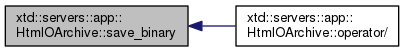
\includegraphics[width=350pt]{classxtd_1_1servers_1_1app_1_1HtmlOArchive_a2e5b0b22cf26a77dd62c328a9e51c06f_icgraph}
\end{center}
\end{figure}


\index{xtd\+::servers\+::app\+::\+Html\+O\+Archive@{xtd\+::servers\+::app\+::\+Html\+O\+Archive}!save\+\_\+end@{save\+\_\+end}}
\index{save\+\_\+end@{save\+\_\+end}!xtd\+::servers\+::app\+::\+Html\+O\+Archive@{xtd\+::servers\+::app\+::\+Html\+O\+Archive}}
\subsubsection[{\texorpdfstring{save\+\_\+end(const char $\ast$p\+\_\+name)}{save_end(const char *p_name)}}]{\setlength{\rightskip}{0pt plus 5cm}void xtd\+::servers\+::app\+::\+Html\+O\+Archive\+::save\+\_\+end (
\begin{DoxyParamCaption}
\item[{const char $\ast$}]{p\+\_\+name}
\end{DoxyParamCaption}
)}\hypertarget{classxtd_1_1servers_1_1app_1_1HtmlOArchive_ac5013b8fe0cab7d5c9d7ce3aa4549285}{}\label{classxtd_1_1servers_1_1app_1_1HtmlOArchive_ac5013b8fe0cab7d5c9d7ce3aa4549285}


Definition at line 251 of file Html\+O\+Archive.\+cc.


\begin{DoxyCode}
252 \{
253   \textcolor{keywordflow}{if} (m\_pass)
254     \textcolor{keywordflow}{return};
255   \textcolor{keywordflow}{if} (0 == p\_name)
256     \textcolor{keywordflow}{return};
257 
258   \textcolor{comment}{//     this->This()->put(str(format("  depth : %s\(\backslash\)n") % m\_info.size()).c\_str());}
259   \textcolor{comment}{//     this->This()->put(str(format("   name : %s\(\backslash\)n") % l\_cur.m\_fieldName).c\_str());}
260   \textcolor{comment}{//     this->This()->put(str(format("classid : %d\(\backslash\)n") % l\_cur.m\_classID).c\_str());}
261   \textcolor{comment}{//     this->This()->put(str(format("  track : %d\(\backslash\)n") % l\_cur.m\_tracking).c\_str());}
262   \textcolor{comment}{//     this->This()->put(str(format("version : %d\(\backslash\)n") % l\_cur.m\_version).c\_str());}
263   \textcolor{comment}{//     this->This()->put(str(format(" object : %d\(\backslash\)n") % l\_cur.m\_objectID).c\_str());}
264   \textcolor{comment}{//     this->This()->put(str(format("   type : %s\(\backslash\)n") % l\_cur.m\_type).c\_str());}
265   \textcolor{comment}{//     this->This()->put("\(\backslash\)n\(\backslash\)n");}
266 
267   \textcolor{keyword}{const} context& l\_cur = \hyperlink{classxtd_1_1servers_1_1app_1_1HtmlOArchive_a03bd854507f8457a3b5b575203108ff7}{m\_info}.top();
268 
269   \textcolor{keywordflow}{if} ((l\_cur.m\_type != \textcolor{stringliteral}{"struct"}) && (l\_cur.m\_type != \textcolor{stringliteral}{"vector"}))
270   \{
271     \hyperlink{classxtd_1_1servers_1_1app_1_1HtmlOArchive_a69e333ff9b2b0743e14976cfa4afd6d2}{m\_objects}.push(\textcolor{keyword}{new} PodObject(l\_cur.m\_fieldName, l\_cur.m\_depth, l\_cur.m\_type, l\_cur.m\_value));
272   \}
273   \textcolor{keywordflow}{else}
274   \{
275     StructObject* l\_new = 0;
276     \textcolor{keywordflow}{if} (l\_cur.m\_type == \textcolor{stringliteral}{"struct"})
277     \{
278       l\_new = \textcolor{keyword}{new} StructObject(l\_cur.m\_fieldName,
279                                l\_cur.m\_depth,
280                                l\_cur.m\_classID,
281                                l\_cur.m\_objectID,
282                                l\_cur.m\_version,
283                                l\_cur.m\_tracking);
284       \textcolor{keywordflow}{while} ((\hyperlink{classxtd_1_1servers_1_1app_1_1HtmlOArchive_a69e333ff9b2b0743e14976cfa4afd6d2}{m\_objects}.size() != 0) && (l\_new->m\_depth < \hyperlink{classxtd_1_1servers_1_1app_1_1HtmlOArchive_a69e333ff9b2b0743e14976cfa4afd6d2}{m\_objects}.top()->m\_depth))
285       \{
286         l\_new->m\_childs.push\_back(\hyperlink{classxtd_1_1servers_1_1app_1_1HtmlOArchive_a69e333ff9b2b0743e14976cfa4afd6d2}{m\_objects}.top());
287         \hyperlink{classxtd_1_1servers_1_1app_1_1HtmlOArchive_a69e333ff9b2b0743e14976cfa4afd6d2}{m\_objects}.pop();
288       \}
289     \}
290     \textcolor{keywordflow}{else}
291     \{
292       l\_new = \textcolor{keyword}{new} VectorObject(l\_cur.m\_fieldName,
293                                l\_cur.m\_depth,
294                                l\_cur.m\_classID,
295                                l\_cur.m\_objectID,
296                                l\_cur.m\_version,
297                                l\_cur.m\_tracking,
298                                l\_cur.m\_itemVersion);
299       \hyperlink{classxtd_1_1servers_1_1app_1_1HtmlOArchive_a69e333ff9b2b0743e14976cfa4afd6d2}{m\_objects}.top()->m\_name = l\_new->m\_name + \textcolor{stringliteral}{"Item"};
300       l\_new->m\_childs.push\_back(\hyperlink{classxtd_1_1servers_1_1app_1_1HtmlOArchive_a69e333ff9b2b0743e14976cfa4afd6d2}{m\_objects}.top());
301       \hyperlink{classxtd_1_1servers_1_1app_1_1HtmlOArchive_a69e333ff9b2b0743e14976cfa4afd6d2}{m\_objects}.pop();
302     \}
303     \hyperlink{classxtd_1_1servers_1_1app_1_1HtmlOArchive_a69e333ff9b2b0743e14976cfa4afd6d2}{m\_objects}.push(l\_new);
304   \}
305 
306   \hyperlink{classxtd_1_1servers_1_1app_1_1HtmlOArchive_a03bd854507f8457a3b5b575203108ff7}{m\_info}.pop();
307 \}
\end{DoxyCode}


Here is the caller graph for this function\+:
\nopagebreak
\begin{figure}[H]
\begin{center}
\leavevmode
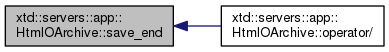
\includegraphics[width=350pt]{classxtd_1_1servers_1_1app_1_1HtmlOArchive_ac5013b8fe0cab7d5c9d7ce3aa4549285_icgraph}
\end{center}
\end{figure}


\index{xtd\+::servers\+::app\+::\+Html\+O\+Archive@{xtd\+::servers\+::app\+::\+Html\+O\+Archive}!save\+\_\+override@{save\+\_\+override}}
\index{save\+\_\+override@{save\+\_\+override}!xtd\+::servers\+::app\+::\+Html\+O\+Archive@{xtd\+::servers\+::app\+::\+Html\+O\+Archive}}
\subsubsection[{\texorpdfstring{save\+\_\+override(\+T \&t, B\+O\+O\+S\+T\+\_\+\+P\+F\+T\+O int)}{save_override(T &t, BOOST_PFTO int)}}]{\setlength{\rightskip}{0pt plus 5cm}template$<$class T $>$ void xtd\+::servers\+::app\+::\+Html\+O\+Archive\+::save\+\_\+override (
\begin{DoxyParamCaption}
\item[{T \&}]{t, }
\item[{B\+O\+O\+S\+T\+\_\+\+P\+F\+TO}]{int}
\end{DoxyParamCaption}
)}\hypertarget{classxtd_1_1servers_1_1app_1_1HtmlOArchive_ace3d9830281bb02de4b775b1ec9891a4}{}\label{classxtd_1_1servers_1_1app_1_1HtmlOArchive_ace3d9830281bb02de4b775b1ec9891a4}


Here is the caller graph for this function\+:
\nopagebreak
\begin{figure}[H]
\begin{center}
\leavevmode
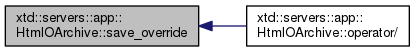
\includegraphics[width=350pt]{classxtd_1_1servers_1_1app_1_1HtmlOArchive_ace3d9830281bb02de4b775b1ec9891a4_icgraph}
\end{center}
\end{figure}


\index{xtd\+::servers\+::app\+::\+Html\+O\+Archive@{xtd\+::servers\+::app\+::\+Html\+O\+Archive}!save\+\_\+override@{save\+\_\+override}}
\index{save\+\_\+override@{save\+\_\+override}!xtd\+::servers\+::app\+::\+Html\+O\+Archive@{xtd\+::servers\+::app\+::\+Html\+O\+Archive}}
\subsubsection[{\texorpdfstring{save\+\_\+override(const boost\+::serialization\+::nvp$<$ T $>$ \&t, int)}{save_override(const boost::serialization::nvp< T > &t, int)}}]{\setlength{\rightskip}{0pt plus 5cm}template$<$class T $>$ void xtd\+::servers\+::app\+::\+Html\+O\+Archive\+::save\+\_\+override (
\begin{DoxyParamCaption}
\item[{const boost\+::serialization\+::nvp$<$ T $>$ \&}]{t, }
\item[{int}]{}
\end{DoxyParamCaption}
)}\hypertarget{classxtd_1_1servers_1_1app_1_1HtmlOArchive_a05042a771dbeccf101cfa84f170f9f85}{}\label{classxtd_1_1servers_1_1app_1_1HtmlOArchive_a05042a771dbeccf101cfa84f170f9f85}
\index{xtd\+::servers\+::app\+::\+Html\+O\+Archive@{xtd\+::servers\+::app\+::\+Html\+O\+Archive}!save\+\_\+override@{save\+\_\+override}}
\index{save\+\_\+override@{save\+\_\+override}!xtd\+::servers\+::app\+::\+Html\+O\+Archive@{xtd\+::servers\+::app\+::\+Html\+O\+Archive}}
\subsubsection[{\texorpdfstring{save\+\_\+override(const boost\+::serialization\+::nvp$<$ vector$<$ T $>$ $>$ \&t, int)}{save_override(const boost::serialization::nvp< vector< T > > &t, int)}}]{\setlength{\rightskip}{0pt plus 5cm}template$<$class T $>$ void xtd\+::servers\+::app\+::\+Html\+O\+Archive\+::save\+\_\+override (
\begin{DoxyParamCaption}
\item[{const boost\+::serialization\+::nvp$<$ vector$<$ T $>$ $>$ \&}]{t, }
\item[{int}]{}
\end{DoxyParamCaption}
)}\hypertarget{classxtd_1_1servers_1_1app_1_1HtmlOArchive_abde3d494192429180da751c92e31dc63}{}\label{classxtd_1_1servers_1_1app_1_1HtmlOArchive_abde3d494192429180da751c92e31dc63}
\index{xtd\+::servers\+::app\+::\+Html\+O\+Archive@{xtd\+::servers\+::app\+::\+Html\+O\+Archive}!save\+\_\+override@{save\+\_\+override}}
\index{save\+\_\+override@{save\+\_\+override}!xtd\+::servers\+::app\+::\+Html\+O\+Archive@{xtd\+::servers\+::app\+::\+Html\+O\+Archive}}
\subsubsection[{\texorpdfstring{save\+\_\+override(const boost\+::serialization\+::nvp$<$ std\+::deque$<$ T $>$ $>$ \&t, int)}{save_override(const boost::serialization::nvp< std::deque< T > > &t, int)}}]{\setlength{\rightskip}{0pt plus 5cm}template$<$class T $>$ void xtd\+::servers\+::app\+::\+Html\+O\+Archive\+::save\+\_\+override (
\begin{DoxyParamCaption}
\item[{const boost\+::serialization\+::nvp$<$ std\+::deque$<$ T $>$ $>$ \&}]{t, }
\item[{int}]{}
\end{DoxyParamCaption}
)}\hypertarget{classxtd_1_1servers_1_1app_1_1HtmlOArchive_ae389e1d1af8f9e39956617521cfefa5e}{}\label{classxtd_1_1servers_1_1app_1_1HtmlOArchive_ae389e1d1af8f9e39956617521cfefa5e}
\index{xtd\+::servers\+::app\+::\+Html\+O\+Archive@{xtd\+::servers\+::app\+::\+Html\+O\+Archive}!save\+\_\+override@{save\+\_\+override}}
\index{save\+\_\+override@{save\+\_\+override}!xtd\+::servers\+::app\+::\+Html\+O\+Archive@{xtd\+::servers\+::app\+::\+Html\+O\+Archive}}
\subsubsection[{\texorpdfstring{save\+\_\+override(const boost\+::serialization\+::nvp$<$ std\+::list$<$ T $>$ $>$ \&t, int)}{save_override(const boost::serialization::nvp< std::list< T > > &t, int)}}]{\setlength{\rightskip}{0pt plus 5cm}template$<$class T $>$ void xtd\+::servers\+::app\+::\+Html\+O\+Archive\+::save\+\_\+override (
\begin{DoxyParamCaption}
\item[{const boost\+::serialization\+::nvp$<$ std\+::list$<$ T $>$ $>$ \&}]{t, }
\item[{int}]{}
\end{DoxyParamCaption}
)}\hypertarget{classxtd_1_1servers_1_1app_1_1HtmlOArchive_a629a5c1bd96df5f295be173e4f62883e}{}\label{classxtd_1_1servers_1_1app_1_1HtmlOArchive_a629a5c1bd96df5f295be173e4f62883e}
\index{xtd\+::servers\+::app\+::\+Html\+O\+Archive@{xtd\+::servers\+::app\+::\+Html\+O\+Archive}!save\+\_\+override@{save\+\_\+override}}
\index{save\+\_\+override@{save\+\_\+override}!xtd\+::servers\+::app\+::\+Html\+O\+Archive@{xtd\+::servers\+::app\+::\+Html\+O\+Archive}}
\subsubsection[{\texorpdfstring{save\+\_\+override(const boost\+::archive\+::object\+\_\+id\+\_\+type \&t, int)}{save_override(const boost::archive::object_id_type &t, int)}}]{\setlength{\rightskip}{0pt plus 5cm}void xtd\+::servers\+::app\+::\+Html\+O\+Archive\+::save\+\_\+override (
\begin{DoxyParamCaption}
\item[{const boost\+::archive\+::object\+\_\+id\+\_\+type \&}]{t, }
\item[{int}]{}
\end{DoxyParamCaption}
)}\hypertarget{classxtd_1_1servers_1_1app_1_1HtmlOArchive_a0cd8f9056f209afd354f74073436b70e}{}\label{classxtd_1_1servers_1_1app_1_1HtmlOArchive_a0cd8f9056f209afd354f74073436b70e}


Definition at line 433 of file Html\+O\+Archive.\+cc.


\begin{DoxyCode}
434 \{
435   \hyperlink{classxtd_1_1servers_1_1app_1_1HtmlOArchive_a03bd854507f8457a3b5b575203108ff7}{m\_info}.top().m\_objectID = t;
436 \}
\end{DoxyCode}
\index{xtd\+::servers\+::app\+::\+Html\+O\+Archive@{xtd\+::servers\+::app\+::\+Html\+O\+Archive}!save\+\_\+override@{save\+\_\+override}}
\index{save\+\_\+override@{save\+\_\+override}!xtd\+::servers\+::app\+::\+Html\+O\+Archive@{xtd\+::servers\+::app\+::\+Html\+O\+Archive}}
\subsubsection[{\texorpdfstring{save\+\_\+override(const boost\+::archive\+::object\+\_\+reference\+\_\+type \&, int)}{save_override(const boost::archive::object_reference_type &, int)}}]{\setlength{\rightskip}{0pt plus 5cm}void xtd\+::servers\+::app\+::\+Html\+O\+Archive\+::save\+\_\+override (
\begin{DoxyParamCaption}
\item[{const boost\+::archive\+::object\+\_\+reference\+\_\+type \&}]{, }
\item[{int}]{}
\end{DoxyParamCaption}
)}\hypertarget{classxtd_1_1servers_1_1app_1_1HtmlOArchive_add8049c6091432811543e5288706c3c9}{}\label{classxtd_1_1servers_1_1app_1_1HtmlOArchive_add8049c6091432811543e5288706c3c9}


Definition at line 439 of file Html\+O\+Archive.\+cc.


\begin{DoxyCode}
440 \{
441 \}
\end{DoxyCode}
\index{xtd\+::servers\+::app\+::\+Html\+O\+Archive@{xtd\+::servers\+::app\+::\+Html\+O\+Archive}!save\+\_\+override@{save\+\_\+override}}
\index{save\+\_\+override@{save\+\_\+override}!xtd\+::servers\+::app\+::\+Html\+O\+Archive@{xtd\+::servers\+::app\+::\+Html\+O\+Archive}}
\subsubsection[{\texorpdfstring{save\+\_\+override(const boost\+::archive\+::version\+\_\+type \&t, int)}{save_override(const boost::archive::version_type &t, int)}}]{\setlength{\rightskip}{0pt plus 5cm}void xtd\+::servers\+::app\+::\+Html\+O\+Archive\+::save\+\_\+override (
\begin{DoxyParamCaption}
\item[{const boost\+::archive\+::version\+\_\+type \&}]{t, }
\item[{int}]{}
\end{DoxyParamCaption}
)}\hypertarget{classxtd_1_1servers_1_1app_1_1HtmlOArchive_a1afeaad47abf3aff1f91b5faa94f869b}{}\label{classxtd_1_1servers_1_1app_1_1HtmlOArchive_a1afeaad47abf3aff1f91b5faa94f869b}


Definition at line 444 of file Html\+O\+Archive.\+cc.


\begin{DoxyCode}
445 \{
446   \hyperlink{classxtd_1_1servers_1_1app_1_1HtmlOArchive_a03bd854507f8457a3b5b575203108ff7}{m\_info}.top().m\_version = t;
447 \}
\end{DoxyCode}
\index{xtd\+::servers\+::app\+::\+Html\+O\+Archive@{xtd\+::servers\+::app\+::\+Html\+O\+Archive}!save\+\_\+override@{save\+\_\+override}}
\index{save\+\_\+override@{save\+\_\+override}!xtd\+::servers\+::app\+::\+Html\+O\+Archive@{xtd\+::servers\+::app\+::\+Html\+O\+Archive}}
\subsubsection[{\texorpdfstring{save\+\_\+override(const boost\+::archive\+::class\+\_\+id\+\_\+type \&t, int)}{save_override(const boost::archive::class_id_type &t, int)}}]{\setlength{\rightskip}{0pt plus 5cm}void xtd\+::servers\+::app\+::\+Html\+O\+Archive\+::save\+\_\+override (
\begin{DoxyParamCaption}
\item[{const boost\+::archive\+::class\+\_\+id\+\_\+type \&}]{t, }
\item[{int}]{}
\end{DoxyParamCaption}
)}\hypertarget{classxtd_1_1servers_1_1app_1_1HtmlOArchive_adbb73e26344036aa3c370bd1a133bf70}{}\label{classxtd_1_1servers_1_1app_1_1HtmlOArchive_adbb73e26344036aa3c370bd1a133bf70}


Definition at line 450 of file Html\+O\+Archive.\+cc.


\begin{DoxyCode}
451 \{
452   \hyperlink{classxtd_1_1servers_1_1app_1_1HtmlOArchive_a03bd854507f8457a3b5b575203108ff7}{m\_info}.top().m\_classID = t;
453 \}
\end{DoxyCode}
\index{xtd\+::servers\+::app\+::\+Html\+O\+Archive@{xtd\+::servers\+::app\+::\+Html\+O\+Archive}!save\+\_\+override@{save\+\_\+override}}
\index{save\+\_\+override@{save\+\_\+override}!xtd\+::servers\+::app\+::\+Html\+O\+Archive@{xtd\+::servers\+::app\+::\+Html\+O\+Archive}}
\subsubsection[{\texorpdfstring{save\+\_\+override(const boost\+::archive\+::class\+\_\+id\+\_\+reference\+\_\+type \&, int)}{save_override(const boost::archive::class_id_reference_type &, int)}}]{\setlength{\rightskip}{0pt plus 5cm}void xtd\+::servers\+::app\+::\+Html\+O\+Archive\+::save\+\_\+override (
\begin{DoxyParamCaption}
\item[{const boost\+::archive\+::class\+\_\+id\+\_\+reference\+\_\+type \&}]{, }
\item[{int}]{}
\end{DoxyParamCaption}
)}\hypertarget{classxtd_1_1servers_1_1app_1_1HtmlOArchive_aa2bce7ac03f460426a47e25463212908}{}\label{classxtd_1_1servers_1_1app_1_1HtmlOArchive_aa2bce7ac03f460426a47e25463212908}


Definition at line 456 of file Html\+O\+Archive.\+cc.


\begin{DoxyCode}
457 \{
458 \}
\end{DoxyCode}
\index{xtd\+::servers\+::app\+::\+Html\+O\+Archive@{xtd\+::servers\+::app\+::\+Html\+O\+Archive}!save\+\_\+override@{save\+\_\+override}}
\index{save\+\_\+override@{save\+\_\+override}!xtd\+::servers\+::app\+::\+Html\+O\+Archive@{xtd\+::servers\+::app\+::\+Html\+O\+Archive}}
\subsubsection[{\texorpdfstring{save\+\_\+override(const boost\+::archive\+::class\+\_\+id\+\_\+optional\+\_\+type \&t, int)}{save_override(const boost::archive::class_id_optional_type &t, int)}}]{\setlength{\rightskip}{0pt plus 5cm}void xtd\+::servers\+::app\+::\+Html\+O\+Archive\+::save\+\_\+override (
\begin{DoxyParamCaption}
\item[{const boost\+::archive\+::class\+\_\+id\+\_\+optional\+\_\+type \&}]{t, }
\item[{int}]{}
\end{DoxyParamCaption}
)}\hypertarget{classxtd_1_1servers_1_1app_1_1HtmlOArchive_a10cb86717b8b49afd68e5b6120662ce9}{}\label{classxtd_1_1servers_1_1app_1_1HtmlOArchive_a10cb86717b8b49afd68e5b6120662ce9}


Definition at line 461 of file Html\+O\+Archive.\+cc.


\begin{DoxyCode}
462 \{
463   \hyperlink{classxtd_1_1servers_1_1app_1_1HtmlOArchive_a03bd854507f8457a3b5b575203108ff7}{m\_info}.top().m\_classID = t;
464 \}
\end{DoxyCode}
\index{xtd\+::servers\+::app\+::\+Html\+O\+Archive@{xtd\+::servers\+::app\+::\+Html\+O\+Archive}!save\+\_\+override@{save\+\_\+override}}
\index{save\+\_\+override@{save\+\_\+override}!xtd\+::servers\+::app\+::\+Html\+O\+Archive@{xtd\+::servers\+::app\+::\+Html\+O\+Archive}}
\subsubsection[{\texorpdfstring{save\+\_\+override(const boost\+::archive\+::class\+\_\+name\+\_\+type \&, int)}{save_override(const boost::archive::class_name_type &, int)}}]{\setlength{\rightskip}{0pt plus 5cm}void xtd\+::servers\+::app\+::\+Html\+O\+Archive\+::save\+\_\+override (
\begin{DoxyParamCaption}
\item[{const boost\+::archive\+::class\+\_\+name\+\_\+type \&}]{, }
\item[{int}]{}
\end{DoxyParamCaption}
)}\hypertarget{classxtd_1_1servers_1_1app_1_1HtmlOArchive_a3238b152ed11274e09c1b0c5995b62c6}{}\label{classxtd_1_1servers_1_1app_1_1HtmlOArchive_a3238b152ed11274e09c1b0c5995b62c6}


Definition at line 467 of file Html\+O\+Archive.\+cc.


\begin{DoxyCode}
468 \{
469 \}
\end{DoxyCode}
\index{xtd\+::servers\+::app\+::\+Html\+O\+Archive@{xtd\+::servers\+::app\+::\+Html\+O\+Archive}!save\+\_\+override@{save\+\_\+override}}
\index{save\+\_\+override@{save\+\_\+override}!xtd\+::servers\+::app\+::\+Html\+O\+Archive@{xtd\+::servers\+::app\+::\+Html\+O\+Archive}}
\subsubsection[{\texorpdfstring{save\+\_\+override(const boost\+::archive\+::tracking\+\_\+type \&t, int)}{save_override(const boost::archive::tracking_type &t, int)}}]{\setlength{\rightskip}{0pt plus 5cm}void xtd\+::servers\+::app\+::\+Html\+O\+Archive\+::save\+\_\+override (
\begin{DoxyParamCaption}
\item[{const boost\+::archive\+::tracking\+\_\+type \&}]{t, }
\item[{int}]{}
\end{DoxyParamCaption}
)}\hypertarget{classxtd_1_1servers_1_1app_1_1HtmlOArchive_a62245e0fd68d61841e8e8f34922e5588}{}\label{classxtd_1_1servers_1_1app_1_1HtmlOArchive_a62245e0fd68d61841e8e8f34922e5588}


Definition at line 472 of file Html\+O\+Archive.\+cc.


\begin{DoxyCode}
473 \{
474   \hyperlink{classxtd_1_1servers_1_1app_1_1HtmlOArchive_a03bd854507f8457a3b5b575203108ff7}{m\_info}.top().m\_tracking = t;
475 \}
\end{DoxyCode}
\index{xtd\+::servers\+::app\+::\+Html\+O\+Archive@{xtd\+::servers\+::app\+::\+Html\+O\+Archive}!save\+\_\+start@{save\+\_\+start}}
\index{save\+\_\+start@{save\+\_\+start}!xtd\+::servers\+::app\+::\+Html\+O\+Archive@{xtd\+::servers\+::app\+::\+Html\+O\+Archive}}
\subsubsection[{\texorpdfstring{save\+\_\+start(const char $\ast$p\+\_\+name)}{save_start(const char *p_name)}}]{\setlength{\rightskip}{0pt plus 5cm}void xtd\+::servers\+::app\+::\+Html\+O\+Archive\+::save\+\_\+start (
\begin{DoxyParamCaption}
\item[{const char $\ast$}]{p\+\_\+name}
\end{DoxyParamCaption}
)}\hypertarget{classxtd_1_1servers_1_1app_1_1HtmlOArchive_a8675544faff21c5a5acd0af123b48d6d}{}\label{classxtd_1_1servers_1_1app_1_1HtmlOArchive_a8675544faff21c5a5acd0af123b48d6d}


Definition at line 232 of file Html\+O\+Archive.\+cc.


\begin{DoxyCode}
233 \{
234   \textcolor{keywordflow}{if} (m\_pass)
235     \textcolor{keywordflow}{return};
236   \textcolor{keywordflow}{if} (0 == p\_name)
237     \textcolor{keywordflow}{return};
238 
239   \hyperlink{classxtd_1_1servers_1_1app_1_1HtmlOArchive_a03bd854507f8457a3b5b575203108ff7}{m\_info}.push(context());
240   \hyperlink{classxtd_1_1servers_1_1app_1_1HtmlOArchive_a03bd854507f8457a3b5b575203108ff7}{m\_info}.top().m\_depth     = \hyperlink{classxtd_1_1servers_1_1app_1_1HtmlOArchive_a03bd854507f8457a3b5b575203108ff7}{m\_info}.size();
241   \hyperlink{classxtd_1_1servers_1_1app_1_1HtmlOArchive_a03bd854507f8457a3b5b575203108ff7}{m\_info}.top().m\_fieldName = string(p\_name);
242 
243   \textcolor{keywordflow}{if} (m\_isVector)
244   \{
245     \hyperlink{classxtd_1_1servers_1_1app_1_1HtmlOArchive_a03bd854507f8457a3b5b575203108ff7}{m\_info}.top().m\_type = \textcolor{stringliteral}{"vector"};
246     m\_isVector = \textcolor{keyword}{false};
247   \}
248 \}
\end{DoxyCode}


Here is the caller graph for this function\+:
\nopagebreak
\begin{figure}[H]
\begin{center}
\leavevmode
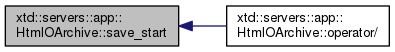
\includegraphics[width=350pt]{classxtd_1_1servers_1_1app_1_1HtmlOArchive_a8675544faff21c5a5acd0af123b48d6d_icgraph}
\end{center}
\end{figure}




\subsection{Friends And Related Function Documentation}
\index{xtd\+::servers\+::app\+::\+Html\+O\+Archive@{xtd\+::servers\+::app\+::\+Html\+O\+Archive}!boost\+::archive\+::basic\+\_\+xml\+\_\+oarchive$<$ Html\+O\+Archive $>$@{boost\+::archive\+::basic\+\_\+xml\+\_\+oarchive$<$ Html\+O\+Archive $>$}}
\index{boost\+::archive\+::basic\+\_\+xml\+\_\+oarchive$<$ Html\+O\+Archive $>$@{boost\+::archive\+::basic\+\_\+xml\+\_\+oarchive$<$ Html\+O\+Archive $>$}!xtd\+::servers\+::app\+::\+Html\+O\+Archive@{xtd\+::servers\+::app\+::\+Html\+O\+Archive}}
\subsubsection[{\texorpdfstring{boost\+::archive\+::basic\+\_\+xml\+\_\+oarchive$<$ Html\+O\+Archive $>$}{boost::archive::basic_xml_oarchive< HtmlOArchive >}}]{\setlength{\rightskip}{0pt plus 5cm}friend class boost\+::archive\+::basic\+\_\+xml\+\_\+oarchive$<$ {\bf Html\+O\+Archive} $>$\hspace{0.3cm}{\ttfamily [friend]}}\hypertarget{classxtd_1_1servers_1_1app_1_1HtmlOArchive_a350c2afaed5c679f01f1b4e36a6ad91f}{}\label{classxtd_1_1servers_1_1app_1_1HtmlOArchive_a350c2afaed5c679f01f1b4e36a6ad91f}


Definition at line 25 of file Html\+O\+Archive.\+hh.

\index{xtd\+::servers\+::app\+::\+Html\+O\+Archive@{xtd\+::servers\+::app\+::\+Html\+O\+Archive}!boost\+::archive\+::detail\+::interface\+\_\+oarchive$<$ Html\+O\+Archive $>$@{boost\+::archive\+::detail\+::interface\+\_\+oarchive$<$ Html\+O\+Archive $>$}}
\index{boost\+::archive\+::detail\+::interface\+\_\+oarchive$<$ Html\+O\+Archive $>$@{boost\+::archive\+::detail\+::interface\+\_\+oarchive$<$ Html\+O\+Archive $>$}!xtd\+::servers\+::app\+::\+Html\+O\+Archive@{xtd\+::servers\+::app\+::\+Html\+O\+Archive}}
\subsubsection[{\texorpdfstring{boost\+::archive\+::detail\+::interface\+\_\+oarchive$<$ Html\+O\+Archive $>$}{boost::archive::detail::interface_oarchive< HtmlOArchive >}}]{\setlength{\rightskip}{0pt plus 5cm}friend class boost\+::archive\+::detail\+::interface\+\_\+oarchive$<$ {\bf Html\+O\+Archive} $>$\hspace{0.3cm}{\ttfamily [friend]}}\hypertarget{classxtd_1_1servers_1_1app_1_1HtmlOArchive_a725f48824bde766dcd0e8049b4df3df0}{}\label{classxtd_1_1servers_1_1app_1_1HtmlOArchive_a725f48824bde766dcd0e8049b4df3df0}


Definition at line 24 of file Html\+O\+Archive.\+hh.

\index{xtd\+::servers\+::app\+::\+Html\+O\+Archive@{xtd\+::servers\+::app\+::\+Html\+O\+Archive}!boost\+::archive\+::save\+\_\+access@{boost\+::archive\+::save\+\_\+access}}
\index{boost\+::archive\+::save\+\_\+access@{boost\+::archive\+::save\+\_\+access}!xtd\+::servers\+::app\+::\+Html\+O\+Archive@{xtd\+::servers\+::app\+::\+Html\+O\+Archive}}
\subsubsection[{\texorpdfstring{boost\+::archive\+::save\+\_\+access}{boost::archive::save_access}}]{\setlength{\rightskip}{0pt plus 5cm}friend class boost\+::archive\+::save\+\_\+access\hspace{0.3cm}{\ttfamily [friend]}}\hypertarget{classxtd_1_1servers_1_1app_1_1HtmlOArchive_aaca003bb8a4fc59424e4025130da4edd}{}\label{classxtd_1_1servers_1_1app_1_1HtmlOArchive_aaca003bb8a4fc59424e4025130da4edd}


Definition at line 26 of file Html\+O\+Archive.\+hh.



\subsection{Member Data Documentation}
\index{xtd\+::servers\+::app\+::\+Html\+O\+Archive@{xtd\+::servers\+::app\+::\+Html\+O\+Archive}!m\+\_\+info@{m\+\_\+info}}
\index{m\+\_\+info@{m\+\_\+info}!xtd\+::servers\+::app\+::\+Html\+O\+Archive@{xtd\+::servers\+::app\+::\+Html\+O\+Archive}}
\subsubsection[{\texorpdfstring{m\+\_\+info}{m_info}}]{\setlength{\rightskip}{0pt plus 5cm}{\bf t\+\_\+info} xtd\+::servers\+::app\+::\+Html\+O\+Archive\+::m\+\_\+info}\hypertarget{classxtd_1_1servers_1_1app_1_1HtmlOArchive_a03bd854507f8457a3b5b575203108ff7}{}\label{classxtd_1_1servers_1_1app_1_1HtmlOArchive_a03bd854507f8457a3b5b575203108ff7}


Definition at line 182 of file Html\+O\+Archive.\+hh.

\index{xtd\+::servers\+::app\+::\+Html\+O\+Archive@{xtd\+::servers\+::app\+::\+Html\+O\+Archive}!m\+\_\+objects@{m\+\_\+objects}}
\index{m\+\_\+objects@{m\+\_\+objects}!xtd\+::servers\+::app\+::\+Html\+O\+Archive@{xtd\+::servers\+::app\+::\+Html\+O\+Archive}}
\subsubsection[{\texorpdfstring{m\+\_\+objects}{m_objects}}]{\setlength{\rightskip}{0pt plus 5cm}{\bf t\+\_\+objects} xtd\+::servers\+::app\+::\+Html\+O\+Archive\+::m\+\_\+objects}\hypertarget{classxtd_1_1servers_1_1app_1_1HtmlOArchive_a69e333ff9b2b0743e14976cfa4afd6d2}{}\label{classxtd_1_1servers_1_1app_1_1HtmlOArchive_a69e333ff9b2b0743e14976cfa4afd6d2}


Definition at line 183 of file Html\+O\+Archive.\+hh.



The documentation for this class was generated from the following files\+:\begin{DoxyCompactItemize}
\item 
/home/psyco/dev/xtdcpp/servers/src/app/\hyperlink{HtmlOArchive_8hh}{Html\+O\+Archive.\+hh}\item 
/home/psyco/dev/xtdcpp/servers/src/app/\hyperlink{HtmlOArchive_8cc}{Html\+O\+Archive.\+cc}\end{DoxyCompactItemize}

\hypertarget{classxtd_1_1servers_1_1app_1_1HttpServer}{\section{xtd\-:\-:servers\-:\-:app\-:\-:Http\-Server Class Reference}
\label{classxtd_1_1servers_1_1app_1_1HttpServer}\index{xtd\-::servers\-::app\-::\-Http\-Server@{xtd\-::servers\-::app\-::\-Http\-Server}}
}


{\ttfamily \#include $<$Http\-Server.\-hh$>$}



Inheritance diagram for xtd\-:\-:servers\-:\-:app\-:\-:Http\-Server\-:
\nopagebreak
\begin{figure}[H]
\begin{center}
\leavevmode
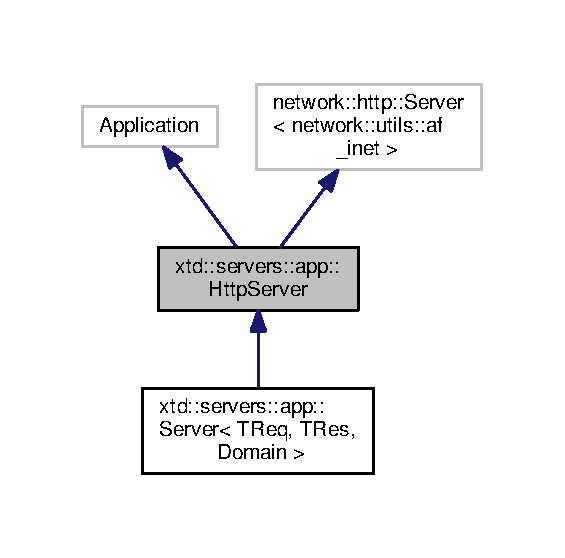
\includegraphics[width=271pt]{classxtd_1_1servers_1_1app_1_1HttpServer__inherit__graph}
\end{center}
\end{figure}


Collaboration diagram for xtd\-:\-:servers\-:\-:app\-:\-:Http\-Server\-:
\nopagebreak
\begin{figure}[H]
\begin{center}
\leavevmode
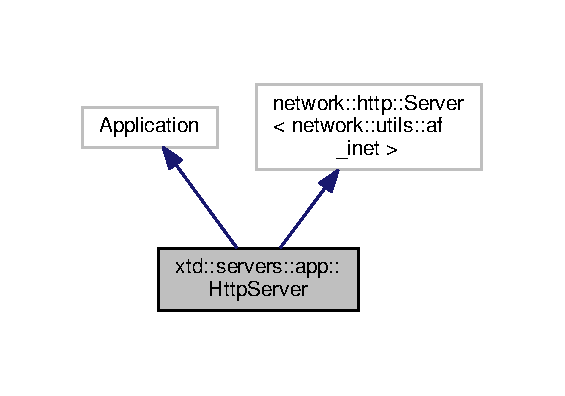
\includegraphics[width=271pt]{classxtd_1_1servers_1_1app_1_1HttpServer__coll__graph}
\end{center}
\end{figure}
\subsection*{Public Member Functions}
\begin{DoxyCompactItemize}
\item 
\hyperlink{classxtd_1_1servers_1_1app_1_1HttpServer_a3ebbe8af998a3e3738e41a72375ffea9}{Http\-Server} (bool p\-\_\-is\-Debug=false)
\item 
virtual \hyperlink{classxtd_1_1servers_1_1app_1_1HttpServer_a1082944f193865fc303c2d4a5569eaf9}{$\sim$\-Http\-Server} (void)
\end{DoxyCompactItemize}
\subsection*{Static Public Attributes}
\begin{DoxyCompactItemize}
\item 
static const uint32\-\_\-t \hyperlink{classxtd_1_1servers_1_1app_1_1HttpServer_a9ca36e61f5c201a51a68b3919e0badb7}{mcs\-\_\-default\-Probe\-Delay} = 30
\item 
static const uint32\-\_\-t \hyperlink{classxtd_1_1servers_1_1app_1_1HttpServer_abdc02697ffc7fa9f8f88252101b5d1b9}{mcs\-\_\-default\-Timeout\-Ms} = 5000
\item 
static const uint32\-\_\-t \hyperlink{classxtd_1_1servers_1_1app_1_1HttpServer_ad21741083478d35b92ba0b1da7499950}{mcs\-\_\-default\-Threshold\-Ms} = 0
\item 
static const char \hyperlink{classxtd_1_1servers_1_1app_1_1HttpServer_a38433b4c2d0bba9f0bae81266b42bac1}{mcs\-\_\-default\-Listen\-Interface} \mbox{[}$\,$\mbox{]} = \char`\"{}0.\-0.\-0.\-0\char`\"{}
\end{DoxyCompactItemize}
\subsection*{Protected Types}
\begin{DoxyCompactItemize}
\item 
typedef \hyperlink{classxtd_1_1servers_1_1app_1_1HttpServer}{Http\-Server} \hyperlink{classxtd_1_1servers_1_1app_1_1HttpServer_ad879d72fb0151a3c383ccbe75bb642cc}{http\-\_\-app}
\item 
typedef network\-::http\-::\-Server\\*
$<$ network\-::utils\-::af\-\_\-inet $>$ \hyperlink{classxtd_1_1servers_1_1app_1_1HttpServer_ac5263de622bb17c3ec921a00266ea053}{http\-\_\-net}
\item 
typedef boost\-::shared\-\_\-ptr\\*
$<$ \hyperlink{classxtd_1_1servers_1_1param_1_1Handler}{servers\-::param\-::\-Handler} $>$ \hyperlink{classxtd_1_1servers_1_1app_1_1HttpServer_a9704ed4f011ec3a7424da2f2229477e1}{t\-\_\-param\-\_\-handler}
\item 
typedef \\*
counters\-::\-Counter\-Manager\-::t\-\_\-sptr \hyperlink{classxtd_1_1servers_1_1app_1_1HttpServer_ace89439f838ede46ec55a6ec7cc27888}{t\-\_\-prober}
\item 
typedef boost\-::shared\-\_\-ptr$<$ \hyperlink{classxtd_1_1servers_1_1app_1_1Action}{Action} $>$ \hyperlink{classxtd_1_1servers_1_1app_1_1HttpServer_a1353c6e9098dd5f8a74d978a7049ad27}{t\-\_\-action}
\item 
typedef map$<$ string, \hyperlink{classxtd_1_1servers_1_1app_1_1HttpServer_a1353c6e9098dd5f8a74d978a7049ad27}{t\-\_\-action} $>$ \hyperlink{classxtd_1_1servers_1_1app_1_1HttpServer_ac61c9a29bf64b94cb8ca4c766f8309c3}{t\-\_\-actions}
\item 
typedef boost\-::shared\-\_\-ptr\\*
$<$ counters\-::\-Base $>$ \hyperlink{classxtd_1_1servers_1_1app_1_1HttpServer_aaef467afe1f5191f38758088615c09c0}{t\-\_\-counter}
\end{DoxyCompactItemize}
\subsection*{Protected Member Functions}
\begin{DoxyCompactItemize}
\item 
virtual string \hyperlink{classxtd_1_1servers_1_1app_1_1HttpServer_a3c838a2599ff485454ca19790ae0529c}{get\-Common\-Conf\-Key} (void) const 
\item 
virtual string \hyperlink{classxtd_1_1servers_1_1app_1_1HttpServer_a2b8fdc59d125cae41a833da5daf16d97}{get\-Specific\-Conf\-Key} (void) const 
\item 
virtual string \hyperlink{classxtd_1_1servers_1_1app_1_1HttpServer_affc53261a7c36873c73a06013d6b1fe6}{get\-Snmp\-Path} (void) const 
\item 
virtual void \hyperlink{classxtd_1_1servers_1_1app_1_1HttpServer_a022eecad815296f1d27b19a4b6cca908}{handle\-T\-E\-R\-M} (void)
\item 
virtual int \hyperlink{classxtd_1_1servers_1_1app_1_1HttpServer_a2b52e7d39c3b1937a4802bf7c3d159f8}{process} (void)
\item 
virtual void \hyperlink{classxtd_1_1servers_1_1app_1_1HttpServer_a7fdba08e0fa4dc9bbec30a989ccf4049}{stop} (void)
\item 
virtual void \hyperlink{classxtd_1_1servers_1_1app_1_1HttpServer_a6fac87218bf8d69ef6baeb56819411f9}{start} (void)
\item 
virtual void \hyperlink{classxtd_1_1servers_1_1app_1_1HttpServer_af4baf6c6e7397177a20122e1f1101f9f}{parse\-Config} (void)
\item 
virtual void \hyperlink{classxtd_1_1servers_1_1app_1_1HttpServer_a2b65812ed2afa6629f115b76c4ab6e41}{parse\-Http\-Port} (void)
\item 
virtual void \hyperlink{classxtd_1_1servers_1_1app_1_1HttpServer_a381e3736b9c8fa89891da50b29ad8ae9}{check\-Options} (void)
\item 
virtual void \hyperlink{classxtd_1_1servers_1_1app_1_1HttpServer_a0924e53b6bc9de7563c33690d619ce9d}{initialize} (void)
\item 
virtual status \hyperlink{classxtd_1_1servers_1_1app_1_1HttpServer_a66c2a3b5bca8390d96b35daebfccabf3}{define\-Probes} (void)
\item 
void \hyperlink{classxtd_1_1servers_1_1app_1_1HttpServer_a6c6bb7c70218f171e327ed2197d0f6dc}{handle\-U\-S\-R2} (void)
\item 
void \hyperlink{classxtd_1_1servers_1_1app_1_1HttpServer_a4b2a904b65659aa4e5d67d1ad4a02603}{mode\-Probe\-Activation} (void)
\item 
void \hyperlink{classxtd_1_1servers_1_1app_1_1HttpServer_a9247cbc7930939b40df98a20167007c3}{set\-Last\-Admin\-Log} (const string \&p\-\_\-message)
\item 
void \hyperlink{classxtd_1_1servers_1_1app_1_1HttpServer_a981ab09b5f746a0cb7372816aede1115}{bind\-\_\-action} (const string \&p\-\_\-name, const string \&p\-\_\-description, h p\-\_\-action)
\item 
status \hyperlink{classxtd_1_1servers_1_1app_1_1HttpServer_a89a77d0dd8391a54b9560d2a32ab5ec6}{h\-\_\-run\-Action} (const string \&p\-\_\-name, h p\-\_\-action, const uint32\-\_\-t p\-\_\-request\-Id, const network\-::http\-::\-Request \&p\-\_\-req, network\-::http\-::\-Response \&p\-\_\-res)
\item 
status \hyperlink{classxtd_1_1servers_1_1app_1_1HttpServer_a0ff20a40a0e31dbb1e82be87be0e255f}{add\-Probe} (\hyperlink{classxtd_1_1servers_1_1app_1_1HttpServer_aaef467afe1f5191f38758088615c09c0}{t\-\_\-counter} p\-\_\-counter, const string \&p\-\_\-path)
\item 
{\footnotesize template$<$typename T\-Type $>$ }\\status \hyperlink{classxtd_1_1servers_1_1app_1_1HttpServer_a6126daf3a088048921d4e809231c3716}{add\-Probe} (const T\-Type \&p\-\_\-value, const string \&p\-\_\-path, const string \&p\-\_\-name)
\item 
{\footnotesize template$<$typename T $>$ }\\status \hyperlink{classxtd_1_1servers_1_1app_1_1HttpServer_ae1cffd988b56081fba6f124e9f0743fd}{read\-Conf} (const std\-::string \&p\-\_\-key, T \&p\-\_\-dst, const T \&p\-\_\-default)
\item 
{\footnotesize template$<$typename T $>$ }\\status \hyperlink{classxtd_1_1servers_1_1app_1_1HttpServer_abe54ee996274b1f6d4a89d29bba56ae8}{read\-Conf} (const std\-::string \&p\-\_\-key, T \&p\-\_\-dst)
\end{DoxyCompactItemize}
\subsection*{Protected Attributes}
\begin{DoxyCompactItemize}
\item 
Conf\-Parser\-::t\-\_\-sptr \hyperlink{classxtd_1_1servers_1_1app_1_1HttpServer_ada282c895467a8d2fcaee543560958dc}{m\-\_\-config}
\item 
string \hyperlink{classxtd_1_1servers_1_1app_1_1HttpServer_aa07526617267875dd907e29b99711ab6}{m\-\_\-config\-Path}
\item 
size\-\_\-t \hyperlink{classxtd_1_1servers_1_1app_1_1HttpServer_a2f0812d24ccfd55e943f3144c672b473}{m\-\_\-nb\-Thread}
\item 
size\-\_\-t \hyperlink{classxtd_1_1servers_1_1app_1_1HttpServer_adcaefcc003e9503dbe6ebea90bf70ef7}{m\-\_\-timeout\-Ms}
\item 
bool \hyperlink{classxtd_1_1servers_1_1app_1_1HttpServer_a3ae2e35fc931b303e244b01e277cb8dd}{m\-\_\-is\-Mode\-Probe}
\item 
bool \hyperlink{classxtd_1_1servers_1_1app_1_1HttpServer_ae8b1e546b8f464e0a18c6b737ed82df8}{m\-\_\-is\-Debug}
\item 
string \hyperlink{classxtd_1_1servers_1_1app_1_1HttpServer_a555ce1e115602fda522a5c0a675dace3}{m\-\_\-snmp\-Path}
\item 
uint32\-\_\-t \hyperlink{classxtd_1_1servers_1_1app_1_1HttpServer_a87fc30b2e7e6ab2aabc2c46c884d7f17}{m\-\_\-probe\-Delay}
\item 
\hyperlink{classxtd_1_1servers_1_1app_1_1HttpServer_ace89439f838ede46ec55a6ec7cc27888}{t\-\_\-prober} \hyperlink{classxtd_1_1servers_1_1app_1_1HttpServer_aa26ddc958ab07774e8ba45e89dc0011b}{m\-\_\-prober}
\item 
counters\-::\-Value32\-::t\-\_\-sptr \hyperlink{classxtd_1_1servers_1_1app_1_1HttpServer_a0758f122d486bc068d796d4ce550e99f}{m\-\_\-ram\-Counter}
\item 
counters\-::\-Avg\-Timed\-Value\-::t\-\_\-sptr \hyperlink{classxtd_1_1servers_1_1app_1_1HttpServer_afc57d4c9bc2f9a47440e3c54eb92b1fb}{m\-\_\-perf\-Counter}
\item 
uint32\-\_\-t \hyperlink{classxtd_1_1servers_1_1app_1_1HttpServer_ad7f8a9a0475e17154850c3d575bf6f05}{m\-\_\-threshold\-Ms}
\item 
string \hyperlink{classxtd_1_1servers_1_1app_1_1HttpServer_af1676247676379d0c12008bdcd5b7e17}{m\-\_\-http\-Host}
\item 
uint32\-\_\-t \hyperlink{classxtd_1_1servers_1_1app_1_1HttpServer_a75ed3bcfa895cad365f6bf0955efcf9e}{m\-\_\-http\-Port}
\item 
network\-::utils\-::\-Config \hyperlink{classxtd_1_1servers_1_1app_1_1HttpServer_ad5f2480d758b731b641e4858f556a3c3}{m\-\_\-http\-Config}
\item 
string \hyperlink{classxtd_1_1servers_1_1app_1_1HttpServer_abfb9586e84fa5149da3226eeea39980f}{m\-\_\-http\-Config\-Path}
\item 
\hyperlink{classxtd_1_1servers_1_1app_1_1HttpServer_a9704ed4f011ec3a7424da2f2229477e1}{t\-\_\-param\-\_\-handler} \hyperlink{classxtd_1_1servers_1_1app_1_1HttpServer_ac4f9a2c40867f4f2ba8d30ec9876e51e}{m\-\_\-params}
\item 
string \hyperlink{classxtd_1_1servers_1_1app_1_1HttpServer_ad12543f950574ac8a0d813cb4ceeff4c}{m\-\_\-admin\-Dir}
\item 
\hyperlink{classxtd_1_1servers_1_1app_1_1HttpServer_ac61c9a29bf64b94cb8ca4c766f8309c3}{t\-\_\-actions} \hyperlink{classxtd_1_1servers_1_1app_1_1HttpServer_afa5363da18a3aa9de651e53e409116e9}{m\-\_\-actions}
\end{DoxyCompactItemize}


\subsection{Detailed Description}


Definition at line 47 of file Http\-Server.\-hh.



\subsection{Member Typedef Documentation}
\hypertarget{classxtd_1_1servers_1_1app_1_1HttpServer_ad879d72fb0151a3c383ccbe75bb642cc}{\index{xtd\-::servers\-::app\-::\-Http\-Server@{xtd\-::servers\-::app\-::\-Http\-Server}!http\-\_\-app@{http\-\_\-app}}
\index{http\-\_\-app@{http\-\_\-app}!xtd::servers::app::HttpServer@{xtd\-::servers\-::app\-::\-Http\-Server}}
\subsubsection[{http\-\_\-app}]{\setlength{\rightskip}{0pt plus 5cm}typedef {\bf Http\-Server} {\bf xtd\-::servers\-::app\-::\-Http\-Server\-::http\-\_\-app}\hspace{0.3cm}{\ttfamily [protected]}}}\label{classxtd_1_1servers_1_1app_1_1HttpServer_ad879d72fb0151a3c383ccbe75bb642cc}


Definition at line 64 of file Http\-Server.\-hh.

\hypertarget{classxtd_1_1servers_1_1app_1_1HttpServer_ac5263de622bb17c3ec921a00266ea053}{\index{xtd\-::servers\-::app\-::\-Http\-Server@{xtd\-::servers\-::app\-::\-Http\-Server}!http\-\_\-net@{http\-\_\-net}}
\index{http\-\_\-net@{http\-\_\-net}!xtd::servers::app::HttpServer@{xtd\-::servers\-::app\-::\-Http\-Server}}
\subsubsection[{http\-\_\-net}]{\setlength{\rightskip}{0pt plus 5cm}typedef network\-::http\-::\-Server$<$network\-::utils\-::af\-\_\-inet$>$ {\bf xtd\-::servers\-::app\-::\-Http\-Server\-::http\-\_\-net}\hspace{0.3cm}{\ttfamily [protected]}}}\label{classxtd_1_1servers_1_1app_1_1HttpServer_ac5263de622bb17c3ec921a00266ea053}


Definition at line 65 of file Http\-Server.\-hh.

\hypertarget{classxtd_1_1servers_1_1app_1_1HttpServer_a1353c6e9098dd5f8a74d978a7049ad27}{\index{xtd\-::servers\-::app\-::\-Http\-Server@{xtd\-::servers\-::app\-::\-Http\-Server}!t\-\_\-action@{t\-\_\-action}}
\index{t\-\_\-action@{t\-\_\-action}!xtd::servers::app::HttpServer@{xtd\-::servers\-::app\-::\-Http\-Server}}
\subsubsection[{t\-\_\-action}]{\setlength{\rightskip}{0pt plus 5cm}typedef boost\-::shared\-\_\-ptr$<${\bf Action}$>$ {\bf xtd\-::servers\-::app\-::\-Http\-Server\-::t\-\_\-action}\hspace{0.3cm}{\ttfamily [protected]}}}\label{classxtd_1_1servers_1_1app_1_1HttpServer_a1353c6e9098dd5f8a74d978a7049ad27}


Definition at line 68 of file Http\-Server.\-hh.

\hypertarget{classxtd_1_1servers_1_1app_1_1HttpServer_ac61c9a29bf64b94cb8ca4c766f8309c3}{\index{xtd\-::servers\-::app\-::\-Http\-Server@{xtd\-::servers\-::app\-::\-Http\-Server}!t\-\_\-actions@{t\-\_\-actions}}
\index{t\-\_\-actions@{t\-\_\-actions}!xtd::servers::app::HttpServer@{xtd\-::servers\-::app\-::\-Http\-Server}}
\subsubsection[{t\-\_\-actions}]{\setlength{\rightskip}{0pt plus 5cm}typedef map$<$string, {\bf t\-\_\-action}$>$ {\bf xtd\-::servers\-::app\-::\-Http\-Server\-::t\-\_\-actions}\hspace{0.3cm}{\ttfamily [protected]}}}\label{classxtd_1_1servers_1_1app_1_1HttpServer_ac61c9a29bf64b94cb8ca4c766f8309c3}


Definition at line 69 of file Http\-Server.\-hh.

\hypertarget{classxtd_1_1servers_1_1app_1_1HttpServer_aaef467afe1f5191f38758088615c09c0}{\index{xtd\-::servers\-::app\-::\-Http\-Server@{xtd\-::servers\-::app\-::\-Http\-Server}!t\-\_\-counter@{t\-\_\-counter}}
\index{t\-\_\-counter@{t\-\_\-counter}!xtd::servers::app::HttpServer@{xtd\-::servers\-::app\-::\-Http\-Server}}
\subsubsection[{t\-\_\-counter}]{\setlength{\rightskip}{0pt plus 5cm}typedef boost\-::shared\-\_\-ptr$<$counters\-::\-Base$>$ {\bf xtd\-::servers\-::app\-::\-Http\-Server\-::t\-\_\-counter}\hspace{0.3cm}{\ttfamily [protected]}}}\label{classxtd_1_1servers_1_1app_1_1HttpServer_aaef467afe1f5191f38758088615c09c0}


Definition at line 70 of file Http\-Server.\-hh.

\hypertarget{classxtd_1_1servers_1_1app_1_1HttpServer_a9704ed4f011ec3a7424da2f2229477e1}{\index{xtd\-::servers\-::app\-::\-Http\-Server@{xtd\-::servers\-::app\-::\-Http\-Server}!t\-\_\-param\-\_\-handler@{t\-\_\-param\-\_\-handler}}
\index{t\-\_\-param\-\_\-handler@{t\-\_\-param\-\_\-handler}!xtd::servers::app::HttpServer@{xtd\-::servers\-::app\-::\-Http\-Server}}
\subsubsection[{t\-\_\-param\-\_\-handler}]{\setlength{\rightskip}{0pt plus 5cm}typedef boost\-::shared\-\_\-ptr$<${\bf servers\-::param\-::\-Handler}$>$ {\bf xtd\-::servers\-::app\-::\-Http\-Server\-::t\-\_\-param\-\_\-handler}\hspace{0.3cm}{\ttfamily [protected]}}}\label{classxtd_1_1servers_1_1app_1_1HttpServer_a9704ed4f011ec3a7424da2f2229477e1}


Definition at line 66 of file Http\-Server.\-hh.

\hypertarget{classxtd_1_1servers_1_1app_1_1HttpServer_ace89439f838ede46ec55a6ec7cc27888}{\index{xtd\-::servers\-::app\-::\-Http\-Server@{xtd\-::servers\-::app\-::\-Http\-Server}!t\-\_\-prober@{t\-\_\-prober}}
\index{t\-\_\-prober@{t\-\_\-prober}!xtd::servers::app::HttpServer@{xtd\-::servers\-::app\-::\-Http\-Server}}
\subsubsection[{t\-\_\-prober}]{\setlength{\rightskip}{0pt plus 5cm}typedef counters\-::\-Counter\-Manager\-::t\-\_\-sptr {\bf xtd\-::servers\-::app\-::\-Http\-Server\-::t\-\_\-prober}\hspace{0.3cm}{\ttfamily [protected]}}}\label{classxtd_1_1servers_1_1app_1_1HttpServer_ace89439f838ede46ec55a6ec7cc27888}


Definition at line 67 of file Http\-Server.\-hh.



\subsection{Constructor \& Destructor Documentation}
\hypertarget{classxtd_1_1servers_1_1app_1_1HttpServer_a3ebbe8af998a3e3738e41a72375ffea9}{\index{xtd\-::servers\-::app\-::\-Http\-Server@{xtd\-::servers\-::app\-::\-Http\-Server}!Http\-Server@{Http\-Server}}
\index{Http\-Server@{Http\-Server}!xtd::servers::app::HttpServer@{xtd\-::servers\-::app\-::\-Http\-Server}}
\subsubsection[{Http\-Server}]{\setlength{\rightskip}{0pt plus 5cm}xtd\-::servers\-::app\-::\-Http\-Server\-::\-Http\-Server (
\begin{DoxyParamCaption}
\item[{bool}]{p\-\_\-is\-Debug = {\ttfamily false}}
\end{DoxyParamCaption}
)}}\label{classxtd_1_1servers_1_1app_1_1HttpServer_a3ebbe8af998a3e3738e41a72375ffea9}


Definition at line 38 of file Http\-Server.\-cc.


\begin{DoxyCode}
38                                      :
39   Application(),
40   \hyperlink{classxtd_1_1servers_1_1app_1_1HttpServer_ac5263de622bb17c3ec921a00266ea053}{http\_net}(),
41   \hyperlink{classxtd_1_1servers_1_1app_1_1HttpServer_ada282c895467a8d2fcaee543560958dc}{m\_config}(0),
42   \hyperlink{classxtd_1_1servers_1_1app_1_1HttpServer_aa07526617267875dd907e29b99711ab6}{m\_configPath}(),
43   \hyperlink{classxtd_1_1servers_1_1app_1_1HttpServer_a2f0812d24ccfd55e943f3144c672b473}{m\_nbThread}(0),
44   \hyperlink{classxtd_1_1servers_1_1app_1_1HttpServer_adcaefcc003e9503dbe6ebea90bf70ef7}{m\_timeoutMs}(\hyperlink{classxtd_1_1servers_1_1app_1_1HttpServer_abdc02697ffc7fa9f8f88252101b5d1b9}{mcs\_defaultTimeoutMs}),
45   \hyperlink{classxtd_1_1servers_1_1app_1_1HttpServer_a3ae2e35fc931b303e244b01e277cb8dd}{m\_isModeProbe}(\textcolor{keyword}{false}),
46   \hyperlink{classxtd_1_1servers_1_1app_1_1HttpServer_ae8b1e546b8f464e0a18c6b737ed82df8}{m\_isDebug}(p\_isDebug),
47   \hyperlink{classxtd_1_1servers_1_1app_1_1HttpServer_a555ce1e115602fda522a5c0a675dace3}{m\_snmpPath}(\textcolor{stringliteral}{"/var/run/xtd/snmp/"}),
48   \hyperlink{classxtd_1_1servers_1_1app_1_1HttpServer_a87fc30b2e7e6ab2aabc2c46c884d7f17}{m\_probeDelay}(\hyperlink{classxtd_1_1servers_1_1app_1_1HttpServer_a9ca36e61f5c201a51a68b3919e0badb7}{mcs\_defaultProbeDelay}),
49   \hyperlink{classxtd_1_1servers_1_1app_1_1HttpServer_aa26ddc958ab07774e8ba45e89dc0011b}{m\_prober}(),
50   \hyperlink{classxtd_1_1servers_1_1app_1_1HttpServer_a0758f122d486bc068d796d4ce550e99f}{m\_ramCounter}(),
51   \hyperlink{classxtd_1_1servers_1_1app_1_1HttpServer_afc57d4c9bc2f9a47440e3c54eb92b1fb}{m\_perfCounter}(),
52   \hyperlink{classxtd_1_1servers_1_1app_1_1HttpServer_ad7f8a9a0475e17154850c3d575bf6f05}{m\_thresholdMs}(\hyperlink{classxtd_1_1servers_1_1app_1_1HttpServer_ad21741083478d35b92ba0b1da7499950}{mcs\_defaultThresholdMs}),
53   \hyperlink{classxtd_1_1servers_1_1app_1_1HttpServer_af1676247676379d0c12008bdcd5b7e17}{m\_httpHost}(\hyperlink{classxtd_1_1servers_1_1app_1_1HttpServer_a38433b4c2d0bba9f0bae81266b42bac1}{mcs\_defaultListenInterface}),
54   \hyperlink{classxtd_1_1servers_1_1app_1_1HttpServer_a75ed3bcfa895cad365f6bf0955efcf9e}{m\_httpPort}(0),
55   \hyperlink{classxtd_1_1servers_1_1app_1_1HttpServer_ad5f2480d758b731b641e4858f556a3c3}{m\_httpConfig}(),
56   \hyperlink{classxtd_1_1servers_1_1app_1_1HttpServer_abfb9586e84fa5149da3226eeea39980f}{m\_httpConfigPath}(\textcolor{stringliteral}{"/usr/lib/xtd/www"}),
57   \hyperlink{classxtd_1_1servers_1_1app_1_1HttpServer_ad12543f950574ac8a0d813cb4ceeff4c}{m\_adminDir}(\textcolor{stringliteral}{"/var/run/xtd/snmp/admin"}),
58   \hyperlink{classxtd_1_1servers_1_1app_1_1HttpServer_afa5363da18a3aa9de651e53e409116e9}{m\_actions}()
59 \{
60   addOption(\textcolor{charliteral}{'c'}, \textcolor{stringliteral}{"config-file"}, argument::mandatory, requirement::mandatory, \textcolor{stringliteral}{"use <file> as input config
       file"},                bindFile(\hyperlink{classxtd_1_1servers_1_1app_1_1HttpServer_aa07526617267875dd907e29b99711ab6}{m\_configPath}));
61   addOption(\textcolor{charliteral}{'w'}, \textcolor{stringliteral}{"http-port"},   argument::mandatory, requirement::optional,  \textcolor{stringliteral}{"use <port> as http server
       port"},                 bindNumber(\hyperlink{classxtd_1_1servers_1_1app_1_1HttpServer_a75ed3bcfa895cad365f6bf0955efcf9e}{m\_httpPort}));
62   addOption(\textcolor{charliteral}{'n'}, \textcolor{stringliteral}{"nb-thread"},   argument::mandatory, requirement::optional,  \textcolor{stringliteral}{"allocates <nbr> threads for
       incomming requests"}, bindNumber(\hyperlink{classxtd_1_1servers_1_1app_1_1HttpServer_a2f0812d24ccfd55e943f3144c672b473}{m\_nbThread}));
63   addOption(\textcolor{charliteral}{'t'}, \textcolor{stringliteral}{"timeout"},     argument::mandatory, requirement::optional,  \textcolor{stringliteral}{"server timeout in ms"},       
                          bindNumber(\hyperlink{classxtd_1_1servers_1_1app_1_1HttpServer_adcaefcc003e9503dbe6ebea90bf70ef7}{m\_timeoutMs}));
64 
65   \hyperlink{classxtd_1_1servers_1_1app_1_1HttpServer_ad5f2480d758b731b641e4858f556a3c3}{m\_httpConfig}.setReuseAddr(\textcolor{keyword}{true});
66   addSignalHandler(SIGUSR2, boost::bind(&\hyperlink{classxtd_1_1servers_1_1app_1_1HttpServer_a6c6bb7c70218f171e327ed2197d0f6dc}{HttpServer::handleUSR2}, \textcolor{keyword}{this}));
67   addSignalHandler(SIGTERM, boost::bind(&\hyperlink{classxtd_1_1servers_1_1app_1_1HttpServer_a022eecad815296f1d27b19a4b6cca908}{HttpServer::handleTERM}, \textcolor{keyword}{this}));
68 \}
\end{DoxyCode}


Here is the call graph for this function\-:
\nopagebreak
\begin{figure}[H]
\begin{center}
\leavevmode
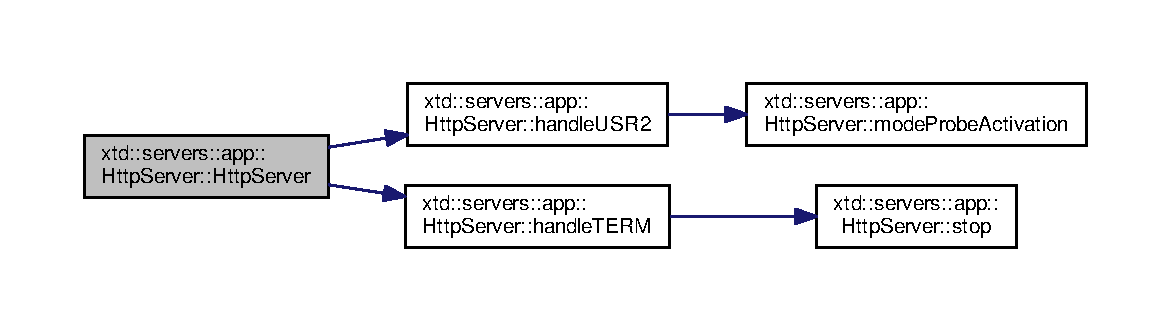
\includegraphics[width=350pt]{classxtd_1_1servers_1_1app_1_1HttpServer_a3ebbe8af998a3e3738e41a72375ffea9_cgraph}
\end{center}
\end{figure}


\hypertarget{classxtd_1_1servers_1_1app_1_1HttpServer_a1082944f193865fc303c2d4a5569eaf9}{\index{xtd\-::servers\-::app\-::\-Http\-Server@{xtd\-::servers\-::app\-::\-Http\-Server}!$\sim$\-Http\-Server@{$\sim$\-Http\-Server}}
\index{$\sim$\-Http\-Server@{$\sim$\-Http\-Server}!xtd::servers::app::HttpServer@{xtd\-::servers\-::app\-::\-Http\-Server}}
\subsubsection[{$\sim$\-Http\-Server}]{\setlength{\rightskip}{0pt plus 5cm}xtd\-::servers\-::app\-::\-Http\-Server\-::$\sim$\-Http\-Server (
\begin{DoxyParamCaption}
\item[{void}]{}
\end{DoxyParamCaption}
)\hspace{0.3cm}{\ttfamily [virtual]}}}\label{classxtd_1_1servers_1_1app_1_1HttpServer_a1082944f193865fc303c2d4a5569eaf9}


Definition at line 70 of file Http\-Server.\-cc.


\begin{DoxyCode}
71 \{
72 \}
\end{DoxyCode}


\subsection{Member Function Documentation}
\hypertarget{classxtd_1_1servers_1_1app_1_1HttpServer_a0ff20a40a0e31dbb1e82be87be0e255f}{\index{xtd\-::servers\-::app\-::\-Http\-Server@{xtd\-::servers\-::app\-::\-Http\-Server}!add\-Probe@{add\-Probe}}
\index{add\-Probe@{add\-Probe}!xtd::servers::app::HttpServer@{xtd\-::servers\-::app\-::\-Http\-Server}}
\subsubsection[{add\-Probe}]{\setlength{\rightskip}{0pt plus 5cm}status xtd\-::servers\-::app\-::\-Http\-Server\-::add\-Probe (
\begin{DoxyParamCaption}
\item[{{\bf t\-\_\-counter}}]{p\-\_\-counter, }
\item[{const string \&}]{p\-\_\-path}
\end{DoxyParamCaption}
)\hspace{0.3cm}{\ttfamily [protected]}}}\label{classxtd_1_1servers_1_1app_1_1HttpServer_a0ff20a40a0e31dbb1e82be87be0e255f}


Definition at line 206 of file Http\-Server.\-cc.


\begin{DoxyCode}
207 \{
208   \textcolor{keywordflow}{if} (status::ok != \hyperlink{classxtd_1_1servers_1_1app_1_1HttpServer_aa26ddc958ab07774e8ba45e89dc0011b}{m\_prober}->add(p\_counter, p\_path))
209     \textcolor{keywordflow}{return} status::error;
210   \textcolor{keywordflow}{return} status::ok;
211 \}
\end{DoxyCode}


Here is the caller graph for this function\-:
\nopagebreak
\begin{figure}[H]
\begin{center}
\leavevmode
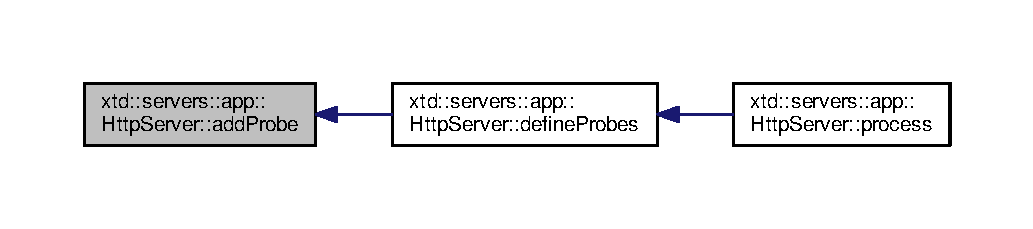
\includegraphics[width=350pt]{classxtd_1_1servers_1_1app_1_1HttpServer_a0ff20a40a0e31dbb1e82be87be0e255f_icgraph}
\end{center}
\end{figure}


\hypertarget{classxtd_1_1servers_1_1app_1_1HttpServer_a6126daf3a088048921d4e809231c3716}{\index{xtd\-::servers\-::app\-::\-Http\-Server@{xtd\-::servers\-::app\-::\-Http\-Server}!add\-Probe@{add\-Probe}}
\index{add\-Probe@{add\-Probe}!xtd::servers::app::HttpServer@{xtd\-::servers\-::app\-::\-Http\-Server}}
\subsubsection[{add\-Probe}]{\setlength{\rightskip}{0pt plus 5cm}template$<$typename T\-Type $>$ status xtd\-::servers\-::app\-::\-Http\-Server\-::add\-Probe (
\begin{DoxyParamCaption}
\item[{const T\-Type \&}]{p\-\_\-value, }
\item[{const string \&}]{p\-\_\-path, }
\item[{const string \&}]{p\-\_\-name}
\end{DoxyParamCaption}
)\hspace{0.3cm}{\ttfamily [protected]}}}\label{classxtd_1_1servers_1_1app_1_1HttpServer_a6126daf3a088048921d4e809231c3716}
\hypertarget{classxtd_1_1servers_1_1app_1_1HttpServer_a981ab09b5f746a0cb7372816aede1115}{\index{xtd\-::servers\-::app\-::\-Http\-Server@{xtd\-::servers\-::app\-::\-Http\-Server}!bind\-\_\-action@{bind\-\_\-action}}
\index{bind\-\_\-action@{bind\-\_\-action}!xtd::servers::app::HttpServer@{xtd\-::servers\-::app\-::\-Http\-Server}}
\subsubsection[{bind\-\_\-action}]{\setlength{\rightskip}{0pt plus 5cm}void xtd\-::servers\-::app\-::\-Http\-Server\-::bind\-\_\-action (
\begin{DoxyParamCaption}
\item[{const string \&}]{p\-\_\-name, }
\item[{const string \&}]{p\-\_\-description, }
\item[{h}]{p\-\_\-action}
\end{DoxyParamCaption}
)\hspace{0.3cm}{\ttfamily [protected]}}}\label{classxtd_1_1servers_1_1app_1_1HttpServer_a981ab09b5f746a0cb7372816aede1115}


Definition at line 318 of file Http\-Server.\-cc.


\begin{DoxyCode}
321 \{
322   \hyperlink{classxtd_1_1servers_1_1app_1_1HttpServer_a1353c6e9098dd5f8a74d978a7049ad27}{t\_action} l\_action(\textcolor{keyword}{new} Action(p\_name, p\_description));
323 
324   \hyperlink{classxtd_1_1servers_1_1app_1_1HttpServer_afa5363da18a3aa9de651e53e409116e9}{m\_actions}.insert(std::pair<string, t\_action>(p\_name, l\_action));
325   bind(\textcolor{stringliteral}{"/action/"} + p\_name, h(&\hyperlink{classxtd_1_1servers_1_1app_1_1HttpServer_a89a77d0dd8391a54b9560d2a32ab5ec6}{HttpServer::h\_runAction}, \textcolor{keyword}{this}, p\_name, p\_action));
326 \}
\end{DoxyCode}


Here is the call graph for this function\-:
\nopagebreak
\begin{figure}[H]
\begin{center}
\leavevmode
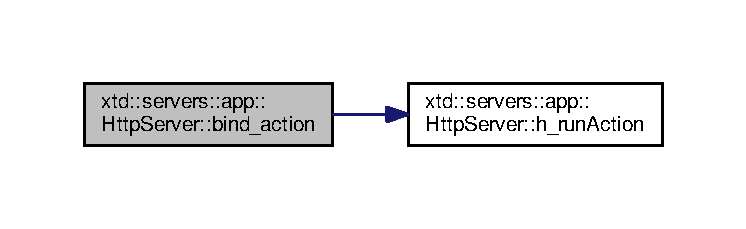
\includegraphics[width=350pt]{classxtd_1_1servers_1_1app_1_1HttpServer_a981ab09b5f746a0cb7372816aede1115_cgraph}
\end{center}
\end{figure}


\hypertarget{classxtd_1_1servers_1_1app_1_1HttpServer_a381e3736b9c8fa89891da50b29ad8ae9}{\index{xtd\-::servers\-::app\-::\-Http\-Server@{xtd\-::servers\-::app\-::\-Http\-Server}!check\-Options@{check\-Options}}
\index{check\-Options@{check\-Options}!xtd::servers::app::HttpServer@{xtd\-::servers\-::app\-::\-Http\-Server}}
\subsubsection[{check\-Options}]{\setlength{\rightskip}{0pt plus 5cm}void xtd\-::servers\-::app\-::\-Http\-Server\-::check\-Options (
\begin{DoxyParamCaption}
\item[{void}]{}
\end{DoxyParamCaption}
)\hspace{0.3cm}{\ttfamily [protected]}, {\ttfamily [virtual]}}}\label{classxtd_1_1servers_1_1app_1_1HttpServer_a381e3736b9c8fa89891da50b29ad8ae9}


Reimplemented in \hyperlink{classxtd_1_1servers_1_1app_1_1Server_a6f5fff5c5058dc43aea7b27a046c985b}{xtd\-::servers\-::app\-::\-Server$<$ T\-Req, T\-Res, Domain $>$}.



Definition at line 193 of file Http\-Server.\-cc.


\begin{DoxyCode}
194 \{
195   \textcolor{keywordflow}{if} ((\hyperlink{classxtd_1_1servers_1_1app_1_1HttpServer_a75ed3bcfa895cad365f6bf0955efcf9e}{m\_httpPort} == 0) || (\hyperlink{classxtd_1_1servers_1_1app_1_1HttpServer_a75ed3bcfa895cad365f6bf0955efcf9e}{m\_httpPort} > 65535))
196     error\_nohelp(1, \textcolor{stringliteral}{"invalid --http-port '%d', must have 0 < port < 65536"}, 
      \hyperlink{classxtd_1_1servers_1_1app_1_1HttpServer_a75ed3bcfa895cad365f6bf0955efcf9e}{m\_httpPort});
197 
198   \textcolor{keywordflow}{if} ((\hyperlink{classxtd_1_1servers_1_1app_1_1HttpServer_a2f0812d24ccfd55e943f3144c672b473}{m\_nbThread} == 0) || (\hyperlink{classxtd_1_1servers_1_1app_1_1HttpServer_a2f0812d24ccfd55e943f3144c672b473}{m\_nbThread} > 1000))
199     error\_nohelp(1, \textcolor{stringliteral}{"invalid --nb-thread='%d', must have 0 < nbr <= 1000"}, 
      \hyperlink{classxtd_1_1servers_1_1app_1_1HttpServer_a2f0812d24ccfd55e943f3144c672b473}{m\_nbThread});
200 
201   \textcolor{keywordflow}{if} (\hyperlink{classxtd_1_1servers_1_1app_1_1HttpServer_adcaefcc003e9503dbe6ebea90bf70ef7}{m\_timeoutMs} < 100)
202     error\_nohelp(1, \textcolor{stringliteral}{"invalid --timeout='%d', must have 100 <= nbr"}, \hyperlink{classxtd_1_1servers_1_1app_1_1HttpServer_a2f0812d24ccfd55e943f3144c672b473}{m\_nbThread});
203 \}
\end{DoxyCode}
\hypertarget{classxtd_1_1servers_1_1app_1_1HttpServer_a66c2a3b5bca8390d96b35daebfccabf3}{\index{xtd\-::servers\-::app\-::\-Http\-Server@{xtd\-::servers\-::app\-::\-Http\-Server}!define\-Probes@{define\-Probes}}
\index{define\-Probes@{define\-Probes}!xtd::servers::app::HttpServer@{xtd\-::servers\-::app\-::\-Http\-Server}}
\subsubsection[{define\-Probes}]{\setlength{\rightskip}{0pt plus 5cm}status xtd\-::servers\-::app\-::\-Http\-Server\-::define\-Probes (
\begin{DoxyParamCaption}
\item[{void}]{}
\end{DoxyParamCaption}
)\hspace{0.3cm}{\ttfamily [protected]}, {\ttfamily [virtual]}}}\label{classxtd_1_1servers_1_1app_1_1HttpServer_a66c2a3b5bca8390d96b35daebfccabf3}


Reimplemented in \hyperlink{classxtd_1_1servers_1_1app_1_1Server_afbe76a86e66e635907229d37b1267037}{xtd\-::servers\-::app\-::\-Server$<$ T\-Req, T\-Res, Domain $>$}.



Definition at line 215 of file Http\-Server.\-cc.


\begin{DoxyCode}
216 \{
217   \textcolor{keywordtype}{string} l\_dir = \hyperlink{classxtd_1_1servers_1_1app_1_1HttpServer_ae8b1e546b8f464e0a18c6b737ed82df8}{m\_isDebug} ? \textcolor{stringliteral}{"server\_http"} : \textcolor{stringliteral}{"server"};
218 
219   \textcolor{keywordflow}{if} ((status::ok != \hyperlink{classxtd_1_1servers_1_1app_1_1HttpServer_a0ff20a40a0e31dbb1e82be87be0e255f}{addProbe}(\hyperlink{classxtd_1_1servers_1_1app_1_1HttpServer_a0758f122d486bc068d796d4ce550e99f}{m\_ramCounter},                    \textcolor{stringliteral}{""}                      
          )) ||
220       (status::ok != \hyperlink{classxtd_1_1servers_1_1app_1_1HttpServer_a0ff20a40a0e31dbb1e82be87be0e255f}{addProbe}(\hyperlink{classxtd_1_1servers_1_1app_1_1HttpServer_afc57d4c9bc2f9a47440e3c54eb92b1fb}{http\_app::m\_perfCounter},         l\_dir        
                     )) ||
221       (status::ok != \hyperlink{classxtd_1_1servers_1_1app_1_1HttpServer_a0ff20a40a0e31dbb1e82be87be0e255f}{addProbe}(http\_net::getReceiveTotal(),     l\_dir,        \textcolor{stringliteral}{"qry.total"}   )) ||
222       (status::ok != \hyperlink{classxtd_1_1servers_1_1app_1_1HttpServer_a0ff20a40a0e31dbb1e82be87be0e255f}{addProbe}(http\_net::getReceiveError(),     l\_dir,        \textcolor{stringliteral}{"qry.error"}   )) ||
223       (status::ok != \hyperlink{classxtd_1_1servers_1_1app_1_1HttpServer_a0ff20a40a0e31dbb1e82be87be0e255f}{addProbe}(http\_net::getReceiveTimeout(),   l\_dir,        \textcolor{stringliteral}{"qry.timeout"} )) ||
224       (status::ok != \hyperlink{classxtd_1_1servers_1_1app_1_1HttpServer_a0ff20a40a0e31dbb1e82be87be0e255f}{addProbe}(http\_net::getReceiveSuccess(),   l\_dir,        \textcolor{stringliteral}{"qry.success"} )) ||
225       (status::ok != \hyperlink{classxtd_1_1servers_1_1app_1_1HttpServer_a0ff20a40a0e31dbb1e82be87be0e255f}{addProbe}(http\_net::getReceivedLastTime(), l\_dir,        \textcolor{stringliteral}{"qry.lasttime"})) ||
226       (status::ok != \hyperlink{classxtd_1_1servers_1_1app_1_1HttpServer_a0ff20a40a0e31dbb1e82be87be0e255f}{addProbe}(http\_net::getSendTotal(),        l\_dir,        \textcolor{stringliteral}{"rsp.total"}   )) ||
227       (status::ok != \hyperlink{classxtd_1_1servers_1_1app_1_1HttpServer_a0ff20a40a0e31dbb1e82be87be0e255f}{addProbe}(http\_net::getSendSuccess(),      l\_dir,        \textcolor{stringliteral}{"rsp.success"} )) ||
228       (status::ok != \hyperlink{classxtd_1_1servers_1_1app_1_1HttpServer_a0ff20a40a0e31dbb1e82be87be0e255f}{addProbe}(http\_net::getSendTimeout(),      l\_dir,        \textcolor{stringliteral}{"rsp.timeout"} )) ||
229       (status::ok != \hyperlink{classxtd_1_1servers_1_1app_1_1HttpServer_a0ff20a40a0e31dbb1e82be87be0e255f}{addProbe}(http\_net::getSendError(),        l\_dir,        \textcolor{stringliteral}{"rsp.error"}   )) ||
230       (status::ok != \hyperlink{classxtd_1_1servers_1_1app_1_1HttpServer_a0ff20a40a0e31dbb1e82be87be0e255f}{addProbe}(http\_net::getCnxTotal(),         l\_dir,        \textcolor{stringliteral}{"cnx.total"}   )) ||
231       (status::ok != \hyperlink{classxtd_1_1servers_1_1app_1_1HttpServer_a0ff20a40a0e31dbb1e82be87be0e255f}{addProbe}(http\_net::getCnxAccepted(),      l\_dir,        \textcolor{stringliteral}{"cnx.accepted"})) ||
232       (status::ok != \hyperlink{classxtd_1_1servers_1_1app_1_1HttpServer_a0ff20a40a0e31dbb1e82be87be0e255f}{addProbe}(http\_net::getCnxRejected(),      l\_dir,        \textcolor{stringliteral}{"cnx.rejected"})) ||
233       (status::ok != \hyperlink{classxtd_1_1servers_1_1app_1_1HttpServer_a0ff20a40a0e31dbb1e82be87be0e255f}{addProbe}(http\_net::getNbCurrentThread(),  l\_dir,        \textcolor{stringliteral}{"threads"}     )))
234     \textcolor{keywordflow}{return} status::error;
235   \textcolor{keywordflow}{return} status::ok;
236 \}
\end{DoxyCode}


Here is the call graph for this function\-:
\nopagebreak
\begin{figure}[H]
\begin{center}
\leavevmode
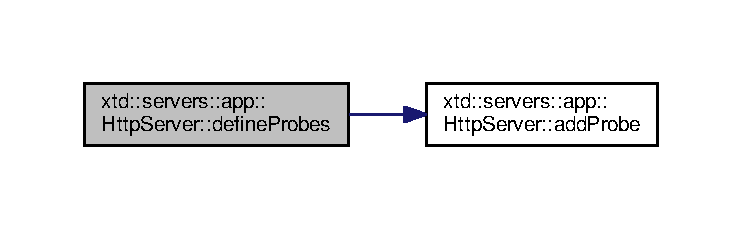
\includegraphics[width=350pt]{classxtd_1_1servers_1_1app_1_1HttpServer_a66c2a3b5bca8390d96b35daebfccabf3_cgraph}
\end{center}
\end{figure}




Here is the caller graph for this function\-:
\nopagebreak
\begin{figure}[H]
\begin{center}
\leavevmode
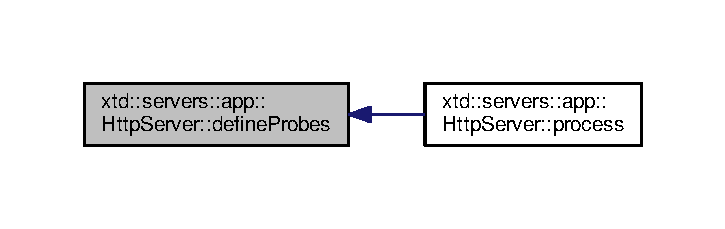
\includegraphics[width=348pt]{classxtd_1_1servers_1_1app_1_1HttpServer_a66c2a3b5bca8390d96b35daebfccabf3_icgraph}
\end{center}
\end{figure}


\hypertarget{classxtd_1_1servers_1_1app_1_1HttpServer_a3c838a2599ff485454ca19790ae0529c}{\index{xtd\-::servers\-::app\-::\-Http\-Server@{xtd\-::servers\-::app\-::\-Http\-Server}!get\-Common\-Conf\-Key@{get\-Common\-Conf\-Key}}
\index{get\-Common\-Conf\-Key@{get\-Common\-Conf\-Key}!xtd::servers::app::HttpServer@{xtd\-::servers\-::app\-::\-Http\-Server}}
\subsubsection[{get\-Common\-Conf\-Key}]{\setlength{\rightskip}{0pt plus 5cm}string xtd\-::servers\-::app\-::\-Http\-Server\-::get\-Common\-Conf\-Key (
\begin{DoxyParamCaption}
\item[{void}]{}
\end{DoxyParamCaption}
) const\hspace{0.3cm}{\ttfamily [protected]}, {\ttfamily [virtual]}}}\label{classxtd_1_1servers_1_1app_1_1HttpServer_a3c838a2599ff485454ca19790ae0529c}


Definition at line 423 of file Http\-Server.\-cc.


\begin{DoxyCode}
424 \{
425   \textcolor{keywordflow}{return} m\_binName;
426 \}
\end{DoxyCode}


Here is the caller graph for this function\-:
\nopagebreak
\begin{figure}[H]
\begin{center}
\leavevmode
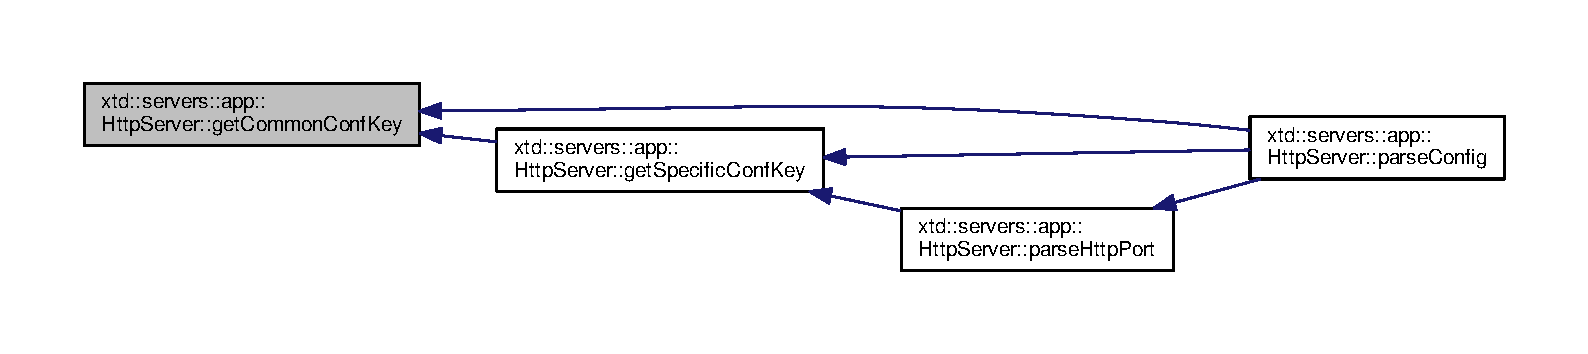
\includegraphics[width=350pt]{classxtd_1_1servers_1_1app_1_1HttpServer_a3c838a2599ff485454ca19790ae0529c_icgraph}
\end{center}
\end{figure}


\hypertarget{classxtd_1_1servers_1_1app_1_1HttpServer_affc53261a7c36873c73a06013d6b1fe6}{\index{xtd\-::servers\-::app\-::\-Http\-Server@{xtd\-::servers\-::app\-::\-Http\-Server}!get\-Snmp\-Path@{get\-Snmp\-Path}}
\index{get\-Snmp\-Path@{get\-Snmp\-Path}!xtd::servers::app::HttpServer@{xtd\-::servers\-::app\-::\-Http\-Server}}
\subsubsection[{get\-Snmp\-Path}]{\setlength{\rightskip}{0pt plus 5cm}string xtd\-::servers\-::app\-::\-Http\-Server\-::get\-Snmp\-Path (
\begin{DoxyParamCaption}
\item[{void}]{}
\end{DoxyParamCaption}
) const\hspace{0.3cm}{\ttfamily [protected]}, {\ttfamily [virtual]}}}\label{classxtd_1_1servers_1_1app_1_1HttpServer_affc53261a7c36873c73a06013d6b1fe6}


Definition at line 435 of file Http\-Server.\-cc.


\begin{DoxyCode}
436 \{
437   \textcolor{keywordflow}{return} \hyperlink{classxtd_1_1servers_1_1app_1_1HttpServer_a555ce1e115602fda522a5c0a675dace3}{m\_snmpPath};
438 \}
\end{DoxyCode}


Here is the caller graph for this function\-:
\nopagebreak
\begin{figure}[H]
\begin{center}
\leavevmode
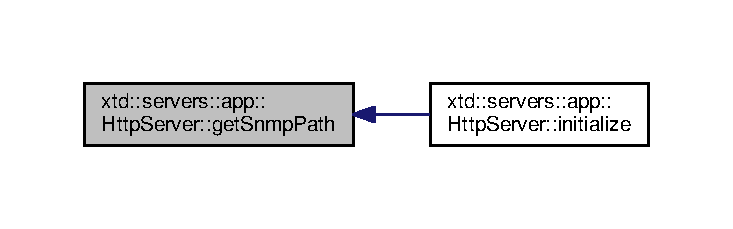
\includegraphics[width=350pt]{classxtd_1_1servers_1_1app_1_1HttpServer_affc53261a7c36873c73a06013d6b1fe6_icgraph}
\end{center}
\end{figure}


\hypertarget{classxtd_1_1servers_1_1app_1_1HttpServer_a2b8fdc59d125cae41a833da5daf16d97}{\index{xtd\-::servers\-::app\-::\-Http\-Server@{xtd\-::servers\-::app\-::\-Http\-Server}!get\-Specific\-Conf\-Key@{get\-Specific\-Conf\-Key}}
\index{get\-Specific\-Conf\-Key@{get\-Specific\-Conf\-Key}!xtd::servers::app::HttpServer@{xtd\-::servers\-::app\-::\-Http\-Server}}
\subsubsection[{get\-Specific\-Conf\-Key}]{\setlength{\rightskip}{0pt plus 5cm}string xtd\-::servers\-::app\-::\-Http\-Server\-::get\-Specific\-Conf\-Key (
\begin{DoxyParamCaption}
\item[{void}]{}
\end{DoxyParamCaption}
) const\hspace{0.3cm}{\ttfamily [protected]}, {\ttfamily [virtual]}}}\label{classxtd_1_1servers_1_1app_1_1HttpServer_a2b8fdc59d125cae41a833da5daf16d97}


Definition at line 429 of file Http\-Server.\-cc.


\begin{DoxyCode}
430 \{
431   \textcolor{keywordflow}{return} \hyperlink{classxtd_1_1servers_1_1app_1_1HttpServer_a3c838a2599ff485454ca19790ae0529c}{getCommonConfKey}();
432 \}
\end{DoxyCode}


Here is the call graph for this function\-:
\nopagebreak
\begin{figure}[H]
\begin{center}
\leavevmode
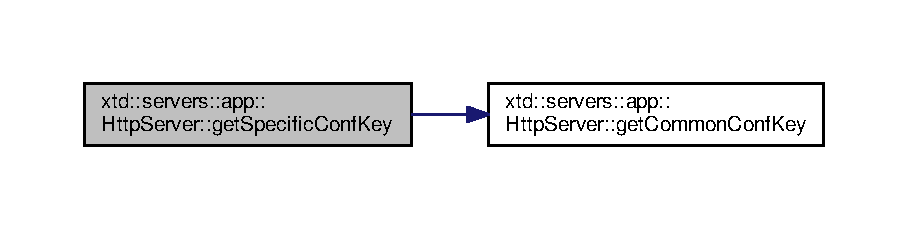
\includegraphics[width=350pt]{classxtd_1_1servers_1_1app_1_1HttpServer_a2b8fdc59d125cae41a833da5daf16d97_cgraph}
\end{center}
\end{figure}




Here is the caller graph for this function\-:
\nopagebreak
\begin{figure}[H]
\begin{center}
\leavevmode
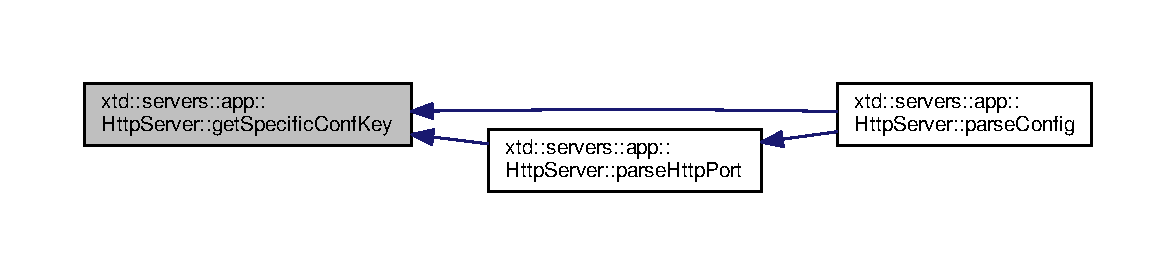
\includegraphics[width=350pt]{classxtd_1_1servers_1_1app_1_1HttpServer_a2b8fdc59d125cae41a833da5daf16d97_icgraph}
\end{center}
\end{figure}


\hypertarget{classxtd_1_1servers_1_1app_1_1HttpServer_a89a77d0dd8391a54b9560d2a32ab5ec6}{\index{xtd\-::servers\-::app\-::\-Http\-Server@{xtd\-::servers\-::app\-::\-Http\-Server}!h\-\_\-run\-Action@{h\-\_\-run\-Action}}
\index{h\-\_\-run\-Action@{h\-\_\-run\-Action}!xtd::servers::app::HttpServer@{xtd\-::servers\-::app\-::\-Http\-Server}}
\subsubsection[{h\-\_\-run\-Action}]{\setlength{\rightskip}{0pt plus 5cm}status xtd\-::servers\-::app\-::\-Http\-Server\-::h\-\_\-run\-Action (
\begin{DoxyParamCaption}
\item[{const string \&}]{p\-\_\-name, }
\item[{h}]{p\-\_\-action, }
\item[{const uint32\-\_\-t}]{p\-\_\-request\-Id, }
\item[{const network\-::http\-::\-Request \&}]{p\-\_\-req, }
\item[{network\-::http\-::\-Response \&}]{p\-\_\-res}
\end{DoxyParamCaption}
)\hspace{0.3cm}{\ttfamily [protected]}}}\label{classxtd_1_1servers_1_1app_1_1HttpServer_a89a77d0dd8391a54b9560d2a32ab5ec6}


Definition at line 329 of file Http\-Server.\-cc.


\begin{DoxyCode}
334 \{
335   status              l\_ret    = status::error;
336   \textcolor{keywordtype}{string}              l\_status = \textcolor{stringliteral}{"FAILED"};
337   \textcolor{keywordtype}{string}              l\_data;
338   http::Json          l\_tmpl;
339   \textcolor{keywordtype}{string}              l\_text;
340   t\_actions::iterator c\_action;
341 
342   c\_action = \hyperlink{classxtd_1_1servers_1_1app_1_1HttpServer_afa5363da18a3aa9de651e53e409116e9}{m\_actions}.find(p\_name);
343 
344   \textcolor{keywordflow}{if} (c\_action == \hyperlink{classxtd_1_1servers_1_1app_1_1HttpServer_afa5363da18a3aa9de651e53e409116e9}{m\_actions}.end())
345   \{
346     l\_status = \textcolor{stringliteral}{"UNKNOWN"};
347     logger::crit(\textcolor{stringliteral}{"servers.app.http"}, \textcolor{stringliteral}{"can't find action '%s' into map actions ; action aborted."}, p\_name, 
      HERE);
348   \}
349   \textcolor{keywordflow}{else}
350   \{
351     \textcolor{keywordtype}{string} l\_log;
352     p\_req.getCgi(\textcolor{stringliteral}{"log"}, l\_log);
353 
354     l\_ret = p\_action(p\_requestID, p\_req, p\_res);
355     \textcolor{keywordflow}{if} (l\_ret == status::ok)
356     \{
357       l\_status = \textcolor{stringliteral}{"DONE"};
358       p\_res.setStatus(http::code::ok);
359       c\_action->second->m\_timestamp = boost::posix\_time::microsec\_clock::local\_time();
360       c\_action->second->m\_log       = l\_log;
361     \}
362     logger::crit(\textcolor{stringliteral}{"servers.app.http"}, \textcolor{stringliteral}{"action '%s' - execution status : %s"}, p\_name, l\_status, HERE);
363   \}
364 
365   \textcolor{comment}{// Create Json response}
366   l\_tmpl.add(\textcolor{stringliteral}{"status"}, p\_name, l\_status);
367 
368   \textcolor{comment}{// Export Json to string}
369   \textcolor{keywordflow}{if} (status::ok != l\_tmpl.resolve(l\_text))
370     \textcolor{keywordflow}{return} h\_error\_text(l\_tmpl.getError(), p\_requestID, p\_req, p\_res);
371 
372   \textcolor{comment}{// Set response}
373   p\_res.addHeader(\textcolor{stringliteral}{"Content-Type"}, l\_tmpl.getContentType());
374   p\_res.setData(l\_text);
375   \textcolor{keywordflow}{return} l\_ret;
376 \}
\end{DoxyCode}


Here is the caller graph for this function\-:
\nopagebreak
\begin{figure}[H]
\begin{center}
\leavevmode
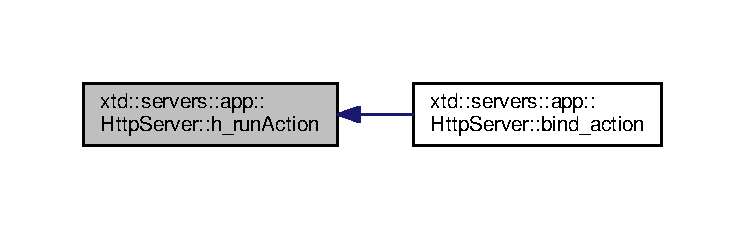
\includegraphics[width=350pt]{classxtd_1_1servers_1_1app_1_1HttpServer_a89a77d0dd8391a54b9560d2a32ab5ec6_icgraph}
\end{center}
\end{figure}


\hypertarget{classxtd_1_1servers_1_1app_1_1HttpServer_a022eecad815296f1d27b19a4b6cca908}{\index{xtd\-::servers\-::app\-::\-Http\-Server@{xtd\-::servers\-::app\-::\-Http\-Server}!handle\-T\-E\-R\-M@{handle\-T\-E\-R\-M}}
\index{handle\-T\-E\-R\-M@{handle\-T\-E\-R\-M}!xtd::servers::app::HttpServer@{xtd\-::servers\-::app\-::\-Http\-Server}}
\subsubsection[{handle\-T\-E\-R\-M}]{\setlength{\rightskip}{0pt plus 5cm}void xtd\-::servers\-::app\-::\-Http\-Server\-::handle\-T\-E\-R\-M (
\begin{DoxyParamCaption}
\item[{void}]{}
\end{DoxyParamCaption}
)\hspace{0.3cm}{\ttfamily [protected]}, {\ttfamily [virtual]}}}\label{classxtd_1_1servers_1_1app_1_1HttpServer_a022eecad815296f1d27b19a4b6cca908}


Definition at line 75 of file Http\-Server.\-cc.


\begin{DoxyCode}
76 \{
77   logger::crit(\textcolor{stringliteral}{"servers.app.http"}, \textcolor{stringliteral}{"received 'SIGTERM' signal"});
78   \hyperlink{classxtd_1_1servers_1_1app_1_1HttpServer_a7fdba08e0fa4dc9bbec30a989ccf4049}{stop}();
79 \}
\end{DoxyCode}


Here is the call graph for this function\-:
\nopagebreak
\begin{figure}[H]
\begin{center}
\leavevmode
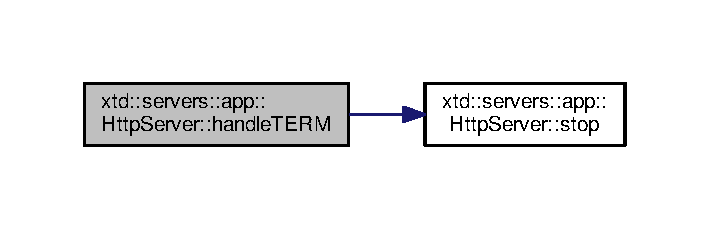
\includegraphics[width=340pt]{classxtd_1_1servers_1_1app_1_1HttpServer_a022eecad815296f1d27b19a4b6cca908_cgraph}
\end{center}
\end{figure}




Here is the caller graph for this function\-:
\nopagebreak
\begin{figure}[H]
\begin{center}
\leavevmode
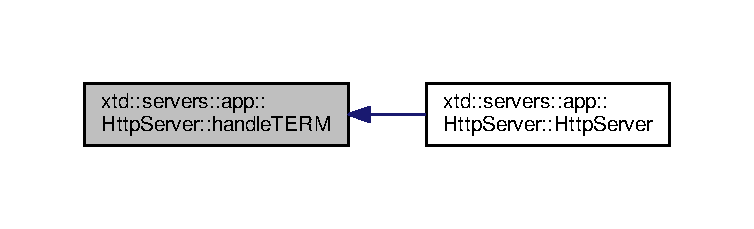
\includegraphics[width=350pt]{classxtd_1_1servers_1_1app_1_1HttpServer_a022eecad815296f1d27b19a4b6cca908_icgraph}
\end{center}
\end{figure}


\hypertarget{classxtd_1_1servers_1_1app_1_1HttpServer_a6c6bb7c70218f171e327ed2197d0f6dc}{\index{xtd\-::servers\-::app\-::\-Http\-Server@{xtd\-::servers\-::app\-::\-Http\-Server}!handle\-U\-S\-R2@{handle\-U\-S\-R2}}
\index{handle\-U\-S\-R2@{handle\-U\-S\-R2}!xtd::servers::app::HttpServer@{xtd\-::servers\-::app\-::\-Http\-Server}}
\subsubsection[{handle\-U\-S\-R2}]{\setlength{\rightskip}{0pt plus 5cm}void xtd\-::servers\-::app\-::\-Http\-Server\-::handle\-U\-S\-R2 (
\begin{DoxyParamCaption}
\item[{void}]{}
\end{DoxyParamCaption}
)\hspace{0.3cm}{\ttfamily [protected]}}}\label{classxtd_1_1servers_1_1app_1_1HttpServer_a6c6bb7c70218f171e327ed2197d0f6dc}
gestion vip hebex desactivation du service http et reponse 503 mode probe. 

Definition at line 306 of file Http\-Server.\-cc.


\begin{DoxyCode}
307 \{
308   logger::crit(\textcolor{stringliteral}{"servers.app.http"}, \textcolor{stringliteral}{"Received a 'SIGUSR2' signal : mode PROBE activated"}, HERE);
309   \hyperlink{classxtd_1_1servers_1_1app_1_1HttpServer_a4b2a904b65659aa4e5d67d1ad4a02603}{modeProbeActivation}();
310 \}
\end{DoxyCode}


Here is the call graph for this function\-:
\nopagebreak
\begin{figure}[H]
\begin{center}
\leavevmode
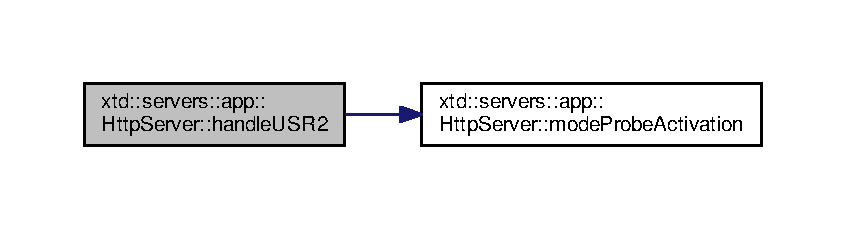
\includegraphics[width=350pt]{classxtd_1_1servers_1_1app_1_1HttpServer_a6c6bb7c70218f171e327ed2197d0f6dc_cgraph}
\end{center}
\end{figure}




Here is the caller graph for this function\-:
\nopagebreak
\begin{figure}[H]
\begin{center}
\leavevmode
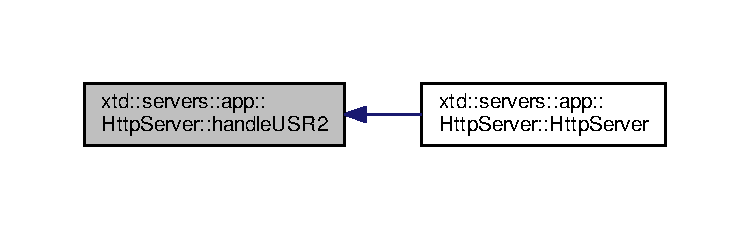
\includegraphics[width=350pt]{classxtd_1_1servers_1_1app_1_1HttpServer_a6c6bb7c70218f171e327ed2197d0f6dc_icgraph}
\end{center}
\end{figure}


\hypertarget{classxtd_1_1servers_1_1app_1_1HttpServer_a0924e53b6bc9de7563c33690d619ce9d}{\index{xtd\-::servers\-::app\-::\-Http\-Server@{xtd\-::servers\-::app\-::\-Http\-Server}!initialize@{initialize}}
\index{initialize@{initialize}!xtd::servers::app::HttpServer@{xtd\-::servers\-::app\-::\-Http\-Server}}
\subsubsection[{initialize}]{\setlength{\rightskip}{0pt plus 5cm}void xtd\-::servers\-::app\-::\-Http\-Server\-::initialize (
\begin{DoxyParamCaption}
\item[{void}]{}
\end{DoxyParamCaption}
)\hspace{0.3cm}{\ttfamily [protected]}, {\ttfamily [virtual]}}}\label{classxtd_1_1servers_1_1app_1_1HttpServer_a0924e53b6bc9de7563c33690d619ce9d}


Reimplemented in \hyperlink{classxtd_1_1servers_1_1app_1_1Server_aabde8b6a3810b09f029821dddafe3b8c}{xtd\-::servers\-::app\-::\-Server$<$ T\-Req, T\-Res, Domain $>$}.



Definition at line 240 of file Http\-Server.\-cc.


\begin{DoxyCode}
241 \{
242   \hyperlink{classxtd_1_1servers_1_1app_1_1HttpServer_a0758f122d486bc068d796d4ce550e99f}{m\_ramCounter}.reset(\textcolor{keyword}{new} counters::Value32(\textcolor{stringliteral}{"ram.usage"}));
243   \textcolor{comment}{// 60000ms = 60s = 1min : timed window size}
244   \hyperlink{classxtd_1_1servers_1_1app_1_1HttpServer_afc57d4c9bc2f9a47440e3c54eb92b1fb}{http\_app::m\_perfCounter}.reset(\textcolor{keyword}{new} counters::AvgTimedValue(\textcolor{stringliteral}{""}, 
      \hyperlink{classxtd_1_1servers_1_1app_1_1HttpServer_a2f0812d24ccfd55e943f3144c672b473}{m\_nbThread}, 60000, \hyperlink{classxtd_1_1servers_1_1app_1_1HttpServer_ad7f8a9a0475e17154850c3d575bf6f05}{m\_thresholdMs}));
245   \hyperlink{classxtd_1_1servers_1_1app_1_1HttpServer_aa26ddc958ab07774e8ba45e89dc0011b}{m\_prober}.reset(\textcolor{keyword}{new} counters::CounterManager(\hyperlink{classxtd_1_1servers_1_1app_1_1HttpServer_a87fc30b2e7e6ab2aabc2c46c884d7f17}{m\_probeDelay}, 
      \hyperlink{classxtd_1_1servers_1_1app_1_1HttpServer_affc53261a7c36873c73a06013d6b1fe6}{getSnmpPath}()));
246   \hyperlink{classxtd_1_1servers_1_1app_1_1HttpServer_ac4f9a2c40867f4f2ba8d30ec9876e51e}{m\_params}.reset(\textcolor{keyword}{new} param::Handler(\hyperlink{classxtd_1_1servers_1_1app_1_1HttpServer_ad12543f950574ac8a0d813cb4ceeff4c}{m\_adminDir}));
247 
248   \textcolor{comment}{// Link admin console contexts}
249   bind\_public(\textcolor{stringliteral}{"/admin"},    h(&HttpServer::h\_admin,      \textcolor{keyword}{this}), \textcolor{stringliteral}{"administration"});
250   bind\_public(\textcolor{stringliteral}{"/action"},   h(&HttpServer::h\_actionList, \textcolor{keyword}{this}), \textcolor{stringliteral}{"actions"});
251   bind\_public(\textcolor{stringliteral}{"/counter*"}, h(&HttpServer::h\_counter,    \textcolor{keyword}{this}), \textcolor{stringliteral}{"counters"});
252   bind\_public(\textcolor{stringliteral}{"/conf"},     h(&HttpServer::h\_conf,       \textcolor{keyword}{this}), \textcolor{stringliteral}{"configuration"});
253   bind\_public(\textcolor{stringliteral}{"/ident"},    h(&HttpServer::h\_ident,      \textcolor{keyword}{this}), \textcolor{stringliteral}{"identity"});
254   bind\_public(\textcolor{stringliteral}{"/log"},      h(&HttpServer::h\_log,        \textcolor{keyword}{this}), \textcolor{stringliteral}{"logs"});
255   bind\_public(\textcolor{stringliteral}{"/index"},    h(&HttpServer::h\_index,      \textcolor{keyword}{this}), \textcolor{stringliteral}{"index"});
256 
257 
258   bind\_dir(\textcolor{stringliteral}{"/css/images/*"}, \hyperlink{classxtd_1_1servers_1_1app_1_1HttpServer_abfb9586e84fa5149da3226eeea39980f}{m\_httpConfigPath} + \textcolor{stringliteral}{"/css/images"}, \textcolor{stringliteral}{"images/png"},      \textcolor{keyword}{true});
259   bind\_dir(\textcolor{stringliteral}{"/css/*"},        \hyperlink{classxtd_1_1servers_1_1app_1_1HttpServer_abfb9586e84fa5149da3226eeea39980f}{m\_httpConfigPath} + \textcolor{stringliteral}{"/css"},        \textcolor{stringliteral}{"text/css"},        \textcolor{keyword}{true});
260   bind\_dir(\textcolor{stringliteral}{"/img/gif/*"},    \hyperlink{classxtd_1_1servers_1_1app_1_1HttpServer_abfb9586e84fa5149da3226eeea39980f}{m\_httpConfigPath} + \textcolor{stringliteral}{"/img/gif"},    \textcolor{stringliteral}{"image/gif"},       \textcolor{keyword}{true});
261   bind\_dir(\textcolor{stringliteral}{"/img/png/*"},    \hyperlink{classxtd_1_1servers_1_1app_1_1HttpServer_abfb9586e84fa5149da3226eeea39980f}{m\_httpConfigPath} + \textcolor{stringliteral}{"/img/png"},    \textcolor{stringliteral}{"image/png"},       \textcolor{keyword}{true});
262   bind\_dir(\textcolor{stringliteral}{"/js/*"},         \hyperlink{classxtd_1_1servers_1_1app_1_1HttpServer_abfb9586e84fa5149da3226eeea39980f}{m\_httpConfigPath} + \textcolor{stringliteral}{"/js"},         \textcolor{stringliteral}{"text/javascript"}, \textcolor{keyword}{true});
263 
264   bind\_redirect(\textcolor{stringliteral}{"/"}, \textcolor{stringliteral}{"/index"});
265 
266   \textcolor{comment}{// Add mode probe handler}
267   bind\_any(h(&HttpServer::h\_probe, \textcolor{keyword}{this}),
268            f(&HttpServer::f\_cgi\_exist, \textcolor{keyword}{this}, \textcolor{stringliteral}{"mode"}) &&
269            f(&HttpServer::f\_cgi\_equal, \textcolor{keyword}{this}, \textcolor{stringliteral}{"mode"}, \textcolor{stringliteral}{"probe"}));
270 \}
\end{DoxyCode}


Here is the call graph for this function\-:
\nopagebreak
\begin{figure}[H]
\begin{center}
\leavevmode
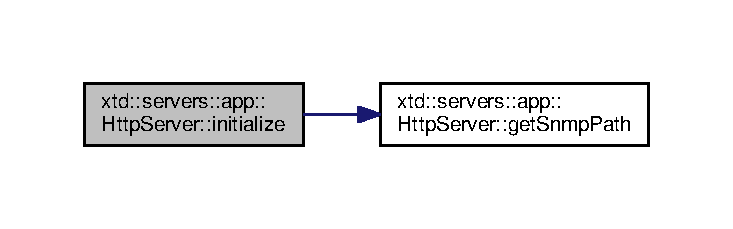
\includegraphics[width=350pt]{classxtd_1_1servers_1_1app_1_1HttpServer_a0924e53b6bc9de7563c33690d619ce9d_cgraph}
\end{center}
\end{figure}


\hypertarget{classxtd_1_1servers_1_1app_1_1HttpServer_a4b2a904b65659aa4e5d67d1ad4a02603}{\index{xtd\-::servers\-::app\-::\-Http\-Server@{xtd\-::servers\-::app\-::\-Http\-Server}!mode\-Probe\-Activation@{mode\-Probe\-Activation}}
\index{mode\-Probe\-Activation@{mode\-Probe\-Activation}!xtd::servers::app::HttpServer@{xtd\-::servers\-::app\-::\-Http\-Server}}
\subsubsection[{mode\-Probe\-Activation}]{\setlength{\rightskip}{0pt plus 5cm}void xtd\-::servers\-::app\-::\-Http\-Server\-::mode\-Probe\-Activation (
\begin{DoxyParamCaption}
\item[{void}]{}
\end{DoxyParamCaption}
)\hspace{0.3cm}{\ttfamily [protected]}}}\label{classxtd_1_1servers_1_1app_1_1HttpServer_a4b2a904b65659aa4e5d67d1ad4a02603}


Definition at line 312 of file Http\-Server.\-cc.


\begin{DoxyCode}
313 \{
314   \hyperlink{classxtd_1_1servers_1_1app_1_1HttpServer_a3ae2e35fc931b303e244b01e277cb8dd}{m\_isModeProbe} = \textcolor{keyword}{true};
315 \}
\end{DoxyCode}


Here is the caller graph for this function\-:
\nopagebreak
\begin{figure}[H]
\begin{center}
\leavevmode
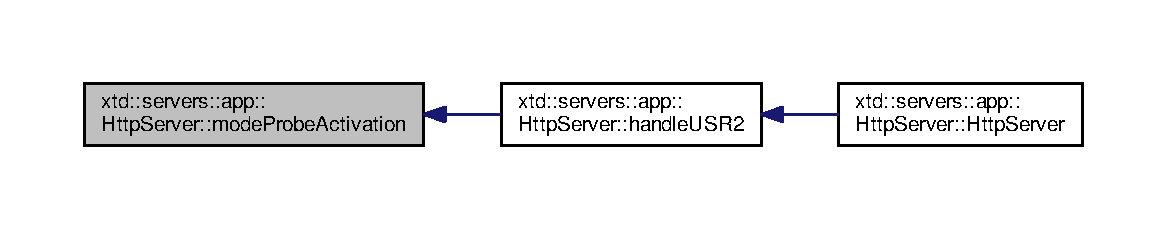
\includegraphics[width=350pt]{classxtd_1_1servers_1_1app_1_1HttpServer_a4b2a904b65659aa4e5d67d1ad4a02603_icgraph}
\end{center}
\end{figure}


\hypertarget{classxtd_1_1servers_1_1app_1_1HttpServer_af4baf6c6e7397177a20122e1f1101f9f}{\index{xtd\-::servers\-::app\-::\-Http\-Server@{xtd\-::servers\-::app\-::\-Http\-Server}!parse\-Config@{parse\-Config}}
\index{parse\-Config@{parse\-Config}!xtd::servers::app::HttpServer@{xtd\-::servers\-::app\-::\-Http\-Server}}
\subsubsection[{parse\-Config}]{\setlength{\rightskip}{0pt plus 5cm}void xtd\-::servers\-::app\-::\-Http\-Server\-::parse\-Config (
\begin{DoxyParamCaption}
\item[{void}]{}
\end{DoxyParamCaption}
)\hspace{0.3cm}{\ttfamily [protected]}, {\ttfamily [virtual]}}}\label{classxtd_1_1servers_1_1app_1_1HttpServer_af4baf6c6e7397177a20122e1f1101f9f}


Reimplemented in \hyperlink{classxtd_1_1servers_1_1app_1_1Server_a04ac2d5b3a0a229a3b54ef33b9b7056d}{xtd\-::servers\-::app\-::\-Server$<$ T\-Req, T\-Res, Domain $>$}.



Definition at line 99 of file Http\-Server.\-cc.


\begin{DoxyCode}
100 \{
101   \textcolor{keywordtype}{string}   l\_key;
102   \textcolor{keywordtype}{string}   l\_strValue;
103   \textcolor{keywordtype}{string}   l\_common    = \hyperlink{classxtd_1_1servers_1_1app_1_1HttpServer_a3c838a2599ff485454ca19790ae0529c}{getCommonConfKey}();
104   \textcolor{keywordtype}{string}   l\_specific  = \hyperlink{classxtd_1_1servers_1_1app_1_1HttpServer_a2b8fdc59d125cae41a833da5daf16d97}{getSpecificConfKey}();
105   uint32\_t l\_timeoutMs = 0;;
106 
107   \textcolor{comment}{// Retrieve configuration file}
108   \textcolor{keywordflow}{try}
109   \{
110     \textcolor{keywordflow}{if} (0 == \hyperlink{classxtd_1_1servers_1_1app_1_1HttpServer_aa07526617267875dd907e29b99711ab6}{m\_configPath}.size())
111     \{
112       error\_nohelp(1, \textcolor{stringliteral}{"option --config-file is mandatory"});
113     \}
114 
115     \textcolor{keywordflow}{if} ((\textcolor{keyword}{false} == boost::filesystem::is\_regular\_file(\hyperlink{classxtd_1_1servers_1_1app_1_1HttpServer_aa07526617267875dd907e29b99711ab6}{m\_configPath})) &&
116         (\textcolor{keyword}{false} == boost::filesystem::is\_symlink(\hyperlink{classxtd_1_1servers_1_1app_1_1HttpServer_aa07526617267875dd907e29b99711ab6}{m\_configPath})))
117     \{
118       error\_nohelp(1, \textcolor{stringliteral}{"invalid --config-file='%s' option, file unreadable"}, 
      \hyperlink{classxtd_1_1servers_1_1app_1_1HttpServer_aa07526617267875dd907e29b99711ab6}{m\_configPath});
119     \}
120 
121     \hyperlink{classxtd_1_1servers_1_1app_1_1HttpServer_ada282c895467a8d2fcaee543560958dc}{m\_config}.reset(\textcolor{keyword}{new} ConfParser(\hyperlink{classxtd_1_1servers_1_1app_1_1HttpServer_aa07526617267875dd907e29b99711ab6}{m\_configPath}));
122   \}
123   \textcolor{keywordflow}{catch} (std::exception& l\_error)
124   \{
125     error\_nohelp(1, \textcolor{stringliteral}{"could not load config file '%s' : %s"}, \hyperlink{classxtd_1_1servers_1_1app_1_1HttpServer_aa07526617267875dd907e29b99711ab6}{m\_configPath}, l\_error.what());
126   \}
127 
128 
129   \textcolor{comment}{// log level}
130   \textcolor{keywordflow}{if} (\textcolor{keyword}{false} == isOptionGiven(\textcolor{stringliteral}{"e"}))
131   \{
132     l\_key = str(format(\textcolor{stringliteral}{"%s:server:log\_level"}) % l\_common);
133     \hyperlink{classxtd_1_1servers_1_1app_1_1HttpServer_ae1cffd988b56081fba6f124e9f0743fd}{readConf}(l\_key, m\_logLevel, m\_logLevel);
134   \}
135 
136   \textcolor{comment}{// snmp path}
137   l\_key      = str(format(\textcolor{stringliteral}{"%s:server:snmp\_dir"}) % l\_common);
138   l\_strValue = str(format(\textcolor{stringliteral}{"/var/run/snmp/%s"}) % l\_common);
139   \hyperlink{classxtd_1_1servers_1_1app_1_1HttpServer_ae1cffd988b56081fba6f124e9f0743fd}{readConf}(l\_key, \hyperlink{classxtd_1_1servers_1_1app_1_1HttpServer_a555ce1e115602fda522a5c0a675dace3}{m\_snmpPath}, l\_strValue);
140 
141   \textcolor{comment}{// action dir}
142   l\_key      = str(format(\textcolor{stringliteral}{"%s:server:action\_dir"}) % l\_specific);
143   l\_strValue = str(format(\textcolor{stringliteral}{"%s/admin"}) % \hyperlink{classxtd_1_1servers_1_1app_1_1HttpServer_a555ce1e115602fda522a5c0a675dace3}{m\_snmpPath});
144   \hyperlink{classxtd_1_1servers_1_1app_1_1HttpServer_ae1cffd988b56081fba6f124e9f0743fd}{readConf}(l\_key, \hyperlink{classxtd_1_1servers_1_1app_1_1HttpServer_ad12543f950574ac8a0d813cb4ceeff4c}{m\_adminDir}, l\_strValue);
145 
146 
147   \textcolor{comment}{// refresh delay}
148   l\_key = str(format(\textcolor{stringliteral}{"%s:server:snmp\_refresh\_delay\_sec"}) % l\_common);
149   \hyperlink{classxtd_1_1servers_1_1app_1_1HttpServer_ae1cffd988b56081fba6f124e9f0743fd}{readConf}(l\_key, \hyperlink{classxtd_1_1servers_1_1app_1_1HttpServer_a87fc30b2e7e6ab2aabc2c46c884d7f17}{m\_probeDelay});
150 
151   \textcolor{comment}{// assets dir}
152   l\_key = str(format(\textcolor{stringliteral}{"%s:server:http:assets\_dir"}) % l\_common);
153   \hyperlink{classxtd_1_1servers_1_1app_1_1HttpServer_ae1cffd988b56081fba6f124e9f0743fd}{readConf}(l\_key, \hyperlink{classxtd_1_1servers_1_1app_1_1HttpServer_abfb9586e84fa5149da3226eeea39980f}{m\_httpConfigPath}, \hyperlink{classxtd_1_1servers_1_1app_1_1HttpServer_abfb9586e84fa5149da3226eeea39980f}{m\_httpConfigPath});
154 
155   \textcolor{comment}{// listen interface}
156   l\_key = str(format(\textcolor{stringliteral}{"%s:server:http:listen"}) % l\_common);
157   \hyperlink{classxtd_1_1servers_1_1app_1_1HttpServer_ae1cffd988b56081fba6f124e9f0743fd}{readConf}(l\_key, \hyperlink{classxtd_1_1servers_1_1app_1_1HttpServer_af1676247676379d0c12008bdcd5b7e17}{m\_httpHost}, \textcolor{keywordtype}{string}(
      \hyperlink{classxtd_1_1servers_1_1app_1_1HttpServer_a38433b4c2d0bba9f0bae81266b42bac1}{mcs\_defaultListenInterface}));
158 
159   \textcolor{comment}{// threads}
160   \textcolor{keywordflow}{if} (\textcolor{keyword}{false} == isOptionGiven(\textcolor{stringliteral}{"n"}))
161   \{
162     l\_key = str(format(\textcolor{stringliteral}{"%s:server:http:threads"}) % l\_common);
163     \hyperlink{classxtd_1_1servers_1_1app_1_1HttpServer_ae1cffd988b56081fba6f124e9f0743fd}{readConf}(l\_key, \hyperlink{classxtd_1_1servers_1_1app_1_1HttpServer_a2f0812d24ccfd55e943f3144c672b473}{m\_nbThread});
164   \}
165 
166   l\_key = str(format(\textcolor{stringliteral}{"%s:server:http:threshold\_ms"}) % l\_common);
167   \hyperlink{classxtd_1_1servers_1_1app_1_1HttpServer_ae1cffd988b56081fba6f124e9f0743fd}{readConf}(l\_key, \hyperlink{classxtd_1_1servers_1_1app_1_1HttpServer_ad7f8a9a0475e17154850c3d575bf6f05}{m\_thresholdMs}, \hyperlink{classxtd_1_1servers_1_1app_1_1HttpServer_ad7f8a9a0475e17154850c3d575bf6f05}{m\_thresholdMs});
168 
169   \textcolor{comment}{// http port : delegate to child class}
170   \textcolor{keywordflow}{if} (\textcolor{keyword}{false} == isOptionGiven(\textcolor{stringliteral}{"http-port"}))
171     \hyperlink{classxtd_1_1servers_1_1app_1_1HttpServer_a2b65812ed2afa6629f115b76c4ab6e41}{parseHttpPort}();
172 
173   \textcolor{comment}{// http receive timeout}
174   l\_key = str(format(\textcolor{stringliteral}{"%s:server:http:rcv\_timeout\_ms"}) % l\_common);
175   \hyperlink{classxtd_1_1servers_1_1app_1_1HttpServer_ae1cffd988b56081fba6f124e9f0743fd}{readConf}(l\_key, l\_timeoutMs, \hyperlink{classxtd_1_1servers_1_1app_1_1HttpServer_ad5f2480d758b731b641e4858f556a3c3}{m\_httpConfig}.getReceiveTimeoutMs());
176   \hyperlink{classxtd_1_1servers_1_1app_1_1HttpServer_ad5f2480d758b731b641e4858f556a3c3}{m\_httpConfig}.setReceiveTimeoutMs(l\_timeoutMs);
177 
178   \textcolor{comment}{// http send timeout ms}
179   l\_key = str(format(\textcolor{stringliteral}{"%s:server:http:send\_timeout\_ms"}) % l\_common);
180   \hyperlink{classxtd_1_1servers_1_1app_1_1HttpServer_ae1cffd988b56081fba6f124e9f0743fd}{readConf}(l\_key, l\_timeoutMs, \hyperlink{classxtd_1_1servers_1_1app_1_1HttpServer_ad5f2480d758b731b641e4858f556a3c3}{m\_httpConfig}.getSendTimeoutMs());
181   \hyperlink{classxtd_1_1servers_1_1app_1_1HttpServer_ad5f2480d758b731b641e4858f556a3c3}{m\_httpConfig}.setSendTimeoutMs(l\_timeoutMs);
182 \}
\end{DoxyCode}


Here is the call graph for this function\-:
\nopagebreak
\begin{figure}[H]
\begin{center}
\leavevmode
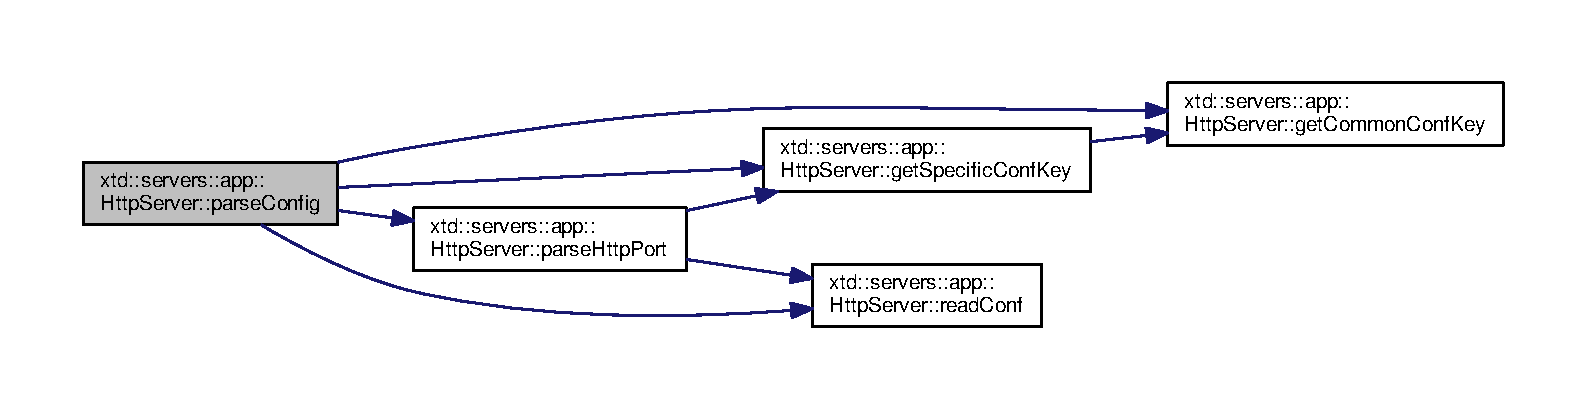
\includegraphics[width=350pt]{classxtd_1_1servers_1_1app_1_1HttpServer_af4baf6c6e7397177a20122e1f1101f9f_cgraph}
\end{center}
\end{figure}


\hypertarget{classxtd_1_1servers_1_1app_1_1HttpServer_a2b65812ed2afa6629f115b76c4ab6e41}{\index{xtd\-::servers\-::app\-::\-Http\-Server@{xtd\-::servers\-::app\-::\-Http\-Server}!parse\-Http\-Port@{parse\-Http\-Port}}
\index{parse\-Http\-Port@{parse\-Http\-Port}!xtd::servers::app::HttpServer@{xtd\-::servers\-::app\-::\-Http\-Server}}
\subsubsection[{parse\-Http\-Port}]{\setlength{\rightskip}{0pt plus 5cm}void xtd\-::servers\-::app\-::\-Http\-Server\-::parse\-Http\-Port (
\begin{DoxyParamCaption}
\item[{void}]{}
\end{DoxyParamCaption}
)\hspace{0.3cm}{\ttfamily [protected]}, {\ttfamily [virtual]}}}\label{classxtd_1_1servers_1_1app_1_1HttpServer_a2b65812ed2afa6629f115b76c4ab6e41}


Definition at line 185 of file Http\-Server.\-cc.


\begin{DoxyCode}
186 \{
187   \textcolor{keywordtype}{string} l\_key = boost::str(boost::format(\textcolor{stringliteral}{"%s:server:http:port"}) % 
      \hyperlink{classxtd_1_1servers_1_1app_1_1HttpServer_a2b8fdc59d125cae41a833da5daf16d97}{getSpecificConfKey}());
188   \hyperlink{classxtd_1_1servers_1_1app_1_1HttpServer_ae1cffd988b56081fba6f124e9f0743fd}{readConf}(l\_key, \hyperlink{classxtd_1_1servers_1_1app_1_1HttpServer_a75ed3bcfa895cad365f6bf0955efcf9e}{m\_httpPort});
189 \}
\end{DoxyCode}


Here is the call graph for this function\-:
\nopagebreak
\begin{figure}[H]
\begin{center}
\leavevmode
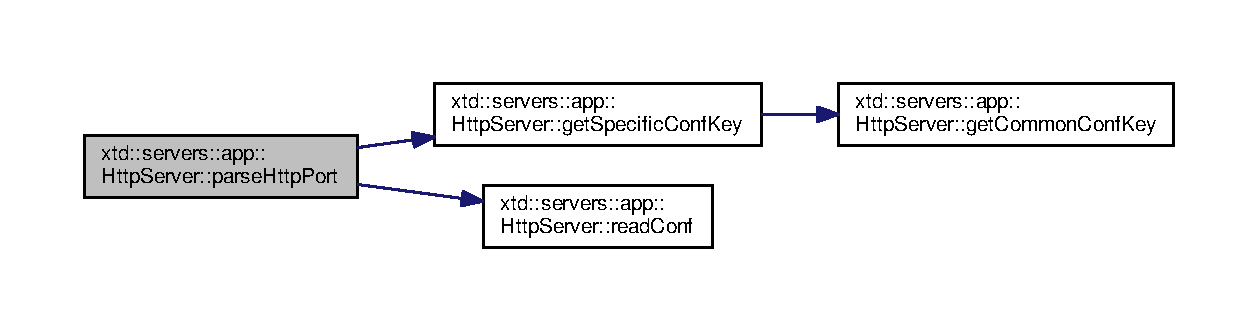
\includegraphics[width=350pt]{classxtd_1_1servers_1_1app_1_1HttpServer_a2b65812ed2afa6629f115b76c4ab6e41_cgraph}
\end{center}
\end{figure}




Here is the caller graph for this function\-:
\nopagebreak
\begin{figure}[H]
\begin{center}
\leavevmode
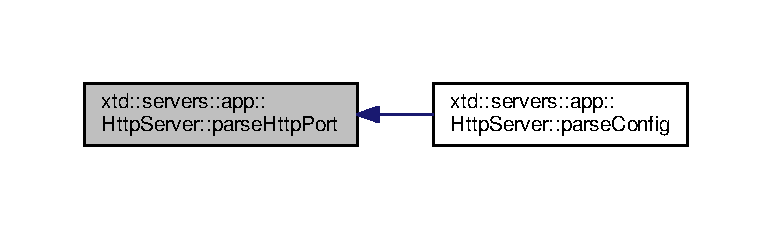
\includegraphics[width=350pt]{classxtd_1_1servers_1_1app_1_1HttpServer_a2b65812ed2afa6629f115b76c4ab6e41_icgraph}
\end{center}
\end{figure}


\hypertarget{classxtd_1_1servers_1_1app_1_1HttpServer_a2b52e7d39c3b1937a4802bf7c3d159f8}{\index{xtd\-::servers\-::app\-::\-Http\-Server@{xtd\-::servers\-::app\-::\-Http\-Server}!process@{process}}
\index{process@{process}!xtd::servers::app::HttpServer@{xtd\-::servers\-::app\-::\-Http\-Server}}
\subsubsection[{process}]{\setlength{\rightskip}{0pt plus 5cm}int xtd\-::servers\-::app\-::\-Http\-Server\-::process (
\begin{DoxyParamCaption}
\item[{void}]{}
\end{DoxyParamCaption}
)\hspace{0.3cm}{\ttfamily [protected]}, {\ttfamily [virtual]}}}\label{classxtd_1_1servers_1_1app_1_1HttpServer_a2b52e7d39c3b1937a4802bf7c3d159f8}


Definition at line 273 of file Http\-Server.\-cc.


\begin{DoxyCode}
274 \{
275   \textcolor{keywordflow}{if} (status::ok != \hyperlink{classxtd_1_1servers_1_1app_1_1HttpServer_a66c2a3b5bca8390d96b35daebfccabf3}{defineProbes}())
276     error\_nohelp(1, \textcolor{stringliteral}{"unable to create exploit probes"});
277 
278 
279   \textcolor{keywordflow}{try}
280   \{
281     \textcolor{comment}{// 1.}
282     http\_net::initialize(\hyperlink{classxtd_1_1servers_1_1app_1_1HttpServer_af1676247676379d0c12008bdcd5b7e17}{m\_httpHost}, \hyperlink{classxtd_1_1servers_1_1app_1_1HttpServer_a75ed3bcfa895cad365f6bf0955efcf9e}{m\_httpPort}, 
      \hyperlink{classxtd_1_1servers_1_1app_1_1HttpServer_ad5f2480d758b731b641e4858f556a3c3}{m\_httpConfig}, \hyperlink{classxtd_1_1servers_1_1app_1_1HttpServer_a2f0812d24ccfd55e943f3144c672b473}{m\_nbThread});
283     \textcolor{comment}{// 2.}
284     \hyperlink{classxtd_1_1servers_1_1app_1_1HttpServer_a6fac87218bf8d69ef6baeb56819411f9}{start}();
285     \textcolor{comment}{// 3.}
286     http\_net::join();
287   \}
288   \textcolor{keywordflow}{catch} (std::exception& l\_error)
289   \{
290     error\_nohelp(1, \textcolor{stringliteral}{"unable to run http server on %s:%d, %s"}, \hyperlink{classxtd_1_1servers_1_1app_1_1HttpServer_af1676247676379d0c12008bdcd5b7e17}{m\_httpHost}, 
      \hyperlink{classxtd_1_1servers_1_1app_1_1HttpServer_a75ed3bcfa895cad365f6bf0955efcf9e}{m\_httpPort}, l\_error.what());
291     \textcolor{keywordflow}{return} 1;
292   \}
293 
294   \hyperlink{classxtd_1_1servers_1_1app_1_1HttpServer_aa26ddc958ab07774e8ba45e89dc0011b}{m\_prober}->stop();
295 
296   \textcolor{keywordflow}{return} 0;
297 \}
\end{DoxyCode}


Here is the call graph for this function\-:
\nopagebreak
\begin{figure}[H]
\begin{center}
\leavevmode
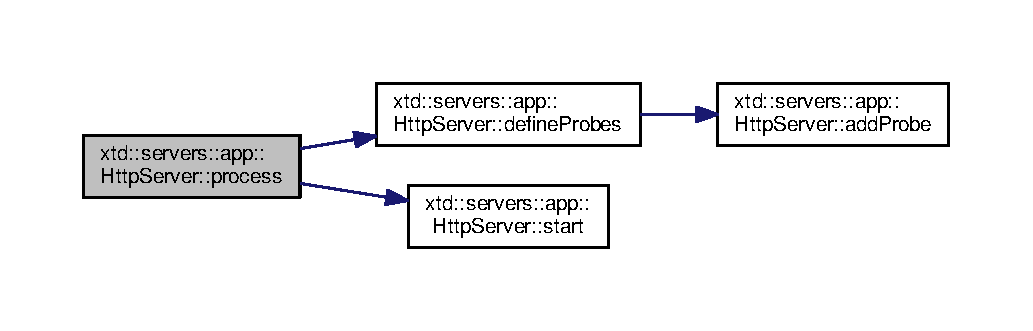
\includegraphics[width=350pt]{classxtd_1_1servers_1_1app_1_1HttpServer_a2b52e7d39c3b1937a4802bf7c3d159f8_cgraph}
\end{center}
\end{figure}


\hypertarget{classxtd_1_1servers_1_1app_1_1HttpServer_ae1cffd988b56081fba6f124e9f0743fd}{\index{xtd\-::servers\-::app\-::\-Http\-Server@{xtd\-::servers\-::app\-::\-Http\-Server}!read\-Conf@{read\-Conf}}
\index{read\-Conf@{read\-Conf}!xtd::servers::app::HttpServer@{xtd\-::servers\-::app\-::\-Http\-Server}}
\subsubsection[{read\-Conf}]{\setlength{\rightskip}{0pt plus 5cm}template$<$typename T $>$ status xtd\-::servers\-::app\-::\-Http\-Server\-::read\-Conf (
\begin{DoxyParamCaption}
\item[{const std\-::string \&}]{p\-\_\-key, }
\item[{T \&}]{p\-\_\-dst, }
\item[{const T \&}]{p\-\_\-default}
\end{DoxyParamCaption}
)\hspace{0.3cm}{\ttfamily [protected]}}}\label{classxtd_1_1servers_1_1app_1_1HttpServer_ae1cffd988b56081fba6f124e9f0743fd}


Here is the caller graph for this function\-:
\nopagebreak
\begin{figure}[H]
\begin{center}
\leavevmode
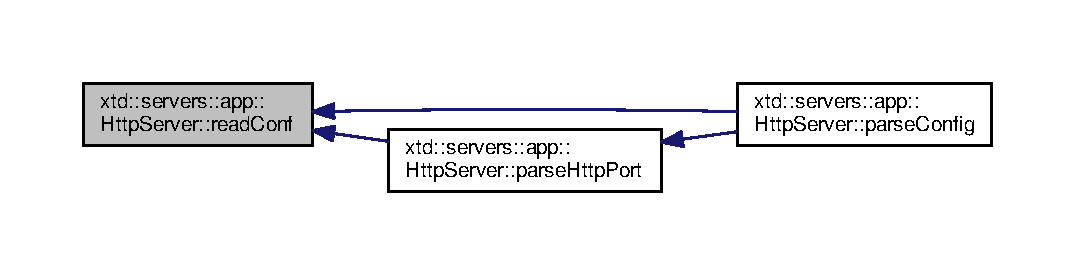
\includegraphics[width=350pt]{classxtd_1_1servers_1_1app_1_1HttpServer_ae1cffd988b56081fba6f124e9f0743fd_icgraph}
\end{center}
\end{figure}


\hypertarget{classxtd_1_1servers_1_1app_1_1HttpServer_abe54ee996274b1f6d4a89d29bba56ae8}{\index{xtd\-::servers\-::app\-::\-Http\-Server@{xtd\-::servers\-::app\-::\-Http\-Server}!read\-Conf@{read\-Conf}}
\index{read\-Conf@{read\-Conf}!xtd::servers::app::HttpServer@{xtd\-::servers\-::app\-::\-Http\-Server}}
\subsubsection[{read\-Conf}]{\setlength{\rightskip}{0pt plus 5cm}template$<$typename T $>$ status xtd\-::servers\-::app\-::\-Http\-Server\-::read\-Conf (
\begin{DoxyParamCaption}
\item[{const std\-::string \&}]{p\-\_\-key, }
\item[{T \&}]{p\-\_\-dst}
\end{DoxyParamCaption}
)\hspace{0.3cm}{\ttfamily [protected]}}}\label{classxtd_1_1servers_1_1app_1_1HttpServer_abe54ee996274b1f6d4a89d29bba56ae8}
\hypertarget{classxtd_1_1servers_1_1app_1_1HttpServer_a9247cbc7930939b40df98a20167007c3}{\index{xtd\-::servers\-::app\-::\-Http\-Server@{xtd\-::servers\-::app\-::\-Http\-Server}!set\-Last\-Admin\-Log@{set\-Last\-Admin\-Log}}
\index{set\-Last\-Admin\-Log@{set\-Last\-Admin\-Log}!xtd::servers::app::HttpServer@{xtd\-::servers\-::app\-::\-Http\-Server}}
\subsubsection[{set\-Last\-Admin\-Log}]{\setlength{\rightskip}{0pt plus 5cm}void xtd\-::servers\-::app\-::\-Http\-Server\-::set\-Last\-Admin\-Log (
\begin{DoxyParamCaption}
\item[{const string \&}]{p\-\_\-message}
\end{DoxyParamCaption}
)\hspace{0.3cm}{\ttfamily [protected]}}}\label{classxtd_1_1servers_1_1app_1_1HttpServer_a9247cbc7930939b40df98a20167007c3}
\hypertarget{classxtd_1_1servers_1_1app_1_1HttpServer_a6fac87218bf8d69ef6baeb56819411f9}{\index{xtd\-::servers\-::app\-::\-Http\-Server@{xtd\-::servers\-::app\-::\-Http\-Server}!start@{start}}
\index{start@{start}!xtd::servers::app::HttpServer@{xtd\-::servers\-::app\-::\-Http\-Server}}
\subsubsection[{start}]{\setlength{\rightskip}{0pt plus 5cm}void xtd\-::servers\-::app\-::\-Http\-Server\-::start (
\begin{DoxyParamCaption}
\item[{void}]{}
\end{DoxyParamCaption}
)\hspace{0.3cm}{\ttfamily [protected]}, {\ttfamily [virtual]}}}\label{classxtd_1_1servers_1_1app_1_1HttpServer_a6fac87218bf8d69ef6baeb56819411f9}


Reimplemented in \hyperlink{classxtd_1_1servers_1_1app_1_1Server_a8e21bf6e7993a2e04fd70d0ce88ca487}{xtd\-::servers\-::app\-::\-Server$<$ T\-Req, T\-Res, Domain $>$}.



Definition at line 82 of file Http\-Server.\-cc.


\begin{DoxyCode}
83 \{
84   \hyperlink{classxtd_1_1servers_1_1app_1_1HttpServer_ac4f9a2c40867f4f2ba8d30ec9876e51e}{m\_params}->initialize();
85   \hyperlink{classxtd_1_1servers_1_1app_1_1HttpServer_aa26ddc958ab07774e8ba45e89dc0011b}{m\_prober}->start();
86   http\_net::start();
87   logger::crit(\textcolor{stringliteral}{"servers.app.http"}, \textcolor{stringliteral}{"app::http server started"});
88 \}
\end{DoxyCode}


Here is the caller graph for this function\-:
\nopagebreak
\begin{figure}[H]
\begin{center}
\leavevmode
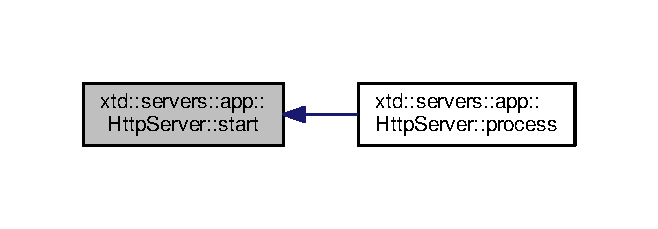
\includegraphics[width=316pt]{classxtd_1_1servers_1_1app_1_1HttpServer_a6fac87218bf8d69ef6baeb56819411f9_icgraph}
\end{center}
\end{figure}


\hypertarget{classxtd_1_1servers_1_1app_1_1HttpServer_a7fdba08e0fa4dc9bbec30a989ccf4049}{\index{xtd\-::servers\-::app\-::\-Http\-Server@{xtd\-::servers\-::app\-::\-Http\-Server}!stop@{stop}}
\index{stop@{stop}!xtd::servers::app::HttpServer@{xtd\-::servers\-::app\-::\-Http\-Server}}
\subsubsection[{stop}]{\setlength{\rightskip}{0pt plus 5cm}void xtd\-::servers\-::app\-::\-Http\-Server\-::stop (
\begin{DoxyParamCaption}
\item[{void}]{}
\end{DoxyParamCaption}
)\hspace{0.3cm}{\ttfamily [protected]}, {\ttfamily [virtual]}}}\label{classxtd_1_1servers_1_1app_1_1HttpServer_a7fdba08e0fa4dc9bbec30a989ccf4049}


Reimplemented in \hyperlink{classxtd_1_1servers_1_1app_1_1Server_a37fe0eca660f81a9edde0c1ce6938f39}{xtd\-::servers\-::app\-::\-Server$<$ T\-Req, T\-Res, Domain $>$}.



Definition at line 91 of file Http\-Server.\-cc.


\begin{DoxyCode}
92 \{
93   http\_net::stop();
94   logger::crit(\textcolor{stringliteral}{"servers.app.http"}, \textcolor{stringliteral}{"app::http server stopped"});
95   \hyperlink{classxtd_1_1servers_1_1app_1_1HttpServer_aa26ddc958ab07774e8ba45e89dc0011b}{m\_prober}->stop();
96 \}
\end{DoxyCode}


Here is the caller graph for this function\-:
\nopagebreak
\begin{figure}[H]
\begin{center}
\leavevmode
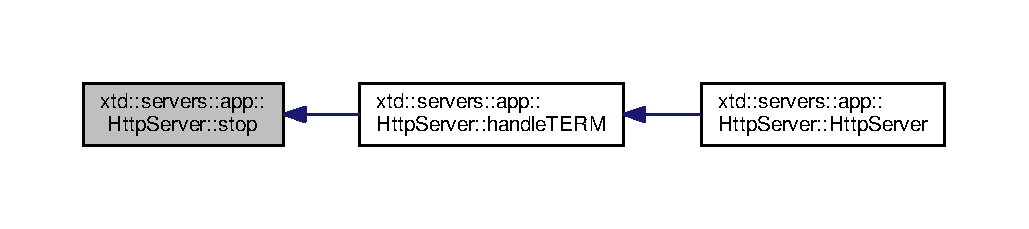
\includegraphics[width=350pt]{classxtd_1_1servers_1_1app_1_1HttpServer_a7fdba08e0fa4dc9bbec30a989ccf4049_icgraph}
\end{center}
\end{figure}




\subsection{Member Data Documentation}
\hypertarget{classxtd_1_1servers_1_1app_1_1HttpServer_afa5363da18a3aa9de651e53e409116e9}{\index{xtd\-::servers\-::app\-::\-Http\-Server@{xtd\-::servers\-::app\-::\-Http\-Server}!m\-\_\-actions@{m\-\_\-actions}}
\index{m\-\_\-actions@{m\-\_\-actions}!xtd::servers::app::HttpServer@{xtd\-::servers\-::app\-::\-Http\-Server}}
\subsubsection[{m\-\_\-actions}]{\setlength{\rightskip}{0pt plus 5cm}{\bf t\-\_\-actions} xtd\-::servers\-::app\-::\-Http\-Server\-::m\-\_\-actions\hspace{0.3cm}{\ttfamily [protected]}}}\label{classxtd_1_1servers_1_1app_1_1HttpServer_afa5363da18a3aa9de651e53e409116e9}


Definition at line 197 of file Http\-Server.\-hh.

\hypertarget{classxtd_1_1servers_1_1app_1_1HttpServer_ad12543f950574ac8a0d813cb4ceeff4c}{\index{xtd\-::servers\-::app\-::\-Http\-Server@{xtd\-::servers\-::app\-::\-Http\-Server}!m\-\_\-admin\-Dir@{m\-\_\-admin\-Dir}}
\index{m\-\_\-admin\-Dir@{m\-\_\-admin\-Dir}!xtd::servers::app::HttpServer@{xtd\-::servers\-::app\-::\-Http\-Server}}
\subsubsection[{m\-\_\-admin\-Dir}]{\setlength{\rightskip}{0pt plus 5cm}string xtd\-::servers\-::app\-::\-Http\-Server\-::m\-\_\-admin\-Dir\hspace{0.3cm}{\ttfamily [protected]}}}\label{classxtd_1_1servers_1_1app_1_1HttpServer_ad12543f950574ac8a0d813cb4ceeff4c}


Definition at line 196 of file Http\-Server.\-hh.

\hypertarget{classxtd_1_1servers_1_1app_1_1HttpServer_ada282c895467a8d2fcaee543560958dc}{\index{xtd\-::servers\-::app\-::\-Http\-Server@{xtd\-::servers\-::app\-::\-Http\-Server}!m\-\_\-config@{m\-\_\-config}}
\index{m\-\_\-config@{m\-\_\-config}!xtd::servers::app::HttpServer@{xtd\-::servers\-::app\-::\-Http\-Server}}
\subsubsection[{m\-\_\-config}]{\setlength{\rightskip}{0pt plus 5cm}Conf\-Parser\-::t\-\_\-sptr xtd\-::servers\-::app\-::\-Http\-Server\-::m\-\_\-config\hspace{0.3cm}{\ttfamily [protected]}}}\label{classxtd_1_1servers_1_1app_1_1HttpServer_ada282c895467a8d2fcaee543560958dc}


Definition at line 173 of file Http\-Server.\-hh.

\hypertarget{classxtd_1_1servers_1_1app_1_1HttpServer_aa07526617267875dd907e29b99711ab6}{\index{xtd\-::servers\-::app\-::\-Http\-Server@{xtd\-::servers\-::app\-::\-Http\-Server}!m\-\_\-config\-Path@{m\-\_\-config\-Path}}
\index{m\-\_\-config\-Path@{m\-\_\-config\-Path}!xtd::servers::app::HttpServer@{xtd\-::servers\-::app\-::\-Http\-Server}}
\subsubsection[{m\-\_\-config\-Path}]{\setlength{\rightskip}{0pt plus 5cm}string xtd\-::servers\-::app\-::\-Http\-Server\-::m\-\_\-config\-Path\hspace{0.3cm}{\ttfamily [protected]}}}\label{classxtd_1_1servers_1_1app_1_1HttpServer_aa07526617267875dd907e29b99711ab6}


Definition at line 174 of file Http\-Server.\-hh.

\hypertarget{classxtd_1_1servers_1_1app_1_1HttpServer_ad5f2480d758b731b641e4858f556a3c3}{\index{xtd\-::servers\-::app\-::\-Http\-Server@{xtd\-::servers\-::app\-::\-Http\-Server}!m\-\_\-http\-Config@{m\-\_\-http\-Config}}
\index{m\-\_\-http\-Config@{m\-\_\-http\-Config}!xtd::servers::app::HttpServer@{xtd\-::servers\-::app\-::\-Http\-Server}}
\subsubsection[{m\-\_\-http\-Config}]{\setlength{\rightskip}{0pt plus 5cm}network\-::utils\-::\-Config xtd\-::servers\-::app\-::\-Http\-Server\-::m\-\_\-http\-Config\hspace{0.3cm}{\ttfamily [protected]}}}\label{classxtd_1_1servers_1_1app_1_1HttpServer_ad5f2480d758b731b641e4858f556a3c3}


Definition at line 191 of file Http\-Server.\-hh.

\hypertarget{classxtd_1_1servers_1_1app_1_1HttpServer_abfb9586e84fa5149da3226eeea39980f}{\index{xtd\-::servers\-::app\-::\-Http\-Server@{xtd\-::servers\-::app\-::\-Http\-Server}!m\-\_\-http\-Config\-Path@{m\-\_\-http\-Config\-Path}}
\index{m\-\_\-http\-Config\-Path@{m\-\_\-http\-Config\-Path}!xtd::servers::app::HttpServer@{xtd\-::servers\-::app\-::\-Http\-Server}}
\subsubsection[{m\-\_\-http\-Config\-Path}]{\setlength{\rightskip}{0pt plus 5cm}string xtd\-::servers\-::app\-::\-Http\-Server\-::m\-\_\-http\-Config\-Path\hspace{0.3cm}{\ttfamily [protected]}}}\label{classxtd_1_1servers_1_1app_1_1HttpServer_abfb9586e84fa5149da3226eeea39980f}


Definition at line 192 of file Http\-Server.\-hh.

\hypertarget{classxtd_1_1servers_1_1app_1_1HttpServer_af1676247676379d0c12008bdcd5b7e17}{\index{xtd\-::servers\-::app\-::\-Http\-Server@{xtd\-::servers\-::app\-::\-Http\-Server}!m\-\_\-http\-Host@{m\-\_\-http\-Host}}
\index{m\-\_\-http\-Host@{m\-\_\-http\-Host}!xtd::servers::app::HttpServer@{xtd\-::servers\-::app\-::\-Http\-Server}}
\subsubsection[{m\-\_\-http\-Host}]{\setlength{\rightskip}{0pt plus 5cm}string xtd\-::servers\-::app\-::\-Http\-Server\-::m\-\_\-http\-Host\hspace{0.3cm}{\ttfamily [protected]}}}\label{classxtd_1_1servers_1_1app_1_1HttpServer_af1676247676379d0c12008bdcd5b7e17}


Definition at line 189 of file Http\-Server.\-hh.

\hypertarget{classxtd_1_1servers_1_1app_1_1HttpServer_a75ed3bcfa895cad365f6bf0955efcf9e}{\index{xtd\-::servers\-::app\-::\-Http\-Server@{xtd\-::servers\-::app\-::\-Http\-Server}!m\-\_\-http\-Port@{m\-\_\-http\-Port}}
\index{m\-\_\-http\-Port@{m\-\_\-http\-Port}!xtd::servers::app::HttpServer@{xtd\-::servers\-::app\-::\-Http\-Server}}
\subsubsection[{m\-\_\-http\-Port}]{\setlength{\rightskip}{0pt plus 5cm}uint32\-\_\-t xtd\-::servers\-::app\-::\-Http\-Server\-::m\-\_\-http\-Port\hspace{0.3cm}{\ttfamily [protected]}}}\label{classxtd_1_1servers_1_1app_1_1HttpServer_a75ed3bcfa895cad365f6bf0955efcf9e}


Definition at line 190 of file Http\-Server.\-hh.

\hypertarget{classxtd_1_1servers_1_1app_1_1HttpServer_ae8b1e546b8f464e0a18c6b737ed82df8}{\index{xtd\-::servers\-::app\-::\-Http\-Server@{xtd\-::servers\-::app\-::\-Http\-Server}!m\-\_\-is\-Debug@{m\-\_\-is\-Debug}}
\index{m\-\_\-is\-Debug@{m\-\_\-is\-Debug}!xtd::servers::app::HttpServer@{xtd\-::servers\-::app\-::\-Http\-Server}}
\subsubsection[{m\-\_\-is\-Debug}]{\setlength{\rightskip}{0pt plus 5cm}bool xtd\-::servers\-::app\-::\-Http\-Server\-::m\-\_\-is\-Debug\hspace{0.3cm}{\ttfamily [protected]}}}\label{classxtd_1_1servers_1_1app_1_1HttpServer_ae8b1e546b8f464e0a18c6b737ed82df8}


Definition at line 178 of file Http\-Server.\-hh.

\hypertarget{classxtd_1_1servers_1_1app_1_1HttpServer_a3ae2e35fc931b303e244b01e277cb8dd}{\index{xtd\-::servers\-::app\-::\-Http\-Server@{xtd\-::servers\-::app\-::\-Http\-Server}!m\-\_\-is\-Mode\-Probe@{m\-\_\-is\-Mode\-Probe}}
\index{m\-\_\-is\-Mode\-Probe@{m\-\_\-is\-Mode\-Probe}!xtd::servers::app::HttpServer@{xtd\-::servers\-::app\-::\-Http\-Server}}
\subsubsection[{m\-\_\-is\-Mode\-Probe}]{\setlength{\rightskip}{0pt plus 5cm}bool xtd\-::servers\-::app\-::\-Http\-Server\-::m\-\_\-is\-Mode\-Probe\hspace{0.3cm}{\ttfamily [protected]}}}\label{classxtd_1_1servers_1_1app_1_1HttpServer_a3ae2e35fc931b303e244b01e277cb8dd}


Definition at line 177 of file Http\-Server.\-hh.

\hypertarget{classxtd_1_1servers_1_1app_1_1HttpServer_a2f0812d24ccfd55e943f3144c672b473}{\index{xtd\-::servers\-::app\-::\-Http\-Server@{xtd\-::servers\-::app\-::\-Http\-Server}!m\-\_\-nb\-Thread@{m\-\_\-nb\-Thread}}
\index{m\-\_\-nb\-Thread@{m\-\_\-nb\-Thread}!xtd::servers::app::HttpServer@{xtd\-::servers\-::app\-::\-Http\-Server}}
\subsubsection[{m\-\_\-nb\-Thread}]{\setlength{\rightskip}{0pt plus 5cm}size\-\_\-t xtd\-::servers\-::app\-::\-Http\-Server\-::m\-\_\-nb\-Thread\hspace{0.3cm}{\ttfamily [protected]}}}\label{classxtd_1_1servers_1_1app_1_1HttpServer_a2f0812d24ccfd55e943f3144c672b473}


Definition at line 175 of file Http\-Server.\-hh.

\hypertarget{classxtd_1_1servers_1_1app_1_1HttpServer_ac4f9a2c40867f4f2ba8d30ec9876e51e}{\index{xtd\-::servers\-::app\-::\-Http\-Server@{xtd\-::servers\-::app\-::\-Http\-Server}!m\-\_\-params@{m\-\_\-params}}
\index{m\-\_\-params@{m\-\_\-params}!xtd::servers::app::HttpServer@{xtd\-::servers\-::app\-::\-Http\-Server}}
\subsubsection[{m\-\_\-params}]{\setlength{\rightskip}{0pt plus 5cm}{\bf t\-\_\-param\-\_\-handler} xtd\-::servers\-::app\-::\-Http\-Server\-::m\-\_\-params\hspace{0.3cm}{\ttfamily [protected]}}}\label{classxtd_1_1servers_1_1app_1_1HttpServer_ac4f9a2c40867f4f2ba8d30ec9876e51e}


Definition at line 195 of file Http\-Server.\-hh.

\hypertarget{classxtd_1_1servers_1_1app_1_1HttpServer_afc57d4c9bc2f9a47440e3c54eb92b1fb}{\index{xtd\-::servers\-::app\-::\-Http\-Server@{xtd\-::servers\-::app\-::\-Http\-Server}!m\-\_\-perf\-Counter@{m\-\_\-perf\-Counter}}
\index{m\-\_\-perf\-Counter@{m\-\_\-perf\-Counter}!xtd::servers::app::HttpServer@{xtd\-::servers\-::app\-::\-Http\-Server}}
\subsubsection[{m\-\_\-perf\-Counter}]{\setlength{\rightskip}{0pt plus 5cm}counters\-::\-Avg\-Timed\-Value\-::t\-\_\-sptr xtd\-::servers\-::app\-::\-Http\-Server\-::m\-\_\-perf\-Counter\hspace{0.3cm}{\ttfamily [protected]}}}\label{classxtd_1_1servers_1_1app_1_1HttpServer_afc57d4c9bc2f9a47440e3c54eb92b1fb}


Definition at line 185 of file Http\-Server.\-hh.

\hypertarget{classxtd_1_1servers_1_1app_1_1HttpServer_a87fc30b2e7e6ab2aabc2c46c884d7f17}{\index{xtd\-::servers\-::app\-::\-Http\-Server@{xtd\-::servers\-::app\-::\-Http\-Server}!m\-\_\-probe\-Delay@{m\-\_\-probe\-Delay}}
\index{m\-\_\-probe\-Delay@{m\-\_\-probe\-Delay}!xtd::servers::app::HttpServer@{xtd\-::servers\-::app\-::\-Http\-Server}}
\subsubsection[{m\-\_\-probe\-Delay}]{\setlength{\rightskip}{0pt plus 5cm}uint32\-\_\-t xtd\-::servers\-::app\-::\-Http\-Server\-::m\-\_\-probe\-Delay\hspace{0.3cm}{\ttfamily [protected]}}}\label{classxtd_1_1servers_1_1app_1_1HttpServer_a87fc30b2e7e6ab2aabc2c46c884d7f17}


Definition at line 182 of file Http\-Server.\-hh.

\hypertarget{classxtd_1_1servers_1_1app_1_1HttpServer_aa26ddc958ab07774e8ba45e89dc0011b}{\index{xtd\-::servers\-::app\-::\-Http\-Server@{xtd\-::servers\-::app\-::\-Http\-Server}!m\-\_\-prober@{m\-\_\-prober}}
\index{m\-\_\-prober@{m\-\_\-prober}!xtd::servers::app::HttpServer@{xtd\-::servers\-::app\-::\-Http\-Server}}
\subsubsection[{m\-\_\-prober}]{\setlength{\rightskip}{0pt plus 5cm}{\bf t\-\_\-prober} xtd\-::servers\-::app\-::\-Http\-Server\-::m\-\_\-prober\hspace{0.3cm}{\ttfamily [protected]}}}\label{classxtd_1_1servers_1_1app_1_1HttpServer_aa26ddc958ab07774e8ba45e89dc0011b}


Definition at line 183 of file Http\-Server.\-hh.

\hypertarget{classxtd_1_1servers_1_1app_1_1HttpServer_a0758f122d486bc068d796d4ce550e99f}{\index{xtd\-::servers\-::app\-::\-Http\-Server@{xtd\-::servers\-::app\-::\-Http\-Server}!m\-\_\-ram\-Counter@{m\-\_\-ram\-Counter}}
\index{m\-\_\-ram\-Counter@{m\-\_\-ram\-Counter}!xtd::servers::app::HttpServer@{xtd\-::servers\-::app\-::\-Http\-Server}}
\subsubsection[{m\-\_\-ram\-Counter}]{\setlength{\rightskip}{0pt plus 5cm}counters\-::\-Value32\-::t\-\_\-sptr xtd\-::servers\-::app\-::\-Http\-Server\-::m\-\_\-ram\-Counter\hspace{0.3cm}{\ttfamily [protected]}}}\label{classxtd_1_1servers_1_1app_1_1HttpServer_a0758f122d486bc068d796d4ce550e99f}


Definition at line 184 of file Http\-Server.\-hh.

\hypertarget{classxtd_1_1servers_1_1app_1_1HttpServer_a555ce1e115602fda522a5c0a675dace3}{\index{xtd\-::servers\-::app\-::\-Http\-Server@{xtd\-::servers\-::app\-::\-Http\-Server}!m\-\_\-snmp\-Path@{m\-\_\-snmp\-Path}}
\index{m\-\_\-snmp\-Path@{m\-\_\-snmp\-Path}!xtd::servers::app::HttpServer@{xtd\-::servers\-::app\-::\-Http\-Server}}
\subsubsection[{m\-\_\-snmp\-Path}]{\setlength{\rightskip}{0pt plus 5cm}string xtd\-::servers\-::app\-::\-Http\-Server\-::m\-\_\-snmp\-Path\hspace{0.3cm}{\ttfamily [protected]}}}\label{classxtd_1_1servers_1_1app_1_1HttpServer_a555ce1e115602fda522a5c0a675dace3}


Definition at line 181 of file Http\-Server.\-hh.

\hypertarget{classxtd_1_1servers_1_1app_1_1HttpServer_ad7f8a9a0475e17154850c3d575bf6f05}{\index{xtd\-::servers\-::app\-::\-Http\-Server@{xtd\-::servers\-::app\-::\-Http\-Server}!m\-\_\-threshold\-Ms@{m\-\_\-threshold\-Ms}}
\index{m\-\_\-threshold\-Ms@{m\-\_\-threshold\-Ms}!xtd::servers::app::HttpServer@{xtd\-::servers\-::app\-::\-Http\-Server}}
\subsubsection[{m\-\_\-threshold\-Ms}]{\setlength{\rightskip}{0pt plus 5cm}uint32\-\_\-t xtd\-::servers\-::app\-::\-Http\-Server\-::m\-\_\-threshold\-Ms\hspace{0.3cm}{\ttfamily [protected]}}}\label{classxtd_1_1servers_1_1app_1_1HttpServer_ad7f8a9a0475e17154850c3d575bf6f05}


Definition at line 186 of file Http\-Server.\-hh.

\hypertarget{classxtd_1_1servers_1_1app_1_1HttpServer_adcaefcc003e9503dbe6ebea90bf70ef7}{\index{xtd\-::servers\-::app\-::\-Http\-Server@{xtd\-::servers\-::app\-::\-Http\-Server}!m\-\_\-timeout\-Ms@{m\-\_\-timeout\-Ms}}
\index{m\-\_\-timeout\-Ms@{m\-\_\-timeout\-Ms}!xtd::servers::app::HttpServer@{xtd\-::servers\-::app\-::\-Http\-Server}}
\subsubsection[{m\-\_\-timeout\-Ms}]{\setlength{\rightskip}{0pt plus 5cm}size\-\_\-t xtd\-::servers\-::app\-::\-Http\-Server\-::m\-\_\-timeout\-Ms\hspace{0.3cm}{\ttfamily [protected]}}}\label{classxtd_1_1servers_1_1app_1_1HttpServer_adcaefcc003e9503dbe6ebea90bf70ef7}


Definition at line 176 of file Http\-Server.\-hh.

\hypertarget{classxtd_1_1servers_1_1app_1_1HttpServer_a38433b4c2d0bba9f0bae81266b42bac1}{\index{xtd\-::servers\-::app\-::\-Http\-Server@{xtd\-::servers\-::app\-::\-Http\-Server}!mcs\-\_\-default\-Listen\-Interface@{mcs\-\_\-default\-Listen\-Interface}}
\index{mcs\-\_\-default\-Listen\-Interface@{mcs\-\_\-default\-Listen\-Interface}!xtd::servers::app::HttpServer@{xtd\-::servers\-::app\-::\-Http\-Server}}
\subsubsection[{mcs\-\_\-default\-Listen\-Interface}]{\setlength{\rightskip}{0pt plus 5cm}const char xtd\-::servers\-::app\-::\-Http\-Server\-::mcs\-\_\-default\-Listen\-Interface = \char`\"{}0.\-0.\-0.\-0\char`\"{}\hspace{0.3cm}{\ttfamily [static]}}}\label{classxtd_1_1servers_1_1app_1_1HttpServer_a38433b4c2d0bba9f0bae81266b42bac1}


Definition at line 76 of file Http\-Server.\-hh.

\hypertarget{classxtd_1_1servers_1_1app_1_1HttpServer_a9ca36e61f5c201a51a68b3919e0badb7}{\index{xtd\-::servers\-::app\-::\-Http\-Server@{xtd\-::servers\-::app\-::\-Http\-Server}!mcs\-\_\-default\-Probe\-Delay@{mcs\-\_\-default\-Probe\-Delay}}
\index{mcs\-\_\-default\-Probe\-Delay@{mcs\-\_\-default\-Probe\-Delay}!xtd::servers::app::HttpServer@{xtd\-::servers\-::app\-::\-Http\-Server}}
\subsubsection[{mcs\-\_\-default\-Probe\-Delay}]{\setlength{\rightskip}{0pt plus 5cm}const uint32\-\_\-t xtd\-::servers\-::app\-::\-Http\-Server\-::mcs\-\_\-default\-Probe\-Delay = 30\hspace{0.3cm}{\ttfamily [static]}}}\label{classxtd_1_1servers_1_1app_1_1HttpServer_a9ca36e61f5c201a51a68b3919e0badb7}


Definition at line 73 of file Http\-Server.\-hh.

\hypertarget{classxtd_1_1servers_1_1app_1_1HttpServer_ad21741083478d35b92ba0b1da7499950}{\index{xtd\-::servers\-::app\-::\-Http\-Server@{xtd\-::servers\-::app\-::\-Http\-Server}!mcs\-\_\-default\-Threshold\-Ms@{mcs\-\_\-default\-Threshold\-Ms}}
\index{mcs\-\_\-default\-Threshold\-Ms@{mcs\-\_\-default\-Threshold\-Ms}!xtd::servers::app::HttpServer@{xtd\-::servers\-::app\-::\-Http\-Server}}
\subsubsection[{mcs\-\_\-default\-Threshold\-Ms}]{\setlength{\rightskip}{0pt plus 5cm}const uint32\-\_\-t xtd\-::servers\-::app\-::\-Http\-Server\-::mcs\-\_\-default\-Threshold\-Ms = 0\hspace{0.3cm}{\ttfamily [static]}}}\label{classxtd_1_1servers_1_1app_1_1HttpServer_ad21741083478d35b92ba0b1da7499950}


Definition at line 75 of file Http\-Server.\-hh.

\hypertarget{classxtd_1_1servers_1_1app_1_1HttpServer_abdc02697ffc7fa9f8f88252101b5d1b9}{\index{xtd\-::servers\-::app\-::\-Http\-Server@{xtd\-::servers\-::app\-::\-Http\-Server}!mcs\-\_\-default\-Timeout\-Ms@{mcs\-\_\-default\-Timeout\-Ms}}
\index{mcs\-\_\-default\-Timeout\-Ms@{mcs\-\_\-default\-Timeout\-Ms}!xtd::servers::app::HttpServer@{xtd\-::servers\-::app\-::\-Http\-Server}}
\subsubsection[{mcs\-\_\-default\-Timeout\-Ms}]{\setlength{\rightskip}{0pt plus 5cm}const uint32\-\_\-t xtd\-::servers\-::app\-::\-Http\-Server\-::mcs\-\_\-default\-Timeout\-Ms = 5000\hspace{0.3cm}{\ttfamily [static]}}}\label{classxtd_1_1servers_1_1app_1_1HttpServer_abdc02697ffc7fa9f8f88252101b5d1b9}


Definition at line 74 of file Http\-Server.\-hh.



The documentation for this class was generated from the following files\-:\begin{DoxyCompactItemize}
\item 
/home/travis/build/psycofdj/xtdcpp/servers/src/app/\hyperlink{HttpServer_8hh}{Http\-Server.\-hh}\item 
/home/travis/build/psycofdj/xtdcpp/servers/src/app/\hyperlink{HttpServer_8cc}{Http\-Server.\-cc}\end{DoxyCompactItemize}

\hypertarget{classxtd_1_1servers_1_1param_1_1JsonVisitor}{}\section{xtd\+:\+:servers\+:\+:param\+:\+:Json\+Visitor Class Reference}
\label{classxtd_1_1servers_1_1param_1_1JsonVisitor}\index{xtd\+::servers\+::param\+::\+Json\+Visitor@{xtd\+::servers\+::param\+::\+Json\+Visitor}}


Json specific visitor.  




{\ttfamily \#include $<$Visitor.\+hh$>$}



Inheritance diagram for xtd\+:\+:servers\+:\+:param\+:\+:Json\+Visitor\+:
\nopagebreak
\begin{figure}[H]
\begin{center}
\leavevmode
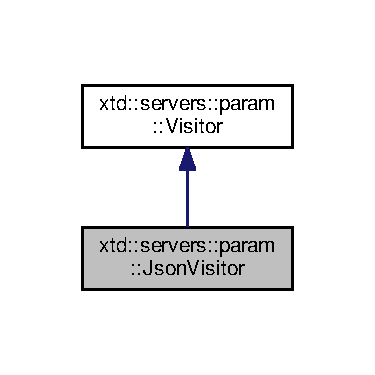
\includegraphics[width=181pt]{classxtd_1_1servers_1_1param_1_1JsonVisitor__inherit__graph}
\end{center}
\end{figure}


Collaboration diagram for xtd\+:\+:servers\+:\+:param\+:\+:Json\+Visitor\+:
\nopagebreak
\begin{figure}[H]
\begin{center}
\leavevmode
\includegraphics[width=181pt]{classxtd_1_1servers_1_1param_1_1JsonVisitor__coll__graph}
\end{center}
\end{figure}
\subsection*{Public Member Functions}
\begin{DoxyCompactItemize}
\item 
\hyperlink{classxtd_1_1servers_1_1param_1_1JsonVisitor_a87e4c626ded6951d1ee930d25229e8b4}{Json\+Visitor} (network\+::http\+::\+Json \&p\+\_\+tmpl)
\begin{DoxyCompactList}\small\item\em Constructor. \end{DoxyCompactList}\item 
void \hyperlink{classxtd_1_1servers_1_1param_1_1JsonVisitor_a95fa5ae6b560745f24200cec3b4c899a}{operator()} (const \hyperlink{classxtd_1_1servers_1_1param_1_1POD}{P\+OD}$<$ bool $>$ \&p\+\_\+obj)
\begin{DoxyCompactList}\small\item\em Type specific serialization operator (will call write on the right type cf. \hyperlink{Visitor_8cc}{Visitor.\+cc}) operator. \end{DoxyCompactList}\item 
void \hyperlink{classxtd_1_1servers_1_1param_1_1JsonVisitor_a1813b3c21a65b66ff441f29d0f51ccc3}{operator()} (const \hyperlink{classxtd_1_1servers_1_1param_1_1POD}{P\+OD}$<$ int $>$ \&p\+\_\+obj)
\begin{DoxyCompactList}\small\item\em Type specific serialization operator (will call write on the right type cf. \hyperlink{Visitor_8cc}{Visitor.\+cc}) operator. \end{DoxyCompactList}\item 
void \hyperlink{classxtd_1_1servers_1_1param_1_1JsonVisitor_a1f69e5ceb9d95168d4725d3949636682}{operator()} (const \hyperlink{classxtd_1_1servers_1_1param_1_1POD}{P\+OD}$<$ uint8\+\_\+t $>$ \&p\+\_\+obj)
\begin{DoxyCompactList}\small\item\em Type specific serialization operator (will call write on the right type cf. \hyperlink{Visitor_8cc}{Visitor.\+cc}) operator. \end{DoxyCompactList}\item 
void \hyperlink{classxtd_1_1servers_1_1param_1_1JsonVisitor_af7d283dea375905cd4b93497123c4f80}{operator()} (const \hyperlink{classxtd_1_1servers_1_1param_1_1POD}{P\+OD}$<$ uint32\+\_\+t $>$ \&p\+\_\+obj)
\begin{DoxyCompactList}\small\item\em Type specific serialization operator (will call write on the right type cf. \hyperlink{Visitor_8cc}{Visitor.\+cc}) operator. \end{DoxyCompactList}\item 
void \hyperlink{classxtd_1_1servers_1_1param_1_1JsonVisitor_ad69a8bfe2e181bb8eaacfb06d6d1a374}{operator()} (const \hyperlink{classxtd_1_1servers_1_1param_1_1POD}{P\+OD}$<$ uint64\+\_\+t $>$ \&p\+\_\+obj)
\begin{DoxyCompactList}\small\item\em Type specific serialization operator (will call write on the right type cf. \hyperlink{Visitor_8cc}{Visitor.\+cc}) operator. \end{DoxyCompactList}\item 
void \hyperlink{classxtd_1_1servers_1_1param_1_1JsonVisitor_ad52e7b15a389386f93c9fa560edb94c7}{operator()} (const \hyperlink{classxtd_1_1servers_1_1param_1_1POD}{P\+OD}$<$ string $>$ \&p\+\_\+obj)
\begin{DoxyCompactList}\small\item\em Type specific serialization operator (will call write on the right type cf. \hyperlink{Visitor_8cc}{Visitor.\+cc}) operator. \end{DoxyCompactList}\item 
void \hyperlink{classxtd_1_1servers_1_1param_1_1JsonVisitor_a764dbadc7c9d477c5bda84ed901de3a1}{write\+Extra\+Info} (const string \&p\+\_\+key, const string \&p\+\_\+value)
\begin{DoxyCompactList}\small\item\em Add Extra information to the Json. \end{DoxyCompactList}\end{DoxyCompactItemize}


\subsection{Detailed Description}
Json specific visitor. 

Definition at line 50 of file Visitor.\+hh.



\subsection{Constructor \& Destructor Documentation}
\index{xtd\+::servers\+::param\+::\+Json\+Visitor@{xtd\+::servers\+::param\+::\+Json\+Visitor}!Json\+Visitor@{Json\+Visitor}}
\index{Json\+Visitor@{Json\+Visitor}!xtd\+::servers\+::param\+::\+Json\+Visitor@{xtd\+::servers\+::param\+::\+Json\+Visitor}}
\subsubsection[{\texorpdfstring{Json\+Visitor(network\+::http\+::\+Json \&p\+\_\+tmpl)}{JsonVisitor(network::http::Json &p_tmpl)}}]{\setlength{\rightskip}{0pt plus 5cm}xtd\+::servers\+::param\+::\+Json\+Visitor\+::\+Json\+Visitor (
\begin{DoxyParamCaption}
\item[{network\+::http\+::\+Json \&}]{p\+\_\+tmpl}
\end{DoxyParamCaption}
)}\hypertarget{classxtd_1_1servers_1_1param_1_1JsonVisitor_a87e4c626ded6951d1ee930d25229e8b4}{}\label{classxtd_1_1servers_1_1param_1_1JsonVisitor_a87e4c626ded6951d1ee930d25229e8b4}


Constructor. 

N/A


\begin{DoxyParams}{Parameters}
{\em p\+\_\+tmpl} & the Json generator for the serialization \\
\hline
\end{DoxyParams}


Definition at line 8 of file Visitor.\+cc.


\begin{DoxyCode}
8                                                 :
9   Visitor(),
10   m\_tmpl(p\_tmpl)
11 \{
12 \}
\end{DoxyCode}


\subsection{Member Function Documentation}
\index{xtd\+::servers\+::param\+::\+Json\+Visitor@{xtd\+::servers\+::param\+::\+Json\+Visitor}!operator()@{operator()}}
\index{operator()@{operator()}!xtd\+::servers\+::param\+::\+Json\+Visitor@{xtd\+::servers\+::param\+::\+Json\+Visitor}}
\subsubsection[{\texorpdfstring{operator()(const P\+O\+D$<$ bool $>$ \&p\+\_\+obj)}{operator()(const POD< bool > &p_obj)}}]{\setlength{\rightskip}{0pt plus 5cm}void xtd\+::servers\+::param\+::\+Json\+Visitor\+::operator() (
\begin{DoxyParamCaption}
\item[{const {\bf P\+OD}$<$ bool $>$ \&}]{p\+\_\+obj}
\end{DoxyParamCaption}
)\hspace{0.3cm}{\ttfamily [virtual]}}\hypertarget{classxtd_1_1servers_1_1param_1_1JsonVisitor_a95fa5ae6b560745f24200cec3b4c899a}{}\label{classxtd_1_1servers_1_1param_1_1JsonVisitor_a95fa5ae6b560745f24200cec3b4c899a}


Type specific serialization operator (will call write on the right type cf. \hyperlink{Visitor_8cc}{Visitor.\+cc}) operator. 



Reimplemented from \hyperlink{classxtd_1_1servers_1_1param_1_1Visitor_a3f6a8a3af66864dd78e897146d6cecb5}{xtd\+::servers\+::param\+::\+Visitor}.



Definition at line 14 of file Visitor.\+cc.


\begin{DoxyCode}
14 \{ write(p\_obj); \}
\end{DoxyCode}
\index{xtd\+::servers\+::param\+::\+Json\+Visitor@{xtd\+::servers\+::param\+::\+Json\+Visitor}!operator()@{operator()}}
\index{operator()@{operator()}!xtd\+::servers\+::param\+::\+Json\+Visitor@{xtd\+::servers\+::param\+::\+Json\+Visitor}}
\subsubsection[{\texorpdfstring{operator()(const P\+O\+D$<$ int $>$ \&p\+\_\+obj)}{operator()(const POD< int > &p_obj)}}]{\setlength{\rightskip}{0pt plus 5cm}void xtd\+::servers\+::param\+::\+Json\+Visitor\+::operator() (
\begin{DoxyParamCaption}
\item[{const {\bf P\+OD}$<$ int $>$ \&}]{p\+\_\+obj}
\end{DoxyParamCaption}
)\hspace{0.3cm}{\ttfamily [virtual]}}\hypertarget{classxtd_1_1servers_1_1param_1_1JsonVisitor_a1813b3c21a65b66ff441f29d0f51ccc3}{}\label{classxtd_1_1servers_1_1param_1_1JsonVisitor_a1813b3c21a65b66ff441f29d0f51ccc3}


Type specific serialization operator (will call write on the right type cf. \hyperlink{Visitor_8cc}{Visitor.\+cc}) operator. 



Reimplemented from \hyperlink{classxtd_1_1servers_1_1param_1_1Visitor_a6c6f045ab7e39ae6361992e9c20b2902}{xtd\+::servers\+::param\+::\+Visitor}.



Definition at line 15 of file Visitor.\+cc.


\begin{DoxyCode}
15 \{ write(p\_obj); \}
\end{DoxyCode}
\index{xtd\+::servers\+::param\+::\+Json\+Visitor@{xtd\+::servers\+::param\+::\+Json\+Visitor}!operator()@{operator()}}
\index{operator()@{operator()}!xtd\+::servers\+::param\+::\+Json\+Visitor@{xtd\+::servers\+::param\+::\+Json\+Visitor}}
\subsubsection[{\texorpdfstring{operator()(const P\+O\+D$<$ uint8\+\_\+t $>$ \&p\+\_\+obj)}{operator()(const POD< uint8_t > &p_obj)}}]{\setlength{\rightskip}{0pt plus 5cm}void xtd\+::servers\+::param\+::\+Json\+Visitor\+::operator() (
\begin{DoxyParamCaption}
\item[{const {\bf P\+OD}$<$ uint8\+\_\+t $>$ \&}]{p\+\_\+obj}
\end{DoxyParamCaption}
)\hspace{0.3cm}{\ttfamily [virtual]}}\hypertarget{classxtd_1_1servers_1_1param_1_1JsonVisitor_a1f69e5ceb9d95168d4725d3949636682}{}\label{classxtd_1_1servers_1_1param_1_1JsonVisitor_a1f69e5ceb9d95168d4725d3949636682}


Type specific serialization operator (will call write on the right type cf. \hyperlink{Visitor_8cc}{Visitor.\+cc}) operator. 



Reimplemented from \hyperlink{classxtd_1_1servers_1_1param_1_1Visitor_a9f900cac80adc8d63d6146335eb79e61}{xtd\+::servers\+::param\+::\+Visitor}.



Definition at line 16 of file Visitor.\+cc.


\begin{DoxyCode}
16 \{ write(p\_obj); \}
\end{DoxyCode}
\index{xtd\+::servers\+::param\+::\+Json\+Visitor@{xtd\+::servers\+::param\+::\+Json\+Visitor}!operator()@{operator()}}
\index{operator()@{operator()}!xtd\+::servers\+::param\+::\+Json\+Visitor@{xtd\+::servers\+::param\+::\+Json\+Visitor}}
\subsubsection[{\texorpdfstring{operator()(const P\+O\+D$<$ uint32\+\_\+t $>$ \&p\+\_\+obj)}{operator()(const POD< uint32_t > &p_obj)}}]{\setlength{\rightskip}{0pt plus 5cm}void xtd\+::servers\+::param\+::\+Json\+Visitor\+::operator() (
\begin{DoxyParamCaption}
\item[{const {\bf P\+OD}$<$ uint32\+\_\+t $>$ \&}]{p\+\_\+obj}
\end{DoxyParamCaption}
)\hspace{0.3cm}{\ttfamily [virtual]}}\hypertarget{classxtd_1_1servers_1_1param_1_1JsonVisitor_af7d283dea375905cd4b93497123c4f80}{}\label{classxtd_1_1servers_1_1param_1_1JsonVisitor_af7d283dea375905cd4b93497123c4f80}


Type specific serialization operator (will call write on the right type cf. \hyperlink{Visitor_8cc}{Visitor.\+cc}) operator. 



Reimplemented from \hyperlink{classxtd_1_1servers_1_1param_1_1Visitor_af83042cfb38b409a8c60c6dd74148b55}{xtd\+::servers\+::param\+::\+Visitor}.



Definition at line 17 of file Visitor.\+cc.


\begin{DoxyCode}
17 \{ write(p\_obj); \}
\end{DoxyCode}
\index{xtd\+::servers\+::param\+::\+Json\+Visitor@{xtd\+::servers\+::param\+::\+Json\+Visitor}!operator()@{operator()}}
\index{operator()@{operator()}!xtd\+::servers\+::param\+::\+Json\+Visitor@{xtd\+::servers\+::param\+::\+Json\+Visitor}}
\subsubsection[{\texorpdfstring{operator()(const P\+O\+D$<$ uint64\+\_\+t $>$ \&p\+\_\+obj)}{operator()(const POD< uint64_t > &p_obj)}}]{\setlength{\rightskip}{0pt plus 5cm}void xtd\+::servers\+::param\+::\+Json\+Visitor\+::operator() (
\begin{DoxyParamCaption}
\item[{const {\bf P\+OD}$<$ uint64\+\_\+t $>$ \&}]{p\+\_\+obj}
\end{DoxyParamCaption}
)\hspace{0.3cm}{\ttfamily [virtual]}}\hypertarget{classxtd_1_1servers_1_1param_1_1JsonVisitor_ad69a8bfe2e181bb8eaacfb06d6d1a374}{}\label{classxtd_1_1servers_1_1param_1_1JsonVisitor_ad69a8bfe2e181bb8eaacfb06d6d1a374}


Type specific serialization operator (will call write on the right type cf. \hyperlink{Visitor_8cc}{Visitor.\+cc}) operator. 



Reimplemented from \hyperlink{classxtd_1_1servers_1_1param_1_1Visitor_a527ddbf5eb64338a2550beb51d3db759}{xtd\+::servers\+::param\+::\+Visitor}.



Definition at line 18 of file Visitor.\+cc.


\begin{DoxyCode}
18 \{ write(p\_obj); \}
\end{DoxyCode}
\index{xtd\+::servers\+::param\+::\+Json\+Visitor@{xtd\+::servers\+::param\+::\+Json\+Visitor}!operator()@{operator()}}
\index{operator()@{operator()}!xtd\+::servers\+::param\+::\+Json\+Visitor@{xtd\+::servers\+::param\+::\+Json\+Visitor}}
\subsubsection[{\texorpdfstring{operator()(const P\+O\+D$<$ string $>$ \&p\+\_\+obj)}{operator()(const POD< string > &p_obj)}}]{\setlength{\rightskip}{0pt plus 5cm}void xtd\+::servers\+::param\+::\+Json\+Visitor\+::operator() (
\begin{DoxyParamCaption}
\item[{const {\bf P\+OD}$<$ string $>$ \&}]{p\+\_\+obj}
\end{DoxyParamCaption}
)\hspace{0.3cm}{\ttfamily [virtual]}}\hypertarget{classxtd_1_1servers_1_1param_1_1JsonVisitor_ad52e7b15a389386f93c9fa560edb94c7}{}\label{classxtd_1_1servers_1_1param_1_1JsonVisitor_ad52e7b15a389386f93c9fa560edb94c7}


Type specific serialization operator (will call write on the right type cf. \hyperlink{Visitor_8cc}{Visitor.\+cc}) operator. 



Reimplemented from \hyperlink{classxtd_1_1servers_1_1param_1_1Visitor_a4b67adf1da81ad8ab0a20069311f0e02}{xtd\+::servers\+::param\+::\+Visitor}.



Definition at line 19 of file Visitor.\+cc.


\begin{DoxyCode}
19 \{ write(p\_obj); \}
\end{DoxyCode}
\index{xtd\+::servers\+::param\+::\+Json\+Visitor@{xtd\+::servers\+::param\+::\+Json\+Visitor}!write\+Extra\+Info@{write\+Extra\+Info}}
\index{write\+Extra\+Info@{write\+Extra\+Info}!xtd\+::servers\+::param\+::\+Json\+Visitor@{xtd\+::servers\+::param\+::\+Json\+Visitor}}
\subsubsection[{\texorpdfstring{write\+Extra\+Info(const string \&p\+\_\+key, const string \&p\+\_\+value)}{writeExtraInfo(const string &p_key, const string &p_value)}}]{\setlength{\rightskip}{0pt plus 5cm}void xtd\+::servers\+::param\+::\+Json\+Visitor\+::write\+Extra\+Info (
\begin{DoxyParamCaption}
\item[{const string \&}]{p\+\_\+key, }
\item[{const string \&}]{p\+\_\+value}
\end{DoxyParamCaption}
)}\hypertarget{classxtd_1_1servers_1_1param_1_1JsonVisitor_a764dbadc7c9d477c5bda84ed901de3a1}{}\label{classxtd_1_1servers_1_1param_1_1JsonVisitor_a764dbadc7c9d477c5bda84ed901de3a1}


Add Extra information to the Json. 

Little hack to be able to add some exotic information to the Json


\begin{DoxyParams}{Parameters}
{\em p\+\_\+key} & the node name \\
\hline
{\em p\+\_\+value} & the node value \\
\hline
\end{DoxyParams}


Definition at line 22 of file Visitor.\+cc.


\begin{DoxyCode}
23 \{
24   m\_tmpl.add(p\_key, \textcolor{stringliteral}{""}, p\_value);
25 \}
\end{DoxyCode}


Here is the caller graph for this function\+:
\nopagebreak
\begin{figure}[H]
\begin{center}
\leavevmode
\includegraphics[width=350pt]{classxtd_1_1servers_1_1param_1_1JsonVisitor_a764dbadc7c9d477c5bda84ed901de3a1_icgraph}
\end{center}
\end{figure}




The documentation for this class was generated from the following files\+:\begin{DoxyCompactItemize}
\item 
/home/psyco/dev/xtdcpp/servers/src/param/\hyperlink{Visitor_8hh}{Visitor.\+hh}\item 
/home/psyco/dev/xtdcpp/servers/src/param/\hyperlink{Visitor_8cc}{Visitor.\+cc}\end{DoxyCompactItemize}

\hypertarget{classxtd_1_1servers_1_1param_1_1POD}{\section{xtd\-:\-:servers\-:\-:param\-:\-:P\-O\-D$<$ T $>$ Class Template Reference}
\label{classxtd_1_1servers_1_1param_1_1POD}\index{xtd\-::servers\-::param\-::\-P\-O\-D$<$ T $>$@{xtd\-::servers\-::param\-::\-P\-O\-D$<$ T $>$}}
}


Templated param class.  




{\ttfamily \#include $<$Base.\-hh$>$}



Inheritance diagram for xtd\-:\-:servers\-:\-:param\-:\-:P\-O\-D$<$ T $>$\-:
\nopagebreak
\begin{figure}[H]
\begin{center}
\leavevmode
\includegraphics[width=180pt]{classxtd_1_1servers_1_1param_1_1POD__inherit__graph}
\end{center}
\end{figure}


Collaboration diagram for xtd\-:\-:servers\-:\-:param\-:\-:P\-O\-D$<$ T $>$\-:
\nopagebreak
\begin{figure}[H]
\begin{center}
\leavevmode
\includegraphics[width=180pt]{classxtd_1_1servers_1_1param_1_1POD__coll__graph}
\end{center}
\end{figure}
\subsection*{Public Member Functions}
\begin{DoxyCompactItemize}
\item 
\hyperlink{classxtd_1_1servers_1_1param_1_1POD_a8f374c2b8622bdcec87a746b07bad388}{P\-O\-D} (const T \&p\-\_\-value)
\item 
\hyperlink{classxtd_1_1servers_1_1param_1_1POD_aec8808c77e41c5156828840c5764a0af}{P\-O\-D} (const T \&p\-\_\-value, const string \&p\-\_\-name)
\item 
bool \hyperlink{classxtd_1_1servers_1_1param_1_1POD_ac6754089526df6eb0eef539be830c668}{from\-Str} (const string \&p\-\_\-src)
\begin{DoxyCompactList}\small\item\em Initialize the \hyperlink{classxtd_1_1servers_1_1param_1_1POD}{P\-O\-D} from a string. \end{DoxyCompactList}\item 
bool \hyperlink{classxtd_1_1servers_1_1param_1_1POD_aded664a97a02450a9270dd04af042d0c}{verify} (const string \&p\-\_\-src)
\begin{DoxyCompactList}\small\item\em Function to verify if given string value can be setted on parameter. \end{DoxyCompactList}\item 
bool \hyperlink{classxtd_1_1servers_1_1param_1_1POD_a6b40b7e5cd208c4ab848edb753c612f7}{to\-Str} (string \&p\-\_\-dst) const 
\begin{DoxyCompactList}\small\item\em Get a string from the \hyperlink{classxtd_1_1servers_1_1param_1_1POD}{P\-O\-D} representing the current value. \end{DoxyCompactList}\item 
void \hyperlink{classxtd_1_1servers_1_1param_1_1POD_a828a1fa2391bc087f396b87a1d7c793a}{accept} (\hyperlink{classxtd_1_1servers_1_1param_1_1Visitor}{Visitor} \&p\-\_\-visitor) const 
\begin{DoxyCompactList}\small\item\em Register this parameter to a visitor. \end{DoxyCompactList}\end{DoxyCompactItemize}
\subsection*{Additional Inherited Members}


\subsection{Detailed Description}
\subsubsection*{template$<$typename T$>$class xtd\-::servers\-::param\-::\-P\-O\-D$<$ T $>$}

Templated param class. 

handle type specific operation of a parameter (\hyperlink{classxtd_1_1servers_1_1param_1_1Base}{Base} inheritence) 

Definition at line 230 of file Base.\-hh.



\subsection{Constructor \& Destructor Documentation}
\hypertarget{classxtd_1_1servers_1_1param_1_1POD_a8f374c2b8622bdcec87a746b07bad388}{\index{xtd\-::servers\-::param\-::\-P\-O\-D@{xtd\-::servers\-::param\-::\-P\-O\-D}!P\-O\-D@{P\-O\-D}}
\index{P\-O\-D@{P\-O\-D}!xtd::servers::param::POD@{xtd\-::servers\-::param\-::\-P\-O\-D}}
\subsubsection[{P\-O\-D}]{\setlength{\rightskip}{0pt plus 5cm}template$<$typename T$>$ {\bf xtd\-::servers\-::param\-::\-P\-O\-D}$<$ T $>$\-::{\bf P\-O\-D} (
\begin{DoxyParamCaption}
\item[{const T \&}]{p\-\_\-value}
\end{DoxyParamCaption}
)}}\label{classxtd_1_1servers_1_1param_1_1POD_a8f374c2b8622bdcec87a746b07bad388}
\hypertarget{classxtd_1_1servers_1_1param_1_1POD_aec8808c77e41c5156828840c5764a0af}{\index{xtd\-::servers\-::param\-::\-P\-O\-D@{xtd\-::servers\-::param\-::\-P\-O\-D}!P\-O\-D@{P\-O\-D}}
\index{P\-O\-D@{P\-O\-D}!xtd::servers::param::POD@{xtd\-::servers\-::param\-::\-P\-O\-D}}
\subsubsection[{P\-O\-D}]{\setlength{\rightskip}{0pt plus 5cm}template$<$typename T$>$ {\bf xtd\-::servers\-::param\-::\-P\-O\-D}$<$ T $>$\-::{\bf P\-O\-D} (
\begin{DoxyParamCaption}
\item[{const T \&}]{p\-\_\-value, }
\item[{const string \&}]{p\-\_\-name}
\end{DoxyParamCaption}
)}}\label{classxtd_1_1servers_1_1param_1_1POD_aec8808c77e41c5156828840c5764a0af}


\subsection{Member Function Documentation}
\hypertarget{classxtd_1_1servers_1_1param_1_1POD_a828a1fa2391bc087f396b87a1d7c793a}{\index{xtd\-::servers\-::param\-::\-P\-O\-D@{xtd\-::servers\-::param\-::\-P\-O\-D}!accept@{accept}}
\index{accept@{accept}!xtd::servers::param::POD@{xtd\-::servers\-::param\-::\-P\-O\-D}}
\subsubsection[{accept}]{\setlength{\rightskip}{0pt plus 5cm}template$<$typename T$>$ void {\bf xtd\-::servers\-::param\-::\-P\-O\-D}$<$ T $>$\-::accept (
\begin{DoxyParamCaption}
\item[{{\bf Visitor} \&}]{p\-\_\-visitor}
\end{DoxyParamCaption}
) const\hspace{0.3cm}{\ttfamily [virtual]}}}\label{classxtd_1_1servers_1_1param_1_1POD_a828a1fa2391bc087f396b87a1d7c793a}


Register this parameter to a visitor. 


\begin{DoxyParams}{Parameters}
{\em p\-\_\-visitor} & the right visitor\\
\hline
\end{DoxyParams}
N/\-A 

Implements \hyperlink{classxtd_1_1servers_1_1param_1_1Base_a37a0c2247274dce2395517186ec70d7a}{xtd\-::servers\-::param\-::\-Base}.

\hypertarget{classxtd_1_1servers_1_1param_1_1POD_ac6754089526df6eb0eef539be830c668}{\index{xtd\-::servers\-::param\-::\-P\-O\-D@{xtd\-::servers\-::param\-::\-P\-O\-D}!from\-Str@{from\-Str}}
\index{from\-Str@{from\-Str}!xtd::servers::param::POD@{xtd\-::servers\-::param\-::\-P\-O\-D}}
\subsubsection[{from\-Str}]{\setlength{\rightskip}{0pt plus 5cm}template$<$typename T$>$ bool {\bf xtd\-::servers\-::param\-::\-P\-O\-D}$<$ T $>$\-::from\-Str (
\begin{DoxyParamCaption}
\item[{const string \&}]{p\-\_\-src}
\end{DoxyParamCaption}
)\hspace{0.3cm}{\ttfamily [virtual]}}}\label{classxtd_1_1servers_1_1param_1_1POD_ac6754089526df6eb0eef539be830c668}


Initialize the \hyperlink{classxtd_1_1servers_1_1param_1_1POD}{P\-O\-D} from a string. 


\begin{DoxyParams}{Parameters}
{\em p\-\_\-src} & The string to be casted \\
\hline
\end{DoxyParams}
\begin{DoxyReturn}{Returns}
true if the string casting and the value setting succeeds
\end{DoxyReturn}
N/\-A 

Implements \hyperlink{classxtd_1_1servers_1_1param_1_1Base_a74a64bb56c20b892c9be9b786a2d94d1}{xtd\-::servers\-::param\-::\-Base}.

\hypertarget{classxtd_1_1servers_1_1param_1_1POD_a6b40b7e5cd208c4ab848edb753c612f7}{\index{xtd\-::servers\-::param\-::\-P\-O\-D@{xtd\-::servers\-::param\-::\-P\-O\-D}!to\-Str@{to\-Str}}
\index{to\-Str@{to\-Str}!xtd::servers::param::POD@{xtd\-::servers\-::param\-::\-P\-O\-D}}
\subsubsection[{to\-Str}]{\setlength{\rightskip}{0pt plus 5cm}template$<$typename T$>$ bool {\bf xtd\-::servers\-::param\-::\-P\-O\-D}$<$ T $>$\-::to\-Str (
\begin{DoxyParamCaption}
\item[{string \&}]{p\-\_\-dst}
\end{DoxyParamCaption}
) const\hspace{0.3cm}{\ttfamily [virtual]}}}\label{classxtd_1_1servers_1_1param_1_1POD_a6b40b7e5cd208c4ab848edb753c612f7}


Get a string from the \hyperlink{classxtd_1_1servers_1_1param_1_1POD}{P\-O\-D} representing the current value. 


\begin{DoxyParams}{Parameters}
{\em p\-\_\-dst} & The string containing the current value \\
\hline
\end{DoxyParams}
\begin{DoxyReturn}{Returns}
true if the value getting and string building succeeds
\end{DoxyReturn}
N/\-A 

Implements \hyperlink{classxtd_1_1servers_1_1param_1_1Base_ab80c9c70cacf5a8cebb98486fba83116}{xtd\-::servers\-::param\-::\-Base}.

\hypertarget{classxtd_1_1servers_1_1param_1_1POD_aded664a97a02450a9270dd04af042d0c}{\index{xtd\-::servers\-::param\-::\-P\-O\-D@{xtd\-::servers\-::param\-::\-P\-O\-D}!verify@{verify}}
\index{verify@{verify}!xtd::servers::param::POD@{xtd\-::servers\-::param\-::\-P\-O\-D}}
\subsubsection[{verify}]{\setlength{\rightskip}{0pt plus 5cm}template$<$typename T$>$ bool {\bf xtd\-::servers\-::param\-::\-P\-O\-D}$<$ T $>$\-::verify (
\begin{DoxyParamCaption}
\item[{const string \&}]{p\-\_\-src}
\end{DoxyParamCaption}
)\hspace{0.3cm}{\ttfamily [virtual]}}}\label{classxtd_1_1servers_1_1param_1_1POD_aded664a97a02450a9270dd04af042d0c}


Function to verify if given string value can be setted on parameter. 


\begin{DoxyParams}{Parameters}
{\em p\-\_\-src} & the new value \\
\hline
\end{DoxyParams}
\begin{DoxyReturn}{Returns}
true if value can be setted
\end{DoxyReturn}
N/\-A 

Implements \hyperlink{classxtd_1_1servers_1_1param_1_1Base_a74d9a61d65e6e66492b2205489d9b2cf}{xtd\-::servers\-::param\-::\-Base}.



The documentation for this class was generated from the following file\-:\begin{DoxyCompactItemize}
\item 
/home/travis/build/psycofdj/xtdcpp/servers/src/param/\hyperlink{Base_8hh}{Base.\-hh}\end{DoxyCompactItemize}

\hypertarget{classxtd_1_1servers_1_1app_1_1Server}{\section{xtd\-:\-:servers\-:\-:app\-:\-:Server$<$ T\-Req, T\-Res, Domain $>$ Class Template Reference}
\label{classxtd_1_1servers_1_1app_1_1Server}\index{xtd\-::servers\-::app\-::\-Server$<$ T\-Req, T\-Res, Domain $>$@{xtd\-::servers\-::app\-::\-Server$<$ T\-Req, T\-Res, Domain $>$}}
}


{\ttfamily \#include $<$Server.\-hh$>$}



Inheritance diagram for xtd\-:\-:servers\-:\-:app\-:\-:Server$<$ T\-Req, T\-Res, Domain $>$\-:
\nopagebreak
\begin{figure}[H]
\begin{center}
\leavevmode
\includegraphics[width=350pt]{classxtd_1_1servers_1_1app_1_1Server__inherit__graph}
\end{center}
\end{figure}


Collaboration diagram for xtd\-:\-:servers\-:\-:app\-:\-:Server$<$ T\-Req, T\-Res, Domain $>$\-:
\nopagebreak
\begin{figure}[H]
\begin{center}
\leavevmode
\includegraphics[width=350pt]{classxtd_1_1servers_1_1app_1_1Server__coll__graph}
\end{center}
\end{figure}
\subsection*{Public Member Functions}
\begin{DoxyCompactItemize}
\item 
\hyperlink{classxtd_1_1servers_1_1app_1_1Server_ac30046979fc32ad42c2436c0f3854ea2}{Server} (void)
\item 
\hyperlink{classxtd_1_1servers_1_1app_1_1Server_a1b30c4e9066d130569acb7d31c125e20}{$\sim$\-Server} (void)
\end{DoxyCompactItemize}
\subsection*{Static Public Attributes}
\begin{DoxyCompactItemize}
\item 
static const uint32\-\_\-t \hyperlink{classxtd_1_1servers_1_1app_1_1Server_ae361d389bf6050e2565055e7e3800e82}{mcs\-\_\-default\-Probe\-Delay} = 30
\item 
static const uint32\-\_\-t \hyperlink{classxtd_1_1servers_1_1app_1_1Server_a76f9b8224a5555f638527752e26d5457}{mcs\-\_\-default\-Timeout\-Ms} = 5000
\item 
static const uint32\-\_\-t \hyperlink{classxtd_1_1servers_1_1app_1_1Server_ac9944d61cb7fd45d86c1128e1ac55670}{mcs\-\_\-http\-Nb\-Thread} = 5
\item 
static const char \hyperlink{classxtd_1_1servers_1_1app_1_1Server_a9d3ac8218bf47d8ffa6d8b30a6195fa8}{mcs\-\_\-default\-Listen\-Interface} \mbox{[}$\,$\mbox{]}
\item 
static const string \hyperlink{classxtd_1_1servers_1_1app_1_1Server_afae8d71c231f3e48ec8270217fddae10}{mcs\-\_\-default\-Struct\-Gen\-Dump\-Path}
\end{DoxyCompactItemize}
\subsection*{Protected Types}
\begin{DoxyCompactItemize}
\item 
typedef \hyperlink{classxtd_1_1servers_1_1app_1_1Server}{Server}$<$ T\-Req, T\-Res, \\*
Domain $>$ \hyperlink{classxtd_1_1servers_1_1app_1_1Server_a6159422bbffe0fd3d02eb21c4e61011e}{bip\-\_\-app}
\item 
typedef network\-::bip\-::\-Server\\*
$<$ T\-Req, T\-Res, Domain $>$ \hyperlink{classxtd_1_1servers_1_1app_1_1Server_a7254e9a899be59bbe8ea13ca127108dc}{bip\-\_\-net}
\item 
typedef \hyperlink{classxtd_1_1servers_1_1param_1_1Base_aaf4d92eca642f61cb81524096926c6a1}{param\-::\-Base\-::t\-\_\-sptr} \hyperlink{classxtd_1_1servers_1_1app_1_1Server_a72a3c0bea3f2fc2e87b98e09e54fc9ac}{t\-\_\-param\-\_\-sptr}
\end{DoxyCompactItemize}
\subsection*{Protected Member Functions}
\begin{DoxyCompactItemize}
\item 
virtual void \hyperlink{classxtd_1_1servers_1_1app_1_1Server_ad3c9fd71ba0399f18c27b15cb1d28e65}{process\-Request} (uint32\-\_\-t p\-\_\-request\-I\-D, const T\-Req \&p\-\_\-request, const bool p\-\_\-request\-Debug, T\-Res \&p\-\_\-response, bool \&p\-\_\-response\-Debug)=0
\item 
virtual void \hyperlink{classxtd_1_1servers_1_1app_1_1Server_a04ac2d5b3a0a229a3b54ef33b9b7056d}{parse\-Config} (void)
\item 
virtual void \hyperlink{classxtd_1_1servers_1_1app_1_1Server_aeb01b34fd4e8564b8cd18c2041dc253f}{parse\-Bip\-Port} (void)
\item 
virtual void \hyperlink{classxtd_1_1servers_1_1app_1_1Server_a6f5fff5c5058dc43aea7b27a046c985b}{check\-Options} (void)
\item 
virtual void \hyperlink{classxtd_1_1servers_1_1app_1_1Server_aabde8b6a3810b09f029821dddafe3b8c}{initialize} (void)
\item 
virtual status \hyperlink{classxtd_1_1servers_1_1app_1_1Server_afbe76a86e66e635907229d37b1267037}{define\-Probes} (void)
\item 
virtual bool \hyperlink{classxtd_1_1servers_1_1app_1_1Server_a00c2f9aaa3c130299a4c77f86bf37d38}{is\-Response\-Valid} (const T\-Res \&p\-\_\-response)
\item 
virtual void \hyperlink{classxtd_1_1servers_1_1app_1_1Server_a37fe0eca660f81a9edde0c1ce6938f39}{stop} (void)
\item 
virtual void \hyperlink{classxtd_1_1servers_1_1app_1_1Server_a8e21bf6e7993a2e04fd70d0ce88ca487}{start} (void)
\item 
bool \hyperlink{classxtd_1_1servers_1_1app_1_1Server_ad1161e88fb26561ffbef7254fb263d15}{is\-Structgen\-Mode} (void) const 
\item 
status \hyperlink{classxtd_1_1servers_1_1app_1_1Server_ae4ad855e88777c7e5afe9d673037ca6b}{h\-\_\-query} (const uint32\-\_\-t p\-\_\-request\-Id, const network\-::http\-::\-Request \&p\-\_\-req, network\-::http\-::\-Response \&p\-\_\-res)
\item 
status \hyperlink{classxtd_1_1servers_1_1app_1_1Server_a10fc93bccaf973467b0df7de87b4ae79}{h\-\_\-ihm\-\_\-query} (const uint32\-\_\-t p\-\_\-request\-Id, const network\-::http\-::\-Request \&p\-\_\-req, network\-::http\-::\-Response \&p\-\_\-res)
\item 
void \hyperlink{classxtd_1_1servers_1_1app_1_1Server_ab6700b87291ddfa7de81f11ec4f866e6}{set\-Assert\-R\-T\-T} (bool p\-\_\-assert)
\end{DoxyCompactItemize}
\subsection*{Protected Attributes}
\begin{DoxyCompactItemize}
\item 
string \hyperlink{classxtd_1_1servers_1_1app_1_1Server_a08752041a6fc98289ad93c93c1d4fd75}{m\-\_\-bip\-Host}
\item 
uint32\-\_\-t \hyperlink{classxtd_1_1servers_1_1app_1_1Server_a849adda20d929ad1116564177986e146}{m\-\_\-bip\-Port}
\item 
uint32\-\_\-t \hyperlink{classxtd_1_1servers_1_1app_1_1Server_a4e7cb3d792a27b1572aa775f8f0018f3}{m\-\_\-bip\-Nb\-Thread}
\item 
network\-::utils\-::\-Config \hyperlink{classxtd_1_1servers_1_1app_1_1Server_a62a3f48e47eba551b53d0bef859aa906}{m\-\_\-bip\-Config}
\item 
bool \hyperlink{classxtd_1_1servers_1_1app_1_1Server_a143d0eeee15dd57ba4d03737a0128551}{m\-\_\-use\-Compression}
\item 
stopper\-\_\-status \hyperlink{classxtd_1_1servers_1_1app_1_1Server_ae5180a630e0f23596a0909f845d00e69}{m\-\_\-stopper\-Status}
\item 
T\-Res \hyperlink{classxtd_1_1servers_1_1app_1_1Server_afb80e8da001aafc8ffbf5b2dd8a9213e}{m\-\_\-stopper\-Response}
\item 
boost\-::mutex \hyperlink{classxtd_1_1servers_1_1app_1_1Server_a3ad929be560e47d7193da946cd74e557}{m\-\_\-structgen\-Mutex}
\item 
string \hyperlink{classxtd_1_1servers_1_1app_1_1Server_a66a9242f7a55a296f1ca25cb18764eec}{m\-\_\-structgen\-Filename}
\end{DoxyCompactItemize}


\subsection{Detailed Description}
\subsubsection*{template$<$typename T\-Req, typename T\-Res, typename Domain = network\-::utils\-::af\-\_\-inet$>$class xtd\-::servers\-::app\-::\-Server$<$ T\-Req, T\-Res, Domain $>$}



Definition at line 24 of file Server.\-hh.



\subsection{Member Typedef Documentation}
\hypertarget{classxtd_1_1servers_1_1app_1_1Server_a6159422bbffe0fd3d02eb21c4e61011e}{\index{xtd\-::servers\-::app\-::\-Server@{xtd\-::servers\-::app\-::\-Server}!bip\-\_\-app@{bip\-\_\-app}}
\index{bip\-\_\-app@{bip\-\_\-app}!xtd::servers::app::Server@{xtd\-::servers\-::app\-::\-Server}}
\subsubsection[{bip\-\_\-app}]{\setlength{\rightskip}{0pt plus 5cm}template$<$typename T\-Req , typename T\-Res , typename Domain  = network\-::utils\-::af\-\_\-inet$>$ typedef {\bf Server}$<$T\-Req, T\-Res, Domain$>$ {\bf xtd\-::servers\-::app\-::\-Server}$<$ T\-Req, T\-Res, Domain $>$\-::{\bf bip\-\_\-app}\hspace{0.3cm}{\ttfamily [protected]}}}\label{classxtd_1_1servers_1_1app_1_1Server_a6159422bbffe0fd3d02eb21c4e61011e}


Definition at line 29 of file Server.\-hh.

\hypertarget{classxtd_1_1servers_1_1app_1_1Server_a7254e9a899be59bbe8ea13ca127108dc}{\index{xtd\-::servers\-::app\-::\-Server@{xtd\-::servers\-::app\-::\-Server}!bip\-\_\-net@{bip\-\_\-net}}
\index{bip\-\_\-net@{bip\-\_\-net}!xtd::servers::app::Server@{xtd\-::servers\-::app\-::\-Server}}
\subsubsection[{bip\-\_\-net}]{\setlength{\rightskip}{0pt plus 5cm}template$<$typename T\-Req , typename T\-Res , typename Domain  = network\-::utils\-::af\-\_\-inet$>$ typedef network\-::bip\-::\-Server$<$T\-Req, T\-Res, Domain$>$ {\bf xtd\-::servers\-::app\-::\-Server}$<$ T\-Req, T\-Res, Domain $>$\-::{\bf bip\-\_\-net}\hspace{0.3cm}{\ttfamily [protected]}}}\label{classxtd_1_1servers_1_1app_1_1Server_a7254e9a899be59bbe8ea13ca127108dc}


Definition at line 30 of file Server.\-hh.

\hypertarget{classxtd_1_1servers_1_1app_1_1Server_a72a3c0bea3f2fc2e87b98e09e54fc9ac}{\index{xtd\-::servers\-::app\-::\-Server@{xtd\-::servers\-::app\-::\-Server}!t\-\_\-param\-\_\-sptr@{t\-\_\-param\-\_\-sptr}}
\index{t\-\_\-param\-\_\-sptr@{t\-\_\-param\-\_\-sptr}!xtd::servers::app::Server@{xtd\-::servers\-::app\-::\-Server}}
\subsubsection[{t\-\_\-param\-\_\-sptr}]{\setlength{\rightskip}{0pt plus 5cm}template$<$typename T\-Req , typename T\-Res , typename Domain  = network\-::utils\-::af\-\_\-inet$>$ typedef {\bf param\-::\-Base\-::t\-\_\-sptr} {\bf xtd\-::servers\-::app\-::\-Server}$<$ T\-Req, T\-Res, Domain $>$\-::{\bf t\-\_\-param\-\_\-sptr}\hspace{0.3cm}{\ttfamily [protected]}}}\label{classxtd_1_1servers_1_1app_1_1Server_a72a3c0bea3f2fc2e87b98e09e54fc9ac}


Definition at line 31 of file Server.\-hh.



\subsection{Constructor \& Destructor Documentation}
\hypertarget{classxtd_1_1servers_1_1app_1_1Server_ac30046979fc32ad42c2436c0f3854ea2}{\index{xtd\-::servers\-::app\-::\-Server@{xtd\-::servers\-::app\-::\-Server}!Server@{Server}}
\index{Server@{Server}!xtd::servers::app::Server@{xtd\-::servers\-::app\-::\-Server}}
\subsubsection[{Server}]{\setlength{\rightskip}{0pt plus 5cm}template$<$typename T\-Req , typename T\-Res , typename Domain  = network\-::utils\-::af\-\_\-inet$>$ {\bf xtd\-::servers\-::app\-::\-Server}$<$ T\-Req, T\-Res, Domain $>$\-::{\bf Server} (
\begin{DoxyParamCaption}
\item[{void}]{}
\end{DoxyParamCaption}
)}}\label{classxtd_1_1servers_1_1app_1_1Server_ac30046979fc32ad42c2436c0f3854ea2}
\hypertarget{classxtd_1_1servers_1_1app_1_1Server_a1b30c4e9066d130569acb7d31c125e20}{\index{xtd\-::servers\-::app\-::\-Server@{xtd\-::servers\-::app\-::\-Server}!$\sim$\-Server@{$\sim$\-Server}}
\index{$\sim$\-Server@{$\sim$\-Server}!xtd::servers::app::Server@{xtd\-::servers\-::app\-::\-Server}}
\subsubsection[{$\sim$\-Server}]{\setlength{\rightskip}{0pt plus 5cm}template$<$typename T\-Req , typename T\-Res , typename Domain  = network\-::utils\-::af\-\_\-inet$>$ {\bf xtd\-::servers\-::app\-::\-Server}$<$ T\-Req, T\-Res, Domain $>$\-::$\sim${\bf Server} (
\begin{DoxyParamCaption}
\item[{void}]{}
\end{DoxyParamCaption}
)}}\label{classxtd_1_1servers_1_1app_1_1Server_a1b30c4e9066d130569acb7d31c125e20}


\subsection{Member Function Documentation}
\hypertarget{classxtd_1_1servers_1_1app_1_1Server_a6f5fff5c5058dc43aea7b27a046c985b}{\index{xtd\-::servers\-::app\-::\-Server@{xtd\-::servers\-::app\-::\-Server}!check\-Options@{check\-Options}}
\index{check\-Options@{check\-Options}!xtd::servers::app::Server@{xtd\-::servers\-::app\-::\-Server}}
\subsubsection[{check\-Options}]{\setlength{\rightskip}{0pt plus 5cm}template$<$typename T\-Req , typename T\-Res , typename Domain  = network\-::utils\-::af\-\_\-inet$>$ virtual void {\bf xtd\-::servers\-::app\-::\-Server}$<$ T\-Req, T\-Res, Domain $>$\-::check\-Options (
\begin{DoxyParamCaption}
\item[{void}]{}
\end{DoxyParamCaption}
)\hspace{0.3cm}{\ttfamily [protected]}, {\ttfamily [virtual]}}}\label{classxtd_1_1servers_1_1app_1_1Server_a6f5fff5c5058dc43aea7b27a046c985b}


Reimplemented from \hyperlink{classxtd_1_1servers_1_1app_1_1HttpServer_a381e3736b9c8fa89891da50b29ad8ae9}{xtd\-::servers\-::app\-::\-Http\-Server}.

\hypertarget{classxtd_1_1servers_1_1app_1_1Server_afbe76a86e66e635907229d37b1267037}{\index{xtd\-::servers\-::app\-::\-Server@{xtd\-::servers\-::app\-::\-Server}!define\-Probes@{define\-Probes}}
\index{define\-Probes@{define\-Probes}!xtd::servers::app::Server@{xtd\-::servers\-::app\-::\-Server}}
\subsubsection[{define\-Probes}]{\setlength{\rightskip}{0pt plus 5cm}template$<$typename T\-Req , typename T\-Res , typename Domain  = network\-::utils\-::af\-\_\-inet$>$ virtual status {\bf xtd\-::servers\-::app\-::\-Server}$<$ T\-Req, T\-Res, Domain $>$\-::define\-Probes (
\begin{DoxyParamCaption}
\item[{void}]{}
\end{DoxyParamCaption}
)\hspace{0.3cm}{\ttfamily [protected]}, {\ttfamily [virtual]}}}\label{classxtd_1_1servers_1_1app_1_1Server_afbe76a86e66e635907229d37b1267037}


Reimplemented from \hyperlink{classxtd_1_1servers_1_1app_1_1HttpServer_a66c2a3b5bca8390d96b35daebfccabf3}{xtd\-::servers\-::app\-::\-Http\-Server}.

\hypertarget{classxtd_1_1servers_1_1app_1_1Server_a10fc93bccaf973467b0df7de87b4ae79}{\index{xtd\-::servers\-::app\-::\-Server@{xtd\-::servers\-::app\-::\-Server}!h\-\_\-ihm\-\_\-query@{h\-\_\-ihm\-\_\-query}}
\index{h\-\_\-ihm\-\_\-query@{h\-\_\-ihm\-\_\-query}!xtd::servers::app::Server@{xtd\-::servers\-::app\-::\-Server}}
\subsubsection[{h\-\_\-ihm\-\_\-query}]{\setlength{\rightskip}{0pt plus 5cm}template$<$typename T\-Req , typename T\-Res , typename Domain  = network\-::utils\-::af\-\_\-inet$>$ status {\bf xtd\-::servers\-::app\-::\-Server}$<$ T\-Req, T\-Res, Domain $>$\-::h\-\_\-ihm\-\_\-query (
\begin{DoxyParamCaption}
\item[{const uint32\-\_\-t}]{p\-\_\-request\-Id, }
\item[{const network\-::http\-::\-Request \&}]{p\-\_\-req, }
\item[{network\-::http\-::\-Response \&}]{p\-\_\-res}
\end{DoxyParamCaption}
)\hspace{0.3cm}{\ttfamily [protected]}}}\label{classxtd_1_1servers_1_1app_1_1Server_a10fc93bccaf973467b0df7de87b4ae79}
\hypertarget{classxtd_1_1servers_1_1app_1_1Server_ae4ad855e88777c7e5afe9d673037ca6b}{\index{xtd\-::servers\-::app\-::\-Server@{xtd\-::servers\-::app\-::\-Server}!h\-\_\-query@{h\-\_\-query}}
\index{h\-\_\-query@{h\-\_\-query}!xtd::servers::app::Server@{xtd\-::servers\-::app\-::\-Server}}
\subsubsection[{h\-\_\-query}]{\setlength{\rightskip}{0pt plus 5cm}template$<$typename T\-Req , typename T\-Res , typename Domain  = network\-::utils\-::af\-\_\-inet$>$ status {\bf xtd\-::servers\-::app\-::\-Server}$<$ T\-Req, T\-Res, Domain $>$\-::h\-\_\-query (
\begin{DoxyParamCaption}
\item[{const uint32\-\_\-t}]{p\-\_\-request\-Id, }
\item[{const network\-::http\-::\-Request \&}]{p\-\_\-req, }
\item[{network\-::http\-::\-Response \&}]{p\-\_\-res}
\end{DoxyParamCaption}
)\hspace{0.3cm}{\ttfamily [protected]}}}\label{classxtd_1_1servers_1_1app_1_1Server_ae4ad855e88777c7e5afe9d673037ca6b}
\hypertarget{classxtd_1_1servers_1_1app_1_1Server_aabde8b6a3810b09f029821dddafe3b8c}{\index{xtd\-::servers\-::app\-::\-Server@{xtd\-::servers\-::app\-::\-Server}!initialize@{initialize}}
\index{initialize@{initialize}!xtd::servers::app::Server@{xtd\-::servers\-::app\-::\-Server}}
\subsubsection[{initialize}]{\setlength{\rightskip}{0pt plus 5cm}template$<$typename T\-Req , typename T\-Res , typename Domain  = network\-::utils\-::af\-\_\-inet$>$ virtual void {\bf xtd\-::servers\-::app\-::\-Server}$<$ T\-Req, T\-Res, Domain $>$\-::initialize (
\begin{DoxyParamCaption}
\item[{void}]{}
\end{DoxyParamCaption}
)\hspace{0.3cm}{\ttfamily [protected]}, {\ttfamily [virtual]}}}\label{classxtd_1_1servers_1_1app_1_1Server_aabde8b6a3810b09f029821dddafe3b8c}


Reimplemented from \hyperlink{classxtd_1_1servers_1_1app_1_1HttpServer_a0924e53b6bc9de7563c33690d619ce9d}{xtd\-::servers\-::app\-::\-Http\-Server}.

\hypertarget{classxtd_1_1servers_1_1app_1_1Server_a00c2f9aaa3c130299a4c77f86bf37d38}{\index{xtd\-::servers\-::app\-::\-Server@{xtd\-::servers\-::app\-::\-Server}!is\-Response\-Valid@{is\-Response\-Valid}}
\index{is\-Response\-Valid@{is\-Response\-Valid}!xtd::servers::app::Server@{xtd\-::servers\-::app\-::\-Server}}
\subsubsection[{is\-Response\-Valid}]{\setlength{\rightskip}{0pt plus 5cm}template$<$typename T\-Req , typename T\-Res , typename Domain  = network\-::utils\-::af\-\_\-inet$>$ virtual bool {\bf xtd\-::servers\-::app\-::\-Server}$<$ T\-Req, T\-Res, Domain $>$\-::is\-Response\-Valid (
\begin{DoxyParamCaption}
\item[{const T\-Res \&}]{p\-\_\-response}
\end{DoxyParamCaption}
)\hspace{0.3cm}{\ttfamily [protected]}, {\ttfamily [virtual]}}}\label{classxtd_1_1servers_1_1app_1_1Server_a00c2f9aaa3c130299a4c77f86bf37d38}
\hypertarget{classxtd_1_1servers_1_1app_1_1Server_ad1161e88fb26561ffbef7254fb263d15}{\index{xtd\-::servers\-::app\-::\-Server@{xtd\-::servers\-::app\-::\-Server}!is\-Structgen\-Mode@{is\-Structgen\-Mode}}
\index{is\-Structgen\-Mode@{is\-Structgen\-Mode}!xtd::servers::app::Server@{xtd\-::servers\-::app\-::\-Server}}
\subsubsection[{is\-Structgen\-Mode}]{\setlength{\rightskip}{0pt plus 5cm}template$<$typename T\-Req , typename T\-Res , typename Domain  = network\-::utils\-::af\-\_\-inet$>$ bool {\bf xtd\-::servers\-::app\-::\-Server}$<$ T\-Req, T\-Res, Domain $>$\-::is\-Structgen\-Mode (
\begin{DoxyParamCaption}
\item[{void}]{}
\end{DoxyParamCaption}
) const\hspace{0.3cm}{\ttfamily [protected]}}}\label{classxtd_1_1servers_1_1app_1_1Server_ad1161e88fb26561ffbef7254fb263d15}
\hypertarget{classxtd_1_1servers_1_1app_1_1Server_aeb01b34fd4e8564b8cd18c2041dc253f}{\index{xtd\-::servers\-::app\-::\-Server@{xtd\-::servers\-::app\-::\-Server}!parse\-Bip\-Port@{parse\-Bip\-Port}}
\index{parse\-Bip\-Port@{parse\-Bip\-Port}!xtd::servers::app::Server@{xtd\-::servers\-::app\-::\-Server}}
\subsubsection[{parse\-Bip\-Port}]{\setlength{\rightskip}{0pt plus 5cm}template$<$typename T\-Req , typename T\-Res , typename Domain  = network\-::utils\-::af\-\_\-inet$>$ virtual void {\bf xtd\-::servers\-::app\-::\-Server}$<$ T\-Req, T\-Res, Domain $>$\-::parse\-Bip\-Port (
\begin{DoxyParamCaption}
\item[{void}]{}
\end{DoxyParamCaption}
)\hspace{0.3cm}{\ttfamily [protected]}, {\ttfamily [virtual]}}}\label{classxtd_1_1servers_1_1app_1_1Server_aeb01b34fd4e8564b8cd18c2041dc253f}
\hypertarget{classxtd_1_1servers_1_1app_1_1Server_a04ac2d5b3a0a229a3b54ef33b9b7056d}{\index{xtd\-::servers\-::app\-::\-Server@{xtd\-::servers\-::app\-::\-Server}!parse\-Config@{parse\-Config}}
\index{parse\-Config@{parse\-Config}!xtd::servers::app::Server@{xtd\-::servers\-::app\-::\-Server}}
\subsubsection[{parse\-Config}]{\setlength{\rightskip}{0pt plus 5cm}template$<$typename T\-Req , typename T\-Res , typename Domain  = network\-::utils\-::af\-\_\-inet$>$ virtual void {\bf xtd\-::servers\-::app\-::\-Server}$<$ T\-Req, T\-Res, Domain $>$\-::parse\-Config (
\begin{DoxyParamCaption}
\item[{void}]{}
\end{DoxyParamCaption}
)\hspace{0.3cm}{\ttfamily [protected]}, {\ttfamily [virtual]}}}\label{classxtd_1_1servers_1_1app_1_1Server_a04ac2d5b3a0a229a3b54ef33b9b7056d}


Reimplemented from \hyperlink{classxtd_1_1servers_1_1app_1_1HttpServer_af4baf6c6e7397177a20122e1f1101f9f}{xtd\-::servers\-::app\-::\-Http\-Server}.

\hypertarget{classxtd_1_1servers_1_1app_1_1Server_ad3c9fd71ba0399f18c27b15cb1d28e65}{\index{xtd\-::servers\-::app\-::\-Server@{xtd\-::servers\-::app\-::\-Server}!process\-Request@{process\-Request}}
\index{process\-Request@{process\-Request}!xtd::servers::app::Server@{xtd\-::servers\-::app\-::\-Server}}
\subsubsection[{process\-Request}]{\setlength{\rightskip}{0pt plus 5cm}template$<$typename T\-Req , typename T\-Res , typename Domain  = network\-::utils\-::af\-\_\-inet$>$ virtual void {\bf xtd\-::servers\-::app\-::\-Server}$<$ T\-Req, T\-Res, Domain $>$\-::process\-Request (
\begin{DoxyParamCaption}
\item[{uint32\-\_\-t}]{p\-\_\-request\-I\-D, }
\item[{const T\-Req \&}]{p\-\_\-request, }
\item[{const bool}]{p\-\_\-request\-Debug, }
\item[{T\-Res \&}]{p\-\_\-response, }
\item[{bool \&}]{p\-\_\-response\-Debug}
\end{DoxyParamCaption}
)\hspace{0.3cm}{\ttfamily [protected]}, {\ttfamily [pure virtual]}}}\label{classxtd_1_1servers_1_1app_1_1Server_ad3c9fd71ba0399f18c27b15cb1d28e65}
\hypertarget{classxtd_1_1servers_1_1app_1_1Server_ab6700b87291ddfa7de81f11ec4f866e6}{\index{xtd\-::servers\-::app\-::\-Server@{xtd\-::servers\-::app\-::\-Server}!set\-Assert\-R\-T\-T@{set\-Assert\-R\-T\-T}}
\index{set\-Assert\-R\-T\-T@{set\-Assert\-R\-T\-T}!xtd::servers::app::Server@{xtd\-::servers\-::app\-::\-Server}}
\subsubsection[{set\-Assert\-R\-T\-T}]{\setlength{\rightskip}{0pt plus 5cm}template$<$typename T\-Req , typename T\-Res , typename Domain  = network\-::utils\-::af\-\_\-inet$>$ void {\bf xtd\-::servers\-::app\-::\-Server}$<$ T\-Req, T\-Res, Domain $>$\-::set\-Assert\-R\-T\-T (
\begin{DoxyParamCaption}
\item[{bool}]{p\-\_\-assert}
\end{DoxyParamCaption}
)\hspace{0.3cm}{\ttfamily [protected]}}}\label{classxtd_1_1servers_1_1app_1_1Server_ab6700b87291ddfa7de81f11ec4f866e6}
\hypertarget{classxtd_1_1servers_1_1app_1_1Server_a8e21bf6e7993a2e04fd70d0ce88ca487}{\index{xtd\-::servers\-::app\-::\-Server@{xtd\-::servers\-::app\-::\-Server}!start@{start}}
\index{start@{start}!xtd::servers::app::Server@{xtd\-::servers\-::app\-::\-Server}}
\subsubsection[{start}]{\setlength{\rightskip}{0pt plus 5cm}template$<$typename T\-Req , typename T\-Res , typename Domain  = network\-::utils\-::af\-\_\-inet$>$ virtual void {\bf xtd\-::servers\-::app\-::\-Server}$<$ T\-Req, T\-Res, Domain $>$\-::start (
\begin{DoxyParamCaption}
\item[{void}]{}
\end{DoxyParamCaption}
)\hspace{0.3cm}{\ttfamily [protected]}, {\ttfamily [virtual]}}}\label{classxtd_1_1servers_1_1app_1_1Server_a8e21bf6e7993a2e04fd70d0ce88ca487}


Reimplemented from \hyperlink{classxtd_1_1servers_1_1app_1_1HttpServer_a6fac87218bf8d69ef6baeb56819411f9}{xtd\-::servers\-::app\-::\-Http\-Server}.

\hypertarget{classxtd_1_1servers_1_1app_1_1Server_a37fe0eca660f81a9edde0c1ce6938f39}{\index{xtd\-::servers\-::app\-::\-Server@{xtd\-::servers\-::app\-::\-Server}!stop@{stop}}
\index{stop@{stop}!xtd::servers::app::Server@{xtd\-::servers\-::app\-::\-Server}}
\subsubsection[{stop}]{\setlength{\rightskip}{0pt plus 5cm}template$<$typename T\-Req , typename T\-Res , typename Domain  = network\-::utils\-::af\-\_\-inet$>$ virtual void {\bf xtd\-::servers\-::app\-::\-Server}$<$ T\-Req, T\-Res, Domain $>$\-::stop (
\begin{DoxyParamCaption}
\item[{void}]{}
\end{DoxyParamCaption}
)\hspace{0.3cm}{\ttfamily [protected]}, {\ttfamily [virtual]}}}\label{classxtd_1_1servers_1_1app_1_1Server_a37fe0eca660f81a9edde0c1ce6938f39}


Reimplemented from \hyperlink{classxtd_1_1servers_1_1app_1_1HttpServer_a7fdba08e0fa4dc9bbec30a989ccf4049}{xtd\-::servers\-::app\-::\-Http\-Server}.



\subsection{Member Data Documentation}
\hypertarget{classxtd_1_1servers_1_1app_1_1Server_a62a3f48e47eba551b53d0bef859aa906}{\index{xtd\-::servers\-::app\-::\-Server@{xtd\-::servers\-::app\-::\-Server}!m\-\_\-bip\-Config@{m\-\_\-bip\-Config}}
\index{m\-\_\-bip\-Config@{m\-\_\-bip\-Config}!xtd::servers::app::Server@{xtd\-::servers\-::app\-::\-Server}}
\subsubsection[{m\-\_\-bip\-Config}]{\setlength{\rightskip}{0pt plus 5cm}template$<$typename T\-Req , typename T\-Res , typename Domain  = network\-::utils\-::af\-\_\-inet$>$ network\-::utils\-::\-Config {\bf xtd\-::servers\-::app\-::\-Server}$<$ T\-Req, T\-Res, Domain $>$\-::m\-\_\-bip\-Config\hspace{0.3cm}{\ttfamily [protected]}}}\label{classxtd_1_1servers_1_1app_1_1Server_a62a3f48e47eba551b53d0bef859aa906}


Definition at line 94 of file Server.\-hh.

\hypertarget{classxtd_1_1servers_1_1app_1_1Server_a08752041a6fc98289ad93c93c1d4fd75}{\index{xtd\-::servers\-::app\-::\-Server@{xtd\-::servers\-::app\-::\-Server}!m\-\_\-bip\-Host@{m\-\_\-bip\-Host}}
\index{m\-\_\-bip\-Host@{m\-\_\-bip\-Host}!xtd::servers::app::Server@{xtd\-::servers\-::app\-::\-Server}}
\subsubsection[{m\-\_\-bip\-Host}]{\setlength{\rightskip}{0pt plus 5cm}template$<$typename T\-Req , typename T\-Res , typename Domain  = network\-::utils\-::af\-\_\-inet$>$ string {\bf xtd\-::servers\-::app\-::\-Server}$<$ T\-Req, T\-Res, Domain $>$\-::m\-\_\-bip\-Host\hspace{0.3cm}{\ttfamily [protected]}}}\label{classxtd_1_1servers_1_1app_1_1Server_a08752041a6fc98289ad93c93c1d4fd75}


Definition at line 91 of file Server.\-hh.

\hypertarget{classxtd_1_1servers_1_1app_1_1Server_a4e7cb3d792a27b1572aa775f8f0018f3}{\index{xtd\-::servers\-::app\-::\-Server@{xtd\-::servers\-::app\-::\-Server}!m\-\_\-bip\-Nb\-Thread@{m\-\_\-bip\-Nb\-Thread}}
\index{m\-\_\-bip\-Nb\-Thread@{m\-\_\-bip\-Nb\-Thread}!xtd::servers::app::Server@{xtd\-::servers\-::app\-::\-Server}}
\subsubsection[{m\-\_\-bip\-Nb\-Thread}]{\setlength{\rightskip}{0pt plus 5cm}template$<$typename T\-Req , typename T\-Res , typename Domain  = network\-::utils\-::af\-\_\-inet$>$ uint32\-\_\-t {\bf xtd\-::servers\-::app\-::\-Server}$<$ T\-Req, T\-Res, Domain $>$\-::m\-\_\-bip\-Nb\-Thread\hspace{0.3cm}{\ttfamily [protected]}}}\label{classxtd_1_1servers_1_1app_1_1Server_a4e7cb3d792a27b1572aa775f8f0018f3}


Definition at line 93 of file Server.\-hh.

\hypertarget{classxtd_1_1servers_1_1app_1_1Server_a849adda20d929ad1116564177986e146}{\index{xtd\-::servers\-::app\-::\-Server@{xtd\-::servers\-::app\-::\-Server}!m\-\_\-bip\-Port@{m\-\_\-bip\-Port}}
\index{m\-\_\-bip\-Port@{m\-\_\-bip\-Port}!xtd::servers::app::Server@{xtd\-::servers\-::app\-::\-Server}}
\subsubsection[{m\-\_\-bip\-Port}]{\setlength{\rightskip}{0pt plus 5cm}template$<$typename T\-Req , typename T\-Res , typename Domain  = network\-::utils\-::af\-\_\-inet$>$ uint32\-\_\-t {\bf xtd\-::servers\-::app\-::\-Server}$<$ T\-Req, T\-Res, Domain $>$\-::m\-\_\-bip\-Port\hspace{0.3cm}{\ttfamily [protected]}}}\label{classxtd_1_1servers_1_1app_1_1Server_a849adda20d929ad1116564177986e146}


Definition at line 92 of file Server.\-hh.

\hypertarget{classxtd_1_1servers_1_1app_1_1Server_afb80e8da001aafc8ffbf5b2dd8a9213e}{\index{xtd\-::servers\-::app\-::\-Server@{xtd\-::servers\-::app\-::\-Server}!m\-\_\-stopper\-Response@{m\-\_\-stopper\-Response}}
\index{m\-\_\-stopper\-Response@{m\-\_\-stopper\-Response}!xtd::servers::app::Server@{xtd\-::servers\-::app\-::\-Server}}
\subsubsection[{m\-\_\-stopper\-Response}]{\setlength{\rightskip}{0pt plus 5cm}template$<$typename T\-Req , typename T\-Res , typename Domain  = network\-::utils\-::af\-\_\-inet$>$ T\-Res {\bf xtd\-::servers\-::app\-::\-Server}$<$ T\-Req, T\-Res, Domain $>$\-::m\-\_\-stopper\-Response\hspace{0.3cm}{\ttfamily [protected]}}}\label{classxtd_1_1servers_1_1app_1_1Server_afb80e8da001aafc8ffbf5b2dd8a9213e}


Definition at line 97 of file Server.\-hh.

\hypertarget{classxtd_1_1servers_1_1app_1_1Server_ae5180a630e0f23596a0909f845d00e69}{\index{xtd\-::servers\-::app\-::\-Server@{xtd\-::servers\-::app\-::\-Server}!m\-\_\-stopper\-Status@{m\-\_\-stopper\-Status}}
\index{m\-\_\-stopper\-Status@{m\-\_\-stopper\-Status}!xtd::servers::app::Server@{xtd\-::servers\-::app\-::\-Server}}
\subsubsection[{m\-\_\-stopper\-Status}]{\setlength{\rightskip}{0pt plus 5cm}template$<$typename T\-Req , typename T\-Res , typename Domain  = network\-::utils\-::af\-\_\-inet$>$ stopper\-\_\-status {\bf xtd\-::servers\-::app\-::\-Server}$<$ T\-Req, T\-Res, Domain $>$\-::m\-\_\-stopper\-Status\hspace{0.3cm}{\ttfamily [protected]}}}\label{classxtd_1_1servers_1_1app_1_1Server_ae5180a630e0f23596a0909f845d00e69}


Definition at line 96 of file Server.\-hh.

\hypertarget{classxtd_1_1servers_1_1app_1_1Server_a66a9242f7a55a296f1ca25cb18764eec}{\index{xtd\-::servers\-::app\-::\-Server@{xtd\-::servers\-::app\-::\-Server}!m\-\_\-structgen\-Filename@{m\-\_\-structgen\-Filename}}
\index{m\-\_\-structgen\-Filename@{m\-\_\-structgen\-Filename}!xtd::servers::app::Server@{xtd\-::servers\-::app\-::\-Server}}
\subsubsection[{m\-\_\-structgen\-Filename}]{\setlength{\rightskip}{0pt plus 5cm}template$<$typename T\-Req , typename T\-Res , typename Domain  = network\-::utils\-::af\-\_\-inet$>$ string {\bf xtd\-::servers\-::app\-::\-Server}$<$ T\-Req, T\-Res, Domain $>$\-::m\-\_\-structgen\-Filename\hspace{0.3cm}{\ttfamily [protected]}}}\label{classxtd_1_1servers_1_1app_1_1Server_a66a9242f7a55a296f1ca25cb18764eec}


Definition at line 99 of file Server.\-hh.

\hypertarget{classxtd_1_1servers_1_1app_1_1Server_a3ad929be560e47d7193da946cd74e557}{\index{xtd\-::servers\-::app\-::\-Server@{xtd\-::servers\-::app\-::\-Server}!m\-\_\-structgen\-Mutex@{m\-\_\-structgen\-Mutex}}
\index{m\-\_\-structgen\-Mutex@{m\-\_\-structgen\-Mutex}!xtd::servers::app::Server@{xtd\-::servers\-::app\-::\-Server}}
\subsubsection[{m\-\_\-structgen\-Mutex}]{\setlength{\rightskip}{0pt plus 5cm}template$<$typename T\-Req , typename T\-Res , typename Domain  = network\-::utils\-::af\-\_\-inet$>$ boost\-::mutex {\bf xtd\-::servers\-::app\-::\-Server}$<$ T\-Req, T\-Res, Domain $>$\-::m\-\_\-structgen\-Mutex\hspace{0.3cm}{\ttfamily [protected]}}}\label{classxtd_1_1servers_1_1app_1_1Server_a3ad929be560e47d7193da946cd74e557}


Definition at line 98 of file Server.\-hh.

\hypertarget{classxtd_1_1servers_1_1app_1_1Server_a143d0eeee15dd57ba4d03737a0128551}{\index{xtd\-::servers\-::app\-::\-Server@{xtd\-::servers\-::app\-::\-Server}!m\-\_\-use\-Compression@{m\-\_\-use\-Compression}}
\index{m\-\_\-use\-Compression@{m\-\_\-use\-Compression}!xtd::servers::app::Server@{xtd\-::servers\-::app\-::\-Server}}
\subsubsection[{m\-\_\-use\-Compression}]{\setlength{\rightskip}{0pt plus 5cm}template$<$typename T\-Req , typename T\-Res , typename Domain  = network\-::utils\-::af\-\_\-inet$>$ bool {\bf xtd\-::servers\-::app\-::\-Server}$<$ T\-Req, T\-Res, Domain $>$\-::m\-\_\-use\-Compression\hspace{0.3cm}{\ttfamily [protected]}}}\label{classxtd_1_1servers_1_1app_1_1Server_a143d0eeee15dd57ba4d03737a0128551}


Definition at line 95 of file Server.\-hh.

\hypertarget{classxtd_1_1servers_1_1app_1_1Server_a9d3ac8218bf47d8ffa6d8b30a6195fa8}{\index{xtd\-::servers\-::app\-::\-Server@{xtd\-::servers\-::app\-::\-Server}!mcs\-\_\-default\-Listen\-Interface@{mcs\-\_\-default\-Listen\-Interface}}
\index{mcs\-\_\-default\-Listen\-Interface@{mcs\-\_\-default\-Listen\-Interface}!xtd::servers::app::Server@{xtd\-::servers\-::app\-::\-Server}}
\subsubsection[{mcs\-\_\-default\-Listen\-Interface}]{\setlength{\rightskip}{0pt plus 5cm}template$<$typename T\-Req , typename T\-Res , typename Domain  = network\-::utils\-::af\-\_\-inet$>$ const char {\bf xtd\-::servers\-::app\-::\-Server}$<$ T\-Req, T\-Res, Domain $>$\-::mcs\-\_\-default\-Listen\-Interface\mbox{[}$\,$\mbox{]}\hspace{0.3cm}{\ttfamily [static]}}}\label{classxtd_1_1servers_1_1app_1_1Server_a9d3ac8218bf47d8ffa6d8b30a6195fa8}


Definition at line 44 of file Server.\-hh.

\hypertarget{classxtd_1_1servers_1_1app_1_1Server_ae361d389bf6050e2565055e7e3800e82}{\index{xtd\-::servers\-::app\-::\-Server@{xtd\-::servers\-::app\-::\-Server}!mcs\-\_\-default\-Probe\-Delay@{mcs\-\_\-default\-Probe\-Delay}}
\index{mcs\-\_\-default\-Probe\-Delay@{mcs\-\_\-default\-Probe\-Delay}!xtd::servers::app::Server@{xtd\-::servers\-::app\-::\-Server}}
\subsubsection[{mcs\-\_\-default\-Probe\-Delay}]{\setlength{\rightskip}{0pt plus 5cm}template$<$typename T\-Req , typename T\-Res , typename Domain  = network\-::utils\-::af\-\_\-inet$>$ const uint32\-\_\-t {\bf xtd\-::servers\-::app\-::\-Server}$<$ T\-Req, T\-Res, Domain $>$\-::mcs\-\_\-default\-Probe\-Delay = 30\hspace{0.3cm}{\ttfamily [static]}}}\label{classxtd_1_1servers_1_1app_1_1Server_ae361d389bf6050e2565055e7e3800e82}


Definition at line 41 of file Server.\-hh.

\hypertarget{classxtd_1_1servers_1_1app_1_1Server_afae8d71c231f3e48ec8270217fddae10}{\index{xtd\-::servers\-::app\-::\-Server@{xtd\-::servers\-::app\-::\-Server}!mcs\-\_\-default\-Struct\-Gen\-Dump\-Path@{mcs\-\_\-default\-Struct\-Gen\-Dump\-Path}}
\index{mcs\-\_\-default\-Struct\-Gen\-Dump\-Path@{mcs\-\_\-default\-Struct\-Gen\-Dump\-Path}!xtd::servers::app::Server@{xtd\-::servers\-::app\-::\-Server}}
\subsubsection[{mcs\-\_\-default\-Struct\-Gen\-Dump\-Path}]{\setlength{\rightskip}{0pt plus 5cm}template$<$typename T\-Req , typename T\-Res , typename Domain  = network\-::utils\-::af\-\_\-inet$>$ const string {\bf xtd\-::servers\-::app\-::\-Server}$<$ T\-Req, T\-Res, Domain $>$\-::mcs\-\_\-default\-Struct\-Gen\-Dump\-Path\hspace{0.3cm}{\ttfamily [static]}}}\label{classxtd_1_1servers_1_1app_1_1Server_afae8d71c231f3e48ec8270217fddae10}


Definition at line 45 of file Server.\-hh.

\hypertarget{classxtd_1_1servers_1_1app_1_1Server_a76f9b8224a5555f638527752e26d5457}{\index{xtd\-::servers\-::app\-::\-Server@{xtd\-::servers\-::app\-::\-Server}!mcs\-\_\-default\-Timeout\-Ms@{mcs\-\_\-default\-Timeout\-Ms}}
\index{mcs\-\_\-default\-Timeout\-Ms@{mcs\-\_\-default\-Timeout\-Ms}!xtd::servers::app::Server@{xtd\-::servers\-::app\-::\-Server}}
\subsubsection[{mcs\-\_\-default\-Timeout\-Ms}]{\setlength{\rightskip}{0pt plus 5cm}template$<$typename T\-Req , typename T\-Res , typename Domain  = network\-::utils\-::af\-\_\-inet$>$ const uint32\-\_\-t {\bf xtd\-::servers\-::app\-::\-Server}$<$ T\-Req, T\-Res, Domain $>$\-::mcs\-\_\-default\-Timeout\-Ms = 5000\hspace{0.3cm}{\ttfamily [static]}}}\label{classxtd_1_1servers_1_1app_1_1Server_a76f9b8224a5555f638527752e26d5457}


Definition at line 42 of file Server.\-hh.

\hypertarget{classxtd_1_1servers_1_1app_1_1Server_ac9944d61cb7fd45d86c1128e1ac55670}{\index{xtd\-::servers\-::app\-::\-Server@{xtd\-::servers\-::app\-::\-Server}!mcs\-\_\-http\-Nb\-Thread@{mcs\-\_\-http\-Nb\-Thread}}
\index{mcs\-\_\-http\-Nb\-Thread@{mcs\-\_\-http\-Nb\-Thread}!xtd::servers::app::Server@{xtd\-::servers\-::app\-::\-Server}}
\subsubsection[{mcs\-\_\-http\-Nb\-Thread}]{\setlength{\rightskip}{0pt plus 5cm}template$<$typename T\-Req , typename T\-Res , typename Domain  = network\-::utils\-::af\-\_\-inet$>$ const uint32\-\_\-t {\bf xtd\-::servers\-::app\-::\-Server}$<$ T\-Req, T\-Res, Domain $>$\-::mcs\-\_\-http\-Nb\-Thread = 5\hspace{0.3cm}{\ttfamily [static]}}}\label{classxtd_1_1servers_1_1app_1_1Server_ac9944d61cb7fd45d86c1128e1ac55670}


Definition at line 43 of file Server.\-hh.



The documentation for this class was generated from the following file\-:\begin{DoxyCompactItemize}
\item 
/home/travis/build/psycofdj/xtdcpp/servers/src/app/\hyperlink{Server_8hh}{Server.\-hh}\end{DoxyCompactItemize}

\hypertarget{classxtd_1_1servers_1_1param_1_1Visitor}{\section{xtd\-:\-:servers\-:\-:param\-:\-:Visitor Class Reference}
\label{classxtd_1_1servers_1_1param_1_1Visitor}\index{xtd\-::servers\-::param\-::\-Visitor@{xtd\-::servers\-::param\-::\-Visitor}}
}


\hyperlink{classxtd_1_1servers_1_1param_1_1Visitor}{Visitor} base class.  




{\ttfamily \#include $<$Visitor.\-hh$>$}



Inheritance diagram for xtd\-:\-:servers\-:\-:param\-:\-:Visitor\-:
\nopagebreak
\begin{figure}[H]
\begin{center}
\leavevmode
\includegraphics[width=180pt]{classxtd_1_1servers_1_1param_1_1Visitor__inherit__graph}
\end{center}
\end{figure}
\subsection*{Public Member Functions}
\begin{DoxyCompactItemize}
\item 
virtual void \hyperlink{classxtd_1_1servers_1_1param_1_1Visitor_a3f6a8a3af66864dd78e897146d6cecb5}{operator()} (const \hyperlink{classxtd_1_1servers_1_1param_1_1POD}{P\-O\-D}$<$ bool $>$ \&)
\begin{DoxyCompactList}\small\item\em Type specific serialization operator (will call write on the right type cf. \hyperlink{Visitor_8cc}{Visitor.\-cc}) operator. \end{DoxyCompactList}\item 
virtual void \hyperlink{classxtd_1_1servers_1_1param_1_1Visitor_a6c6f045ab7e39ae6361992e9c20b2902}{operator()} (const \hyperlink{classxtd_1_1servers_1_1param_1_1POD}{P\-O\-D}$<$ int $>$ \&)
\begin{DoxyCompactList}\small\item\em Type specific serialization operator (will call write on the right type cf. \hyperlink{Visitor_8cc}{Visitor.\-cc}) operator. \end{DoxyCompactList}\item 
virtual void \hyperlink{classxtd_1_1servers_1_1param_1_1Visitor_a9f900cac80adc8d63d6146335eb79e61}{operator()} (const \hyperlink{classxtd_1_1servers_1_1param_1_1POD}{P\-O\-D}$<$ uint8\-\_\-t $>$ \&)
\begin{DoxyCompactList}\small\item\em Type specific serialization operator (will call write on the right type cf. \hyperlink{Visitor_8cc}{Visitor.\-cc}) operator. \end{DoxyCompactList}\item 
virtual void \hyperlink{classxtd_1_1servers_1_1param_1_1Visitor_af83042cfb38b409a8c60c6dd74148b55}{operator()} (const \hyperlink{classxtd_1_1servers_1_1param_1_1POD}{P\-O\-D}$<$ uint32\-\_\-t $>$ \&)
\begin{DoxyCompactList}\small\item\em Type specific serialization operator (will call write on the right type cf. \hyperlink{Visitor_8cc}{Visitor.\-cc}) operator. \end{DoxyCompactList}\item 
virtual void \hyperlink{classxtd_1_1servers_1_1param_1_1Visitor_a527ddbf5eb64338a2550beb51d3db759}{operator()} (const \hyperlink{classxtd_1_1servers_1_1param_1_1POD}{P\-O\-D}$<$ uint64\-\_\-t $>$ \&)
\begin{DoxyCompactList}\small\item\em Type specific serialization operator (will call write on the right type cf. \hyperlink{Visitor_8cc}{Visitor.\-cc}) operator. \end{DoxyCompactList}\item 
virtual void \hyperlink{classxtd_1_1servers_1_1param_1_1Visitor_a4b67adf1da81ad8ab0a20069311f0e02}{operator()} (const \hyperlink{classxtd_1_1servers_1_1param_1_1POD}{P\-O\-D}$<$ string $>$ \&)
\begin{DoxyCompactList}\small\item\em Type specific serialization operator (will call write on the right type cf. \hyperlink{Visitor_8cc}{Visitor.\-cc}) operator. \end{DoxyCompactList}\end{DoxyCompactItemize}


\subsection{Detailed Description}
\hyperlink{classxtd_1_1servers_1_1param_1_1Visitor}{Visitor} base class. 

Definition at line 17 of file Visitor.\-hh.



\subsection{Member Function Documentation}
\hypertarget{classxtd_1_1servers_1_1param_1_1Visitor_a3f6a8a3af66864dd78e897146d6cecb5}{\index{xtd\-::servers\-::param\-::\-Visitor@{xtd\-::servers\-::param\-::\-Visitor}!operator()@{operator()}}
\index{operator()@{operator()}!xtd::servers::param::Visitor@{xtd\-::servers\-::param\-::\-Visitor}}
\subsubsection[{operator()}]{\setlength{\rightskip}{0pt plus 5cm}virtual void xtd\-::servers\-::param\-::\-Visitor\-::operator() (
\begin{DoxyParamCaption}
\item[{const {\bf P\-O\-D}$<$ bool $>$ \&}]{}
\end{DoxyParamCaption}
)\hspace{0.3cm}{\ttfamily [inline]}, {\ttfamily [virtual]}}}\label{classxtd_1_1servers_1_1param_1_1Visitor_a3f6a8a3af66864dd78e897146d6cecb5}


Type specific serialization operator (will call write on the right type cf. \hyperlink{Visitor_8cc}{Visitor.\-cc}) operator. 



Reimplemented in \hyperlink{classxtd_1_1servers_1_1param_1_1JsonVisitor_a95fa5ae6b560745f24200cec3b4c899a}{xtd\-::servers\-::param\-::\-Json\-Visitor}.



Definition at line 23 of file Visitor.\-hh.


\begin{DoxyCode}
23 \{ \}
\end{DoxyCode}
\hypertarget{classxtd_1_1servers_1_1param_1_1Visitor_a6c6f045ab7e39ae6361992e9c20b2902}{\index{xtd\-::servers\-::param\-::\-Visitor@{xtd\-::servers\-::param\-::\-Visitor}!operator()@{operator()}}
\index{operator()@{operator()}!xtd::servers::param::Visitor@{xtd\-::servers\-::param\-::\-Visitor}}
\subsubsection[{operator()}]{\setlength{\rightskip}{0pt plus 5cm}virtual void xtd\-::servers\-::param\-::\-Visitor\-::operator() (
\begin{DoxyParamCaption}
\item[{const {\bf P\-O\-D}$<$ int $>$ \&}]{}
\end{DoxyParamCaption}
)\hspace{0.3cm}{\ttfamily [inline]}, {\ttfamily [virtual]}}}\label{classxtd_1_1servers_1_1param_1_1Visitor_a6c6f045ab7e39ae6361992e9c20b2902}


Type specific serialization operator (will call write on the right type cf. \hyperlink{Visitor_8cc}{Visitor.\-cc}) operator. 



Reimplemented in \hyperlink{classxtd_1_1servers_1_1param_1_1JsonVisitor_a1813b3c21a65b66ff441f29d0f51ccc3}{xtd\-::servers\-::param\-::\-Json\-Visitor}.



Definition at line 27 of file Visitor.\-hh.


\begin{DoxyCode}
27 \{ \}
\end{DoxyCode}
\hypertarget{classxtd_1_1servers_1_1param_1_1Visitor_a9f900cac80adc8d63d6146335eb79e61}{\index{xtd\-::servers\-::param\-::\-Visitor@{xtd\-::servers\-::param\-::\-Visitor}!operator()@{operator()}}
\index{operator()@{operator()}!xtd::servers::param::Visitor@{xtd\-::servers\-::param\-::\-Visitor}}
\subsubsection[{operator()}]{\setlength{\rightskip}{0pt plus 5cm}virtual void xtd\-::servers\-::param\-::\-Visitor\-::operator() (
\begin{DoxyParamCaption}
\item[{const {\bf P\-O\-D}$<$ uint8\-\_\-t $>$ \&}]{}
\end{DoxyParamCaption}
)\hspace{0.3cm}{\ttfamily [inline]}, {\ttfamily [virtual]}}}\label{classxtd_1_1servers_1_1param_1_1Visitor_a9f900cac80adc8d63d6146335eb79e61}


Type specific serialization operator (will call write on the right type cf. \hyperlink{Visitor_8cc}{Visitor.\-cc}) operator. 



Reimplemented in \hyperlink{classxtd_1_1servers_1_1param_1_1JsonVisitor_a1f69e5ceb9d95168d4725d3949636682}{xtd\-::servers\-::param\-::\-Json\-Visitor}.



Definition at line 31 of file Visitor.\-hh.


\begin{DoxyCode}
31 \{ \}
\end{DoxyCode}
\hypertarget{classxtd_1_1servers_1_1param_1_1Visitor_af83042cfb38b409a8c60c6dd74148b55}{\index{xtd\-::servers\-::param\-::\-Visitor@{xtd\-::servers\-::param\-::\-Visitor}!operator()@{operator()}}
\index{operator()@{operator()}!xtd::servers::param::Visitor@{xtd\-::servers\-::param\-::\-Visitor}}
\subsubsection[{operator()}]{\setlength{\rightskip}{0pt plus 5cm}virtual void xtd\-::servers\-::param\-::\-Visitor\-::operator() (
\begin{DoxyParamCaption}
\item[{const {\bf P\-O\-D}$<$ uint32\-\_\-t $>$ \&}]{}
\end{DoxyParamCaption}
)\hspace{0.3cm}{\ttfamily [inline]}, {\ttfamily [virtual]}}}\label{classxtd_1_1servers_1_1param_1_1Visitor_af83042cfb38b409a8c60c6dd74148b55}


Type specific serialization operator (will call write on the right type cf. \hyperlink{Visitor_8cc}{Visitor.\-cc}) operator. 



Reimplemented in \hyperlink{classxtd_1_1servers_1_1param_1_1JsonVisitor_af7d283dea375905cd4b93497123c4f80}{xtd\-::servers\-::param\-::\-Json\-Visitor}.



Definition at line 35 of file Visitor.\-hh.


\begin{DoxyCode}
35 \{ \}
\end{DoxyCode}
\hypertarget{classxtd_1_1servers_1_1param_1_1Visitor_a527ddbf5eb64338a2550beb51d3db759}{\index{xtd\-::servers\-::param\-::\-Visitor@{xtd\-::servers\-::param\-::\-Visitor}!operator()@{operator()}}
\index{operator()@{operator()}!xtd::servers::param::Visitor@{xtd\-::servers\-::param\-::\-Visitor}}
\subsubsection[{operator()}]{\setlength{\rightskip}{0pt plus 5cm}virtual void xtd\-::servers\-::param\-::\-Visitor\-::operator() (
\begin{DoxyParamCaption}
\item[{const {\bf P\-O\-D}$<$ uint64\-\_\-t $>$ \&}]{}
\end{DoxyParamCaption}
)\hspace{0.3cm}{\ttfamily [inline]}, {\ttfamily [virtual]}}}\label{classxtd_1_1servers_1_1param_1_1Visitor_a527ddbf5eb64338a2550beb51d3db759}


Type specific serialization operator (will call write on the right type cf. \hyperlink{Visitor_8cc}{Visitor.\-cc}) operator. 



Reimplemented in \hyperlink{classxtd_1_1servers_1_1param_1_1JsonVisitor_ad69a8bfe2e181bb8eaacfb06d6d1a374}{xtd\-::servers\-::param\-::\-Json\-Visitor}.



Definition at line 39 of file Visitor.\-hh.


\begin{DoxyCode}
39 \{ \}
\end{DoxyCode}
\hypertarget{classxtd_1_1servers_1_1param_1_1Visitor_a4b67adf1da81ad8ab0a20069311f0e02}{\index{xtd\-::servers\-::param\-::\-Visitor@{xtd\-::servers\-::param\-::\-Visitor}!operator()@{operator()}}
\index{operator()@{operator()}!xtd::servers::param::Visitor@{xtd\-::servers\-::param\-::\-Visitor}}
\subsubsection[{operator()}]{\setlength{\rightskip}{0pt plus 5cm}virtual void xtd\-::servers\-::param\-::\-Visitor\-::operator() (
\begin{DoxyParamCaption}
\item[{const {\bf P\-O\-D}$<$ string $>$ \&}]{}
\end{DoxyParamCaption}
)\hspace{0.3cm}{\ttfamily [inline]}, {\ttfamily [virtual]}}}\label{classxtd_1_1servers_1_1param_1_1Visitor_a4b67adf1da81ad8ab0a20069311f0e02}


Type specific serialization operator (will call write on the right type cf. \hyperlink{Visitor_8cc}{Visitor.\-cc}) operator. 



Reimplemented in \hyperlink{classxtd_1_1servers_1_1param_1_1JsonVisitor_ad52e7b15a389386f93c9fa560edb94c7}{xtd\-::servers\-::param\-::\-Json\-Visitor}.



Definition at line 43 of file Visitor.\-hh.


\begin{DoxyCode}
43 \{ \}
\end{DoxyCode}


The documentation for this class was generated from the following file\-:\begin{DoxyCompactItemize}
\item 
/home/travis/build/psycofdj/xtdcpp/servers/src/param/\hyperlink{Visitor_8hh}{Visitor.\-hh}\end{DoxyCompactItemize}

\chapter{File Documentation}
\hypertarget{HtmlOArchive_8cc}{\section{/home/travis/build/psycofdj/xtdcpp/servers/src/app/\-Html\-O\-Archive.cc File Reference}
\label{HtmlOArchive_8cc}\index{/home/travis/build/psycofdj/xtdcpp/servers/src/app/\-Html\-O\-Archive.\-cc@{/home/travis/build/psycofdj/xtdcpp/servers/src/app/\-Html\-O\-Archive.\-cc}}
}
{\ttfamily \#include \char`\"{}app/\-Html\-O\-Archive.\-hh\char`\"{}}\\*
{\ttfamily \#include $<$boost/format.\-hpp$>$}\\*
{\ttfamily \#include $<$boost/lexical\-\_\-cast.\-hpp$>$}\\*
Include dependency graph for Html\-O\-Archive.\-cc\-:
\nopagebreak
\begin{figure}[H]
\begin{center}
\leavevmode
\includegraphics[width=350pt]{HtmlOArchive_8cc__incl}
\end{center}
\end{figure}
\subsection*{Namespaces}
\begin{DoxyCompactItemize}
\item 
\hyperlink{namespacextd}{xtd}
\item 
\hyperlink{namespacextd_1_1servers}{xtd\-::servers}
\item 
\hyperlink{namespacextd_1_1servers_1_1app}{xtd\-::servers\-::app}
\end{DoxyCompactItemize}

\hypertarget{HtmlOArchive_8hh}{}\section{/home/psyco/dev/xtdcpp/servers/src/app/\+Html\+O\+Archive.hh File Reference}
\label{HtmlOArchive_8hh}\index{/home/psyco/dev/xtdcpp/servers/src/app/\+Html\+O\+Archive.\+hh@{/home/psyco/dev/xtdcpp/servers/src/app/\+Html\+O\+Archive.\+hh}}
{\ttfamily \#include $<$stack$>$}\\*
{\ttfamily \#include $<$deque$>$}\\*
{\ttfamily \#include $<$list$>$}\\*
{\ttfamily \#include $<$boost/archive/xml\+\_\+oarchive.\+hpp$>$}\\*
{\ttfamily \#include $<$boost/archive/impl/xml\+\_\+oarchive\+\_\+impl.\+ipp$>$}\\*
{\ttfamily \#include $<$boost/archive/impl/basic\+\_\+xml\+\_\+oarchive.\+ipp$>$}\\*
{\ttfamily \#include $<$boost/archive/detail/archive\+\_\+serializer\+\_\+map.\+hpp$>$}\\*
{\ttfamily \#include $<$boost/archive/impl/archive\+\_\+serializer\+\_\+map.\+ipp$>$}\\*
{\ttfamily \#include $<$types.\+hh$>$}\\*
{\ttfamily \#include \char`\"{}app/\+Html\+O\+Archive.\+hxx\char`\"{}}\\*
Include dependency graph for Html\+O\+Archive.\+hh\+:
\nopagebreak
\begin{figure}[H]
\begin{center}
\leavevmode
\includegraphics[width=350pt]{HtmlOArchive_8hh__incl}
\end{center}
\end{figure}
This graph shows which files directly or indirectly include this file\+:
\nopagebreak
\begin{figure}[H]
\begin{center}
\leavevmode
\includegraphics[width=350pt]{HtmlOArchive_8hh__dep__incl}
\end{center}
\end{figure}
\subsection*{Classes}
\begin{DoxyCompactItemize}
\item 
class \hyperlink{classxtd_1_1servers_1_1app_1_1HtmlOArchive}{xtd\+::servers\+::app\+::\+Html\+O\+Archive}
\end{DoxyCompactItemize}
\subsection*{Namespaces}
\begin{DoxyCompactItemize}
\item 
 \hyperlink{namespacextd}{xtd}
\item 
 \hyperlink{namespacextd_1_1servers}{xtd\+::servers}
\item 
 \hyperlink{namespacextd_1_1servers_1_1app}{xtd\+::servers\+::app}
\end{DoxyCompactItemize}
\subsection*{Functions}
\begin{DoxyCompactItemize}
\item 
{\footnotesize template$<$typename T $>$ }\\std\+::ostream \& \hyperlink{namespacextd_1_1servers_1_1app_afbe4f1864152231ae4e2be0b57509ab1}{xtd\+::servers\+::app\+::to\+\_\+javascript} (std\+::ostream \&p\+\_\+stream)
\end{DoxyCompactItemize}

\hypertarget{HttpServer_8cc}{}\section{/home/psyco/dev/xtdcpp/servers/src/app/\+Http\+Server.cc File Reference}
\label{HttpServer_8cc}\index{/home/psyco/dev/xtdcpp/servers/src/app/\+Http\+Server.\+cc@{/home/psyco/dev/xtdcpp/servers/src/app/\+Http\+Server.\+cc}}
{\ttfamily \#include $<$unistd.\+h$>$}\\*
{\ttfamily \#include $<$ios$>$}\\*
{\ttfamily \#include $<$iostream$>$}\\*
{\ttfamily \#include $<$fstream$>$}\\*
{\ttfamily \#include $<$string$>$}\\*
{\ttfamily \#include $<$boost/format.\+hpp$>$}\\*
{\ttfamily \#include $<$boost/algorithm/string.\+hpp$>$}\\*
{\ttfamily \#include $<$boost/filesystem.\+hpp$>$}\\*
{\ttfamily \#include $<$boost/filesystem/convenience.\+hpp$>$}\\*
{\ttfamily \#include $<$json\+\_\+parser.\+hpp$>$}\\*
{\ttfamily \#include $<$logger.\+hh$>$}\\*
{\ttfamily \#include $<$counters.\+hh$>$}\\*
{\ttfamily \#include $<$http/\+Request.\+hh$>$}\\*
{\ttfamily \#include $<$http/\+Response.\+hh$>$}\\*
{\ttfamily \#include \char`\"{}app/\+Http\+Server.\+hh\char`\"{}}\\*
{\ttfamily \#include \char`\"{}app/\+Html\+O\+Archive.\+hh\char`\"{}}\\*
{\ttfamily \#include \char`\"{}param/\+Handler.\+hh\char`\"{}}\\*
{\ttfamily \#include \char`\"{}param/\+Visitor.\+hh\char`\"{}}\\*
Include dependency graph for Http\+Server.\+cc\+:
\nopagebreak
\begin{figure}[H]
\begin{center}
\leavevmode
\includegraphics[width=350pt]{HttpServer_8cc__incl}
\end{center}
\end{figure}
\subsection*{Namespaces}
\begin{DoxyCompactItemize}
\item 
 \hyperlink{namespacextd}{xtd}
\item 
 \hyperlink{namespacextd_1_1servers}{xtd\+::servers}
\item 
 \hyperlink{namespacextd_1_1servers_1_1app}{xtd\+::servers\+::app}
\end{DoxyCompactItemize}

\hypertarget{HttpServer_8hh}{\section{/home/travis/build/psycofdj/xtdcpp/servers/src/app/\-Http\-Server.hh File Reference}
\label{HttpServer_8hh}\index{/home/travis/build/psycofdj/xtdcpp/servers/src/app/\-Http\-Server.\-hh@{/home/travis/build/psycofdj/xtdcpp/servers/src/app/\-Http\-Server.\-hh}}
}
{\ttfamily \#include $<$unistd.\-h$>$}\\*
{\ttfamily \#include $<$vector$>$}\\*
{\ttfamily \#include $<$map$>$}\\*
{\ttfamily \#include $<$iostream$>$}\\*
{\ttfamily \#include $<$ctime$>$}\\*
{\ttfamily \#include $<$boost/shared\-\_\-ptr.\-hpp$>$}\\*
{\ttfamily \#include $<$boost/lexical\-\_\-cast.\-hpp$>$}\\*
{\ttfamily \#include $<$Application.\-hh$>$}\\*
{\ttfamily \#include $<$Conf\-Parser.\-hh$>$}\\*
{\ttfamily \#include $<$network\-\_\-fwd.\-hh$>$}\\*
{\ttfamily \#include $<$http/\-Server.\-hh$>$}\\*
{\ttfamily \#include $<$utils/\-Config.\-hh$>$}\\*
{\ttfamily \#include $<$counters.\-hh$>$}\\*
{\ttfamily \#include \char`\"{}Http\-Server.\-hxx\char`\"{}}\\*
Include dependency graph for Http\-Server.\-hh\-:
\nopagebreak
\begin{figure}[H]
\begin{center}
\leavevmode
\includegraphics[width=350pt]{HttpServer_8hh__incl}
\end{center}
\end{figure}
This graph shows which files directly or indirectly include this file\-:
\nopagebreak
\begin{figure}[H]
\begin{center}
\leavevmode
\includegraphics[width=345pt]{HttpServer_8hh__dep__incl}
\end{center}
\end{figure}
\subsection*{Classes}
\begin{DoxyCompactItemize}
\item 
class \hyperlink{classxtd_1_1servers_1_1app_1_1Action}{xtd\-::servers\-::app\-::\-Action}
\item 
class \hyperlink{classxtd_1_1servers_1_1app_1_1HttpServer}{xtd\-::servers\-::app\-::\-Http\-Server}
\end{DoxyCompactItemize}
\subsection*{Namespaces}
\begin{DoxyCompactItemize}
\item 
\hyperlink{namespacextd}{xtd}
\item 
\hyperlink{namespacextd_1_1servers}{xtd\-::servers}
\item 
\hyperlink{namespacextd_1_1servers_1_1param}{xtd\-::servers\-::param}
\item 
\hyperlink{namespacextd_1_1servers_1_1app}{xtd\-::servers\-::app}
\end{DoxyCompactItemize}

\hypertarget{Server_8cc}{}\section{/home/psyco/dev/xtdcpp/servers/src/app/\+Server.cc File Reference}
\label{Server_8cc}\index{/home/psyco/dev/xtdcpp/servers/src/app/\+Server.\+cc@{/home/psyco/dev/xtdcpp/servers/src/app/\+Server.\+cc}}
{\ttfamily \#include $<$utils/\+Comm\+Type\+Defs.\+hh$>$}\\*
{\ttfamily \#include $<$objects/\+Doc.\+hh$>$}\\*
{\ttfamily \#include \char`\"{}app/\+Server.\+hh\char`\"{}}\\*
{\ttfamily \#include \char`\"{}app/\+Server.\+hxx\char`\"{}}\\*
Include dependency graph for Server.\+cc\+:
\nopagebreak
\begin{figure}[H]
\begin{center}
\leavevmode
\includegraphics[width=350pt]{Server_8cc__incl}
\end{center}
\end{figure}
\subsection*{Namespaces}
\begin{DoxyCompactItemize}
\item 
 \hyperlink{namespacextd}{xtd}
\item 
 \hyperlink{namespacextd_1_1servers}{xtd\+::servers}
\item 
 \hyperlink{namespacextd_1_1servers_1_1app}{xtd\+::servers\+::app}
\end{DoxyCompactItemize}

\hypertarget{Server_8hh}{}\section{/home/psyco/dev/xtdcpp/servers/src/app/\+Server.hh File Reference}
\label{Server_8hh}\index{/home/psyco/dev/xtdcpp/servers/src/app/\+Server.\+hh@{/home/psyco/dev/xtdcpp/servers/src/app/\+Server.\+hh}}
{\ttfamily \#include $<$unistd.\+h$>$}\\*
{\ttfamily \#include $<$map$>$}\\*
{\ttfamily \#include $<$zlib.\+h$>$}\\*
{\ttfamily \#include $<$bip/\+Server.\+hh$>$}\\*
{\ttfamily \#include $<$counters.\+hh$>$}\\*
{\ttfamily \#include \char`\"{}app/\+Http\+Server.\+hh\char`\"{}}\\*
{\ttfamily \#include \char`\"{}param/\+Base.\+hh\char`\"{}}\\*
Include dependency graph for Server.\+hh\+:
\nopagebreak
\begin{figure}[H]
\begin{center}
\leavevmode
\includegraphics[width=350pt]{Server_8hh__incl}
\end{center}
\end{figure}
This graph shows which files directly or indirectly include this file\+:
\nopagebreak
\begin{figure}[H]
\begin{center}
\leavevmode
\includegraphics[width=212pt]{Server_8hh__dep__incl}
\end{center}
\end{figure}
\subsection*{Classes}
\begin{DoxyCompactItemize}
\item 
struct \hyperlink{structxtd_1_1servers_1_1app_1_1Address}{xtd\+::servers\+::app\+::\+Address$<$ T $>$}
\item 
class \hyperlink{classxtd_1_1servers_1_1app_1_1Server}{xtd\+::servers\+::app\+::\+Server$<$ T\+Req, T\+Res, Domain $>$}
\end{DoxyCompactItemize}
\subsection*{Namespaces}
\begin{DoxyCompactItemize}
\item 
 \hyperlink{namespacextd}{xtd}
\item 
 \hyperlink{namespacextd_1_1servers}{xtd\+::servers}
\item 
 \hyperlink{namespacextd_1_1servers_1_1app}{xtd\+::servers\+::app}
\end{DoxyCompactItemize}

\hypertarget{Base_8cc}{\section{/home/travis/build/psycofdj/xtdcpp/servers/src/param/\-Base.cc File Reference}
\label{Base_8cc}\index{/home/travis/build/psycofdj/xtdcpp/servers/src/param/\-Base.\-cc@{/home/travis/build/psycofdj/xtdcpp/servers/src/param/\-Base.\-cc}}
}
{\ttfamily \#include \char`\"{}param/\-Base.\-hh\char`\"{}}\\*
{\ttfamily \#include \char`\"{}param/\-Base.\-hxx\char`\"{}}\\*
{\ttfamily \#include $<$string$>$}\\*
{\ttfamily \#include $<$types.\-hh$>$}\\*
Include dependency graph for Base.\-cc\-:
\nopagebreak
\begin{figure}[H]
\begin{center}
\leavevmode
\includegraphics[width=350pt]{Base_8cc__incl}
\end{center}
\end{figure}
\subsection*{Namespaces}
\begin{DoxyCompactItemize}
\item 
\hyperlink{namespacextd}{xtd}
\item 
\hyperlink{namespacextd_1_1servers}{xtd\-::servers}
\item 
\hyperlink{namespacextd_1_1servers_1_1param}{xtd\-::servers\-::param}
\end{DoxyCompactItemize}

\hypertarget{Base_8hh}{\section{/home/travis/build/psycofdj/xtdcpp/servers/src/param/\-Base.hh File Reference}
\label{Base_8hh}\index{/home/travis/build/psycofdj/xtdcpp/servers/src/param/\-Base.\-hh@{/home/travis/build/psycofdj/xtdcpp/servers/src/param/\-Base.\-hh}}
}
{\ttfamily \#include $<$boost/bind.\-hpp$>$}\\*
{\ttfamily \#include $<$boost/any.\-hpp$>$}\\*
{\ttfamily \#include $<$boost/function.\-hpp$>$}\\*
{\ttfamily \#include $<$boost/foreach.\-hpp$>$}\\*
{\ttfamily \#include $<$boost/lexical\-\_\-cast.\-hpp$>$}\\*
{\ttfamily \#include $<$boost/date\-\_\-time/posix\-\_\-time/posix\-\_\-time.\-hpp$>$}\\*
{\ttfamily \#include $<$ctime$>$}\\*
{\ttfamily \#include $<$types.\-hh$>$}\\*
{\ttfamily \#include $<$logger.\-hh$>$}\\*
Include dependency graph for Base.\-hh\-:
\nopagebreak
\begin{figure}[H]
\begin{center}
\leavevmode
\includegraphics[width=350pt]{Base_8hh__incl}
\end{center}
\end{figure}
This graph shows which files directly or indirectly include this file\-:
\nopagebreak
\begin{figure}[H]
\begin{center}
\leavevmode
\includegraphics[width=350pt]{Base_8hh__dep__incl}
\end{center}
\end{figure}
\subsection*{Classes}
\begin{DoxyCompactItemize}
\item 
class \hyperlink{classxtd_1_1servers_1_1param_1_1Base}{xtd\-::servers\-::param\-::\-Base}
\begin{DoxyCompactList}\small\item\em Param base class. \end{DoxyCompactList}\item 
class \hyperlink{classxtd_1_1servers_1_1param_1_1POD}{xtd\-::servers\-::param\-::\-P\-O\-D$<$ T $>$}
\begin{DoxyCompactList}\small\item\em Templated param class. \end{DoxyCompactList}\end{DoxyCompactItemize}
\subsection*{Namespaces}
\begin{DoxyCompactItemize}
\item 
\hyperlink{namespacextd}{xtd}
\item 
\hyperlink{namespacextd_1_1servers}{xtd\-::servers}
\item 
\hyperlink{namespacextd_1_1servers_1_1param}{xtd\-::servers\-::param}
\end{DoxyCompactItemize}

\hypertarget{Handler_8cc}{}\section{/home/psyco/dev/xtdcpp/servers/src/param/\+Handler.cc File Reference}
\label{Handler_8cc}\index{/home/psyco/dev/xtdcpp/servers/src/param/\+Handler.\+cc@{/home/psyco/dev/xtdcpp/servers/src/param/\+Handler.\+cc}}
{\ttfamily \#include \char`\"{}param/\+Handler.\+hh\char`\"{}}\\*
{\ttfamily \#include $<$fstream$>$}\\*
{\ttfamily \#include $<$boost/algorithm/string.\+hpp$>$}\\*
{\ttfamily \#include $<$boost/bind.\+hpp$>$}\\*
{\ttfamily \#include $<$boost/filesystem.\+hpp$>$}\\*
{\ttfamily \#include $<$boost/foreach.\+hpp$>$}\\*
{\ttfamily \#include $<$error.\+hh$>$}\\*
{\ttfamily \#include \char`\"{}param/\+Base.\+hh\char`\"{}}\\*
{\ttfamily \#include \char`\"{}param/\+Visitor.\+hh\char`\"{}}\\*
Include dependency graph for Handler.\+cc\+:
\nopagebreak
\begin{figure}[H]
\begin{center}
\leavevmode
\includegraphics[width=350pt]{Handler_8cc__incl}
\end{center}
\end{figure}
\subsection*{Namespaces}
\begin{DoxyCompactItemize}
\item 
 \hyperlink{namespacextd}{xtd}
\item 
 \hyperlink{namespacextd_1_1servers}{xtd\+::servers}
\item 
 \hyperlink{namespacextd_1_1servers_1_1param}{xtd\+::servers\+::param}
\end{DoxyCompactItemize}

\hypertarget{Handler_8hh}{\section{/home/travis/build/psycofdj/xtdcpp/servers/src/param/\-Handler.hh File Reference}
\label{Handler_8hh}\index{/home/travis/build/psycofdj/xtdcpp/servers/src/param/\-Handler.\-hh@{/home/travis/build/psycofdj/xtdcpp/servers/src/param/\-Handler.\-hh}}
}
{\ttfamily \#include $<$string$>$}\\*
{\ttfamily \#include $<$map$>$}\\*
{\ttfamily \#include $<$boost/shared\-\_\-ptr.\-hpp$>$}\\*
{\ttfamily \#include $<$boost/any.\-hpp$>$}\\*
{\ttfamily \#include $<$types.\-hh$>$}\\*
{\ttfamily \#include \char`\"{}param/\-Base.\-hh\char`\"{}}\\*
Include dependency graph for Handler.\-hh\-:
\nopagebreak
\begin{figure}[H]
\begin{center}
\leavevmode
\includegraphics[width=350pt]{Handler_8hh__incl}
\end{center}
\end{figure}
This graph shows which files directly or indirectly include this file\-:
\nopagebreak
\begin{figure}[H]
\begin{center}
\leavevmode
\includegraphics[width=346pt]{Handler_8hh__dep__incl}
\end{center}
\end{figure}
\subsection*{Classes}
\begin{DoxyCompactItemize}
\item 
class \hyperlink{classxtd_1_1servers_1_1param_1_1Handler}{xtd\-::servers\-::param\-::\-Handler}
\begin{DoxyCompactList}\small\item\em Param handler class. \end{DoxyCompactList}\end{DoxyCompactItemize}
\subsection*{Namespaces}
\begin{DoxyCompactItemize}
\item 
\hyperlink{namespacextd}{xtd}
\item 
\hyperlink{namespacextd_1_1servers}{xtd\-::servers}
\item 
\hyperlink{namespacextd_1_1servers_1_1param}{xtd\-::servers\-::param}
\end{DoxyCompactItemize}

\hypertarget{Visitor_8cc}{}\section{/home/psyco/dev/xtdcpp/servers/src/param/\+Visitor.cc File Reference}
\label{Visitor_8cc}\index{/home/psyco/dev/xtdcpp/servers/src/param/\+Visitor.\+cc@{/home/psyco/dev/xtdcpp/servers/src/param/\+Visitor.\+cc}}
{\ttfamily \#include \char`\"{}param/\+Visitor.\+hh\char`\"{}}\\*
Include dependency graph for Visitor.\+cc\+:
\nopagebreak
\begin{figure}[H]
\begin{center}
\leavevmode
\includegraphics[width=350pt]{Visitor_8cc__incl}
\end{center}
\end{figure}
\subsection*{Namespaces}
\begin{DoxyCompactItemize}
\item 
 \hyperlink{namespacextd}{xtd}
\item 
 \hyperlink{namespacextd_1_1servers}{xtd\+::servers}
\item 
 \hyperlink{namespacextd_1_1servers_1_1param}{xtd\+::servers\+::param}
\end{DoxyCompactItemize}

\hypertarget{Visitor_8hh}{\section{/home/travis/build/psycofdj/xtdcpp/counters/src/\-Visitor.hh File Reference}
\label{Visitor_8hh}\index{/home/travis/build/psycofdj/xtdcpp/counters/src/\-Visitor.\-hh@{/home/travis/build/psycofdj/xtdcpp/counters/src/\-Visitor.\-hh}}
}
{\ttfamily \#include $<$types.\-hh$>$}\\*
Include dependency graph for Visitor.\-hh\-:
\nopagebreak
\begin{figure}[H]
\begin{center}
\leavevmode
\includegraphics[width=208pt]{Visitor_8hh__incl}
\end{center}
\end{figure}
This graph shows which files directly or indirectly include this file\-:
\nopagebreak
\begin{figure}[H]
\begin{center}
\leavevmode
\includegraphics[width=350pt]{Visitor_8hh__dep__incl}
\end{center}
\end{figure}
\subsection*{Classes}
\begin{DoxyCompactItemize}
\item 
class \hyperlink{classxtd_1_1counters_1_1Visitor}{xtd\-::counters\-::\-Visitor}
\end{DoxyCompactItemize}
\subsection*{Namespaces}
\begin{DoxyCompactItemize}
\item 
\hyperlink{namespacextd}{xtd}
\item 
\hyperlink{namespacextd_1_1counters}{xtd\-::counters}
\end{DoxyCompactItemize}

%--- End generated contents ---

% Index
\newpage
\phantomsection
\addcontentsline{toc}{chapter}{Index}
\printindex

\end{document}
